% \documentclass{article}
\documentclass{book}

\let\cleardoublepage\clearpage

\usepackage[english]{babel}

% Set page size and margins
% Replace `letterpaper' with `a4paper' for UK/EU standard size
\usepackage[letterpaper,top=2cm,bottom=2cm,left=3cm,right=3cm,marginparwidth=1.75cm]{geometry}
\usepackage{graphicx}
\usepackage{xcolor}
\usepackage[colorlinks=true,linkcolor=blue,citecolor=red]{hyperref}

% \setlength{\parindent}{0pt}

% \usepackage{natbib}
\newenvironment{abstract}{}{}
\usepackage{abstract}
\usepackage{here}
\usepackage{tabularx}

\usepackage[edges]{forest}
\usepackage{tikz}
\usepackage{tikz-qtree}
\usepackage{longtable}

\hypersetup{
    colorlinks=true,
    linkcolor=[RGB]{255,34,255},
    citecolor=[RGB]{255,34,255},
}

\usepackage[whole]{bxcjkjatype}  % Japanese

\title{Towards General and Autonomous Artificial Researcher: Perspective Paper}
\author{Anonymous \footnote{The LaTeX file of this perspective paper is stored on GitHub. The paper is still under active development, and because we have not read all cited literature in detail, it may contain error. If you have any proposals to improve this paper or find any mistakes and misunderstandings, please feel free to submit a pull request to the repository. Let's work together to create a better paper! \\ GitHub: TODO. }}

\begin{document}
\sloppy
\maketitle
\tableofcontents

\begin{abstract}
    In this paper, we propose a perspective on the realization of a general and autonomous artificial researcher. First, we discuss the definition of research to clarify the goal we pursue. Second, we review existing literature of research automation to know our current standing point. Third, based on these discussions, we propose what we should to realize a general and autonomous artificial researcher.
\end{abstract}


\section{Introduction}
Research has been the foundation of human progress. Humans have deepened their understanding of the world and created things never seen before through research, leading to groundbreaking innovations. It would not be an exaggeration to say that the future development of humanity heavily depends on how the endeavor of research evolves and progresses.

Since the beginning of artificial intelligence (AI) research, a key goal has been to develop AI that conducts research \cite{zenil2023future}. AI-led research not only accelerates existing research and development but also holds great potential for developing better research itself, unencumbered by human cognitive limitations, past research conventions, or unnecessary social constraints \cite{zenil2023future,kitano2021nobel}.

Researchers have developed systems that automate scientific judgments \cite{lindsay1993dendral}, infer scientific laws \cite{langley1987scientific}, autonomously cycle through hypothesis and experimentation \cite{king2004functional}, and many more \cite{zenil2023future,zenil2023}. Recently, with advancements in machine learning, we've seen remarkable successes in using it for scientific discovery \cite{wang2023scientific,xu2021artificial,zhang2023artificial,ai4science2023impact}. These efforts  by humanity have greatly developed the potential of machines as excellent assistants in research.

On the other hand, humanity's attempt to realize fully autonomous intelligent agents that conduct research is still midway in its journey \cite{zenil2023future,coley2020autonomousII}. ``Autonomous'' implies the absence of human intervention, prior design, or preparation. I will refer to an agent as being more autonomous if it can conduct research with less human intervention. By ``agents that conduct research,'' I mean a single system that can conduct any research as humans do. This includes exploring various fields like history, mathematics, or physics. The more fields of research a single agent can handle, the more general I consider that agent to be. Hereinafter, when referring to an agent capable of conducting research in this paper, I mean a general and autonomous artificial researcher. If such agents were to be created, it would be accurate to say that they are agents capable of conducting research.

% I emphasize autonomy and generality because it is believed that only when an agent possesses these qualities can I say that it's not just a tool for research, but that the agent itself is capable of conducting research. Realizing such a general and autonomous artificial researcher is a significant milestone for humanity.

Although there are excellent papers presenting perspectives on AI to do research \cite{zenil2023future,coley2020autonomous,coley2020autonomousII,kitano2021nobel,wang2023scientific,zenil2023,zhang2023artificial,hope2022computational}, We still have much room for discussion about what such agents would be like, and what it means to create an agent capable of doing research. Therefore, in this paper, I present a speculative thought around the concept of artificial intelligent agents capable of conducting research. By discussing this concept, I hope to provide an opportunity to think about what we need to discuss in the future as we work towards realizing agents capable of conducting research \footnote{
The manuscript is being managed on GitHub \url{https://github.com/t46/research-automation-perspective-paper}. The version you are currently reading is a provisional one, and I plan to continue updating it regularly.
}. 

First, I will conceptually explore how we could characterize the activities called research. I hope this preliminary discussion helps us to consider what would it be to create an agent capable conducting research and what would be required to discuss to create the agent. Next, I will discuss elements that are widely considered essential to research. Specifically, I will explore the nature of question construction, hypothesis generation, and hypothesis verification, as well as the possible challenges for autonomously performing these tasks. Finally, as a reference, I will share some simple, preliminary ideas for prototyping aimed at identifying challenges in developing an agent capable of conducting research.

The speculative discussion developed in this paper is still in its early stages and is provisional. Due to the breadth of the subject matter and the author's capabilities, it is undeniable that each point of discussion may be somewhat superficial or incorrect. I plan to update these discussions, as I continue to conduct further research. Therefore, if anyone notices any points that should be improved, errors, or topics that would be beneficial to discuss, I would greatly appreciate your feedback.
% この論文で展開する思索的な議論はまだ初期的なもので暫定的なものです。議論の対象の広さから、一つ一つの議論が浅くなることも否めません。今後調査を重ねていく中でこれらの議論をアップデートしていきたいと考えていますので、何か改善すべき点や誤っている点、議論した方が良い点についてお気づきの方がいらっしゃいましたら、ぜひフィードバックを頂けますと幸いです。

\chapter{What is Research?}
\label{chapter-what-is-research}

To create an agent capable of conducting research autonomously, it is crucial to understand what research is in the first place. Therefore, in this section, I would like to discuss the characteristics of what is called research.

Our aim here is not to identify a universal, historically independent, and absolutely singular definition of what research is. It seems almost impossible to specify such a thing \cite{chalmers2013thing,sep-scientific-method}. I do not totally believe that I could provide an answer to a question that has yet to be resolved even within the philosophy of science.

Rather, my goal is to endeavor to describe various characteristics of research to the extent that it can provide a starting point for engineers and researchers who aim for realizing AI that can conduct research autonomously.In the following sections, I first discuss a possible working definition of research.

\section{Defining Research}

\subsection{Research as Knowledge Production}

A widely accepted definition of research is that research is the act of generating new knowledge. For instance, in physics, a new explanation for a phenomenon is produced, in mathematics, a new proof for a theorem is presented, and in engineering, a new design blueprint for creating something is generated, all as new knowledge. I will adopt this definition as the working definition in this paper. In particular, I consider that \textbf{research is to produce new knowledge for a society.} I included ``for a society'' because knowledge appears to be relative to society, as I will discuss later.

\begin{figure}[htb]
    \centering
    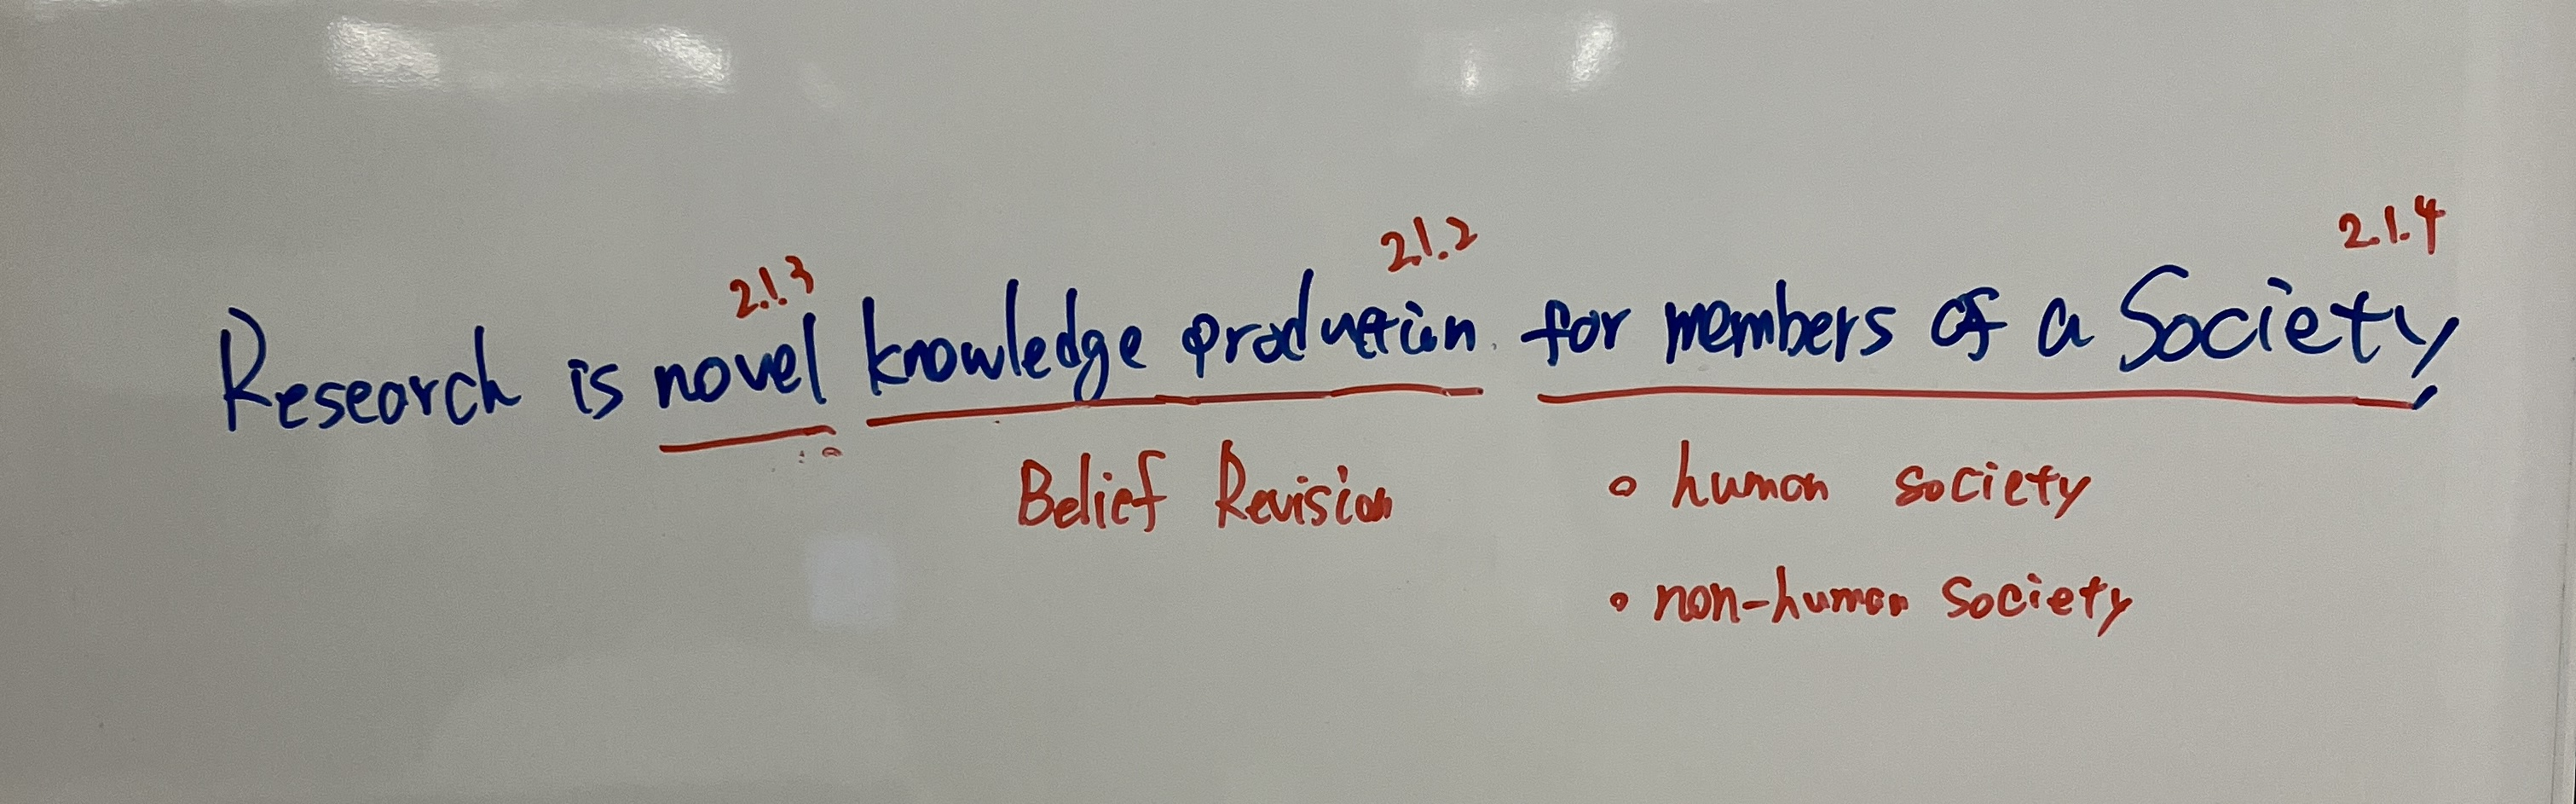
\includegraphics[width=\linewidth]{figs/definition.jpg}
    \caption{Definition of Research}
    \label{fig:definition}
\end{figure}

% \subsubsection{Some Notes on Research and Science}

The reason why I deliberately use the word ``research'' instead of ``science'' is because I want to include fields like engineering, humanities and arts, which are not typically referred to as science, within the scope of automation in the long run. Science refers to a methodology for generating knowledge, and I believe that new knowledge is not necessarily produced only by scientific methods. I believe that so-called humanities and arts also share some commonality of producing new knowledge. Therefore, the definition of generating new knowledge can be said to encompass these fields as well.

Of course I admit that science is the most rigorous and reliable framework for knowledge production. Because of its power and popularity, most of the existing analysis on research is about science. My discussion would also be centered around the discussion of science, though I try to present the view not limited to science. 

Please note that this definition is provisional. By viewing research as the production of knowledge, I can indeed characterize the wide range of current research activities of humans comprehensively, which is why I adopted this definition. However, as I will see later, difficulties also arise when defining it this way. Perhaps in some cases it might be better to focus on natural science and define research more narrowly as something like ``finding patterns in nature''. Defining what constitutes research is a challenging issue, and I believe that researchers should spend time discussing this definition, as I aim to create AI that can conduct research. The purpose of creating AI capable of research and how I should perceive the act of research should be discussed further in the future.

\subsection{Knowledge Production as Belief Revision}
I have defined research as the generation of new knowledge. Then, what exactly is knowledge, and what does it mean to produce knowledge? I will explore this question in this section. 

Defining knowledge and knowledge production rigorously is a philosophical debate that has not yet been settled \cite{sep-epistemology}, and I won't delve into it deeply here. Instead, I would like to provide some primitive ideas that can serve as a starting point for further discussions on how to realize an artificial researcher.

\subsubsection{Knowledge as Belief}
The question of what is the thing called knowledge has been a subject of debate for a long time in the field of \textit{epistemology}, which is one of the branches of philosophy. In epistemology, knowledge has been traditionally considered to be \textit{justified true belief (JTB)} \cite{sep-epistemology}. The term ``true'' is difficult to define rigorously, but for the purpose of discussion, let's think of it as something being fact. ``Belief'' can be provisionally understood as someone's thought or conviction about something. And ``justified'' means that it is deemed reasonable to hold such a belief. The meaning, necessity, and sufficiency of justification has been discussed in epistemology as a central point of contention. Since I am not well-versed in epistemology, I will refrain from delving into detailed discussions on that topic as it would go beyond the scope of this paper.

Of course, there is much debate about whether JTB truly is knowledge, and many philosopher agree that JTB is not the sufficient condition of knowledge. While these characteristics are not be sufficient conditions, there seems to be generally some agreement that they may be necessary. As epistemological discussions revolve around these notions, they seem to provide a reasonable starting point just for the purpose of my discussion. Therefore, for the sake of further argumentation, let's tentatively understand the generation of knowledge as the process of justifying, validating, or confirming beliefs about a truth.

\subsubsection{Knowledge Production as Belief Revision}
I believe that viewing research as an update of beliefs is somewhat reasonable. For example, let's consider a scenario where a hypothesis is proposed for a certain phenomenon, and then it is subjected to a test. This is a common practice in research. Now, suppose that through this testing, the hypothesis has been validated. This means that as a result of the test, my belief that the hypothesis is true has been strengthened. It could be said that this is an update of beliefs. Therefore, the view that research involves the update of belief seems to be reasonably valid.

% In the nature of research, which aims to generate new knowledge, it is necessary to engage in inference and justification regarding the unknown. Even if a hypothesis is not explicitly stated, some form of implicit hypothesis generation and testing should occurs in research. Therefore, the view that research involves the update of belief seems to be reasonably valid.

Let us explain a bit more about the reason why I deliberately say ``my belief that the hypothesis is true has been strengthened'' instead of just claiming that ``hypothesis turned out to be true.'' This is partly because, in almost all fields that rely on empirical methods, except for deductive disciplines like mathematics and logic, it is often impossible for verification to definitively determine if a hypothesis is true or false. Most research evaluates the validity of a hypothesis based on observations, relying on inductive reasoning \cite{sep-scientific-method}. However, inductive reasoning is unable to determine the truth or falsehood of propositions as deduction does without assuming some assumptions \cite{sep-induction-problem}. Even though we cannot judge if the hypothesis is true or false, we can still argue that the evidence obtained through verification makes us feel more confident that the hypothesis is true or false. This belief update holds for both empirical and deductive research. Thus, I do not say 3that a hypothesis became truth but instead say that my belief is updated.

I don't totally believe that because inductive reasoning doesn't rigorously determine truth or falsehood in the same way deduction does, it renders the reliance on inductive reasoning meaningless. This is because the assumptions that are said to make the inductive reasoning valid would sound natural to most humans and leave little room for doubt. As an example, it is said that we need to assume that ``under the same conditions, the same phenomenon will continue to hold'' (principle of uniformity of nature) \cite{sep-induction-problem}, which is an intuitive and natural assumption without which we could hardly even go about our daily lives.\footnote{
I understand that justifying the validity of inductive reasoning based on our experiences would be circular reasoning. The problem of what assumptions make us inductive reasoning consider rational is a challenging unanswered philosophical issue, which is beyond the scope of this paper. Thus, I will refrain from delving into the details here and leave it for future discussion.
} 

For the same reasons, I do not believe that the concept of belief being subjective makes it unsuitable for characterizing research. What I want to emphasize here is that research can be seen as linking or replacing the weak belief in the plausibility of newly conceived hypotheses with such extremely strong beliefs. For example, believing in the effectiveness of statistical methods is strongly related to believing in the effectiveness of inductive reasoning. Therefore, if the validity of a hypothesis is confirmed using statistical methods, we would believe it as highly reliable. Hence, considering research as the updating of beliefs can be reasonably felt, and I don't intend to argue that research is meaningless just because it is the belief revision.\footnote{
I naively assume that beliefs rooted directly in perception are more robust, and the notion that anchoring a belief on those foundations enhances its reliability. However, the question of how to justify beliefs is a complex problem with extensive discussions \cite{sep-epistemology} (my position seems to align somewhat with what is called \textit{empirical foundationalism}).Due to my limited philosophical knowledge and the ability to delve deeper into philosophical discussions, this paper will not further pursue these arguments.
}


% Therefore, while I don't know what exactly constitutes the basis of inductive reasoning, it would seem to be a deeply rooted and unwavering belief that is grounded in my perception and experiences. 

% \textcolor{red}{TODO: Add excuse for empirical foundationalism}
% The idea that there is ``strength'' in beliefs may be related to a position called \textit{foundationalism} in epistemology, which claims that ``\textit{my justified beliefs are structured like a building: they are divided into a foundation and a superstructure, the latter resting upon the former. Beliefs belonging to the foundation are basic. Beliefs belonging to the superstructure are nonbasic and receive justification from the justified beliefs in the foundation.}'' \cite{sep-epistemology}. In particular, I believe that the more fundamental beliefs to which these beliefs belong are rooted in human perceptual experience and empirical knowledge. This position is commonly referred to as \textit{empirical foundationalism} \cite{sep-epistemology}.

\subsection{Novelty of Knowledge}
No matter how firmly a belief is confirmed, if it is already known, it cannot be called research. Therefore, we have defined research as the process of producing ``new'' knowledge. In this section, I will briefly discuss what would it mean for knowledge to be unknown or novel.

As mentioned later, research can be described as the act of posing questions, proposing hypotheses in response to them, and then verifying those hypotheses to update beliefs on whether the hypotheses are correct. Therefore, it can be said that when knowledge born from research of a question is considered new, it refers to a situation where there has been no hypothesis that everyone believes to be sufficiently plausible for the question\footnote{
While presenting a question that no one has posed ensures that the knowledge is new. Even in such cases, no one also yet knows which hypothesis is correct for that question. This is why I have mentioned only about the unkownness of hypotheses
}. For example, we do not know how to create a general-purpose artificial intelligence, which can be said to mean that we do not have an answer (a hypothesis with high confidence) to the question, ``How do you create a general-purpose artificial intelligence?''.

% I said in the paragraph above that ``research is the process of transforming the unknown into the known.'' However research can also be seen as the updating of beliefs, as I have explained. Therefore, the binary depiction of an object suddenly transitioning from the states of unknown to known does not seem appropriate. Rather, it seems more reasonable to consider that beliefs continuously change and I just call some group of belief states unknown and others known, for convenience.

% I don't know precisely what it means to be unknown. This is a difficult problem, but let's consider it naively. 
% I consider a knowledge to be unknown when for a question a subject lacks any hypothesis which he/she has a JTB that the hypothesis is true. For example, I do not have the answer to the question of ``How to realize an artif icial general intelligence.'' So the knowledge of ``the way to realize an artificial general ingelligence'' is unknown. \textcolor{red}{TODO: Add explanation}

In research, a single verification does not always immediately turn a hypothesis into true or false. Rather, hypotheses that withstand repeated verifications through various experiments by different researchers gradually come to be regarded as more plausible. Therefore, it seems to me appropriate to say that research transforms a hypothesis with low confidence into one with higher confidence, rather than turning the unknown suddenly into the known. In that sense, it seems somewhat justified to describe new knowledge as something for which there wasn't a highly confident hypothesis before.

% The expression ``unknown'' could be more appropriately expressed as ``high degree of unknownness''. Because knowledge production is a continuous concept of belief updating, therefore, unknownness is also a continuous concept. In reality, there are multiple hypotheses with varying degrees of certainty concerning a particular question. The state of knowledge being unknown can be expressed as not having any hypothesis among these hypotheses with a particularly strong level of justified certainty.

% First, research begins with a particular question. The state of not knowing the answer to this question is what I consider the state of being unknown. In other words, it can be thought of as a state where I don't know what the candidate hypotheses, which are the potential answers, are like, or a state where I know the candidate hypotheses but don't know their plausibility. These are states where I have not been able to find hypotheses or sets of hypotheses that can be assigned a particularly high degree of confidence from the set of potential answers to a given question. Therefore, provisionally and casually, it might be said that the state of ``not having highly confident beliefs (or a set of beliefs) for a particular question'' is unknown, and the state of having highly confident justified beliefs is known.

% Of course, there are issues with this clarification. For example, it is unlikely that I can select a single highly confident hypothesis from the entire set of possible hypotheses. Also, rather than feeling equally confident about all possible hypotheses, it seems that I implicitly distinguish between hypotheses that seem relevant and those that do not. Furthermore, it is unclear to what extent I consider a state to be unknown based on the degree of confidence. However, these are highly challenging philosophical discussions, so I will refrain from delving further into them and, for now, would like to conclude with the vague and provisional definition above and move on to the next topic.

\subsection{Publicity of Knowledge}
\subsubsection{Knowledge as Human Knowledge}
The knowledge generated through research seems to be required to be knowledge for humanity. In reality, even if it is a strong belief, one person's belief is not recognized as knowledge unless other researchers gain a similar level of conviction from the research. Beliefs, knowledge, and understanding are indeed subjective concepts by nature, but it seems that we demand that they go beyond subjectivity and become comprehensible to others as well. 

Since knowledge production is belief update, generating knowledge for humanity requires updating the beliefs of all, or at least certain number of, people.\footnote{
Even if the knowledge is not immediately understandable, it should be potentially understandable to a considerable number of people. This means that the generated knowledge is not only for the society at the time of its production but also for the broader humanity, including future human societies. For instance, it might be challenging for children to determine whether the research outcomes in physics qualify as knowledge. However, by studying physics extensively, they may eventually comprehend cutting-edge research in the future. 
}\footnote{
Because it's impossible for different individuals to have exactly the same belief, as long as a justification can update the beliefs of different individuals in a similar direction in some way, I think it sufficient to be regarded as updating shared beliefs.
} 
It seems that researchers achieve this by verifying hypotheses in a manner that any human could find convincing. For instance, while most empirical scientific research verifies hypotheses through hypothesis testing, it seems that this is because results deemed plausible through statistics or inductive reasoning are thought to be plausible by virtually any human.

% Therefore, I believe research is the act of not only changing an individual's belief but also changing multiple individuals' beliefs. 

% Although I don't think it is possible for multiple people to hold exactly the same belief or for their beliefs to change in exactly the same direction, I at least need to use a way to change a collection of human beliefs in a similar direction.

In other words, this can be said to underscore the plausibility of the belief that ``a hypothesis is true'' with the extremely robust belief that ``inductive reasoning is valid.'' These robust beliefs seem to have been shaped through the process of evolution for the long time, being rooted in humans biologically. It seems that because science appeals to such fundamental beliefs inherent in humans as biological entities, its verification manages to convince many people.
% are rooted in our biological structures and perceptions acquired through the processes of evolution and development, as briefly introduced in the preceding section. For instance, beliefs such as the validity of logical reasoning, the uniformity of nature, and the tendency to find something more credible with an increase in observations fall into this category of beliefs. 

% And I believe that I achieve this by reducing hypotheses to strong convictions that everyone, regardless of individual differences, possesses as human beings. For example, assumptions underlying inductive reasoning, as I described earlier, will fall into this category. Another strong conviction humans believe in is that the more I observe an increasing number of results derived from a certain hypothesis, the more reliable and certain that hypothesis feels. Research need to be objective because it's required to generate knowledge for humanity, and I believe it is because I strive to reduce hypotheses to such strong convictions that it is called objective. 

\subsubsection{Knowledge as Non-Human Agents' Knowledge}
I said that research is to generate knowledge for humanity. However, this is merely because humans have been the ones conducting research thus far. I believe that in principle there could be knowledge for beings other than humans and hence research for them as well. A group of agents, each capable of holding certain belief states and having some level of similarity, seem to be able to hold a shared belief. If these agents have a way to ground their belief that a hypothesis is true to their shared belief, then this can be regarded as research within that society. Therefore, I define research as producing new knowledge for a society, which is not necessarily human society but also includes non-human agents'.

\begin{figure}[htb]
    \centering
    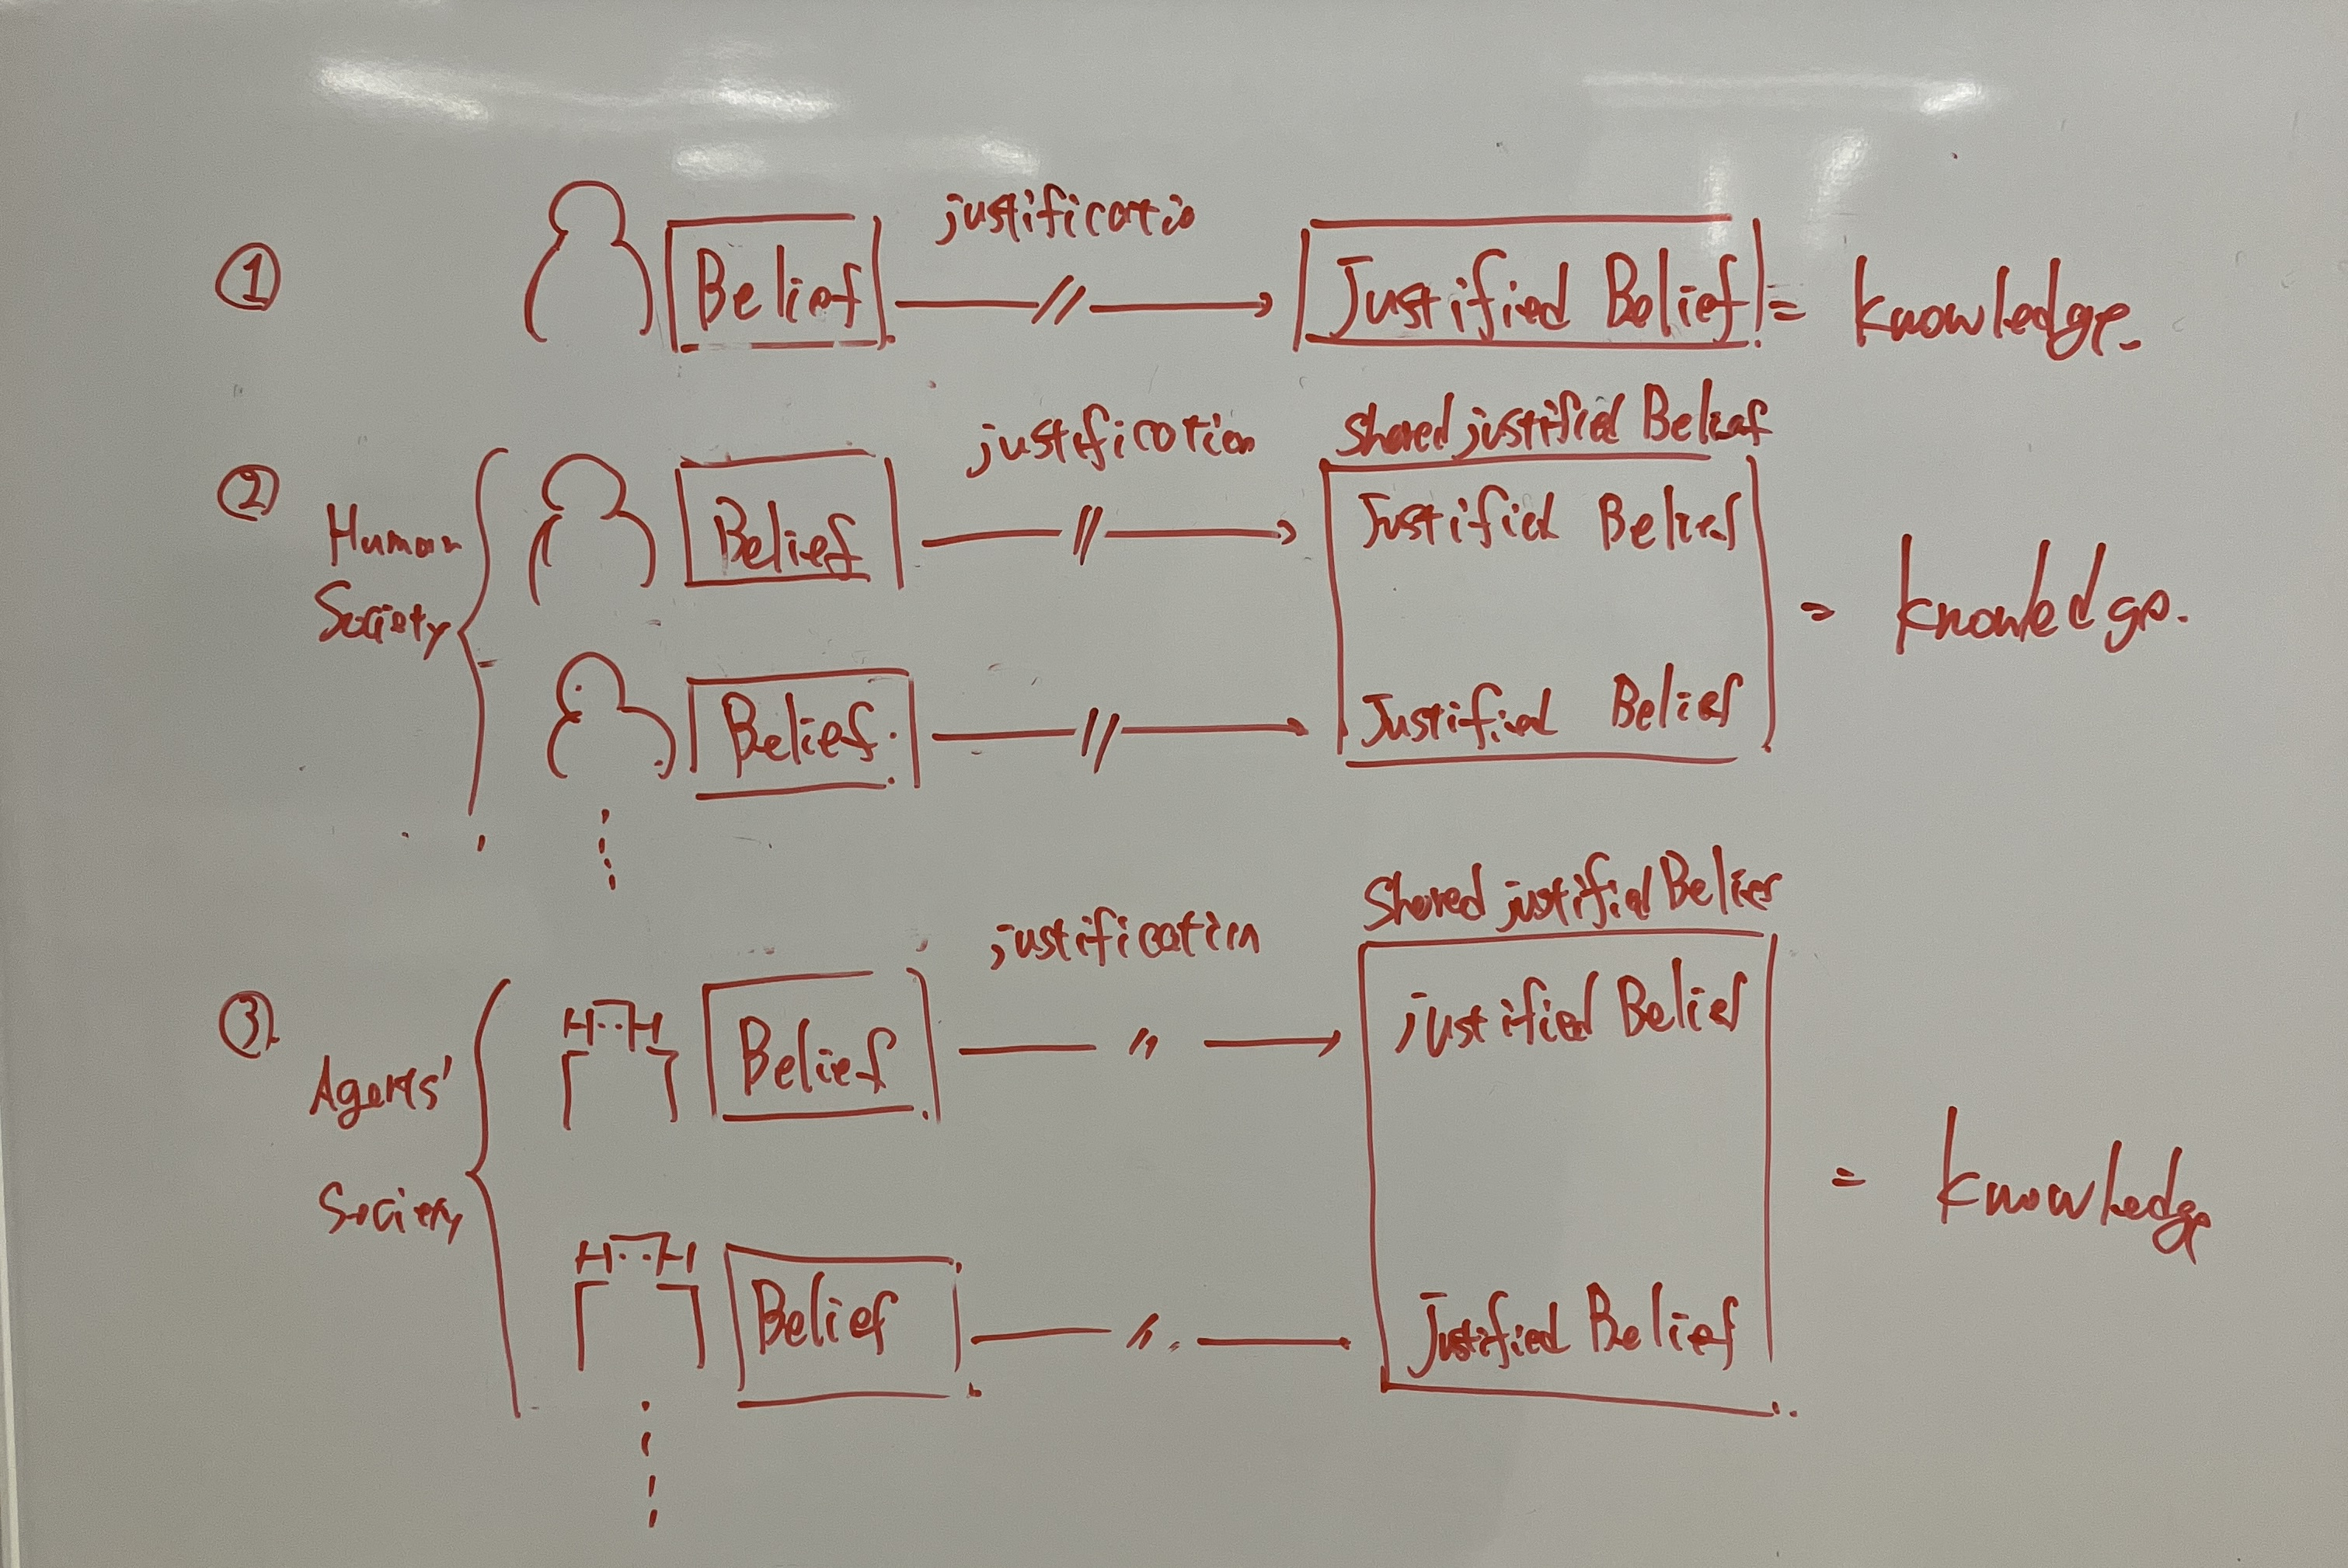
\includegraphics[width=\linewidth]{figs/shared_belief_revision.jpg}
    \caption{Belief Revision}
    \label{fig:shared_belief_revision}
\end{figure}

There are two implications here. Firstly, fully autonomous artificial researcher would produce nonsense for humans. This is because, even if a group of agents grounds their justifications in solid shared beliefs, it would be mere gibberish for humans if it is not shared among humans.\footnote{
This is akin to Khun's incommensurability \cite{kuhn1962}. 
} A straightforward way to solve this problem is to align the verification methods with those of humans. If we machines to execute even the verification methods entirely autonomously, it is essential to ensure some commonality with the methods humans use, which seems extremely challenging. This issue is essentially related to the problem of aligning human values with AI, and it is an extremely difficult problem.

% This implication means that if I want non-human agents to produce meaningful knowledge for humans, I need to ground it not in their shared beliefs but in human shared beliefs, or somehow ensure a commonality between these two sets of shared beliefs. If I aim for the former, the non-human agents may no longer be considered as conducting research in the same sense as humans. Additionally, regardless of whether I pursue the former or the latter, the problem remains of how to impart human shared beliefs to these agents, which is a fundamentally challenging issue. This issue is essentially related to the problem of aligning human values with AI, and it is an extremely difficult problem. I shall discuss this point separately.

% Certainly, even if I could share belief systems, if knowledge or the processes involved in acquiring knowledge were expressed using entirely incomprehensible systems for humans, it would still be meaningless to us. Therefore, if I seek to generate knowledge that is practically meaningful to humans, it seems essential for both humans and these systems to utilize, at the very least, a common representation format for knowledge, such as human language.

The second implication is that the artificial researcher would not even produce knowledge meaningful for understanding nature. This is because while human beliefs have been shaped to be consistent with nature through interactions with it, the beliefs of machines are not necessarily so. Through the process of evolution, humans have spent vast amounts of time interacting with and modifying their bodies to survive in nature. Our beliefs are formed in such contexts, and the beliefs we currently possess are likely advantageous for living in nature. Therefore, I believe that our strong belief serves as a reliable foundation for understanding nature. Machines do not possess bodies embedded with such interactions with nature. Therefore, just because they have strong convictions does not guarantee that these will serve as a reliable foundation for explaining nature. This seems to be a more serious issue than the first implication.

% In other words, the essential information for explaining and predicting nature is already internalized in my strong beliefs. It is precisely because I can trace these beliefs back to such interactions that I have been able to produce knowledge that deepens my understanding of nature. Now, suppose an agent has had no interactions with nature whatsoever until now. In that case, it seems highly unlikely that such an agent could acquire beliefs that are in harmony with nature. This goes beyond merely stating the importance of embodiment for AI. It suggests that an immense amount of interaction and learning, enough to form highly strong beliefs and internalize nature, is required and that learning these elements are inevitable for comprehending the natural world. 

\begin{figure}[htb]
    \centering
    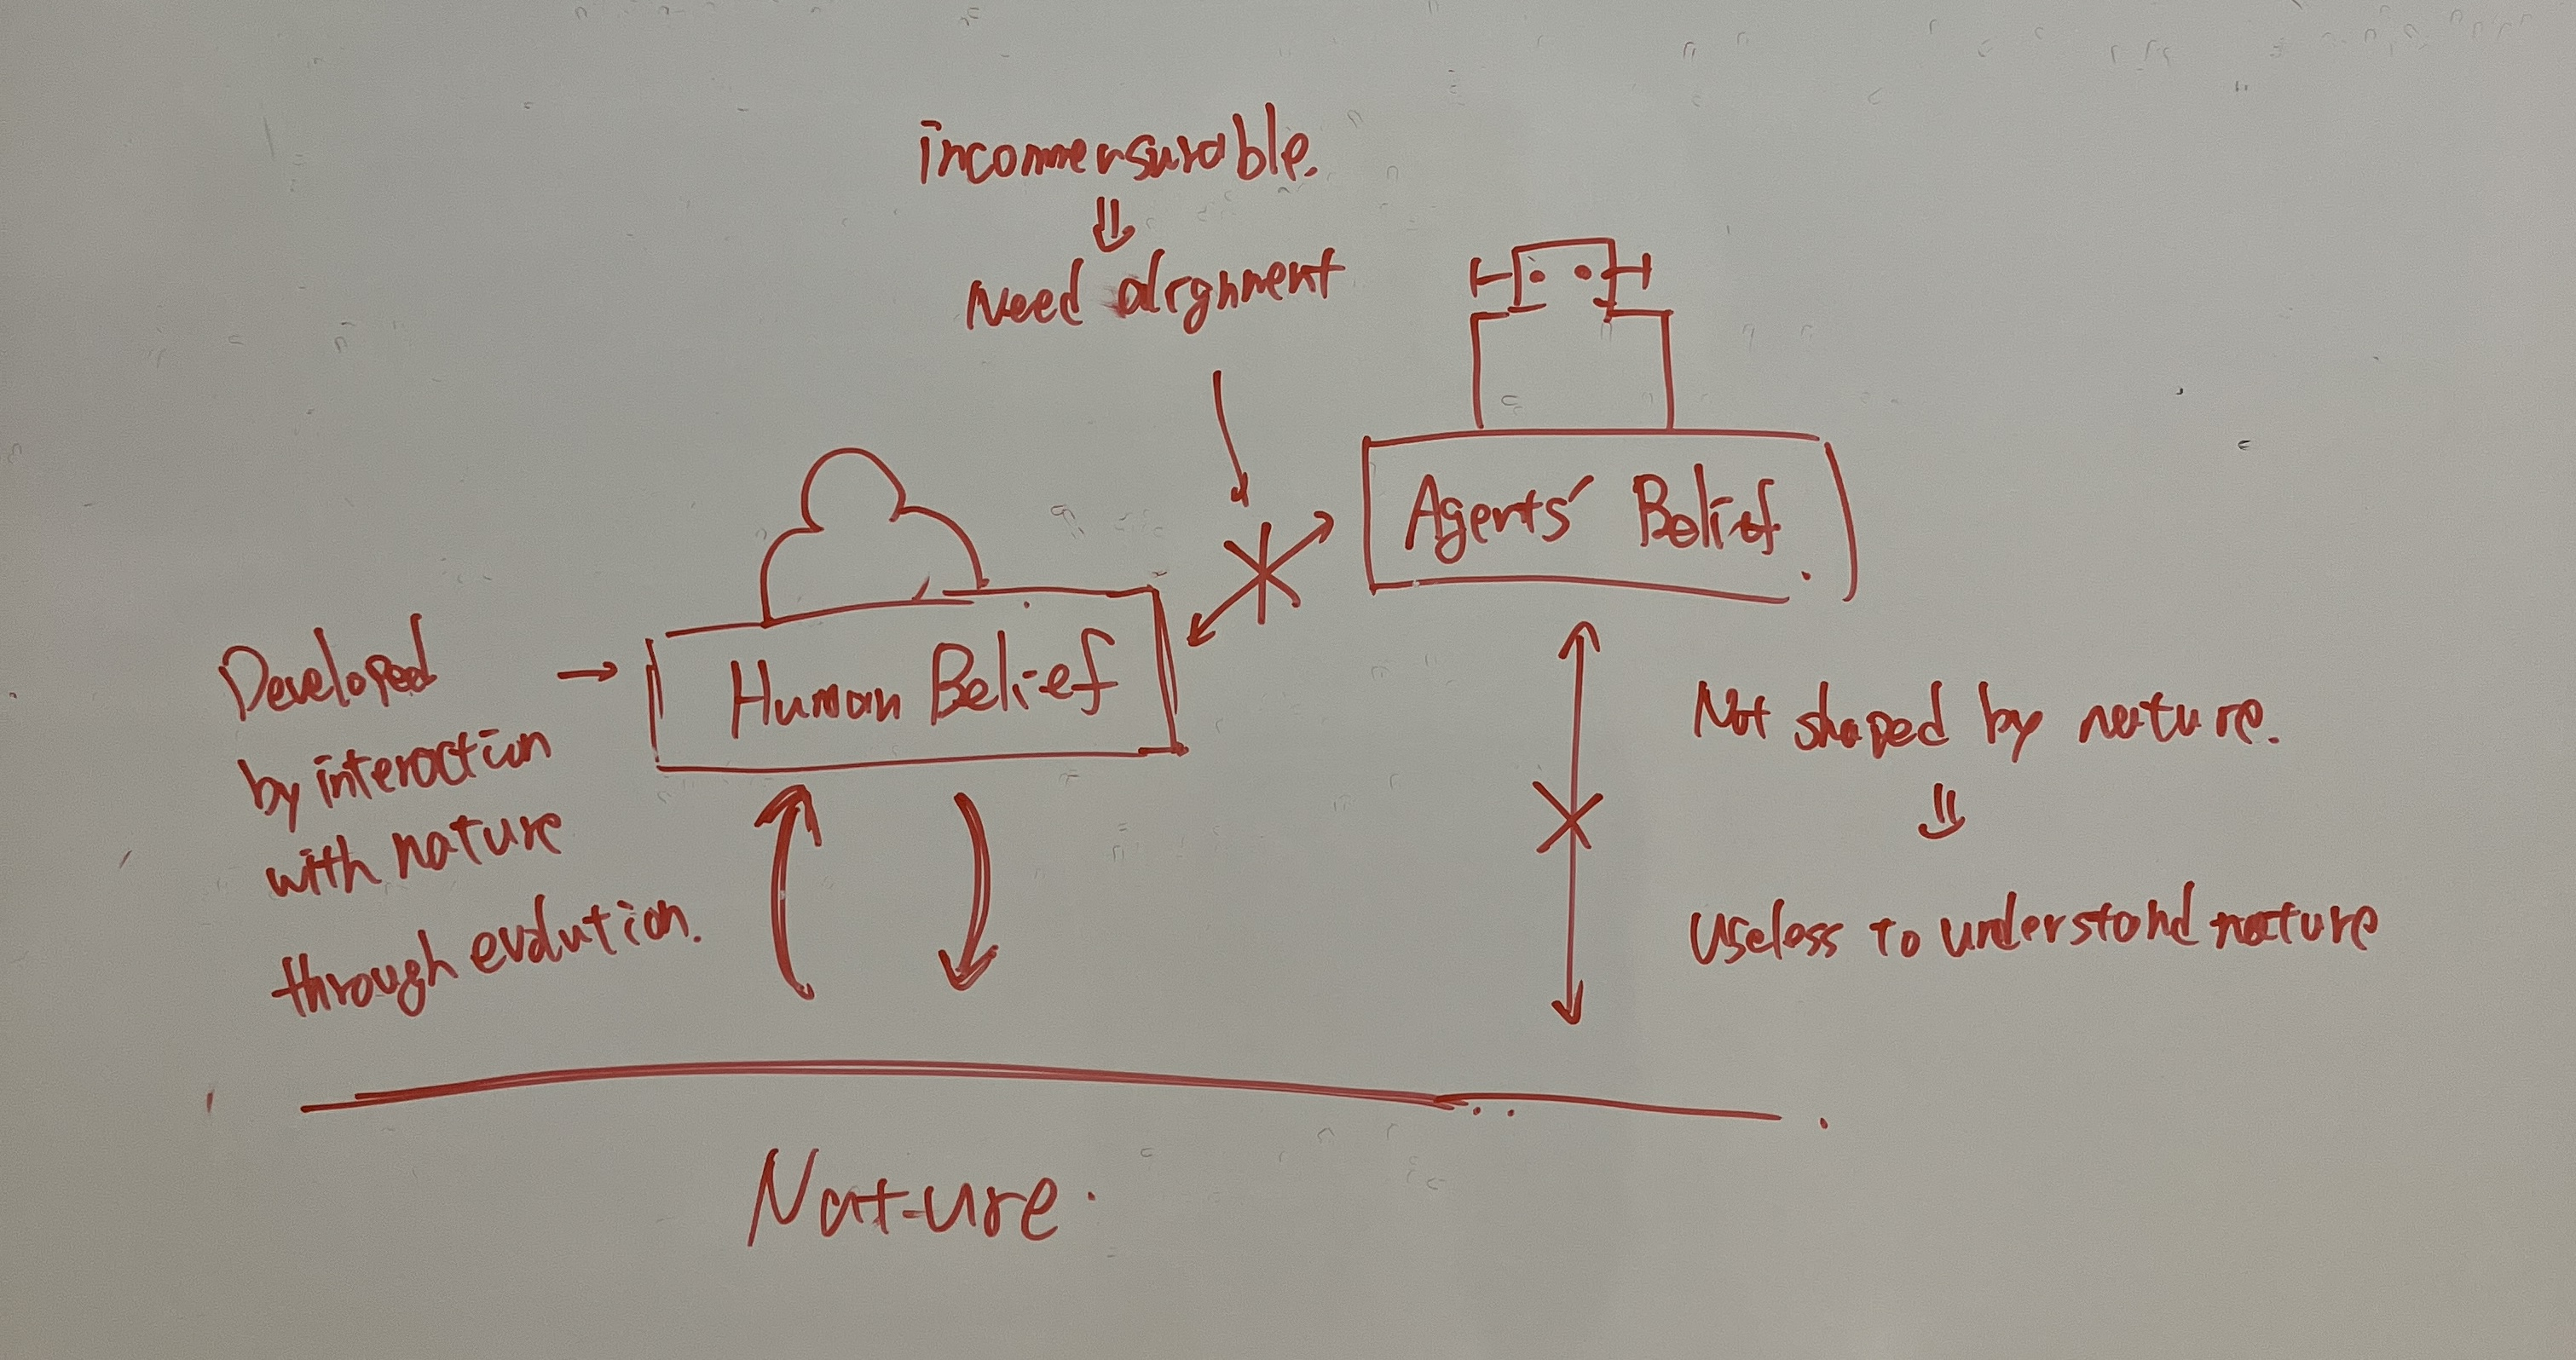
\includegraphics[width=\linewidth]{figs/incommensurability.jpg}
    \caption{Incommensurability}
    \label{fig:incommensurability}
\end{figure}

% First, knowledge is based on beliefs, so if a non-human agent holds beliefs, it would be reasonable to consider that they possess knowledge, even if they may not resemble human knowledge on the surface. The nature of beliefs is a complex matter to define concretely. However, even in current machine learning, models have confidence levels and prediction errors, which I believe are not completely unrelated to what I consider beliefs. Furthermore, even if the knowledge is not understandable to humans, if it is understood among a group of agents, meaning it is reduced to a shared belief, then it can be called ``knowledge for that group of agents.'' If a group of agents has means to update a belief to such a strong shared belief, then I consider it as research. From these reasons, I believe that research is conceivable for entities other than humans. And it feels like this is a highly significant conclusion in terms of contemplating the development of intelligent systems capable of conducting research.

% \textcolor{red}{TODO: Add relations with relativisim, maybe added to alignment section?}
% This position may have some similarities with a famous stance in philosophy of science that argues everything is, at its core, subjective, relative or a matter of belief \cite{chalmers2013thing,kuhn1962,howson2006scientific}. However, what I want to emphasize here is that I think the characteristic of research lies in tying beliefs about an object to stronger beliefs. And I believe that it is this strength of conviction, which seems self-evident to many people, that lends objectivity and persuasiveness to the claims of science.

% This is not definition but practically I think that one characteristics of research is its rigor of confirmation method. Firstly, you may wonder if anything unknown would suffice. I believe that research does not choose its subject and anything unknown is acceptable. Rather, what's important is the strictness of the methodology – whether the unknown truly became closer to the known, whether it was concluded into a stronger belief. Generally, the method employed by what I call research is designed with extreme precision, and as a result, it seems to withstand rigorous evaluations. This can be considered a major feature that distinguishes research from other various activities.

\subsection{Alternative Definitions}
I have adopted the definition that research is to produce new knowledge for a society. While the current definition of research was useful for a comprehensive discussion, adopting this definition led to counterintuitive conclusions and seemingly intractable problems. Therefore, there might be debate over whether we truly want an artificial intelligence capable of research in this sense. In this section, I would like to discuss the possibility of alternative definitions of research.

\subsubsection{Limited to Human Knowledge}
One of the biggest issues is that a fully autonomous artificial researcher is likely to produce knowledge that is meaningless to humans, or even more so, not connected to an understanding of nature. Thus, one alternative proposal is to limit what an artificial researcher produces strictly to knowledge that is relevant for humans. Notably, this problem arose entirely from allowing artificial intelligence to autonomously construct even the foundation for validation. Therefore, what this alternative definition demands is to ensure that the foundation for validation remains fundamentally human.

This is somewhat less restrictive than ``producing knowledge that humans can understand''. That's because it is conceivable that there is a procedure where humans might be convinced something is true if that is confirmed by the procedure even if they can't fully grasp the details of the mechanism of the procedure It seems that what most people desire is an artificial intelligence that produces knowledge understandable to humans, so for most people, this definition should be more than sufficient.

One downside of adopting this definition is that it might preclude the production of knowledge that, while certainly explaining nature, cannot be verified within the framework of human validation. If one believes that nature transcends human cognitive limitations, it seems reasonable to assume that such knowledge exists. While this may not be a concern for most people, it seems to be a significant constraint when considering ``how far nature can be understood beyond human limits.''

% This all arises due to the expansion of the definition of research to include non-humans. Consequently, it is possible to aim for a definition of research strictly limited to knowledge production for the human society, and to ensure that artificial researchers exclusively engage in research for the benefit of humans. This appears to be more of a decision-making issue about what kind of future I want to pursue, rather than determining which definition of research is correct. Alternatively, it might be worth reconsidering the definition of knowledge production as the mere updating of beliefs. Engaging in discussions about this problem seems to be of great importance for the future of human society.

\subsubsection{Knowledge Consistent with Nature}
There is also the perspective that if we truly understand nature even if it's beyond human comprehension, then that's not a problem. However, there were concerns that machines, not having interacted with nature like humans have, might produce knowledge based on their beliefs that does not lead to a true understanding of nature. Therefore, the second alternative is to impose the constraint that the belief system must always be consistent with nature. In this case, it would be necessary to first allow the machine to interact with nature and then have it form a belief system that aligns with nature. However, I don't know what that might look like or how it would be constructed.

If it turns out that the knowledge system might not always be comprehensible to humans, then we face the issue of being unable to confidently verify whether the artificial intelligence is truly producing meaningful knowledge in terms of understanding nature. Thus, if we adopt this definition, the alignment issue I mentioned earlier still remains. While there's the advantage that it might enable an understanding of nature beyond human limits, many people might not think it worth adopting this definition.
 
\subsubsection{Research as New Pattern Discovery}
One of the main reasons the definition I adopted lead to counterintuitive results may be because I regard research as the production of ``knowledge'', and knowledge as ``belief''. I interpret research as the updating of beliefs just because it is consistent with human research practices so far. Rather, an essential aspect of research seems to be discovering or creating something ``novel'', and whether or not that constitutes ``knowledge'' seems secondary.
% knowledge is JTB, which implicitly assumes that the generation of knowledge, i.e., research, aims at acquiring a truth. 

Given this, it might be worthwhile to simply define research as the ``discovery of new patterns (in nature)''. This definition seems to at least encompass our current research endeavors. It emphasizes the discovery of new things, is not dependent on the subject, and, (by specifying ``in nature'',) appears to align with the goal of understanding nature.

This might be too abstract, so it would be necessary to re-analyze what this definition truly means. I'd like to consider that discussion as future work.

\subsubsection{Research as Question Answering}
Defining research as merely a question-and-answer process might be one approach. However, a distinguishing feature of research is that the answer is unknown to anyone. Nobody knows the correctness of the answer, but it is indirectly provided by the subject of study, such as nature. While it's unclear to what extent this formulation can alleviate the issues with the definition we've adopted, it seems worth considering for furhter study.

\subsubsection{Pragmatist Epistemology}
Up to now, following the tradition of epistemology, we have assumed knowledge to be JTB. That is, we have been evaluating the justification of a belief based on how close it is to the truth. However, there is also a position that evaluates beliefs not by whether they approach truth but by whether they are useful for human or not. This position is known as \textit{pragmatist epistemology}. 

From this perspective, it could be possible to argue that the outputs of current machine learning models, for example, may be considered knowledge since it shows high predictive performance, leading humans to the desired behaviours. In this sense, this position is highly compatible with statistical machine learning \cite{otsuka2022thinking}.

As such, this pragmatism presents a different view of research from that of majority of researchers, and it could be seen as advocating a redefinition of the act of research. Many researchers may not accept this view. Nevertheless, in recent years, deep neural networks have made rapid advancements and have produced many ``useful'' outcomes in research, which has made the debate on whether to consider their outputs as knowledge much more relevant and realistic than ever before.

In this paper, I take the position that knowledge is JTB, and research is an endeavor to approach a truth. Therefore, I will not address this issue in the following sections that much. However, we must seriously consider the implications presented by deep neural networks and delve deeper into the discussion of how we should define research, what constitutes research, and what purpose research serves.

\subsection{Interim Summary}
In this section, I have discussed a provisional working definition of research. I started with the naive intuition that research is the endeavor to generate new knowledge for a society. I then explained that knowledge is belief, the production of knowledge involves updating beliefs, and the produced knowledge needs to be novel and supported by the common strong beliefs of a community. Lastly, I discussed based on these conclusions the possibility of research conducted by agents other than humans.

% Reflecting on what research entails is highly important as it provides clarity on what we should truly make. The discussion in this chapter suggests us that we need to discuss how to instill these abilities to artificial intelligence so that we realize an AI to conduct research.

The definition discussed here is merely a provisional one based on the naive intuition. By combining insights from philosophers, scientists, and all working researchers, we can engage in a deeper analysis of the definition of research, developing more fruitful and reliable guidelines for our goal.

% The reason I deliberately distinguished between mere knowledge and knowledge for humanity is because I believe that there could be knowledge for beings other than humans. As I have repeated, understanding is subjective, so if machines start conducting research in the future, it is natural to think that there will be unknowns for machines and beliefs for machines. Therefore, it's possible that I could live in a world where humans produce knowledge for humans, machines produce knowledge for machines, I could live in a world where knowledge is produced for all agents including machines and humans, or I could continue living in a world where knowledge is produced solely for humans. In this sense, I believe one of the problems that will be questioned in the future is whose objectivity and whose belief I am talking about. I will discuss this point in more detail later.

%%%%%%%%%%%%%%%%%%%%%%%%%%%%%%%%%%%%%

% When a hypothesis survives a test, it was said that my belief in the likelihood of the hypothesis strengthens. Empirical science implicitly assumes a principle that relies on inductive reasoning as the basis for these tests. For example, I believe that if the number of observations consistent with a certain claim increases, that claim is more likely to be valid (this is called the principle of confirmation). Additionally, I hold the belief that unless other factors change, what has held true so far will continue to hold true (this is called the principle of uniformity of nature). These principles of confirmation and uniformity are the foundations of inductive reasoning, and they are unavoidable in empirical science. However, both the principle of confirmation and the principle of uniformity are merely beliefs, and there is no guarantee anywhere that these are ``correct''. The reason these can serve as the foundation for testing is because these beliefs are far more solid than the belief in the likelihood of a hypothesis that someone has just recently presented. That is, empirical science could be described as an endeavor to update the likelihood of a hypothesis by tying the belief held about a certain hypothesis to a more solid belief. While mathematics and logic are rare examples, considering that all other research endeavors are fundamentally empirical, \textbf{it may be possible to rephrase the endeavor of research, that is, the production of knowledge, as largely an endeavor to update my belief in the correctness of a certain object.} In fact, it is widely accepted in philosophy that knowledge requires belief \cite{sep-epistemology}. More formally, it's believed that "\textit{the three conditions—truth, belief, and justification—are individually necessary}" for knowing a fact \cite{sep-epistemology}.


% \subsection{Disclaimer Regarding the Characteristics of Research}
% I have mentioned that research is an endeavor to transform the unknown into the known, but you may question what distinguishes it from other activities that appear to do the saus. This issue arises from the fact that I have not properly defined knowledge in this paper. In this paper, I won't discuss this in detail but will limit myself to a brief disclaimer.


% \subsection{The Previous Discussions Regarding the Definition of Research (Scientific Discovery).}

\subsection{Question Construction, Hypothesis Generation, and  Verification}

% \textcolor{red}{TODO: more focus on the implication for research automation}

% It is believed that research began with individual and concrete tasks. Among them, common actions were patterned and crystallized as a scientific method. I currently recognize this abstract set of behaviors as research. For example, hypothetico-deductive method and hypothesis testing are abstracted scientific method.

% Also, researchers use a research paper as a medium of knowledge transfer. Therefore, there are patterned activities related to a research paper. Examples of these include conducting surveys, gathering information from papers, and writing a thesis.

% Note that these are necessary tasks just because I use a paper as a medium of knowledge transfer, but they may not necessarily be indispensable for generating new knowledge. There are other such tasks as well. For example, peer review and fund raising are essential to current research practices in society, but they may not necessarily be indispensable for knowledge production.

% In this way, various tasks arise in conjunction with research. When considering the automation and optimization of research, it is desirable to consider streamlining all of these tasks. However, in this article, I focus on the process from determining a research topic to publishing a research paper. I will refer to this process simply as the \textit{research process} from here on.

% \subsection{Overview}

% As mentioned earlier, research is an attempt to turn the unknown into the known. Therefore, the research process can be seen as a function that takes the unknown as input and outputs the known. However, in reality, a single research paper may not be enough to turn the unknown into the known. Therefore, in practice, the research process is considered to be a procedure that takes the unknown as input, and outputs a text that describes the procedures and their results, as well as their interpretation, in order to turn the unknown into the known.

% First, let us structure the common research process. In particular, I will base the structuring of the research process on the method of empirical science, which many researches rely on as a foundation. However, I believe that this framework can be applied to other research activities, such as mathematics, as well. I will explain the reason for this later.

% The research process, especially that of empirical science, is carried out through the following steps: topic decision, hypothesis generation, verification design, verification, and analysis of experimental results. The outputs of these steps are then written into a paper, which undergoes peer review and is eventually published.

% Note that some commonly seen items, such as surveys, are not included here for a reason. First, as mentioned earlier, gathering information from papers is only a means of knowledge transfer through the use of a thesis. Second, information extraction from papers can be done at any stage of the research process. Thus, I believe that processing related to a paper, such as \textit{reading papers} and \textit{writing a paper}, needs to be considered separately from the aforementioned research process.

% \subsection{Overview}

% \textcolor{red}{TODO: reconsider the research process, structure of knowledge production system, and the scope of this paper}

The definition of research stated in this section is somewhat too abstract to serve as a concrete guideline for building something based on it. Moreover, it feels distant from the research practices employed by humans, making it challenging to immediately connect our standing point to with the goal. While the ultimate goal is to achieve a fully aunotomous system for conducting research, it is practical and useful to start by discussing how to realize individual sub-processes within the research process. Breaking down the research process into partial processes will make the functions that need to be achieved much clearer.

Therefore, I view research process as a \textit{knowledge production system} and attempt to structure the process by decomposing it into its constituting modules. During this division, each sub-process will be structured with the level of abstraction required for all types of research. This is because the focus of this paper is a general artificial researcher. 

% Hence, even if an element seems crucial in current research, if it is not necessarily essential to the definition of research seen so far, I will treat those elements separately from the constituents of the research process in this study. By separating these elements, I intend to clarify the indispensable components for realizing an artificial researcher. 

% \subsubsecti on{Outline of the Structure}
% In this section, I will discuss the three things tightly related to the knowledge production. I will first discuss the functionally essential elements for knowledge production system, which is the abstract structure of the research process that has been emphasized so far. These elements correspond to the modules in knowledge production system. This is a main topic of this chapter. 

% For convenience, I will refer to the entire structured research process as the \textit{knowledge production system} or just \textit{research process} throughout the rest of this paper.

% In the previous chapter, I discussed the definition of research. In this chapter, I will focus on the high-level abstract structuring of the research process while paying attention to its functional aspects. By emphasizing the functional aspects, I mean paying attention to the role that each step plays in knowledge production. By higher-level abstract structuring, I intend to focus on the processes that is as universal as possible across research fields, regardless of the specific domain. The purpose of this kind of structuring is to clarify what kind of modules should be created as intermediate steps of research when aiming for research automation. In the following, I will structurize the research process into a chronological sequence for the purpose of clarity. However, it is important to note that the focus lies not on the temporal order nor human convention, but rather on the functionality in relation to knowledge production and the inputs and outputs of each of these processes. Also, as previously mentioned, because humans are currently the primary knowledge generators, there are many constraints that come from human society. Thus I will do my best to distinguish and organize what is dependent on humans and what is not. Before delving into specific discussions, let us first explain the scope of this chapter. After that, I will discuss the outline to be addressed in this section, followed by the main discussions.


% \textcolor{red}{TODO: add the excuse that research is social activity}



% \begin{figure}[htb]
%     \centering
%     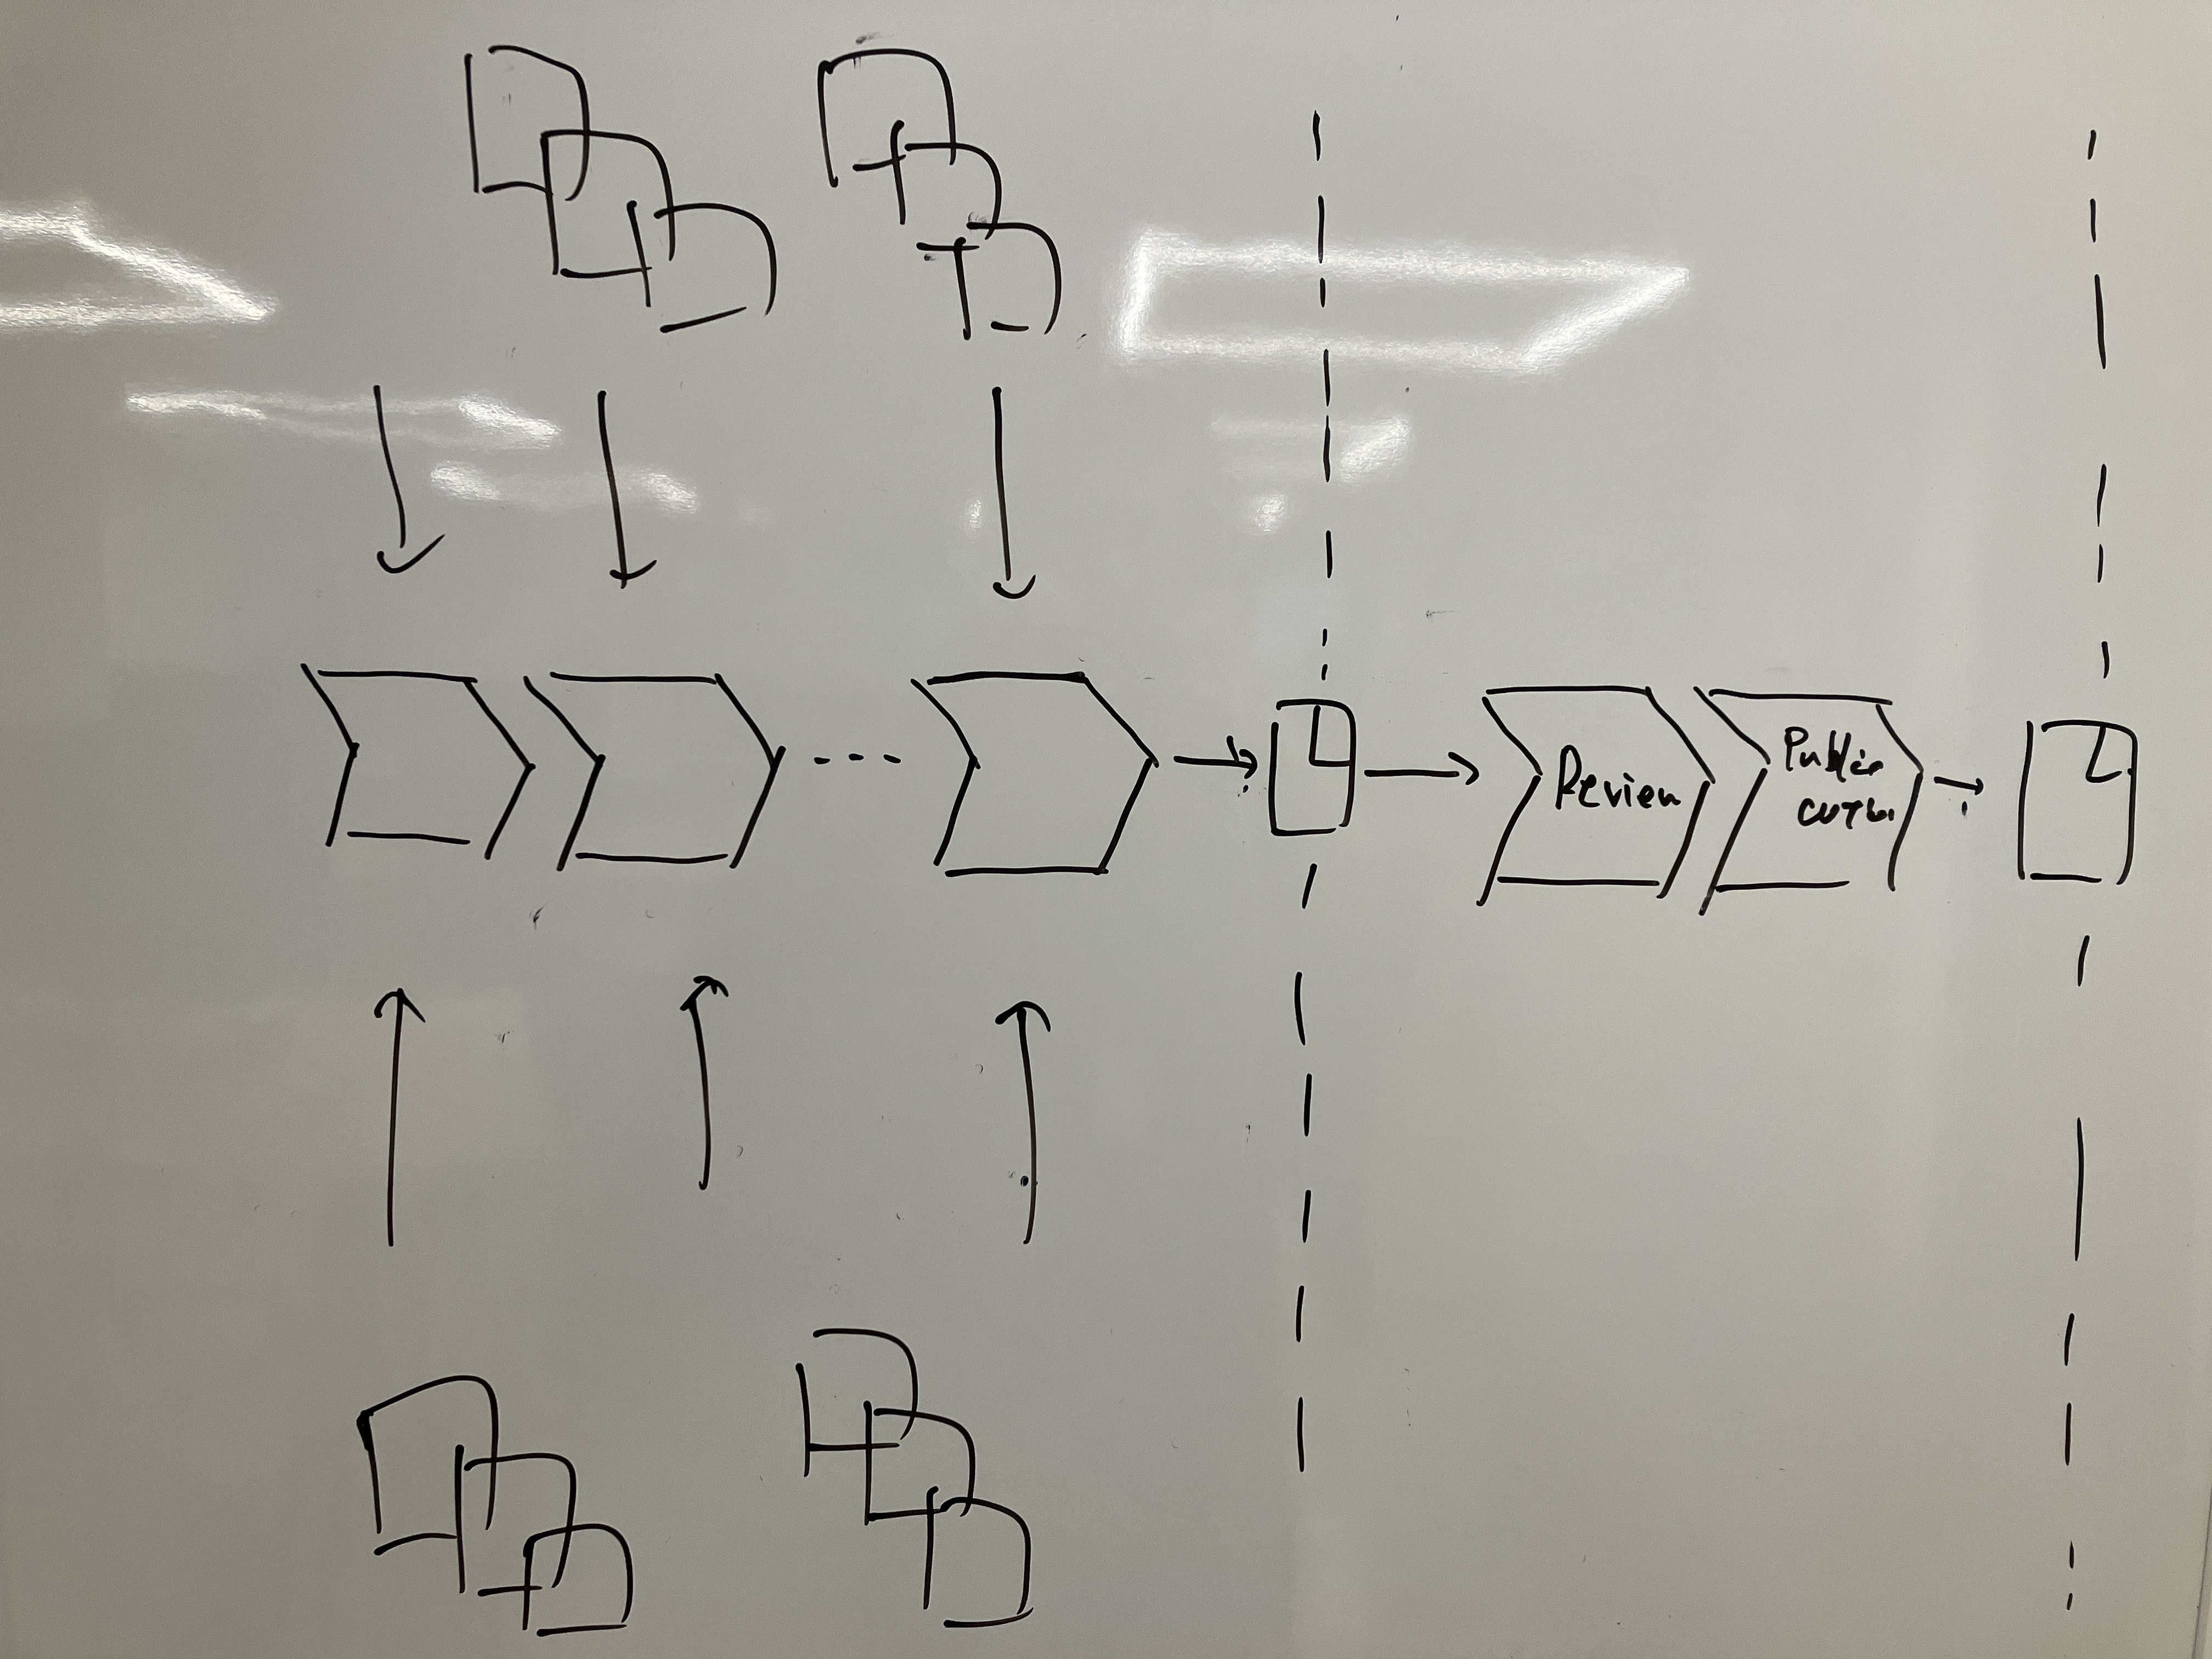
\includegraphics[width=\textwidth]{figs/researchprocess.jpg}
%     \caption{Caption}
%     \label{fig:research_process}
% \end{figure}


% Next, I will discuss a high level description of how human beings have been conducting research. I'll structurize the abstract pattern of the process (which I will call\textit{ research process}) from determining the unknown to it turning into known. 


% \subsubsection{Note}

% note, direction
% Though my structuring may seem to represent scientific methods, I believe this pattern cam apply to other research fields, such as mathematics and humanities as well. When describing the structure, I will make a conscious effort to clearly distinguish between essential elements for knowledge production and those that are not. As previously mentioned, because humans are currently the primary knowledge generators, there are many constraints that come from human society. When considering the possibility of machines conducting research in the future, it will be important to distinguish and organize what is dependent on humans and what is not.

% I believe that the conduct of human research activities can be roughly divided into three stages: knowledge production, knowledge evaluation, and knowledge sharing. 

% Although these may not necessarily be distinctly separable from each other, I adopt this classification because it is useful for advancing discussion. The process of knowledge production consists largely of the steps: problem determination, hypothesis generation, and hypothesis verification. And in this process, the ability to read and write documents and analyze data are required as necessary skills. Below, I will examine each of these in more detail. 


% This structuring is tentative and there may be a better way to structure the research process. However, I have created this structure for practical purposes in order to move the discussion forward. I hope the structure of this article be a starting point for conceiving a better structurization. I believe that structuring and deepening understanding of the elements that are essentially important for knowledge production is extremely crucial when aiming for the automation of research.

% Though I explained that research is belied revision, it would be convenient to see as a function that takes the unknown as input and outputs the known.  % TODO: rearrange

\subsubsection{Three Sub-Modules in Knowledge Production System}
In the following sections, I will explain three essential elements that I think are functionally necessary in knowledge production: \textit{question construction}, \textit{hypothesis generation}, and \textit{hypothesis verification}. These are the abstract structure of the research process that has been emphasized so far.

Constructing questions is equal to deciding the unknown to be investigated, which is necessary by definition for research, which is the art of bringing the unknown closer to the known. Since answering this question is the objective, hypothesis generation is necessary. The reason it's not just a simple question answering, but question construction and hypothesis generation, is because no one knows the answer of the question yet. The third process is hypothesis verification, which is a process that shows us how probable it is that a hypothesis is true. This is indispensable, as it is converting our beliefs that a hypothesis is true into knowledge.\footnote{
While the term ``verification'' is used here, it does not imply a definitive determination of the truth or falsehood of propositions. It is used in the sense of just strengthening beliefs as used in everyday language. Thus, ``confirmation'' may be a more accurate term, but verification is more widely recognized, so I will use that.
}

% When summarizing these intermediate steps, it goes as follows: First, upon receiving any input, I formulate a question. Taking this question as input, hypotheses are generated. Finally, these hypotheses are input and validated resulting in the creation of knowledge as a research outcome. These processes are considered a proper decomposition of the research process, as they request each other's outputs as inputs and seamlessly connect the entire research process from input to output without any gaps.
% \textcolor{red}{TODO: However, I can identify discovery with justification because both are belief updates. I'll add this point wherever in this paper.} Fig. \ref{fig:knowledge_production_system}.

% \textcolor{red}{TODO: Add fig like this. add this sentence to the explanation of the fig "we approach the unknown to the known by asking questions, providing tentative answers to them, and then verifying the validity of those answers. " }.
% Fig. \ref{fig:research_process}.

\subsubsection{Human Research Practice and Knowledge Production System}
In actual research, while addressing the initial question posed, another question may arise and the focus may shift to that new question. Also, before reaching the final hypothesis that gets reported, several different hypotheses are tested repeatedly. Like this, the actual practice of research is complex.\footnote{
For example, the concept of \textit{night science} as proposed by Yanai and Lercher symbolizes the such complex reality of research practice \cite{yanai2019night}.
} When compared to this trial-and-error process, the framework I have proposed may seem overly simplified at first glance. However, I believe that the framework I proposed encompasses these human practices as well.

The framework I presented claims that in the process of generating knowledge, there is always a construction of questions about the process, the generation of hypotheses, and the verification of these hypotheses. I have not specified how these are done. Therefore, a question might have arisen while working on a different question, or it might have been directly derived to achieve a specific goal. Similarly, a hypothesis might have been developed after multiple comparisons with real data, or it could be something that came to mind while walking. What I'm arguing is that, regardless of the diverse methods employed, when an activity is termed research, there should always be a stage where questions related to the knowledge produced, the generation of hypotheses, and the verification of these hypotheses are addressed. This may indeed look like a linear process when abstracted, but given that it allows for trial-and-errors as its internal implementation, I believe it encapsulates the complex practices of human research.

Furthermore, setting aside whether a strict methodology like that of research is required, I believe that all endeavors to transform the unknown into the known, to some extent, inevitably involve the construction of questions, the generation of hypotheses, and the verification of these hypotheses. In other words, I think this framework might be an embodiment of the very act of turning the unknown into the known. In this sense, this framework might be better understood as a fundamental unit in research.

\section{Question Construction}

The first module of research process should be question construction. This is because in order to produce new knowledge, one must first be aware of what they don't know and strive to generate that unknown knowledge. Questioning is an act of trying to fill a gap in the  information that the questioner possesses, and in that sense, the act of trying to produce missing knowledge for humanity is the very act of posing and answering a question.

% This is because research is an act of generating new knowledge, and questioning is the act of seeking missing information. 

% To initiate the process of generating new knowledge, one must first know what could potentially be new knowledge. In other words, we must know what I don't know. This is an essential function for research to be the production of new knowledge. And it is the task of question construction to fulfill this function. Therefore, question construction is an indispensable module in the knowledge production system.

The process of questioning involves two steps: 1. Recognizing missing information, and 2. Attempting to fill that gap. For example, the process of asking why the sky is blue starts as follows: when prompted by, for example the vision of sky to your eyes, you suddenly (with complex perceptual and cognitive processes) realize that you don't know why the sky is blue, and then, if you would like to know the answer, utter the question, ``Why is the sky blue?''\footnote{
Here, I explained the process of questioning as first determining something as unknown and then deciding if you construct question about the unknown. However, the order doesn't matter. For instance, there may be knowledge that you want to know first, and then you confirm that it is indeed unknown. What matter is that, to create a module for question construction, it would be necessary to consider how to achieve these abilities: recognizing missing information and deciding if you will do questioning. 
}

\subsection{What is Questioning?}
\subsubsection{Recognizing Unknown}
When prompted with a request for a specific type of knowledge and upon referencing your own knowledge base, if you judge that you do not possess that knowledge in your knowledge base, you recognize it as unknown to you. In the example of the blue sky, the knowledge of ``reason'' or the ``cause'' of the blueness of the sky is requested. Such demands for knowledge would likely be triggered by various factors (for example, attention may be drawn to the causal relationship between the sky and its blueness because one tried to explain why the sky is blue but couldn't). When you think about the request and cannot find the answer, you would recognize that you do not possess the knowledge. 

% Here, two things are happening. First, you refer your own knowledge, and second, assessing whether there is expected knowledge in your knowledge base. This means that recognizing the unknown can be understood as a combination of these two processes. I would like to delve into this in more detail in the following section.

% \subsubsection{How Human Judge Unknownness}
For an individual, the knowledge base is the memory within the brain. If certain knowledge is not in the memory, or cannot be constructed from other knowledge that is in memory, we would recognize that we don't know that knowledge. 

% In the case of an individual, the process of recognizing such knowledge as unknown seems to involve retracing whether they have the knowledge in your memory. When no relevant memories come to mind, the person may infer that they do not possess the knowledge. Even if the memory does not exist, they might try to use existing knowledge to answer the question. When they cannot construct a valid answer they are confident about, you consider it a recognition of not knowing. As mentioned earlier, to recognize a piece of knowledge as unknown means not having a justified belief that a proposition is true for a particular subject. Thus, the criterion for judging ``being unable to construct a confident answer'' can be seen as not having a justified belief.

% any ``memories'' of knowing, using, or hearing about that knowledge.

% While I have discussed recognizing unknowns for individuals, in research, what is essential is recognizing unknowns for society as a whole. If there is a way for an entity to identify societal unknowns without going through the process of identifying unknowns for individuals, that would be ideal. Therefore, I will discuss how to recognize societal unknowns.

In research, what interests us is not whether something is unknown to an individual, but whether it is unknown to humanity. In the case of research, the knowledge base consists of the collective media that records human knowledge, such as all the research papers, books, and articles on the web. Specifically, the most widely used method for determining novelty for humanity is through literature surveys of academic papers. If we examine as many academic papers as possible and find no prior research that has presented a properly validated hypothesis for the same question, we recognize that knowledge as unknown.\footnote{
n other words, in order to determine whether a certain piece of knowledge is unknown, one must also be able to judge whether a certain validation is valid.
} Even in a world where machines conduct research, this method of determining unknowns will likely persist. Therefore, an AI capable of research needs to be able to identify relevant knowledge and determine whether it has been appropriately validated.

The point of contention here is whether we accept something as unknown if an AI, based on its own memory, determines it as such. In human terms, something unknown to a single individual is not necessarily deemed unknown to humanity. Similarly, one might argue that just because AI, based solely on its memory, deems something as unknown doesn't mean it truly is. On the other hand, given that AI can potentially store vastly more knowledge than humans, there's a stance that if something is determined as unknown from such a vast memory, then it may well be accepted as genuinely unknown. This seems to be a topic that should be further debated in the future.

% Knowledge for humanity is primarily disseminated through research outcomes. Therefore, when examining all the research outcomes that have been generated thus far and finding that none of them provide an answer to a specific question, it seems reasonable to conclude that the question possesses sufficient uncertainty to warrant further investigation as a research endeavor. In particular, humanity has developed the culture to preserve the research outcomes in the form of papers. Therefore, it seems feasible to assess the unknown nature of an inquiry by examining all academic papers. There are various methods to determine whether the desired knowledge already exists. Typically, it is considered that candidates can be narrowed down in two steps. First, since research papers are composed of questions and their corresponding answers, one can search for papers that have similar questions and answers to the desired knowledge. Once these papers are found, the validity of their verification methods is evaluated. If it is determined that sufficient verification has not been conducted, it can be concluded that the knowledge does not exist. 

% It is impossible to review them all due to constraints in terms of time, technology, and cognitive limitations. Therefore, in practice, I consider a question as unknown if it has been sufficiently and comprehensively explored through an extensive examination of these academic papers. I conduct literature reviews to synthesize existing research, identify research gaps in existing studies, and thereby ascertain the unknowness of my own questions or construct question for which the answers are unknown. However, in reality, such rigorous literature research is not always conducted in every case. Instead, researchers judge the unknownness of the answer to the question by referencing only a few related works and explaining that none of them have yet resolved the unknown. This means that a subjective evaluation criterion is being used because of the limitation of the number of papers I can read. 

% philosophy of literature survey \cite{schryen2015theory}

% \subsubsection{Implication for Artificial Researcher}
% So far, I have provided an overview of what it means to recognize unknowns and how it is currently being done. Now, let's discuss the implications if these processes were autonomously performed by machines.

% The first possibility is an alternative to literature surveys. This situation involves the world's knowledge being stored discretely in units such as research papers, which is essentially the same method humans currently use to determine novelty. However, machines far surpass humans in terms of information processing capacity and speed, which could lead to significantly more efficient and statistically accurate determinations of novelty compared to humans. Since unknownness is a fundamental aspect of research, statistically rigorous judgement by machines would be desirable for the future of research.

% This current convention stems from the cognitive constraint that there is a limit to the literature that humans can examine. Since unknownness is a fundamental aspect of research, ideally, it should be evaluated objectively and rigorously. For instance, it would be desirable to quantitatively state which journals, what types of papers, and how many have been examined, and the result indicating their unknownness. Although systematic reviews already employ such approaches, there is, of course, a limit to the number of papers that can be evaluated manually and selection biases cannot be removed.

% Considering that knowledge production by machines is likely to occur in the future, it may still be challenging to examine all knowledge exhaustively. Therefore, discussions on efficient search methods and how far one should investigate before determining novelty become crucial. Additionally, as mentioned earlier, in this method, it is essential to determine whether studies that propose hypotheses for the same questions are adequately verified. Therefore, I need to consider how to enable machines to judge valid verifications.

% The second possibility involves determining novelty based on knowledge stored as distributed representations within machines. Current large-scale language models that have been pre-trained on massive datasets fall under this category. This process is similar to how humans determine novelty by comparing knowledge in their minds. The difference is that humans can only judge novelty subjectively due to cognitive limitations, while machines have the potential to determine novelty for a society as well, given their ability to compress vast amounts of data. While there may be many challenges, most of the issues that might arise in this scenario are not unique to machines; they can also occur with humans, boiling down to the question of how much to trust subjective reports. Hence, the critical aspect is to ensure that machines can appropriately represent knowledge. From the perspective of determining novelty, understanding should encompass not only the question and hypothesis but also how they were verified and to what extent they are valid. The reliability of the machine's judgment can only be trusted if it has appropriately assessed the effectiveness of its own verification. Therefore, the ability to understand and evaluate verification seems essential in determining the novelty of research. As with humans, it is challenging to evaluate the validity of judgments based on machine outputs. However, at least, I should discuss how to represent as much information as possible and how to create machines that learn to use this information autonomously.

\subsubsection{Deciding What to Question}
We do not always formulate questions for everything we don't know since not all questions with unknown answers are necessarily ``important'' or ``interesting''. Instead, we construct questions for things we are curious about and wish to know the answers to. Choosing which questions to pose is a crucial aspect as it determines what kind of knowledge we will generate. This means that we are assessing some ``value'' of questions using some criteria for value judgement. Based on these criteria, we differentiate between a question worth pursuing and the others.

Knowledge in itself is value-neutral. The ``value'', ``significance'', or ``goodness'' of knowledge is determined by those who using it. The crucial point here is that the criteria for determining ``value'' are arbitrary and can vary from person to person. Therefore, if we want AI to pose questions that are meaningful to humanity, it would be necessary for us to recognize what is ``good'' or ``significant'' questions and to instill and make AI adhere to such values. I will explore the discussion around how humans have tried to characterized the ``goodness'' of questions in later section. 

However, we should also be mindful that there might be questions that we would judge as ``not good'' but are actually ``good'' under some criteria. That is, our value judgments are not necessarily always optimal. For instance, there is a myriad of knowledge born from fundamental research that, at first glance, might seem ``useless'' but actually leads to later innovations. Moreover, due to human cognitive limitations, there might be instances where we cannot fully assess the utility of that knowledge. Additionally, in human society, sometimes social factors unrelated to the original purpose of the knowledge production influence value judgments.

Since AI is not bound by such constraints, there's a possibility it can make better value judgments. Therefore, while it might be essential to provide some minimal guidance to ensure AI generates questions meaningful to humans, it would be good to aim for the development of AI that can autonomously construct good value criteria by themselves. How to create such an AI is one of the important discussions in building an AI capable of research.\footnote{
Kitano referred to the science in which humans adopt their own value judgment criteria to determine questions and hypotheses as \textit{value-driven science} \cite{kitano2021nobel}. He argued that advancing \textit{exploration-driven science}, which focuses on more comprehensive and thorough exploration rather than criteria based on specific human values, is important for societal development. Although a completely value-neutral system would be impossible, I agree with the idea that employing new and diverse criteria would matter for future research. By adopting more diverse and extensive criteria than the value judgment criteria humans have used thus far, we could expand the exploration space of knowledge. The realization of research through AI is expected to open up possibilities for such a future.
}

\subsubsection{Curiosity}
It is believed that curiosity is essential for creating an AI that can conduct research. We will examine the relationship between artificial curiosity and the automation of constructing inquiries.

Curiosity is intrinsically motivated information seeking \cite{kidd2015psychology}. Both curiosity and question construction are identical in that they are information seeking activities. However, while question construction does not necessarily rely on intrinsic motivation, curiosity requires a basis in intrinsic motivation, highlighting a difference between the two. For example, in research, one can pose a question to achieve an externally set goal, and this does not necessarily have to be based on intrinsic motivation. 

On the other hand, if one seeks complete autonomy in question construction, it seems that intrinsic motivation is required by definition.

% For creating an autonomous artificial researcher, it seems important that these are driven by intrinsic motivations. However, it doesn't necessarily have to be intrinsic motivation in the commonly understood sense. In the context of research, intrinsic motivation often seems to be associated with feelings like ``interest.'' But, as we'll discuss later, the motivations for posing questions can be diverse. For instance, questions could be framed for the purpose of optimizing some externally set metric. Therefore, if we narrowly define intrinsic motivation in this way, it might be argued that an AI capable of research doesn't necessarily need to have curiosity.

% Of course, if we take a broader view of intrinsic motivation, considering it akin to the evaluation function an agent possesses, then an autonomously inquiring AI is essentially the same as a curious AI.


% Research do not always have to be intrinsically motivated.

% curiosity is intrinsically motivated information seeking \cite{kidd2015psychology}

% theory that people decide what information to seek by considering the positive and negative effect of it to their action, affection, and cognition \cite{sharot2020people}

% curiosity -> exploration \cite{oudeyer2018computational}

% book of intrinsic motivation \cite{baldassarre2013intrinsically}



% This is because the essential requirement for research is that the answer to the question is unknown, and in principle, I do not require additional properties question to have. For example, you can ask about anything if it is unknown, or you can choose to ignore it if it's not intellectually intriguing. Alternatively, you can opt for something that seems to lead towards a specific goal you are pursuing. This has a critical implication for aiming to automate research. If the value standards are always given by humans, then there is no issue. However, when considering the possibility of automating even that aspect, it becomes necessary to discuss how I can make it adhere to the desired criteria. While it is natural to want them to ask ``good'' or ``important'' questions, it also becomes challenging when it comes to thinking about this issue. Let us discuss this further in below.

% I claimed that the value judgement is arbitrary. This is because the essential requirement for research is that the answer to the question is unknown, and in principle, any question is valid. In light of the definition of knowledge production, value judgement is not necessarily required for knowledge production to be as it is. From the perspective of knowledge production, as long as the unknown is truly unknown and it be rigorously approached towards becoming known, there should be no problem. The unknown can be anything arbitrary, and knowledge production itself does not demand a specific nature for it. 

% % \subsection{Relativity of Value}
% Knowledge in itself is value-neutral. The value, significance, or goodness of knowledge is determined by those who using it. 


% The value of knowledge is inherently dependent on context, so the significance or goodness of a certain knowledge is not determined a priori from the moment it is generated. Goodness becomes an issue only when that knowledge is used by some member of the society in some form. In other words, the demand for importance and goodness is a constraint imposed by society not by knowledge production. For example, certain knowledge may be considered ``important'' in the sense that it addresses the interests of all the researchers working on similar topics, providing solutions to their concerns. Alternatively, that knowledge might be deemed ``important'' to someone simply because they find it intellectually interesting. On the other hand, if it takes a considerable amount of time for this knowledge to translate into practical applications, it may not be considered ``important'' to someone who wants to start a business immediately. Hence, this is the choice of us (or them) on what objective I would like to maximize by knowledge production.\footnote{
% The fact that the value is arbitrary and not necessary condition for knowledge production doesn't mean I do not have to discuss about the value. In the first place, it is inherently impossible for all actions to be value-neutral. So it is inevitable for us to conduct some value judgement. Moreover, the realm of possible unknowns is too vast, so without any constraints, only nonsensical questions would arise. Most of us are interested in ``good'' or ``important'' questions. So, what I should consider is how to identify them and how to instill them to machines.
% }

% This provides important implications when attempting to create an artificial intelligence that autonomously conducts research, at least in two aspects. Firstly, if I am interested in making machine autonomously construct ``good'' question for humans, I should consider what is ``goodness'' for humans and how to instill them to machines. However, it seems that I have not yet fully established a unified common understanding of what constitutes a "good" question. ``What makes a question good for humans'' and ``how to formulate them effectively'' are crucial aspects that require further in-depth discussions. Therefore, I will revisit and explore these important points separately later on.

% It seems that I still lack an understanding of what kind of research questions are important, but in the field called \textit{science of science} \cite{wang2021}, which studies the research itself, scientific studies on research impact are also advancing. The insights gained here may provide important knowledge in building new algorithms and optimization metrics.

% The second implication when attempting to create an artificial researcher is that if I do not intentionally impose any constraints, there is a possibility that the intelligence produced may not align with the knowledge I desire. This is an important point and thus will be discussed in a separate chapter.

% Secondly, it suggests the possibility of adopting values that are different from the ones I currently employ can result in better knowledge production. I have explained that I make judgments about certain questions being good or important based on some criteria or standards. However, there may be questions that are not considered ``important'' according to current criteria but actually be extremely significant. As mentioned earlier, the value of knowledge is determined by its usage and context, and it can vary over time and in different environments. Therefore, it is highly challenging to determine the importance of knowledge during the stage of knowledge production. Even in the same environment, it is difficult to assess the significance of knowledge. This is because knowledge results from complex accumulations, leading to new insights, and there is a intricate chain of connections before a particular knowledge becomes recognized as important within a society. In addition, I am bound by various cognitive limitations inherent to being human. Therefore, I can only assess the importance of knowledge within the confines of these limitations. 

% Given these circumstances, it is highly possible that the current adopted criteria for value judgments are missing out on the production of potentially important knowledge. The development of knowledge production systems that embrace new value judgment criteria can be expected to increase the potential for generating such knowledge by expanding the scope of exploration. If an artificially intelligent system capable of autonomous research is developed, it can be expected that research based on these new criteria will become more feasible. This could potentially enable the resolution of many previously unsolved problems that were not attainable before.

% As a conclusion, let us emphasize again that I first need to be aware that these ``good'' aspects do not occur naturally. To create an intelligence that constructs ``good'' questions, I first need to understand what I consider a ``good'' question. Also, it's important to turn my attention to things that are not currently considered ``good,'' but should be deemed as ``good'' in essence. Only then can I discuss how to align that value with the agent. Therefore, I think I should start by listing the criteria for determining the ``goodness'' of a question. 

% For this, discussions in the philosophy of science and meta-sciences like the Science of Science may be referenced. Alternatively, large-scale surveys of researchers engaged in actual research could also be important. Once the value is clarified, I might be able to think about creating an intelligence equipped with these values using the value alignment techniques that are currently being developed.

% Science based on the importance of questions discussed above is a \textit{value-driven science} \cite{kitano2021nobel}. However, as previously mentioned, these may be due to cognitive constraints imposed by human society, including the inability to handle knowledge that is deemed ``unimportant.'' Therefore, when automating question generation, it may be possible to explore a wide range of questions, including those that were previously considered ``unimportant.'' In doing so, it is possible that knowledge that was not considered ``important'' according to previous criteria could actually be extremely significant. This is referred to as \textit{exploration-driven science} \cite{kitano2021nobel}, and it could become a new form of research liberated from constraints imposed by humans. 

% Indeed, it is impossible to create a completely value-neutral system. All agent systems must have some form of bias. However, what I would like to emphasize is the potential to incorporate biases different from the criteria previously used by humans, and how this can enable us to consider more diverse approaches to research. This highlights the importance of creating agents capable of autonomously conducting research.

\subsection{How Do Humans Determine the Value of a Question?}

% \subsubsection{Diverse Good Research Questions}
The ``quality'' of a research question can be judged based on various criteria. I will introduce some examples from among them.

The idea that questions which overturn our common sense or underlying assumptions, namely those that bring about \textit{conceptual advancement}, are important, is widely accepted within the research community. For instance, Alvesson and Sandberg argue that an ``interesting'' research question, which can be understood as being close in meaning to ``significant'', is not merely a query about the gaps in prior research, but rather a question that aims to challenge the underlying assumptions of previous studies \cite{alvesson2013constructing}. 
This can be said to be a criterion for evaluating the quality of a question, based on the premise that a good question is one that produces knowledge which has a significant impact on our current body of knowledge.

Another widely accepted criteria is that questions contributing the achievement of a goal are ``important''. For instance, for those aiming to realize AGI, questions about how to create elements deemed necessary for AGI would be significant. To construct questions for achieving our goals, we generate hypotheses by repeatedly engaging in question and hypothesis generation.\footnote{
For instance, let's say we have a goal of ``creating AGI''. Initially, we pose the question, ``How can we create AGI?''. In response to that, we consider elements necessary to create AGI as our hypotheses. For example, we might think, ``Realizing an AI capable of logical reasoning, an AI with embodiment, etc., might be necessary.'' Then, we ask, ``How can we create an AI capable of logical reasoning?'' and consider hypotheses for that question, and this process is repeated.
}

Even if a question pertains to a highly important issue, if it's nearly impossible to address with current technology, producing meaningful research outcomes from that question may be infeasible. In this way, some argue that the feasibility of answering a question should be considered when evaluating its quality, with questions that are not overly implausible being deemed good ones. For example, Hulley et al. suggest that in addition to feasibility, questions that meet criteria such as being interesting, novel, ethical, and relevant (FINER) should be considered ``good'' research questions \cite{hulley2007designing}.

There is also a perspective that emphasizes that research is  individual's activity. Alon expresses the view that a good research problem is one that is interesting to the individual and has an appropriate level of difficulty for them \cite{alon2009choose}.

The idea that research questions should be posed based on an individual's intellectual curiosity seems to be widely accepted. Curiosity is the driver of exploration \cite{oudeyer2018computational}, so curiosity-driven research might have the benefit of promoting exploration in the research theme space. How to achieve such exploration by AI in the research question space would be an important problem.

% Gap spotting vs problem solving \cite{alvesson2013constructing}

% Up until now, I have been explaining that values like goodness are relative and subjective. However, it is natural for artificial researchers to autonomously construct ``good'' or ``important'' questions. While I admit that adopting diverse value criteria and not being bound by traditional standards matters as Kitano said, even in that case I still have to determine a criteria that lead to ``good'' questions in some sense. Therefore, I would like to discuss what constitutes a ``good'' question for us and how I can construct such questions, drawing upon the discussion of how I have characterized ``good'' questions thus far.

% \subsubsection{Goal Oriented Question}
% One of the most general, significant, and widely accepted criteria for what I consider as ``goodness'' is that a question is deemed ``good'' if its answer contributes to achieving a desired, yet unrealized, goal. This is because researchers often seek to address long-term problems and engage in knowledge production for that purpose. For instance, physicist who pursue a unified theory would think that a question that furthers the realization of a unified theory is a good question. This can be referred to as a \textit{goal oriented research question}.

% In this approach, we first set the ultimate objective. Then, we identify the most critical bottlenecks, or sub-goals, that are essential to achieving that objective. We once again consider sub-goals for these identified bottlenecks. This process is repeated, converging on more specific and feasible sub-goals that are of high importance. Finally, I frame the question to address these sub-goals as the research question. 

% For identifying the knowledge required to achieve the ultimate goal, we typically start by listing the necessary elements to accomplish it. For example, to achieve general artificial intelligence, we may think that it requires the ability to handle language, understand the real world, be proficient in systematic reasoning, and align with human values, etc. 

% Then, we break down them again into the necessary things to achieve the them. For instance, to understand the real world, for instance, we may need the capability for interacting with the physical world, processing visual information, and so on. These requirements can be further broken down into multiple necessary elements. By repeating this process, we can narrow down the specific tasks that can be directly addressed. Then, the required knowledge to accomplish those tasks is demanded, and that's where it directly connects to the research question. The process is conceptualized in Fig. \ref{fig:unknown_tree}.


% \begin{figure}[htb]
%     \centering
%     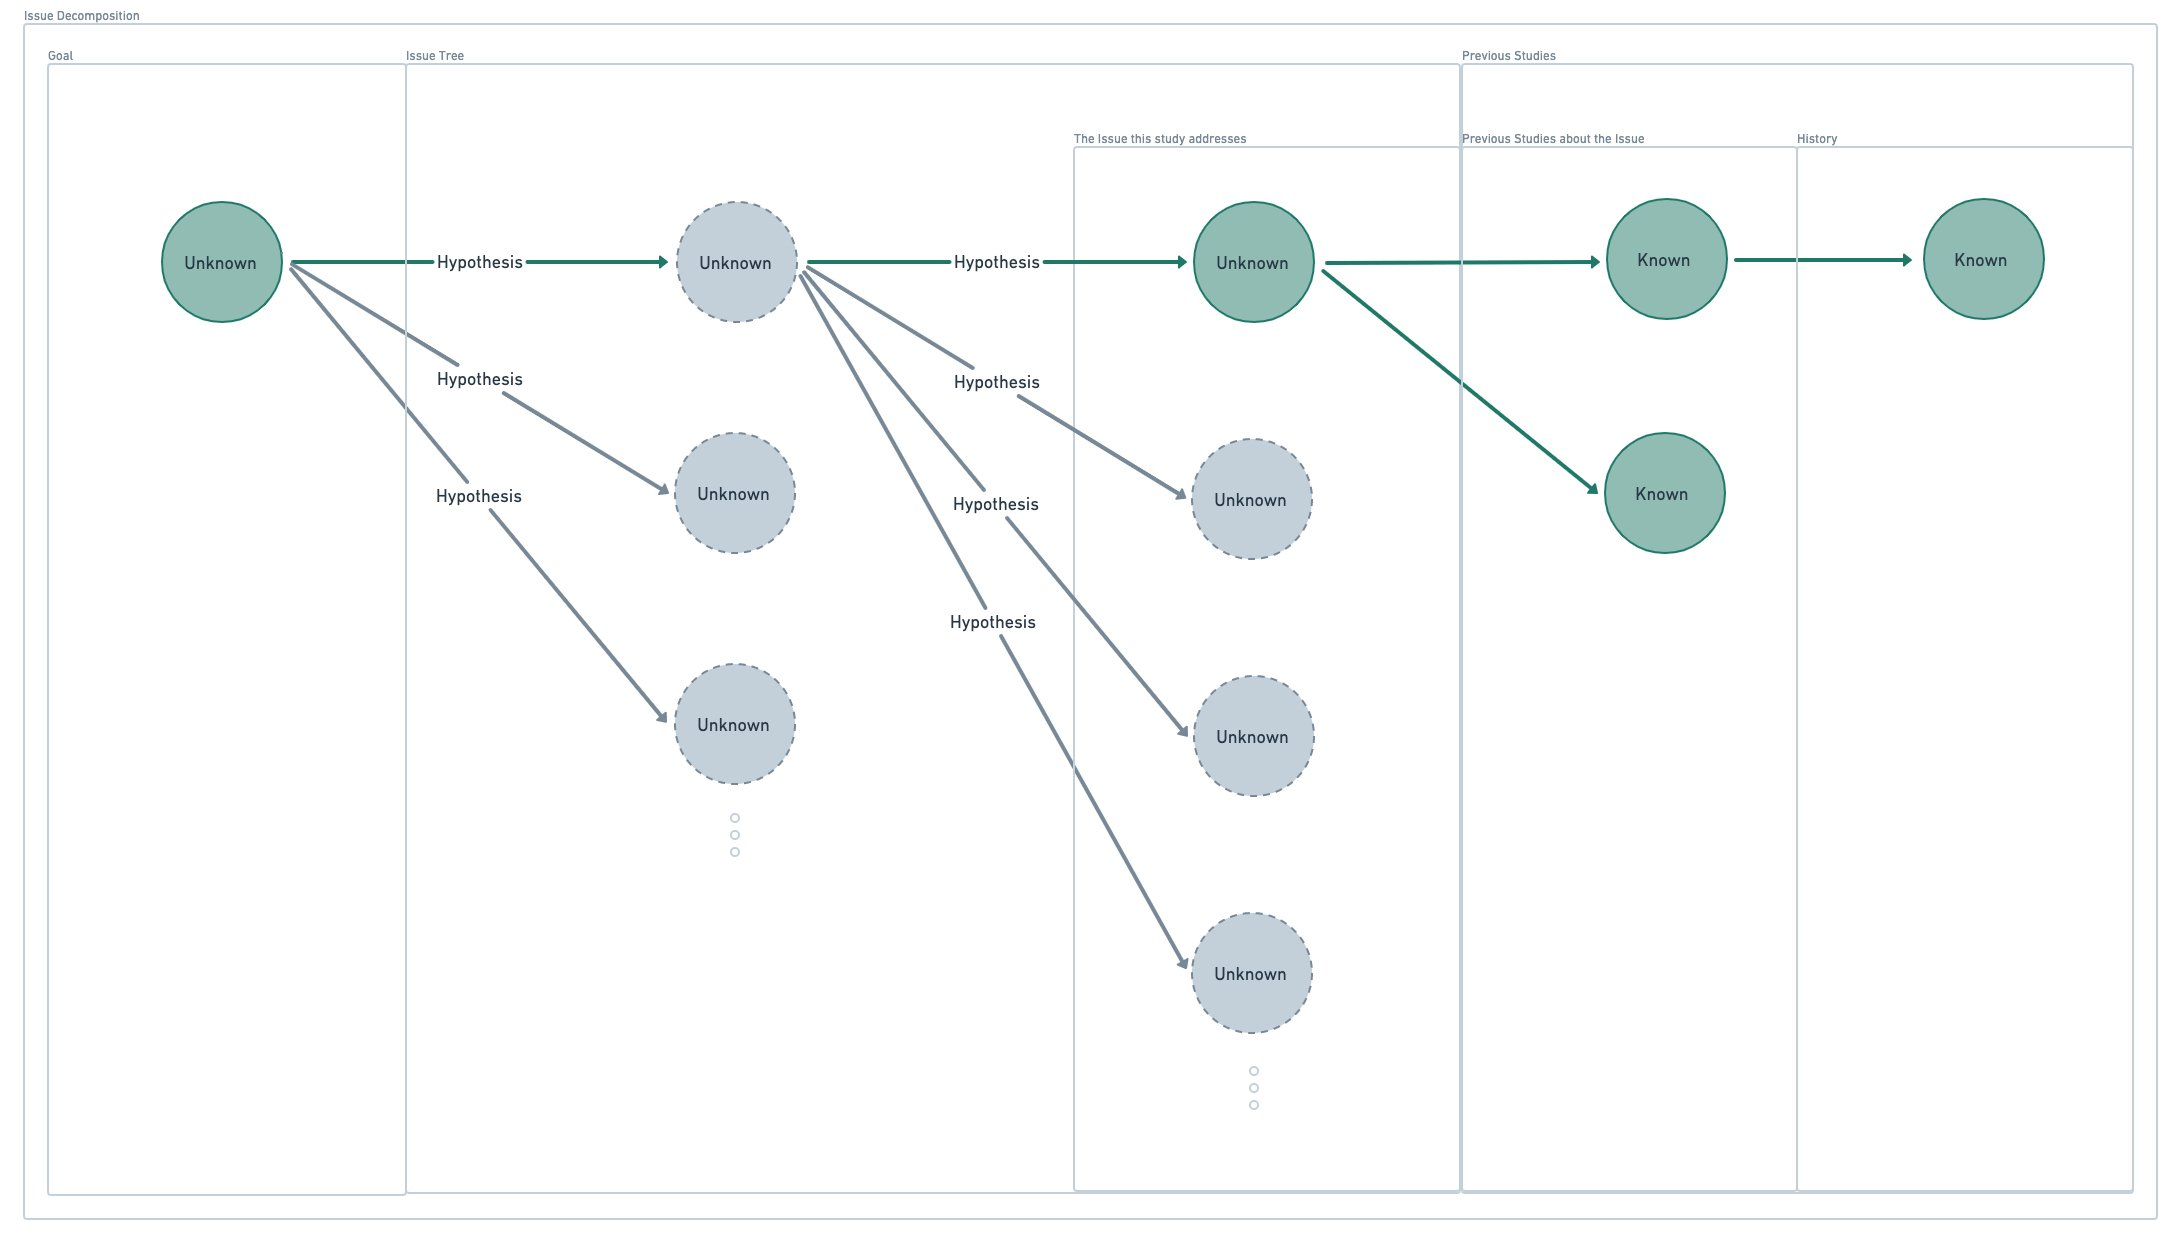
\includegraphics[width=\textwidth]{figs/unknown_tree.jpeg}
%     \caption{Caption}
%     \label{fig:unknown_tree}
% \end{figure}

% Several things are happening here. Firstly, listing the elements necessary for achieving the goal means generating sub-goals from the main goal. However, it's always a challenging problem to evaluate how a particular sub-goal contributes to the achievement of a given goal. Especially in the case of research, the target might be an too general and ambitious vision that nobody has achieved before, so I need to think about what needs to be done to break it down into appropriate sub-problems. In other words, it is necessary to construct a tree with nodes representing sub-goals. Namely, this is the tree of repetition of constructing a question and generating multiple hypotheses without verification. I will delve into the discussion of hypothesis generation in the next chapter, so I won't go into the details here.

% Secondly, it is necessary to identify the most important and feasible sub-goal from the selected candidate sub-goals. This is because only one question can be addressed in the end. However, assessing and comparing sub-goals is a challenging task since I have no experience to realize the ultimate goal and so have no data what sub-goal actually is the most important.

% Thirdly, the question to ultimately arrive at must be verifiable. If the question is not specific, meaningful verification cannot be performed. Overly broad or ambiguous questions can result in countless or trivial answers, or they may be too unclear to provide practical answers. Increasing the specificity of the question corresponds to deepening the depth of the sub-goal tree, so it may be important to construct a sufficiently deep tree and find an efficient way to navigate it. The verifiability is constrained by the knowledge, resources, such as funding and technology, that I currently have. Therefore, when conducting verification in reality, it is necessary to consider such feasibility. Whether to tackle a question with high feasibility or to further divide it into more sub-tasks for its realization is a matter of judgment. In any case, it is necessary to appropriately evaluate such feasibility. The scope of feasibility is vast, so it is a challenging problem to determine how to consider it in creating intelligent systems.

% In this discussion, I considered the method of outputting questions from the goal through the construction and exploration of a tree structure. However, as mentioned by the predecessors, if an end-to-end approach ultimately becomes a powerful method, it may be more desirable to consider a direction in which questions are directly output from the goal. In particular, even when performing multi-step reasoning, it seems more natural to improve reasoning abilities using the recently developed approaches to multi-step logical reasoning, rather than explicitly considering tree structures. 

% To pursue this direction in research automation, specifically, it may be worth considering the construction of higher-quality datasets for goals and research questions. For example, it may be possible to construct a dataset by extracting only the ultimate goal and the research questions actually solved from the introductions of papers. However, an important point to note here is that the research questions created by humans so far are not necessarily optimal for achieving research goals. Firstly, machines may be capable of maximizing the objective better than humans due to cognitive constraints. Secondly, not all human research has been conducted by working backward from a clear goal. Some studies were conducted simply because they seemed interesting while reading papers. In this regard, simply learning from human data may constrain the potential capabilities that machines can possess. Therefore, it becomes important to consider how to formulate the maximization of the probability of achieving research goals as a problem, rather than naive imitation learning of human data.

% As evident from the formulation, to construct research questions for contributing to achieve a specific goal, we need to solve long range reasoning problems. This problem is widely studied in machine learning research community to improve the reasoning capabilities of machine learning models and on generate intermediate goals in reinforcement learning. If these research fields produce significant results, they can be directly applied. In this sense, it might be beneficial to seek cooperation from those who are actively conducting research in these areas. One of the unique aspects of long-distance reasoning problems in research automation is that the goal is something that has never been achieved before. This means that you cannot naively learn from data and need to generalize out of distribution. Therefore, it's essential to acquire skills not just to recognize patterns but to properly trace the path of reasoning. Moreover, because the goal has not been realized, sub-goals and the paths that connect them are ultimately based on the accumulation of hypothesis generation. In this sense, it can be said that this is a highly uncertain inference. This implies that the choice of which node to select is far from self-evident compared to other logical reasoning problems. Furthermore, there is the issue of the complexity of the distance between the goal and the question, which is far more intricate than, for example, games or planning everyday trips. For instance, to truly achieve the goal, it may be necessary to build large-scale apparatus like particle accelerators from scratch. This also means that the temporal distance between the goal and the current location is very long. Therefore, it becomes a problem that feedback on how much solving the question contributed to the goal is significantly delayed. While we've only listed a few examples here, there may be other unique challenges and issues that become more serious in research. It will be necessary to work on refining these technical challenges into specific research tasks through discussions with researchers in reasoning and planning.

% \subsubsection{Important but Unnoticed Questions}

% One example of a ``good'' question seems to be one that, in its construction itself, brings benefits to many researchers. By considering why hypotheses regarding the question are unknown, it becomes somewhat clearer what kind of question this is.

% The reasons why the answer to a question remains unknown are diverse. In some cases, the question is simply new, and no one has had the time to come up with an answer yet. For instance, a question about the internet posed on the day it was invented may still remain unanswered because it has only been a day since its birth, and no one may have delved into it yet. In other cases, the question might simply not interest anyone, leading to an absence of answers despite the availability of time. This is an example of a question that remains unanswered because nobody is willing to tackle it, even though time exists.

% Furthermore, there are questions that are difficult, and no one has been able to solve them. For instance, the question of how to achieve human immortality has been contemplated by many, but due to its complexity, no answer has been found yet. Lastly, there are questions that are important for a particular purpose but remain unnoticed by everyone. As previously mentioned, realizing challenging objectives that are yet to be achieved poses difficult problems. In such cases, it is often unclear what is not known or what is at the heart of the problem. In such situations, clarifying the question itself holds great significance.

% Thus, constructing questions of this kind seems to be important as it can help shed light on the unknown. With this in mind, it appears worthwhile to discuss this topic in detail.\footnote{
% Please note that the concept of a question being unnoticed and the answer to the question being unknown are different. The necessary condition for research is that the answer to the question is unknown. 

% If the existence of a question is not known to anyone, then naturally, its answer would also be unknown since no one would have answered it. So, if the existence of a question is unknown, then the answer to the question is also unknown.
% }

% \textcolor{red}{TODO: Add discussion}

% \subsubsection{Diverse Good Questions}
% There have been various discussions on the elements that good research possesses. For example, \cite{hulley2007designing} proposed that good research question should satisfies FINER criteria (feasible, interesting, novel, ethical, and relevant) and \cite{alon2009choose} claims that a good problem is one that is most feasible and interesting to oneself.

% \textcolor{red}{TODO: Add more discussion on ``good'' questions, examples, discussion, what is good, what is important, specific question is good, etc.}
 

\subsection{Where Does a Question Come from?}
Research questions can arise in various situations. Some people may generate research questions as they logically think about how to achieve a goal. Others might come up with a question upon noticing some anomaly while observing experimental data. Furthermore, as with Kepler, one might realize that there might be something wrong with the underlying assumptions based on a discrepancy between results deduced from some assumptions and actual observational data. If one wants to create an AI that can autonomously construct research questions like humans, it seems necessary to develop an AI with a general methodology that can construct questions in any of these situations.

One of the challenges in trying to create such a general and autonomous research question constructor is determining how much input humans should provide to the AI and to what extent humans should design the mechanism for constructing questions. For example, the minimum input for an AI constructing questions for a goal is the goal itself. However, a goal might not be the minimum necessary input for other types of question generation methods. Also, as is often discussed in the context of research automation, if one aims to make the AI autonomously generate even goal itself, we would likely necessitate assuming even more primitive inputs for it, e.g. higher-level goal.

% For creating an autonomous system, the question construction module faces challenges due to being the initial building block of the system. This challenge is determining ``what should be the input to the question construction module.''

% Questions do not arise from nowhere. There is always something before reaching a question. In the example I mentioned earlier, for instance, the question may arise as a result of a literature review. Then, why did you conduct that literature review in the first place? It could be because there is a research theme you want to know about in the research field. And then why are you interested in that research theme? It could be because the topic of the first paper you encountered during graduate school was fascinating, or it could be because you have been interested in it since childhood. And there may be causes behind those as well.

% In this way, identifying where a question begins is a hard problem. If you think seriously about it, it will lead to an infinite regress. This is a significant problem when I want to realize an autonomous artificial researcher. As infinite regress can occur, the decision of where to terminate lies solely with the designer, and it is not automatically resolved by creating the system. Can I say that question construction is autonomous if the literature to read were given? Can I say that question construction is autonomous if research theme were given? I believe it is necessary to accumulate such discussions and determine how far to consider something as given, in order to define what qualifies as autonomous.

% In this paper, I assume that a trigger that requests a specific type of knowledge is given. And from there, it makes decisions about determining the unknown and constructing questions. The reason is that discovering questions with unknown answers is a necessary condition for research, and I believe this is the minimal requirement for it. However, one could also try to automate even the aspect of requesting a specific type of knowledge. The reasons for expecting the existence of certain knowledge can vary and are arbitrary. For example, I might have an objective and first consider what I need to do to achieve it. I then anticipate the necessary knowledge to accomplish those tasks. This corresponds to the demanding for a specific knowledge.

% As an another example, let's consider the case of a child asking, ``Why is the sky blue?'' In this case, the child may already have prior knowledge of the concept of ``sky'' and ``blue.'' Additionally, they may possess a naive concept of causality, believing that ``A is B, so there must be a reason for it.'' Thus, they may have expected to have the knowledge that ``the sky is blue because of B.'' However, when they reference their internal knowledge, they find that it does not contain the corresponding knowledge. Therefore, they may have asked the question ``Why is the sky blue?'' to evoke the knowledge they were lacking. In this case, the required knowledge is ``the sky is blue because of B.'' and this is induced just because the result of children combining known concepts.

% The question of ``why do I seek information'' has been extensively discussed in the context of curiosity. Indeed, as I proceed with the automation of these components, it becomes essential to delve into research on curiosity. Regarding this matter, I will touch upon the aspects mentioned in Chapter 3, if possible. 

\subsection{Types of Questions}

\subsubsection{``Why'' Question}

% Multiple Reasons for Unknownness

% new, unimportant, difficult, unnoticed, ... etc.

% This means that I distinguish between questions that are ``good'' and those that are not, based on certain criteria. 

% This means that I distinguish between questions that are ``important'' and those that are not, based on certain criteria. For example, \cite{alon2009choose} claims that a good question is one that solves challenges facing the research community. Likewise, I consider a question to be important if it generates knowledge that greatly contributes to a certain purpose. Valuing the degree of contribution to a purpose also implies viewing research as a form of problem-solving. \textcolor{red}{TODO: Add explanation of what this sentence means}

% Thus, in realizing an agent that autonomously constructs questions, it may become important to consider how to automatically determine ``goodness'' of the questions. To achieve this, it would be important to first understand in more detail what kind of questions I consider ``good''. \textcolor{red}{TODO: Add possible directions}

% \subsubsection{How to Practically Construct a Question}

% There has been much discussion on how to actually generate questions. Off course, these discussions primarily focus on how to formulate good questions. Therefore, please note that the examples mentioned here are proposals for generating such kind of questions.

% One typical approach to formulating a research question is to conduct a literature survey, identify research gaps in existing studies, and propose a question that aims to fill those gaps.

% \textcolor{red}{TODO: Add survey of how to construct questions; gap spotting, problemization, etc}

% Next, let's consider the process of constructing purpose-driven research questions. When aiming to conduct impactful research, I believe that constructing purpose-driven research questions is crucial. In this approach, I first set the ultimate objective. Then, I identify the most critical bottlenecks, or sub-goals, that are essential to achieving that objective. I once again consider sub-goals for these identified bottlenecks. This process is repeated, converging on more specific and feasible sub-goals that are of high importance. Finally, I frame the question to address these sub-goals as the research question. 

% In practice, I seem to determine the questions I should tackle in this way, implicitly and explicitly. For example, let's say that someone try to answer a question of ``How neural networks have reasoning capability?'' in his/her study. This question may come from a thought process of ``we want to create artificial general intelligence, which requires systematic thinking, that needs ...'' In this case, the final purpose is to achieve ``artificial general intelligence'', and the question addressed as a result is ``ow neural networks have reasoning capability?'' In other words, when I want to conduct important research, I follow a process that starts with the goal I want to achieve, considers the tree of important unknowns that should be clarified for its achievement, and sets the end of that tree as the research question. This process is summarized in Fig. \ref{fig:unknown_tree}.


% Of course, the purpose mentioned here may be a sub-goal of a higher-level goal. For example, the goal of ``creating general artificial intelligence'' may be a sub-goal of a more fundamental goal of ``satisfying intellectual curiosity,'' and the goal of ``satisfying intellectual curiosity'' may be biologically demanded for better exploration of the environment. These can lead to an infinite regression when considered strictly, so I won't delve into it any further here, but it could become an important issue when considering how to realize fully autonomous agent to construct questions.

% \subsubsection{Question}

% The construction of a question is the act of seeking information \cite{watson2015ask}. Specifically, in the context of research, I consider information as knowledge. The act of seeking knowledge involves two steps: 1. Recognizing the lack of knowledge and 2. Attempting to fill that knowledge gap. In this discussion, I assume that intelligence is designed to consistently generate questions when given input. Therefore, I temporarily set aside the aspect of "triggering action" related to the second step of attempting to fill the knowledge gap.

% The recognition of a knowledge gap occurs when I expect to have certain knowledge and, upon referencing my accessible knowledge, I find that it is not available. For example, when running a program and encountering an error that I cannot resolve on my own, I recognize that I lack the necessary knowledge.

% The reasons for expecting the existence of certain knowledge can vary and are arbitrary. In this case, I assume that a purpose given by a third party creates an expectation of certain knowledge. For example, in the case of humans, I first consider what I need to do to achieve a certain purpose. I then anticipate the necessary knowledge to accomplish those tasks, and when I find that it is not present within my existing knowledge, I recognize the knowledge gap.

% Lastly, in this discussion, knowledge refers to the collective body of research findings, particularly academic papers. In actual research, a researcher may personally have a question and then investigate previous studies to confirm that it is indeed unknown before formulating it as a research question. However, what is important in the construction of a research question is that it is unknown to other entities. Therefore, for simplicity, I directly refer to the entirety of academic papers without including the step of comparing personal knowledge.

% To summarize, to create an intelligence capable of constructing questions in this setting, I need to design it to expect the necessary knowledge to achieve a given purpose provided by a third party, search for that knowledge in academic papers, assess whether the papers contain sufficient knowledge to achieve the purpose, and express any knowledge gaps as questions.

% In this case, I excluded the discussion of triggering action by design. However, when considering increasing autonomy, it is important to discuss how to incorporate this aspect into learning and acquisition. The question of "why do I seek information" has been extensively discussed in the context of curiosity.

% Furthermore, in this case, I defined the expectation of knowledge as aiming to achieve a given purpose. However, as mentioned earlier, this does not affect the formulation of questions. For example, let's consider the case of a child asking, ``Why is the sky blue?'' In this case, the child may already have prior knowledge of the concept of ``sky'' and ``blue.'' Additionally, they may possess a naive concept of causality, believing that ``A is B, so there must be a reason for it.'' Thus, they may have expected to have the knowledge that ``the sky is blue because of B.'' However, when they reference their internal knowledge, they find that it does not contain the corresponding knowledge. Therefore, they may have asked the question ``Why is the sky blue?'' to evoke the knowledge they were lacking.

% In this way, the reasons for expecting the existence of certain knowledge can vary, and what, why, and how I seek information (knowledge) are not constrained by specific conditions. Therefore, when attempting to create an intelligence capable of constructing questions in the future, it is feasible to develop a more flexible intelligence.

% Additionally, in this case, I assumed that the given purpose and its achievement are predefined goals. However, humans naturally set their own goals. When considering the design of a more autonomous intelligence, it is conceivable to aim for automation in this aspect as well. However, as mentioned earlier, the question of what I seek knowledge about is not specific to research. Therefore

% , I temporarily set it aside for now. If I were to pursue this direction further, it would ultimately lead to an infinite regress, raising the question of how much information to consider as given.


%%%%%%%%%%%%%%%%%% Rearangement %%%%%%%%%%%%%%%%%%%%%%%%%%%%

% \subsection{question construction}
% Research is an endeavor to bring the unknown closer to the known. Therefore, it is necessary to first determine what unknown I aim to make known. And this unknown often takes the form of questions. For example, ``Why do deep neural networks with a large number of parameters generalize well?'', ``How can I prevent the problem of vanishing gradients?'', and like these. These are commonly referred to as \textit{research questions} or \textit{research problems}. Therefore, in this paper, I will refer to the step of determining this unknown as \textit{question construction}.

% \textcolor{red}{TODO: should describe question construction itself first. What is research question or research problem?}

% \subsubsection{Unknownness}
% As I have reiterated, it is a necessary condition for research that the answer to a question is unknown, or in other words, that there is a high degree of uncertainty. Therefore, it is essential in research to have methods that ensure the answer to a posed question is truly unknown, or to formulate questions that truly have unknown answers.

% Knowledge for humanity is primarily disseminated through research outcomes. Therefore, when examining all the research outcomes that have been generated thus far and finding that none of them provide an answer to a specific question, it seems reasonable to conclude that the question possesses sufficient uncertainty to warrant further investigation as a research endeavor. In particular, humanity has developed the culture to preserve the research outcomes in the form of papers. Therefore, it seems feasible to assess the unknown nature of an inquiry by examining all academic papers. However, it is impossible to review them all due to constraints in terms of time, technology, and cognitive limitations. Therefore, it is realistic to consider a question as unknown if it has been sufficiently and comprehensively explored through an extensive examination of these academic papers. In practice, I conduct literature reviews to synthesize existing research, identify research gaps in existing studies, and thereby ascertain the unknowness of my own questions or construct question for which the answers are unknown \cite{schryen2015theory}. \textcolor{red}{TODO: Consider where I will explain about literature review}

% % In the previous statement, it was mentioned that as long as the unknown is truly unknown and it can be approached towards becoming known, there should be no problem. The process of approaching the known will be explained in the next section, and here I will delve a bit more into the determination of unknownness. 

% However, in reality, such rigorous literature research is not always conducted in every case. Currently, researchers often demonstrate the unknownness of the answer to the question by referencing only a few related works and explaining that none of them have yet resolved the unknown. And when the paper is evaluated by reviewers, who are a small group of experts, if it is determined that the question has indeed not been answered so far, the provisional recognition of the unknown nature of the question is granted. This means that a subjective evaluation criterion is being used, where researchers and a small number of reviewers consider a question as unknown when none of their known studies provide an answer.

% % This implies the use of subjective evaluation criteria, where researchers examine several papers considered ``major literature'' in a field and consider them as unknown if none of them have provided an answer. Furthermore, as mentioned later, I evaluate the quality of research outcomes by having them assessed by a small number of experts in the same field. If these researchers determine that the previous studies have been sufficiently comprehensive, the determination of unknownness is considered somewhat valid. In other words, ultimately, the evaluation by a few experts may serve as the basis for establishing the unknownness.

% This current convention stems from the cognitive constraint that there is a limit to the literature that humans can examine. Since unknownness is a fundamental aspect of research, ideally, it should be evaluated objectively and rigorously. For instance, it would be desirable to quantitatively state which journals, what types of papers, and how many have been examined, and the result indicating their unknownness. Although systematic reviews already employ such approaches, there is, of course, a limit to the number of papers that can be evaluated manually and selection biases cannot be removed. \textcolor{red}{TODO: Add the explanation of systematic review, problems of it, and how AI can mitigate them.}


% However, I have not found a unified consensus on the definition of good question. but 

% \subsubsection{Questioning as Information Seeking Behavior}
% \textcolor{red}{TODO: Reconstruct}

% The construction of a question is the act of seeking information \cite{watson2015ask}. Specifically, in the context of research, I consider information as knowledge. The act of seeking knowledge involves two steps: 1. Recognizing the lack of knowledge and 2. Attempting to fill that knowledge gap. In this discussion, I assume that intelligence is designed to consistently generate questions when given input. Therefore, I temporarily set aside the aspect of "triggering action" related to the second step of attempting to fill the knowledge gap.

% The recognition of a knowledge gap occurs when I expect to have certain knowledge and, upon referencing my accessible knowledge, I find that it is not available. For example, when running a program and encountering an error that I cannot resolve on my own, I recognize that I lack the necessary knowledge.

% The reasons for expecting the existence of certain knowledge can vary and are arbitrary. In this case, I assume that a purpose given by a third party creates an expectation of certain knowledge. For example, in the case of humans, I first consider what I need to do to achieve a certain purpose. I then anticipate the necessary knowledge to accomplish those tasks, and when I find that it is not present within my existing knowledge, I recognize the knowledge gap.

% Lastly, in this discussion, knowledge refers to the collective body of research findings, particularly academic papers. In actual research, a researcher may personally have a question and then investigate previous studies to confirm that it is indeed unknown before formulating it as a research question. However, what is important in the construction of a research question is that it is unknown to other entities. Therefore, for simplicity, I directly refer to the entirety of academic papers without including the step of comparing personal knowledge.

% To summarize, to create an intelligence capable of constructing questions in this setting, I need to design it to expect the necessary knowledge to achieve a given purpose provided by a third party, search for that knowledge in academic papers, assess whether the papers contain sufficient knowledge to achieve the purpose, and express any knowledge gaps as questions.

% \begin{figure}[htb]
%     \centering
%     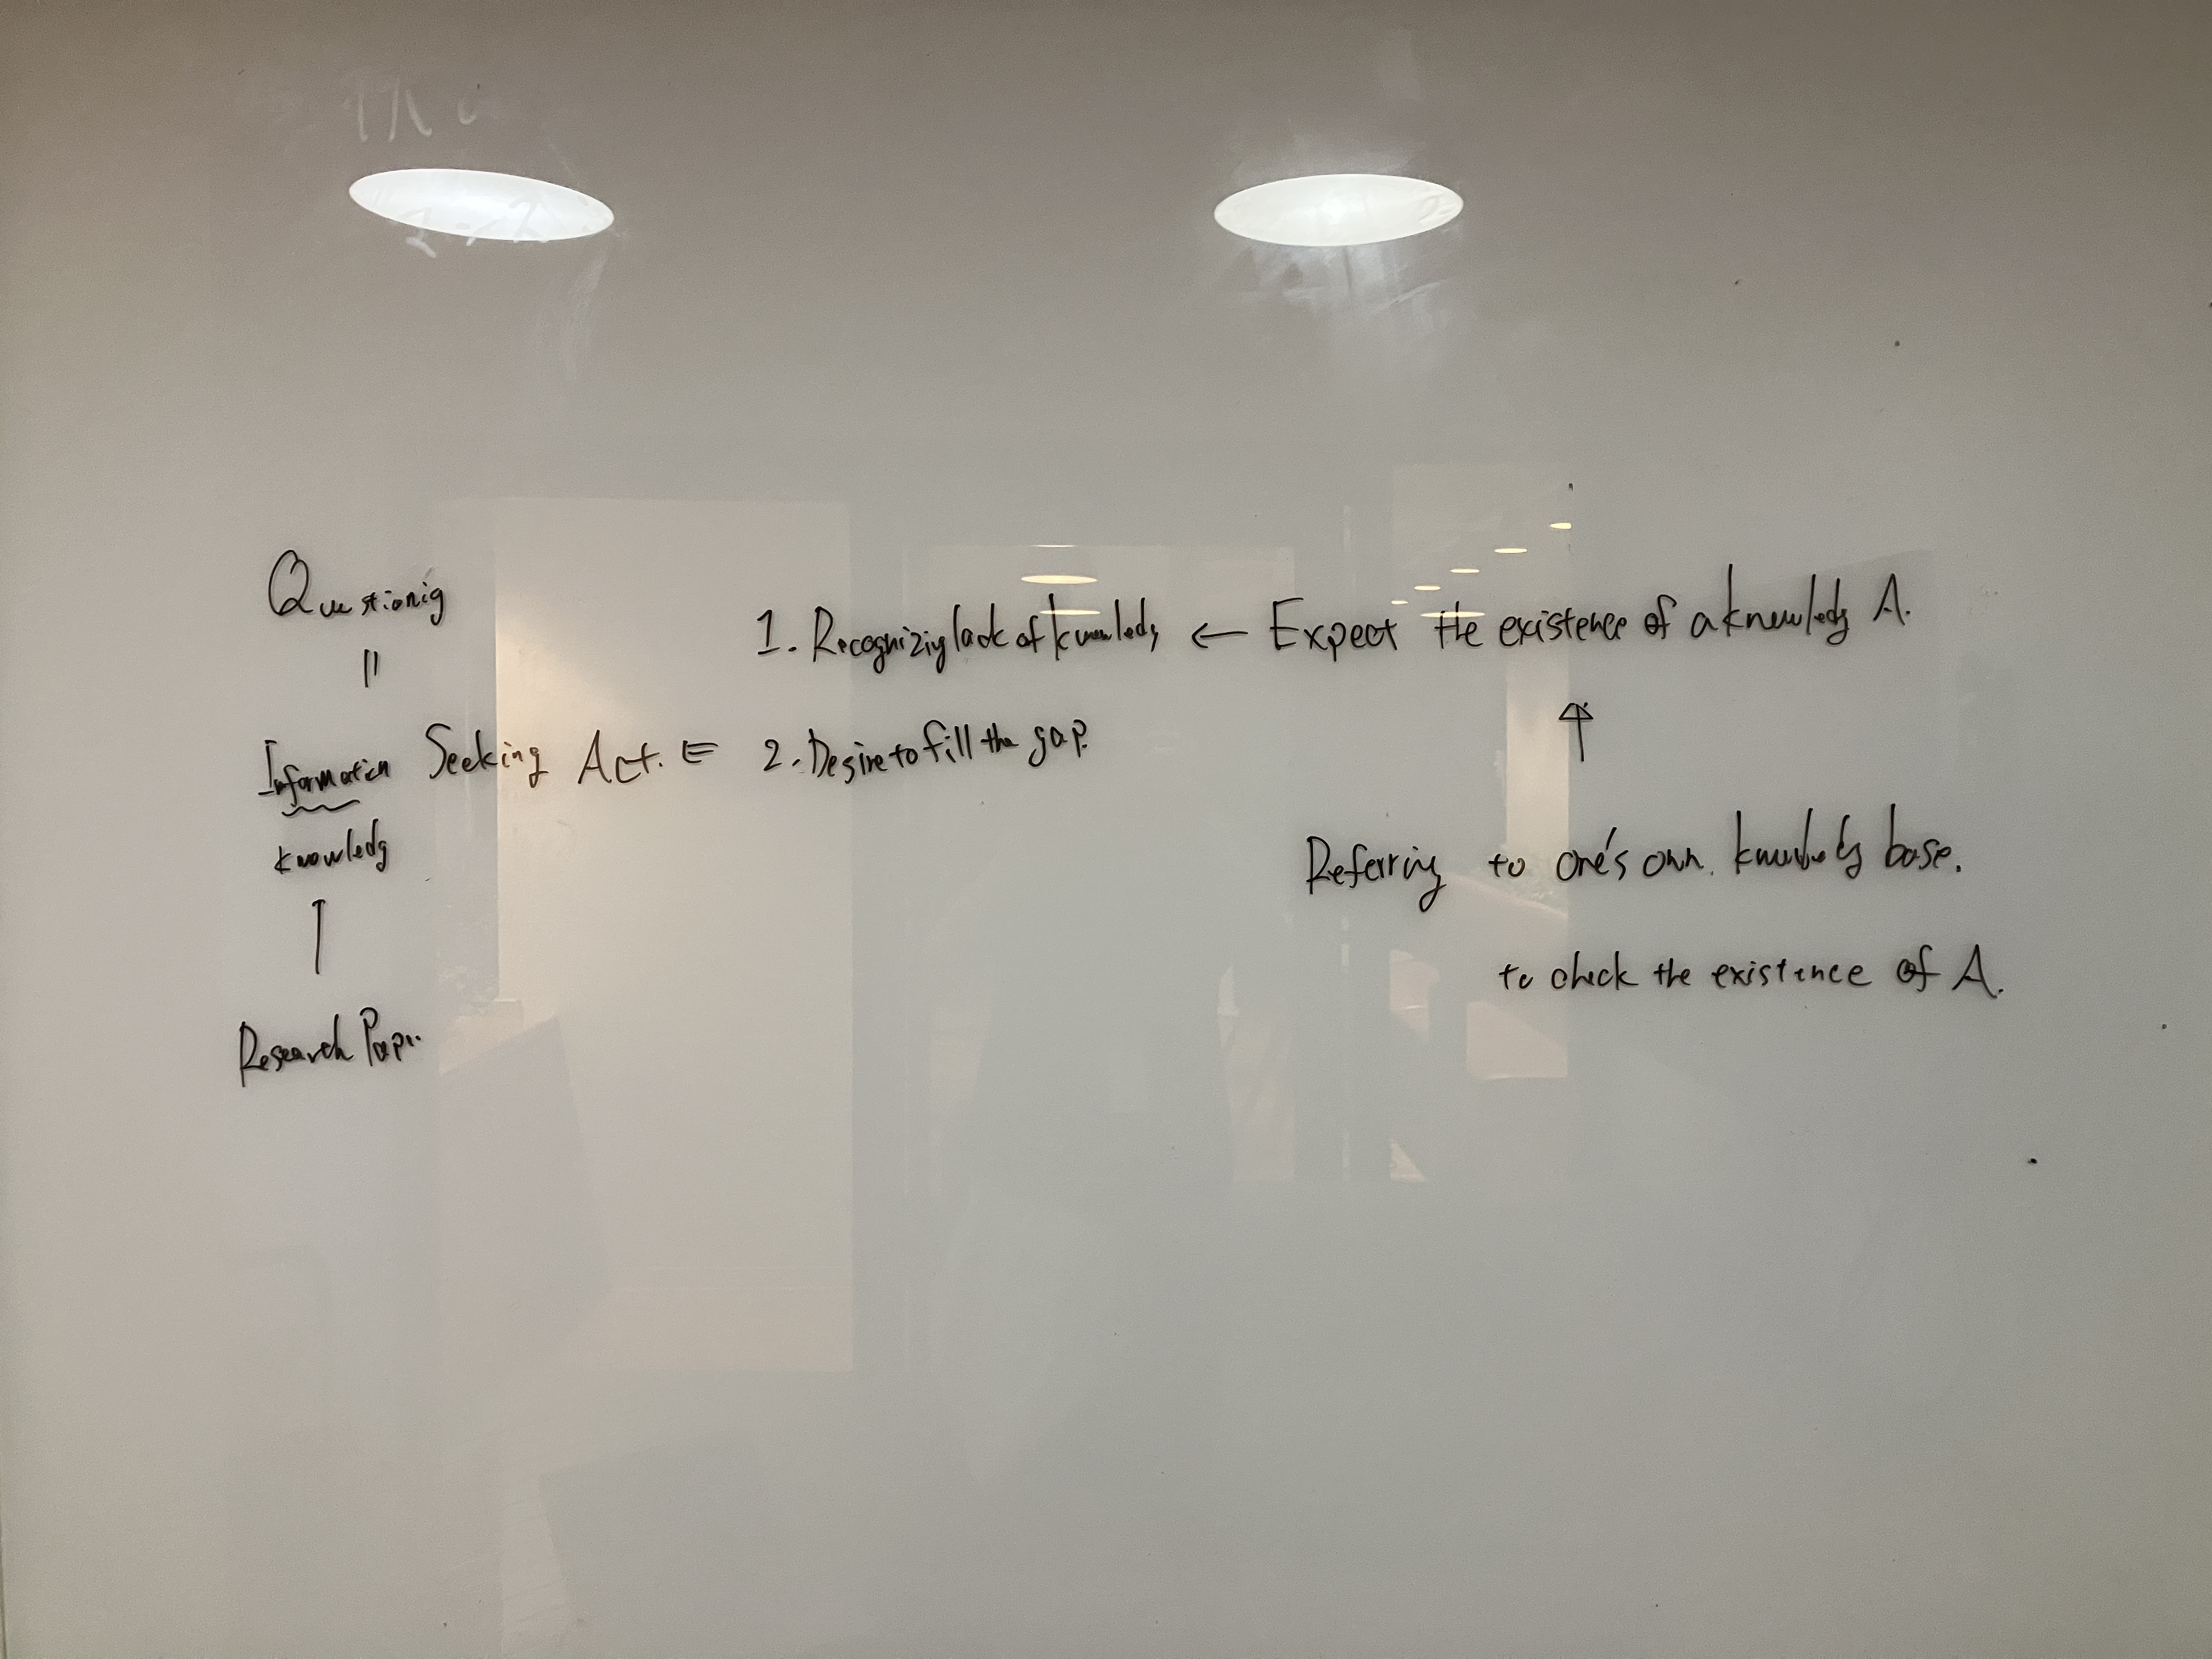
\includegraphics[width=\textwidth]{figs/question_formulation.jpg}
%     \caption{question construction}
%     \label{fig:enter-label}
% \end{figure}

% \textcolor{red}{TODO: Is question construction information retrieval??}


% Asking questions is an act of seeking information \cite{watson2015ask}. The act of seeking information (or knowledge) arises from realizing the lack of one's own knowledge and the desire to fill that gap. Therefore, to create intelligence that can autonomously ask questions, it is necessary to incorporate mechanisms that induce these behaviors.

% Determining what triggers this behavior in humans is a challenging problem. However, when designing a system, it is sufficient if it can induce such behavior, regardless of what it actually is. The principle that ``behavior is triggered when it is somehow desirable for the agent'' represents this idea. You are probably familiar with this concept in reinforcement learning, where rewards (desirability of actions) are provided, and maximizing the expected value of these rewards is formulated as an appropriate way to induce behavior.

% The notion of triggering behavior by realizing the lack of one's own knowledge and attempting to fill it has been extensively studied in the context of curiosity in the field of reinforcement learning. In research, agents that pose questions can generally be formulated within this framework.

% \subsection{question construction}
% The construction of a question is the act of seeking information \cite{watson2015ask}. Specifically, in the context of research, I consider information as knowledge. The act of seeking knowledge involves two steps: 1. Recognizing the lack of knowledge and 2. Attempting to fill that knowledge gap. In this discussion, I assume that intelligence is designed to consistently generate questions when given input. Therefore, I temporarily set aside the aspect of "triggering action" related to the second step of attempting to fill the knowledge gap.

% The recognition of a knowledge gap occurs when I expect to have certain knowledge and, upon referencing my accessible knowledge, I find that it is not available. For example, when running a program and encountering an error that I cannot resolve on my own, I recognize that I lack the necessary knowledge.

% The reasons for expecting the existence of certain knowledge can vary and are arbitrary. In this case, I assume that a purpose given by a third party creates an expectation of certain knowledge. For example, in the case of humans, I first consider what I need to do to achieve a certain purpose. I then anticipate the necessary knowledge to accomplish those tasks, and when I find that it is not present within my existing knowledge, I recognize the knowledge gap.

% Lastly, in this discussion, knowledge refers to the collective body of research findings, particularly academic papers. In actual research, a researcher may personally have a question and then investigate previous studies to confirm that it is indeed unknown before formulating it as a research question. However, what is important in the construction of a research question is that it is unknown to other entities. Therefore, for simplicity, I directly refer to the entirety of academic papers without including the step of comparing personal knowledge.

% To summarize, to create an intelligence capable of constructing questions in this setting, I need to design it to expect the necessary knowledge to achieve a given purpose provided by a third party, search for that knowledge in academic papers, assess whether the papers contain sufficient knowledge to achieve the purpose, and express any knowledge gaps as questions.

% In this case, I excluded the discussion of triggering action by design. However, when considering increasing autonomy, it is important to discuss how to incorporate this aspect into learning and acquisition. The question of "why do I seek information" has been extensively discussed in the context of curiosity.

% Furthermore, in this case, I defined the expectation of knowledge as aiming to achieve a given purpose. However, as mentioned earlier, this does not affect the formulation of questions. For example, let's consider the case of a child asking, ``Why is the sky blue?'' In this case, the child may already have prior knowledge of the concept of ``sky'' and ``blue.'' Additionally, they may possess a naive concept of causality, believing that ``A is B, so there must be a reason for it.'' Thus, they may have expected to have the knowledge that ``the sky is blue because of B.'' However, when they reference their internal knowledge, they find that it does not contain the corresponding knowledge. Therefore, they may have asked the question ``Why is the sky blue?'' to evoke the knowledge they were lacking.

% In this way, the reasons for expecting the existence of certain knowledge can vary, and what, why, and how I seek information (knowledge) are not constrained by specific conditions. Therefore, when attempting to create an intelligence capable of constructing questions in the future, it is feasible to develop a more flexible intelligence.

% Additionally, in this case, I assumed that the given purpose and its achievement are predefined goals. However, humans naturally set their own goals. When considering the design of a more autonomous intelligence, it is conceivable to aim for automation in this aspect as well. However, as mentioned earlier, the question of what I seek knowledge about is not specific to research. Therefore

% , I temporarily set it aside for now. If I were to pursue this direction further, it would ultimately lead to an infinite regress, raising the question of how much information to consider as given.

% \begin{figure}[htb]
%     \centering
%     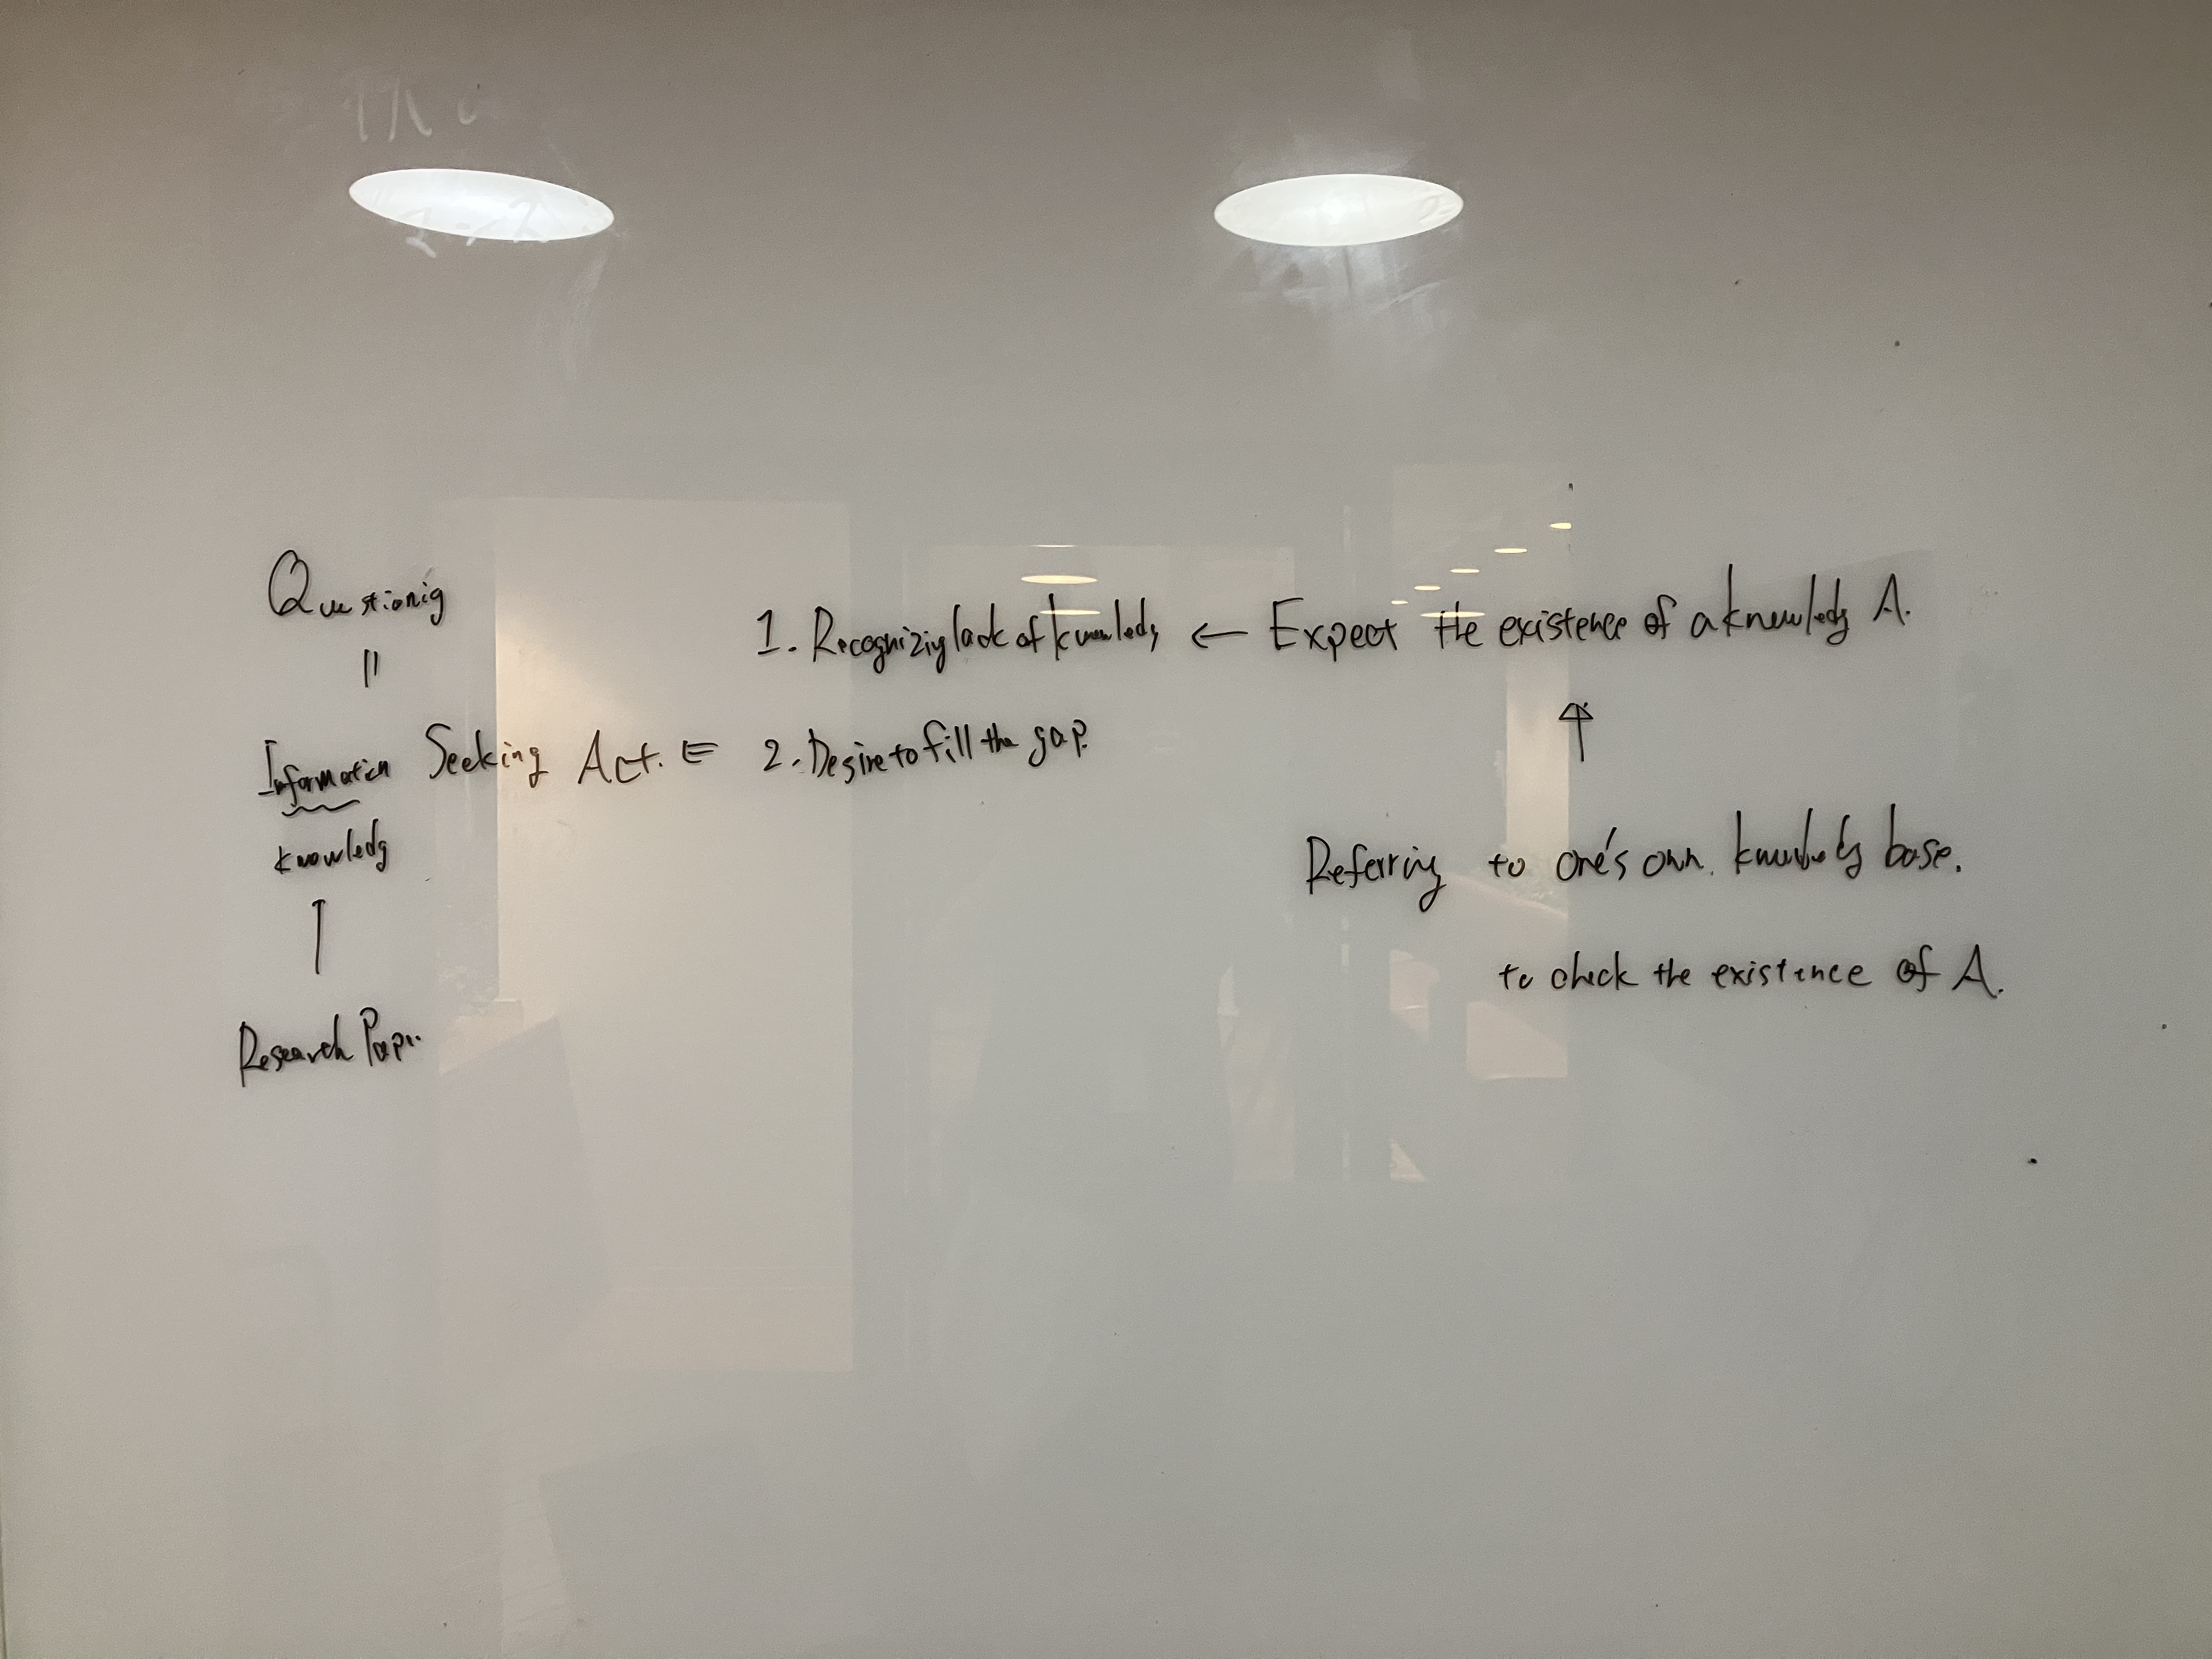
\includegraphics[width=\textwidth]{figs/question_formulation.jpg}
%     \caption{question construction}
%     \label{fig:enter-label}
% \end{figure}


% \textcolor{red}{TODO: Is question construction information retrieval??}


% \subsection{Conclusion}

% \begin{enumerate}
%     \item Determing the existence of expected knowledge:
%     \begin{enumerate}
%         \item Searching for knowledge directly related to the expected knowledge.
%         \item Determining whether the knowledge has been properly validated.
%     \end{enumerate}
% \end{enumerate}

% 1.b is specific to the automation of research. 





% I have listed what I believe are important elements in the construction of questions. However, these are considered important under the assumptions mentioned earlier. For instance, if the goal is not to acquire knowledge necessary for achieving an objective, but to generate knowledge that an individual finds interesting, the necessary elements in question construction (particularly in parts 1.a and 1.b) would change. As previously mentioned, the value of knowledge is determined in relation to context and there's a high degree of uncertainty about how the value of knowledge will evolve in the future. This makes it fundamentally important to have a diverse range of ways to generate questions. The object achievement is highly prevalent and is expected to produce ``important'' knowledge, which is why it is discussed here. However, it is important to discuss what other ways of formulating questions could exist and how they can be implemented.

\section{Hypothesis Generation}
I began by explaining that I first formulate the unknown I am addressing in the form of a question. The process of finding answers to this question is research. Here, because the answer to this question is, of course, unknown, it requires inference as to what the answer could be. As a result of this inference, a plausible answer is formulated. This process corresponds to the \textit{hypothesis generation}. Hypothesis generation is the inference about the unknown and the definition of research is to transform unknown to known. Thus, every research including deductive research must entail hypothesis generation implicitly or explicitly. In this sense, hypothesis generation should be the second module of knowledge production system.

The belief that a hypothesis is true is the very object that can become knowledge in response to a question. If a hypothesis withstands proper testing, the belief in its plausibility strengthens. Conversely, if a hypothesis does not withstand testing, that belief is weakened. Therefore, the former generates knowledge that ``the answer to question A is hypothesis B,'' while the latter generates knowledge that ``the answer to question A is not hypothesis B.'' 

Hypothesis generation is the act of creating potential answers to a question, so naturally, it is essential to generate plausible hypotheses that are close to the actual answer. Therefore, let's start by referring to how humans generate hypotheses and then discuss how I can generate reliable hypotheses, drawing inspiration from human methods.

\subsection{Generating Plausible Hypothesis}
% \subsection{Hypothesis Generation: Proposal}
% As mentioned earlier, from the perspective of knowledge production, I believe that hypotheses are sufficient in principle if they fulfill the function of providing provisional answers to questions. However, in order to avoid unnecessary testing, it is important to derive ``plausible'' hypotheses. There are various approaches to this, but to provide some food for thought, I would like to share my personal view on how humans generate hypotheses.

Hypothesis generation is sometimes considered an unanalyzable, emergent process or a result of genius.\footnote{
Since 19th centuries, the act of producing knowledge, in particular hypothesis, and that of verification of it have been distinguished as the context of discovery and context of justification \cite{sep-scientific-discovery}. And during the most of the 20th centuries, the discovery caught much less attention by philosophers of science.

In engineering discussions, there is often explicit formulation of sets or candidates of hypotheses, and the discovery of hypotheses in such situations is often discussed \cite{simon1973does,kitano2021nobel,bengio2022ml4sci}. However, when automating hypothesis generation it is also important to consider how such candidates arise in the first place. There have been attempts to understand this process, such as highlighting the importance of analogy \cite{thagard1984conceptual} or mental model \cite{nersessian1999model}, but the question of how to generate ``good'' hypotheses still remains unanswered. The generation of initial hypothesis candidates has been discussed in the context of creativity in science. As you are well aware, however, current machine learning models are already capable of executing creative tasks effectively \cite{sep-creativity}. Thus, there is a debate about how much emphasis should be placed on creativity when considering the development of artificial intelligence capable of generating new hypotheses.
} However, I believe that human-generated hypotheses are produced through a process of trial and error in rational inference. In the following discussion, for the sake of simplicity, I will focus on hypothesis generation for why questions.\footnote{
Please note that not all research questions are why questions (e.g., ``Does life exist beyond Earth?'' is not a why question, but it is a scientifically investigable question).
}

% \subsection{Plausible Hypothesis and Unknownness}

% While predictions that are highly unlikely to be confirmed, such as random guesses, can still qualify as research, they do not contribute much knowledge because they are expected to be easily rejected without undergoing rigorous testing. It becomes a waste of resources to invest in validating such predictions. Therefore, it seems to be crucial for ``meaningful'' research to propose hypotheses that are somewhat plausible.

% It is immediately evident that this is a non-trivial problem. This is because research, despite being an endeavor to answer unanswered questions, requires considering plausible candidate answers for those questions. Here, if the unknown under investigation is entirely unrelated to existing knowledge, it is impossible to make meaningful predictions about it. This is because predictions are based on experiences and data. In other words, high novelty and high uncertainty indicate a complex structure that cannot be immediately predicted from past knowledge and experiences. It implies that constructing plausible hypotheses necessitates the ability to discern these complex structures and patterns from past experiences. While it is difficult to determine what is unknown and what constitutes a complex structure, these can be crucial points to consider when advancing the automation of research.

\subsubsection{Analyzing Question}
Researchers start with a question, the composition of which has been discussed in the previous section. Given the question, I break down the content of the question and analyze each part in detail. For example, let's say I have a question, ``Why are apples red?'' The first thing I would consider is what an apple is and what red means. I would also think about what it means for something to be red. Then, I focus on the properties of apples and the color red and abstract them. I may also think about other red things besides apples. If I already know the reason why tomatoes are red before knowing why apples are red, I might consider that the reason for tomatoes being red could apply to apples as well. By conducting this kind of analysis, I can connect my understanding to existing similar knowledge and attempt to explain using those existing reasons. These ways of focusing on abstract structural similarities between specific concepts and inferring that what can be said about A, which has the same structure, can also be said about B is called \textit{analogical reasoning}. This has been considered to be important method in hypothesis generation \cite{hesse1965models,thagard_1984,gentner1993shift,holyoak1996mental,dunbar1997scientists}.

For those simple examples given above, one can easily find analogical examples. However, many of the questions researchers actually grapple with are much more complex, and it's not immediately clear how they relate to existing knowledge. Even in such situations, researchers have managed to generate plausible hypotheses by analyzing research question thoroughly.

Such thorough analysis of questions seems particularly important when it comes to making significant discoveries that are remembered in history. Let's consider Charles Darwin as an example, who proposed the concept of natural selection. Darwin appears to have gone through a process of trial and error before arriving at the idea of natural selection \cite{gribbin2022origin}. After returning from his voyage on the HMS Beagle, he began to question how evolution occurs. It seems that he read the works of Lyell and Linnaeus, and particularly from Lyell's writings, he realized the importance of selection in evolution. The question then shifted to what could serve as a natural equivalent of artificial selection. Later, after reading Malthus' book on population, Darwin understood that in nature, competition leads to the preservation of advantageous species and the extinction of disadvantageous ones, which is the process of natural selection.

In essence, Darwin initially had the question of ``how does evolution occur,'' but through analyzing this question, referring to previous research, and conducting experimentations and observations, the question transformed into ``what is the equivalent of artificial selection in nature?.'' And it was through this transformation of the question that he was able to recognize the similarities between Malthus' discussion on human society and the mechanism he was seeking. Although the process is complex, this is the same as the hypothesis generation process I explained above in that he analyzed and transformed the question, finding analogies with existing knowledge and reaching a plausible hypothesis.

In the case of Darwin, it involved a more observational approach within the field of natural history, which prompted the transformation of his question. However, in fields such as theoretical research that utilize mathematics, different methods may be employed. For example, consider the scenario where there are two theories, theory A and theory B, and the goal is to achieve a unified description between them. In this case, one might repeatedly perform mathematical transformations on the objects described by each theory, reducing the significant problem of ``incompatibility between Theory A and Theory B'' to inconsistencies between specific properties of each theory. By introducing axioms that resolve these inconsistencies, it may be possible to construct a unified theory. It is important to reiterate that in cases where the subject matter is mathematically described, formal operations can be applied to objects of interest, such as object A and object B, to transform them into different forms. This process can lead to the discovery of unexpected similarities. It is through this approach that one can discuss the similarities between objects even when they may defy intuition or cannot be imagined through empirical means. 

Therefore, I believe that thorough analysis of question plays a powerful role in identifying similarities between objects, especially in cases where it is necessary to discuss the similarities between objects that may not be intuitively evident or imagined through experience. I believe that this is the core of the human hypothesis generation. The art of discovering structural similarities between two different objectives is called \textit{analogical reasoning}. This has been considered to be crucial for hypothesis generation \cite{hesse1965models,thagard_1984,gentner1993shift,holyoak1996mental,dunbar1997scientists,gentner2002analogy}. 

\subsubsection{Confirming Plausibility in Hypothesis Generation}

In the previous chapter, I explained how I transform questions by analyzing them and connecting them with existing knowledge. However, there seem to be countless ways to bring about changes in the questions. So, how exactly do I go about transforming the questions? Let's now describe the process of question transformation that I have in mind.

% In simple cases like ``apples are red,'' it may be sufficient to apply existing knowledge. However, in research, especially when tackling challenging questions, I believe that the following steps are involved. 

First, from the knowledge at hand, I select several hypotheses that are strongly related to the question and have a high level of confidence, and then proceed with accepting these hypotheses as premises. For example, the existing knowledge that tomatoes are red for reason A, strawberries are red for reason B  are strongly linked with the proposition that apples are red for reason C by the presence of the word ``red.'' Let's assume that I have a high level of confidence in the proposition that tomatoes are red for reason A, but only a low level of confidence in the proposition that strawberries are red for reason B. In this case, the reason A for tomatoes being red would be selected as the premise.\footnote{
In the case of humans, it may not always be the case that I prioritize knowledge with a high level of confidence. For example, let's consider a situation where I have recently read a book and acquired some highly impactful knowledge. In this scenario, even during the process of question analysis, I might be inclined to consider using this newly acquired knowledge because it has left a strong impression on us. This inclination is not solely based on its level of confidence, but rather because the knowledge has made a lasting impression, leading us to take it as a premise while analyzing the question. Like this, determining what knowledge humans choose to adopt as premises is a complex issue, and I refrain from delving into this issue in this paper.
}

Next, I will not focus on the parts of the question that pertain to the meaning of the premises or the deduced results that answer them. For example, going back to Darwin's example, when Darwin read Lyell's book, he took the proposition that ``selection matters in evolution'' as a premise. As a result, he left aside the question of ``what is important for evolution.'' Instead, he shifted his focus to solving the question of ``how does nature make selections?''

Once a certain premise is accepted, the next step involves examining the consistency between the consequences brought about by that assumption and one's existing knowledge. If introducing that premise does not lead to contradictions with strongly held beliefs, then the introduction of the premise is deemed acceptable. On the other hand, if introducing the premise results in contradictions with one's existing knowledge, it becomes a matter of choosing between the two. 

% This involves comparing the consequences brought about by the introduction of that premise with retaining one's existing knowledge and selecting the one that seems more favorable in some sense. For instance, Kepler compared the consequences of introducing the assumption of circular motion for planets with observational data and the results of his proofs, and eventually decided to discard the assumption of circular motion.

% or generating hypotheses that maintain consistency with this knowledge. Specifically, I generate hypotheses that seem relevant, and then verify that they do not contradict existing knowledge.

By considering the relationships between existing knowledge and new knowledge, and reevaluating which ones are deemed more plausible, one can undergo a process of transforming the question into its more essential form and generating plausible hypotheses. I seem to generate plausible hypothesis by transforming the question in like these steps.

\subsubsection{Continuity between Hypothesis Generation and Hypothesis Verification}

From the explanation so far, it becomes evident that in order to generate ``plausible'' hypotheses, I am conducting operations that involve changing my beliefs about the truth of those hypotheses. This seems natural since generating ``plausible'' hypotheses inherently involves such belief updates. However, this observation may offer significant insights into my current discussion. I define knowledge production as the updating of beliefs, which includes the construction of questions, the generation of hypotheses, and the operation I refer to as hypothesis testing, where I update my belief about whether a hypothesis is true. The implication of this discussion is that the process of generating ``plausible'' hypotheses and hypothesis testing share similarities. In reality, there are cases where hypothesis generation and justification are tightly connected in research practice \cite{arabatzis2006inextricability}. This leads to the question of whether I need to separate the processes of hypothesis generation and hypothesis testing.

However, I do not think that the fact that a single process play roles for both hypothesis generation and verification means that they are also play the same role for knowledge production. I believe that hypothesis generation and verification play two distinct role for knowledge production, and that's why I discuss separate them as two distinct modules.

You may say that it is not entirely implausible to interpret both hypothesis generation and verification as being ``belief updates.'' Certainly, this similarity becomes more evident, particularly when contemplating the generation of ``probable'' hypotheses. For instance, let's consider a scenario where belief values are continuous. In this case, generating a hypothesis involves changing the belief value of a certain hypothesis from its original value of, say, 0 to something like 0.1. Subsequently, if multiple hypothesis candidates are considered, and one is chosen as probable based on previous research, the belief in this hypothesis might increase to around 0.3. Through the final verification of this hypothesis, the belief might reach approximately 0.9, resulting in the formation of knowledge. From this perspective, hypothesis generation and verification can be seen as the process of modifying beliefs.

However, when aiming for knowledge production within a specific society, there is a distinction. During the verification phase, the beliefs that are updated are shared beliefs. In contrast, during the generation of probable hypotheses, the updating of shared beliefs is not required. Consequently, in the context of knowledge production, hypothesis generation generates beliefs that can be updated, while hypothesis verification serves as the means to update those beliefs, thus playing distinct roles.

% \subsection{Continuity between Hypothesis Generation and Verification}
% So far, I have emphasized that hypothesis generation and hypothesis testing are functionally distinct, and that seems somewhat reasonable. However, when considering the generation of "plausible" hypotheses, these boundaries become somewhat ambiguous.

% Since testing incurs costs, in reality, humans carefully choose hypotheses worthy of testing. Even after hypothesis testing is made more efficient by machines, narrowing down hypotheses to a certain extent remains practically essential. Therefore, this is a problem that persists even after knowledge generation is achieved through machines.

% When considering the generation of ``plausible'' hypotheses, it simply means strengthening the certainty about the truth or falsehood of a hypothesis. In other words, in terms of changing the belief about the truth or falsehood of a hypothesis, this can be seen as similar to testing. For example, in experimental research, I believe there is often a pilot study conducted before starting full-scale experiments. This is nothing more than evaluating whether the hypothesis is worth pursuing for rigorous testing.

% Therefore, it may be possible to identify hypothesis generation and hypothesis testing as being synonymous in the sense of belief updating. However, I still believe that there are differences between hypothesis generation and hypothesis testing. The confidence in hypothesis generation is ultimately a matter of individual researchers or those involved in the research, and it is not necessary for all members of society to share that confidence. On the other hand, testing requires methods that update the common beliefs of members of society. Therefore, while hypothesis generation and hypothesis testing can be regarded as equivalent in terms of belief updating, they may differ in the strength of that belief.

% Obviously it is not possible to consider the consistency for all possible knowledge, so in practice, researchers seem to be checking the consistency of the hypotheses with several studies or knowledge that they have in mind. The knowledge  may be the recent interesting papers they have read, knowledge they strongly believe in, and so on. The knowledge that comes to the researcher's mind at that moment and is prioritized in their thinking is likely to become the premises for these hypotheses. 

% In highly mathematicalized disciplines like physics, for example, one might judge the plausibility of a hypothesis by comparing the deduced consequences from that hypothesis with existing knowledge. In this way, hypotheses that are judged to be somewhat consistent with the assumed premises may be recognized as ``plausible'' and worthy of rigorous testing. Of course, there are factors other than the plausibility of a hypothesis that can affect its ``value,'' but I believe that plausibility is the most important value in terms of knowledge production.

\subsection{Hypothesis Generation from Verification Results}
So far, I have been discussing the process of generating hypotheses by analyzing a given question. In this case, the hypotheses are intended to answer the question from start to finish. However, in reality, I may end up generating hypotheses that are for completely different questions than the one I initially set out to solve. Surprisingly, some of these serendipitously generated hypotheses can become profoundly important and leave a mark in history. Let's take a moment to consider how such hypotheses are generated through this process.

Such hypotheses are born while attempting to identify the causes of verification results. Once a hypothesis is generated, the validity of it is assessed through hypothesis testing. In actual research practice, even if hypothesis testing yields negative results, it does not necessarily mean that the proposed hypothesis is completely discarded. Instead, supplementary premises may be introduced into the initially proposed hypothesis, and the modified hypothesis may be retested. On the other hand, it is also possible that the assumptions of the hypothesis are reconsidered, leading to the generation of new hypotheses. These are all practices of researchers involved in hypothesis generation, so let us explain them in more detail.

First, when humans think about something, they always need some assumptions. These assumptions refer to the knowledge or beliefs that individuals provisionally consider as ``correct.'' For example, when interpreting data at hand, one may assume that the measuring instrument used to generate the data is reliable, or that the principles of classical mechanics used for data collection are valid, or that the insights from several previous studies are valid. Additionally, researchers often introduce auxiliary hypotheses implicitly or explicitly during their investigations. For example, tentatively decided hyperparameters or auxiliary hypotheses introduced during calculations also become premises. Furthermore, there are implicit or explicit guiding principles and beliefs, such as the belief that ``hypotheses should be simple'' or that ``theories should be beautiful,'' which serve as premises for hypothesis derivation as well.

When verification yields negative results, all these assumptions, including the ones that are implicit, can be the cause for the result. The proposed main hypothesis itself may be incorrect, the auxiliary hypotheses may be incorrect, the observations may be incorrect, or all of them may be incorrect. Researchers must identify which of these possibilities is the cause. This is known as the problem of Duhem-Quine's thesis \cite{sep-scientific-underdetermination}. This is like trying to generate hypothesis on the question of ``What is the cause of the error?''. As you can understand, this is an extremely challenging problem since this is like debugging a system that is unstructured, where the entire code is not visible, and there is no systematic approach, and you have to grope in the dark. 

In practice, it seems that humans adopt a strategy of revising beliefs from the weakest ones first to tackle this proble. This strategy, in my opinion, is somewhat reasonable and rational. For example, let's say the parameters introduced in this study were chosen arbitrarily. This could be one of the first things to be revised because there is no reason for it to be that way. However, just because something was introduced in this study does not mean it will always be revised. For example, if results from the hypothesis under investigation are remarkably consistent with the background assumptions, I should keep the hypothesis. Alternatively, let's say the verification results are not completely off track but slightly deviated. In such cases, the fact that the verification results were negative may not make it reasonable to completely discard the hypothesis. The researcher may add terms or ad-hoc assumptions only to resolve those small errors or inconsistencies.

On the other hand, if, for example, the hypothesis of this study is based on classical mechanics, it would not be reconsidered unless there is a substantial reason to do so. Classical mechanics has been shown to be highly consistent with an immense amount of knowledge based on it, so revisiting it unconditionally would require an explanation sufficient to negate the entire system. In this sense, researchers will have a fairly strong belief in the validity of classical mechanics. The important point here is that, regardless of the reasons, when a researcher has a strong belief or takes certain assumptions for granted to the extent that they no longer doubt them, the priority of revisiting those assumptions is diminished. For example, during the time of Johannes Kepler, the belief that planetary orbits were perfect circles was widely shared as an unquestionable assumption. Therefore, it took considerable trial and error before Kepler started to question that assumption. Believing that planetary orbits are perfect circles and believing in the validity of classical mechanics are vastly different in terms of the reasons for belief, but they share the common aspect that researchers at the time strongly believe the principle, revisiting those assumptions would not occur unless there is a substantial reason to doubt them.

In this way, researchers start by revising less firmly held beliefs first and repeat this process until contradictions are resolved. In my opinion, this is a somewhat reasonable strategy. Of course, as with the belief in the circular orbits of planets in Kepler's time, there are beliefs that are implicitly assumed but not verified, and researchers still hold these beliefs. However, many strong beliefs are directed toward knowledge that has withstood numerous tests, and in that sense, it seems natural to first attribute the cause to weaker beliefs than to these strong beliefs.

Thinking in this way, I can understand why mathematics has played a crucial role in science. First and foremost, in mathematics, it is necessary to state the assumptions explicitly. Therefore, among all the potential influencing assumptions, only the assumptions under consideration are represented as mathematical objects. Furthermore, mathematics is a deductive system, so if any contradictions arise in the results, I can conclude that one of the assumed premises must be incorrect as long as the inference rules are correctly applied. Consequently, I can confine the process, which could have an infinite number of causes, to a finite and debuggable system for discussion. Additionally, when verifying the consistency of a hypothesis with the underlying assumptions used to generate it, the relationship of how the hypothesis is deduced from those assumptions can also be mathematically examined. This allows us to proceed with confidence, understanding the reasons why and to what extent I need to question each assumption. Finally, mathematics is abstract so is help us to find the analogical relationships. I believe these factors have hugely contributed for humans to generate plausible question.



% In research, a hypothesis is a prediction of the answer to a question that no one knows the answer to. Therefore, a ``good'' hypothesis is primarily one that represents the true answer to the question. To generate such a ``good'' hypothesis, I need to consider several factors. Here, I would like to discuss the reasons for the unknown that I previously discussed. Easy questions naturally lead to the generation of good hypotheses, and there is not much meaning in discussing the quality of hypotheses in such situations. Therefore, in this context, I will focus on how to generate ``good'' hypotheses for difficult questions that many people are challenging but have not yet been answered.

% I do not precisely know what it means for a question to be difficult. However, if I consider an analogy with machine learning, inference about patterns that rarely occur in the training data is challenging. Therefore, difficult questions may correspond to the tail part of the distribution during the training phase in machine learning or cases where there is a distribution shift (specifically, when the true distribution is mistakenly inferred during training). If that is the case, the ability to appropriately infer hidden patterns without being misled by spurious correlations in past experiences could be crucial in generating ``good'' hypotheses for difficult questions.

% Humans have employed various means to solve this difficulty. One approach is to incorporate new perspectives by borrowing knowledge from other fields or old papers. As I accumulate knowledge for research, I implicitly acquire the dominant ways of looking at things in that era. While it may not be false correlation, it undoubtedly makes certain patterns less visible. Bringing in insights from unrelated fields to the current domain might relativize these perspectives and provide a trigger to notice hidden patterns. Another approach is to leverage the power of mathematics. For example, in the field of physics, hypotheses for a certain question are built as theories with the help of mathematical tools. This involves deductive operations at various points, allowing for leaps of inference that go beyond human past experiences. I have also utilized various techniques such as analogies and the use of computers. However, all of these methods have been human approaches to overcoming broad out-of-distribution generalization.

% \textcolor{red}{TODO}

\subsection{Hypothesis Generation by Machines}

% Within a single process of knowledge production, they serve the role of being subject to verification and are mere beliefs if not tested or refuted. However, when considering the entire ecosystem of knowledge production, hypotheses play an extremely important role. This is because research is the act of generating new knowledge based on past knowledge and hypotheses are potential knowledge, justifying them indirectly influences future knowledge production.

% \subsubsection{What is Necessary for Hypothesis Generating Machine}
Hypothesis generation is just a prediction based on experience. As you all know, statistical machine learning is to do predictions about unknown from data. Moreover, if both question and hypothesis are expressed in text, hypothesis generation is simply question-answering task in machine learning. In this sense, the generation of hypotheses is exactly what statistical machine learning does, and in terms of formulation, there is nothing fundamentally new as a machine learning problem.\footnote{
I stated that hypotheses are simply predictions. However, even if their validity is verified in a manner that other members find acceptable, if the content of those predictions cannot be interpreted to other society member, it seems that the predictions generated there cannot be called knowledge of that society. This is because common beliefs are not formed. Thus, it seems necessary for hypotheses to adopt a form of representation that all members can interpret the content.
} In fact, numerous machine learning techniques have already been applied in scientific research, with many of them using machine learning models as generators of hypotheses. If that's the case, are there any specific technical challenges that need to be addressed when creating artificial intelligence capable of generating hypotheses in research? 

% \subsection{Machine Prediction and Hypothesis}
% The issue that becomes important here is the problem of representing knowledge and hypotheses. As mentioned earlier, research is the process of generating knowledge for a society constructed by certain agents. Therefore, it is necessary for the produced knowledge to be interpretable, or at least usable, by at least some members of the society, even if not by all of them. In human society, it seems that knowledge is made possible by expressing it in a form understandable to the members of the society, such as natural language or mathematical language.

% \textcolor{red}{This (commented out sentences) is about hypothesis generation automation so will be moved to survey section of perspective section}

% Particularly, is it merely a result of human cognitive constraints that I explicitly transform a question statement to find analogies, or is this an important aspect in hypothesis generation not limited to humans?

\subsubsection{In the Case of Hypothesis Generation Through Question Analysis}

In this chapter, I mentioned the possibility that humans formulate plausible hypotheses by analyzing questions and finding analogies with existing knowledge. However, the discovery of analogies, while complex, is also essentially part of the formulation of machine learning since it is merely pattern recognition. I already know that machines can find intricate patterns that humans might not discover without heuristic feature engineering. Then, is explicitly conducting such analysis and transformations of questions an essential aspect of hypothesis generation, even when machine conduct research? Or is it simply a result of cognitive limitations in humans?

The answer to this seems to vary depending on who the question's answer is unknown to. Firstly, let's discuss the scenario where the answer to the question is unknown to humanity. This scenario corresponds to utilizing artificial intelligence just for a hypothesis generator for humans. In this case, it may not necessarily be required for machines to undergo the intermediate step of explicitly converting the question, as it is possible for them to directly generate an answer to the question. This is because what is unknown to humans may already be known or obvious to machines. Currently, artificial intelligence demonstrates capabilities that surpass human abilities, and as their capabilities continue to advance, this trend is likely to accelerate further.

Next, let's discuss the scenario where the answer to the question is unknown to the machine itself. This corresponds to the situation where artificial intelligence itself engages in research as a researcher to explore the unknown from its own perspective. Here, artificial intelligence aims to generate knowledge rather than being a tool for human research. This is what I would like to realize in the future. In this case, I hypothesize that explicitly performing question transformation is important in hypothesis generation for machines, even if it doesn't need to be done in the same way as humans. If the most plausible answer for a question is always correct for the machine, it can be said that the question was not unknown to the machine in the first place. Therefore, if a question is unknown to the machine, it means that the machine needs to employ some means to extract patterns or structures that it is not capturing from the question. This is similar to situations where a machine is overfitting, being misled by spurious correlations, or failing to extract the patterns it should extract due to lack of out-of-distribution generalization ability. These are issues that will inevitably arise as long as machine learning continues to focus on minimizing errors as its central objective. For a machine to autonomously engage in research, it needs to be aware of being in such a situation and take actions to grasp the currently unapprehended patterns. Analyzing the question and converting it into a different form to facilitate the discovery of unknown patterns is precisely one of the most fundamental efforts in this regard. Therefore, it appears crucial for a machine to undergo such transformations in order to autonomously engage in research.

\subsubsection{In the Case of Hypothesis Generation from Verification Results}
In the sense of seeking causes from outcomes, this type of hypothesis generation can simply be described as causal inference. However, the difficulty in this type of hypothesis generation lies in the fact that there are countless possible factors that could be the causes behind the outcomes. Furthermore, it can be said that the more strongly I believe in a premise, the more it may not even be recognized as a premise to begin with.

One of the measures to address this is obviously to carefully design a verification plan. However, since this topic overlaps with the discussion in the section of hypothesis verification, I won't delve into it here.

One naive approach to tackle this issue in machine learning is to prepare data comprising a verification result and all possible premises, then train the model to predict the causes of verification. In fact, humans have also become capable of consciously considering premises that might influence experimental results based on factors that affected past experiments. For instance, if one had previous experience where room temperature unexpectedly influenced experimental outcomes, they would likely be more attentive to examining the impact of room temperature in subsequent experiments.

Additionally, instead of doubting all assumptions equally from the beginning, limiting the questioning to newly introduced assumptions for the current study can help narrow down the premises to be considered. Moreover, explicitly distinguishing the task of questioning assumptions with strong beliefs that might not be recognized as premises could be beneficial. In practice, even in human research, questioning these aspects based solely on the result of a single verification is not a common approach.

\textcolor{red}{TODO: FIX}

\subsubsection{How to Free from Commonsense}

One possible issue is that forcing machines learn the current value society has from vast amount of data might impede finding a innovative hypotheses. This is because such agent would be strongly influenced and biased by the current prevailing beliefs of the society. For example, during the time of Kepler, most people believed that planets move in circular orbits. If a machine trained in such an era, reflecting the biases of those people, were to generate hypotheses, it would likely exhibit a bias towards supporting circular orbits. The way I instill values into machines is precisely akin to this. For instance, RLHF (Reinforcement Learning from Human Feedback) essentially make agent do what the labelers have deemed correct. Teaching current human societal common sense to machines, not limited to RLHF, always leads to such issues.
 
% The problem that arises here is whether such learning processes can lead to the proposal of innovative hypotheses. For example, during the time of Kepler, most people believed that planets move in circular orbits. If a machine trained in such an era, reflecting the biases of those people, were to generate hypotheses, it would likely exhibit a bias towards supporting circular orbits. Therefore, it seems that more than just accepting what many people say as correct, some criteria, goals, or frameworks beyond that are necessary.

% Another issue is that a fundamental principle that what others consider plausible knowledge is deemed plausible as well. For example, widely used techniques like instruction tuning involve supervised learning where the training data consists of human or machine responses. In essence, the optimal solution is to mimic the behavior of these agents. Similarly, RLHF (Reinforcement Learning from Human Feedback) essentially learns to consider as correct what the labelers have deemed correct. In both cases, the common aspect is that the reward or training data tends to mimic the behavior of other agents in society.

As mentioned earlier, mathematics has been a powerful tool for freeing humans from such biases. Regardless of one's strong personal beliefs, the strength of deduction lies in the necessity of accepting the results that emerge from appropriate formal operations. Thus, it seems crucial in hypothesis generation to possess the ability to manipulate some form of deductive or system, even if it is not the same mathematical system as humans.

Another aspect that can be learned from human examples is that humans determine their level of confidence in knowledge through their own verification or tracking the verification conducted by others. This is closely related to the topic of verification, which will be discussed in the next section. Humans read books, papers, and other sources, carefully examining the claims and the verification processes presented in them. When they judge these sources to be trustworthy, there seem to be a significant number of individuals who increase their confidence in the validity of that knowledge, regardless of how it may differ from common sense. This attitude contrasts with the attitude of ``it's correct because many people say so'' and is referred to as a scientific and critical attitude. And, as I mentioned earlier, I believe this attitude can be rephrased as an approach that evaluates the reliability of knowledge through verification. Without such an attitude, it would be difficult to propose innovative hypotheses that challenge established theories. Therefore, the ability to verify hypotheses, as explained in the next section, also seems important in creating machines that generate hypotheses.

% \subsubsection{Conclusion}
% In this section, I have presented a hypothesis that the tasks involved in hypothesis generation may vary depending on who the answer to the question is unknown to. If the answer to a hypothesis is unknown to humans, it may be sufficient for the machine to generate questions directly based on the hypothesis. However, if the answer to a hypothesis is unknown to the machine, I have suggested that the machine needs to analyze and appropriately transform the hypothesis.

% Nevertheless, it is worth noting that the aspects discussed above can also be useful in the context of hypothesis generation for humans.

\subsection{Understanding and Explanation of Why a Hypothesis is True}
In research, an explanation often refers to making the process of hypothesis generation understandable to anyone.\footnote{
The need for explanations arises during hypothesis generation because hypothesis verification should be transparent to everyone, and the questions can be arbitrary. As mentioned earlier, it is possible to abandon hypothesis verification, but this would lead to serious issues in the entire knowledge production process. Since this article assumes hypothesis verification, I will not touch on this aspect.
} For example, when proposing a theory, others can understand why the theory holds by examining the proof procedure that led to the theory's derivation. Additionally, if I simplify phenomena into a simple model while generating hypotheses, I can gain a clearer understanding of what the hypothesis implies. Moreover, as previously mentioned, even without using mathematics, I generate plausible hypotheses through deductive reasoning based on assumptions. By examining this reasoning, I can understand why I chose to investigate that particular hypothesis.

When automating hypothesis generation, how to handle explanations becomes an important issue. This is because hypothesis generation does not necessarily require an explanation of the generation process. The purpose of hypothesis generation is to provide answers (candidates) to questions, and it is not always necessary to explain how those answers were arrived at. In fact, current mainstream machine learning methods such as deep neural networks trade interpretability for high hypothesis generation capability, making it difficult for humans to understand why certain inferences were made or why specific results were produced. The interpretability issue arises when using deep neural networks for hypothesis generation in scientific research. Increasing explainability for humans might come at the cost of reducing the hypothesis generation capability of the neural network, creating a trade-off relationship.

It is true that humans have historically provided explanations for hypotheses. However, this might be due to certain cognitive constraints. As mentioned earlier, humans could only generate plausible hypotheses by analyzing questions and engaging in logical reasoning. On the other hand, as I already know, machine learning models can directly extract complex patterns from data and answer questions that humans might not be able to.

So, is explanation merely an unnecessary byproduct of hypothesis generation, or does it serve some useful purpose? Eliminating explanations could lead to the following problems: 1. Reduction in the amount of information obtainable from knowledge production, and 2. Decline in future knowledge productivity. The reduction in the amount of information obtainable from knowledge production is a clear loss if explanations are deemed unnecessary.

The potential decline in future knowledge productivity arises from the fact that explanations increase the reusability of knowledge. Throughout history, humans have constructed hypotheses in the form of models with a small number of variables to explain various phenomena. 
\textcolor{red}{TODO: Explanation}

Regarding approaches to deal with the issue of interpretability, I believe there are at least three stances. First, one may completely abandon the explanation of hypothesis generation. As repeatedly mentioned, whether or not an explanation exists for how hypotheses are generated does not affect the reliability of knowledge as long as the verification process is transparent to us. Concerning the reusability of knowledge, it is not an issue if machines can reuse knowledge among themselves, even if it is not interpretable to humans. Therefore, this approach aims to separate interpretability and the reusability of knowledge and seeks ways for machines to reuse knowledge among themselves.

Second, one may adopt a stance where machines are required to produce explainable outputs. In this case, I should separate the process of hypothesis generation from the explanation of that process. Demanding that hypotheses be generated using interpretable "methods" can place significant constraints on the machine's capability for hypothesis generation. Moreover, since machines themselves do not produce knowledge in a way interpretable to humans, there are limits to understanding by examining the machine's internals. Instead, it might be better to have the machine itself translate the process of its output generation into a form understandable to humans. This is because the machine itself knows how it generated the hypothesis and is likely to perform better than humans in translating between different agents' tasks in the future.

Third, one may not require explanations from machines but instead seek to enhance my own human abilities to understand. This is because, under human cognitive constraints, understanding what machines are doing might seem limited. Therefore, the goal is to remove cognitive constraints and expand human capabilities. This is a long-term objective that cannot be achieved immediately, so I will not delve into it here. However, this is one possibility that should be seriously considered when thinking about the alignment between humans and AI, not limited to explaining hypotheses.
% \subsection{Prediction, Explanation, and Understanding}
% Humans, in order to derive hypotheses in response to questions, often require thinking and deliberation on why those hypotheses are considered plausible. Without such cognitive processes, it is difficult to generate hypotheses in many cases. This is not merely a cognitive constraint; it has played a significant role in the advancement of research. The explanation of how a hypothesis is derived and the reasoning behind its plausibility have provided crucial additional information for understanding the subject of study. This has assisted people in gaining a better understanding of the phenomenon.

% As mentioned earlier, predictions do not necessarily require such processes. Even without explanations for how such predictions arise, one can make inferences, and if they are rigorously tested, they can be considered knowledge. However, knowledge lacking such important additional information is expected to contribute less to the understanding of other knowledge and the comprehension of the entities targeted by the knowledge system. This research and understanding problem becomes significant even when artificial intelligence engages in research.

% \textcolor{red}{TODO: Add more}

% If it were not necessary to make inferences about the unknown, it would probably be because the question was not unknown in the first place. Thus that is not research by definition. It may not be explicitly stated, but as long as it is research, it implicitly involves some form of hypothesis generation. Therefore, the generation of a hypothesis, or the inference about the unknown, is essential for research in nature. Let's say, mathematics, a pure deductive field of research. In searching for lemmas to prove a theorem, I sometimes make predictions such as ``this lemma might be useful'' and examine it with few specific examples to check its usefulness. This may be considered as implicitly establishing a hypothesis and roughly verifying it. 

% In particular, science, by explicitly dividing the proposal of this plausible temporary answer and the corroboration of its tentative certainty into steps known as hypothesis generation and hypothesis verification, has enabled these processes to be carried out more systematically and rigorously. This is the well-known hypothesis-testing method, or scientific method. In this approach, a prediction about the unknown is explicitly stated as a hypothesis, and a procedure called verification is established to evaluate the validity of this hypothesis. Through this verification process, the evaluation of the hypothesis is conducted and the uncertainty towards the target unknown is reduced. This is the knowledge production based on the hypothesis testing method. 

% As a practice of human science, there are cases where discovery and justification are not strictly separate in actual scientific endeavors \cite{arabatzis2006inextricability}. However, functionally, discovery and justification can be classified separately, and it seems convenient to consider them as distinct in knowledge production that is not dependent on human conventions. Therefore, I will discuss them separately here.

% Although I said that hypothesis generation is the important part of scientific method, the hypothesis generation is not necessarily unique to the empirical science. It is a task that inevitably arises when dealing with the unknown. 

% \subsubsection{Note on Unknown}
% Let us make a note here about the term unknown again. I wrote that if an answer can be immediately derived by inference, it was not unknown in the first place. However, research is an activity to transform the unknown into the known, so in some form, unknown should eventually approach the known (reducing uncertainty). Moreover, if there is something that seems to be completely unrelated to the known or experiences (though it is hard to imagine), it seems inherently impossible to bring it closer to the known. In that sense, it is reasonable to think that the unknown has some relationship with the known. Therefore, the above description might be more accurate if it refers to cases where the confidence in the answer is lower, or the path to the answer is complex, and uncertainty is high. This is similar to the discussion on the definition of unknown in the previous section.

% \subsection{\textcolor{red}{Reference}}

%%%%%%

% \subsubsection{Good Hypothesis}

% As emphasized above, what I aim for is not merely imitating human knowledge production, but rather the autonomous practice of knowledge production that is not bound by human conventions. And in terms of its functionality, hypothesis generation is identical to inference towards the unknown. In that sense, while understanding how humans generate hypotheses can be very useful in considering how to achieve effective hypothesis generation, I do not consider it is always necessary.

% Of course, hypothesis may have additional constraints on top of the prediction. For instance, there might be an implicit assumption that a hypothesis is something described in natural language. However, I think this is only due to the conventions of current human society. What is functionally important for the purpose of knowledge production is to provide a tentative answer to the unknown, regardless of its form or property. In this sense, in this paper, I take the position that hypothesis generation is the prediction.

% Indeed, much of the current discourse on hypothesis generation focuses on specific research domains or discusses the exploration of hypotheses based on hypotheses that humans have explicitly defined. I understand this situation because hypothesis is an answer to a tentative question and hence it varies depending on the question. For example, if a study aims to enhance my understanding of a particular phenomenon, then the description or mechanism of that phenomenon would become the hypothesis. Similarly, if the objective is to solve a particular problem, then the solution to that problem would be considered the hypothesis. However, it is essential to consider how I can realize agents that construct candidates rather than just search for them, regardless of the specific research domain. This is a crucial question to address when contemplating artificial researchers.

% \subsubsection{Others}

% In engineering research, as part of new knowledge, it is often required to propose actual design plans or algorithms. This can be considered as having a similar function to a hypothesis in the sense that it is a proposal for addressing a problem and is evaluated in some way.

% In mathematical research, proving a theorem that was previously unknown is the production of knowledge. However, since mathematics is a deductive system, if the proof is correctly executed, it can be said to be ``correct'' in that sense. In other words, the proof itself is both the proposal and the verification. Therefore, mathematics is not a type of work that separates hypothesis and verification.

\section{Hypothesis Verification}
The third sub-module is hypothesis verification. Knowledge production in this paper is defined as the process of justifying beliefs in a way that convinces all members of the society. Hypothesis verification corresponds to this justification. As emphasized repeatedly, hypothesis verification in research aims to reduce my belief about the truth or falsity of a hypothesis to a strong conviction. In particular, science has been able to convince many people by reducing their belief about it to such a strong conviction that I can no longer live without assuming it.

I consider verification to be a particularly crucial process in the generation of knowledge. Questions and hypotheses can be generated in arbitrary ways, and they can take any form. However, verification must not be taken like this. Verification must be done in a manner that can convincingly update the shared beliefs of other members of society. Therefore, it is the most demanding process in the research journey in terms of rigor and caution. I believe that the rigor of this process is what truly sets research apart from other activities. The rigor and systematicity of the verification process is considered the very reason why science or research is referred to as rigorous \cite{sep-scientific-method,hoyningen2008systematicity,haack2003defending}.

\subsection{Statistical Hypothesis Verification}
Analyzing how statistical methods can validate hypotheses is crucial for automating hypothesis testing. Many research endeavors heavily rely on inductive inference to validate hypotheses, and statistics provide specific techniques for inductive reasoning. Therefore, I examine how I perform inductive inference using statistical methods, taking inspiration from Ohtsuka's arguments \cite{otsuka2022thinking}.

\subsubsection{Inductive Inference and Inference Statistics}

Inductive inference is a method of constructing general principles from data. I assume that data is sampled from a probability model and formulate the problem of inferring this probability model from the data as inferential statistics. The assumption of the existence of a probability model corresponds to the assumption of the uniformity of nature, which posits that similar situations will hold even in unobserved circumstances. As the uniformity of nature is a prerequisite for inductive inference, these formulations correspond to setting the foundation for inductive inference.

This probability model is assumed to be true as a prerequisite for inductive inference. However, in actual statistical inference, I perform inductive inference by establishing statistical models that approximate this probability model. In many cases, I assume specific families of distributions for these statistical models and reduce the problem to estimating parameters of these distribution families from the data. This is the formulation of inductive inference using statistical terms.

Within these formulations, the question arises of ``what kind of'' inductive inference I am performing. This precisely pertains to ``what is considered validated'' or ``how beliefs are justified.'' While multiple perspectives are possible, I will introduce discussions on classical hypothesis testing (referred to as just hypothesis testing below) and the approach using Bayesian statistics (referred to as just Bayesian statistics below).\footnote{
Note that this is not a discussion about what each position think about probability is, but rather a discussion on what they think is justification means.
}

\subsubsection{Bayesian Statistics and Epistemological Internalism}
In Bayesian statistics, I perform inductive inference by updating the degree of belief in a hypothesis based on the evidence provided by the data. The validity in inductive inference is adjusting the degree of belief in the conclusion in a consistent manner with the degree of belief in the premise. Representing the prior belief with prior probability and the likelihood with evidence, Bayesian statistics calculate the posterior probability following probability rules like Bayes' theorem. In this sense, Bayesian statistics, including Bayes' theorem, provides the logic for inductive inference. 

Ohtsuka argues that Bayesian statistics justifies beliefs based on a valid inference rule from other beliefs and compares this position to epistemological internalism \cite{otsuka2022thinking}.

\subsubsection{Classical Statistics and Epistemological Externalism}
In classical hypothesis testing, I first formulate some hypothesis regarding the probability model and then compare it with the data to either reject or retain the hypothesis. In other words, testing is a function that maps data to two options: rejecting or retaining the null hypothesis. Based on this result, I perform inductive inference (or behaviour). 

Ohtsuka interprets testing as a kind of examining tool that makes a judgment based on certain data and sees testing theory as a theory that measures the reliability of this examination tool. Making judgments about hypotheses based on data can be seen as a belief formation process, and testing theory educates the reliability of this process through measures like the size and power of the test. From this, classical statistical testing takes a stance that the justification of a belief is determined by the process through which it was formed, similar to epistemological externalism \cite{otsuka2022thinking}.

\subsubsection{For Automating Statistical Hypothesis Verification}

As such, when it comes to statistical methods for hypothesis verification, there are multiple perspectives on what constitutes justification. It is a challenging issue to known how various statistical techniques, each with their own approach, can provide evidence to substantiate a hypothesis based on the data \cite{otsuka2022thinking,sober2008evidence,sep-statistics}. Therefore, when seeking to allow machines to autonomously conduct hypothesis verification, determining what they should be capable of is a challenging issue.

\subsection{Challenges for Automating Hypothesis Verification}

\subsubsection{The Inherent Difficulty of the Act of Verification}
In the first place, the act of verification is a highly challenging process. Firstly, as mentioned earlier, inductive approaches cannot verify hypotheses in the same way as deductive reasoning. Also, I notice that hypothetico-deductive method, which involves verifying claims derived from a hypothesis to confirm its validity, is still widely used today. However, verifying a deduced claim does not support the hypothesis because there may be many hypothesis that can result in the same deduced claim. In response to these, Karl Popper proposed that while hypotheses cannot be confirmed, they can be falsified \cite{sep-scientific-method}. However, in practice, the verification of hypotheses involves implicitly relying on numerous auxiliary hypotheses. When using experimental apparatus, it requires many assumptions to trust them. Even when an experiment fails, determining whether the hypothesis was incorrect or the experiment itself was flawed is not as straightforward as one might think. Thus, there is inherent uncertainty in attributing the results of verification to a specific cause \cite{chalmers2013thing,sep-physics-experiment,sep-scientific-underdetermination} as I have discussed in the section of hypothesis generation. Furthermore, all reasoning and observational evidence are inevitably influenced by some form of theories, individuals, or societal factors \cite{sep-science-theory-observation}. Therefore, it is necessary to carefully examine them to ensure that they are not distorted by unintended influences. 

\subsubsection{The Difficulty of General Hypothesis Verification}
I recognize that the the way to verify a hypothesis is strikingly diverse, as it can significantly differ depending on the subject of research. For instance, if one wishes to study the behavior of rat, they may need to train the rat. On the other hand, if you want to test a theory of particle physics, you may have to construct and run a huge particle accelerator. In the field of history, the existence of historical records might serve as evidence, while in mathematics, the verification process revolves around the proofs themselves. Due to this high degree of flexibility, hypothesis verification can be the most challenging aspect to automate for realizing a ``general'' artificial researcher.

% \subsection{How to Justify Beliefs}
% In many empirical sciences, statistical methods occupy a privileged position as the primary means of verifying hypotheses. Therefore, it seems important to consider in what sense I can say that a statistical method can validate hypotheses, while I admit that the methods of verification vary greatly depending on the type of question or hypothesis and it cannot be said that there is any universal method for verification. The use of inferential statistics methods is widely accepted, but it is a challenging issue to known how various statistical techniques, each with their own approach, can provide evidence to substantiate a hypothesis based on the data in the real world \cite{otsuka2022thinking,sober2008evidence,sep-statistics}. Thus, what constitutes the verification of a hypothesis, or in other words, the justification of a belief, is a very difficult debate in which it is likely challenging to arrive at a unified answer. Please note that the discussions mentioned earlier, such as the uniformity of nature, pertain to the validity of induction itself. In statistical methods, however, induction is assumed and the discussion begins with formulating this uniformity by assuming a probability model. 

Furthermore, as explained in the section on statistical hypothesis testing, it was also described how even with inductive inference using the same statistical theory, there are multiple perspectives on how it justifies beliefs. Even empirical sciences, which employ highly universal verification methods based on statistical approaches, face such difficulties. Therefore, aiming for autonomous acquisition of verification methods in broader fields of research would likely pose even greater challenges. These issues will require further in-depth discussions in the future.

% This discussion of statistical method provides important insights for the pursuit of developing AI capable of conducting autonomous research. As can be seen from the assumption of being rooted in machine learning, the validity of inductive inference itself is generally accepted and not a practical concern in creating such AI. However, how to make agents acquire the methods of justification is a important issue. If the criterion for justifying beliefs is to be acquired completely autonomously from scratch, it may very well lead to criteria that are meaningless for humans. Additionally, it seems that the criteria for justification employed by humans are diverse. When properly considering the reasons that these criteria are believed to provide justification, I can recognize that there are highly intricate structures involved. In light of such considerations, the extent to which one can understand and acquire criteria for justification from the criteria humans already employ is a nontrivial problem. 


% I do not intend to claim that these uncertainties undermine the reliability of research. Such uncertainties exist in almost all human endeavors. Research, among these activities, strives to confront these uncertainties with great care and rigor. Above all, the fact that the results generated through research have effectively supported my lives demonstrates their efficacy.

% I mentioned the difficulties inherent in verification to highlight their significance, particularly when considering autonomous artificial intelligence capable of self-verification. Ideally, autonomous agents are expected to establish their own methods and criteria for verification. However, if verification inherently carries such difficulties and uncertainties, the more rigorously I consider it, the more paralyzed the agent becomes, as it seemingly cannot accomplish anything. \textcolor{red}{TODO: Add explanation}

% A characteristics of research can be found in the systematicity, rigor, and objectivity of research practice \cite{sep-scientific-method,hoyningen2008systematicity,haack2003defending}. 

% In particular, I believe that a characteristic of research lies not in the way of determining questions or generating hypotheses, but in the fact that the verification of hypotheses is done in an extremely rigorous and careful manner. 

% It could be said that I'm taking a view similar to the new experimentalism, placing emphasis on verification in research, or experiments \cite{chalmers2013thing,mayo1996error}.

% Of course, generating a hypothesis is not a simple task. What I want to say is that, as long as any method of hypothesis generation is properly verified, it is considered research, and no matter how properly a hypothesis is proposed, if the verification is sloppy, it is not considered research. This means that verification may be at the heart of knowledge production. In other words, in order to create artificial intelligence that produces knowledge, it is important to consider how to create an intelligence that can perform verification.

\subsubsection{The Difficulty of Autonomous Acquisition of Hypothesis Verification}
In the case of hypothesis testing, just like in hypothesis generation, the tasks for automating hypothesis testing vary depending on who the hypothesis testing is for. If artificial intelligence is used as a tool for human research, it is sufficient for artificial intelligence to faithfully reproduce what humans do as verification. For example, it would be great if it could conduct, for instance, hypothesis testing. If the machine is capable of automatically preparing for statistical hypothesis testing, calling the appropriate statistical hypothesis testing libraries at the right timing, and using them correctly for the relevant subjects, then I would have no complaints about their performance.

In this case, it is not necessary for the machine to strictly know why it constitutes verification, as long as it can learn from numerous examples of human verification and use it appropriately. In other words, in this case, the required understanding can be described as indirect and practical understanding through examples of human usage. Furthermore, if it can be confirmed that the machine not only mimics humans by using libraries but also understands what statistical hypothesis testing is and its principles, this would be a significant advancement in the automation of hypothesis testing. 

I used statistical hypothesis testing as an example, but the same applies to other verification methods as well. The point is that in this scenario, I seek to enable artificial intelligence to appropriately utilize the verification techniques employed by humans. However, it is essential to note that the verification itself remains relevant and meaningful to humans.

On the other hand, aiming to make machines understand and acquire the concept of verification autonomously from their own perspective becomes an immensely challenging task. This is because, as repeatedly emphasized, hypothesis verification involves the updating of beliefs, and the belief system of machines can significantly differ from that of humans. It doesn't seem that machines can acquire the concept of their own verification just by observing examples of human verification. Furthermore, as explained earlier, machines have not evolved their belief systems through interaction with the natural world. Therefore, verification methods entirely composed and developed by machines may no longer serve as effective tools for understanding nature. How to enable machines to autonomously acquire verification principles from the ground up, address the alignment issues between machines and humans, and ensure that these efforts lead to a better understanding of nature are challenges that the entire community should discuss and explore in the future.
% \subsubsection{Verification and Alignment}

% As I have explained repeatedly, research is the act of updating beliefs by reducing them to a common conviction that satisfies most members of society. Verification is precisely the act that carries out this belief update. Therefore, when considering knowledge production by agents that are not limited to humans, it is an important issue whether to completely rely on the criteria autonomously generated by the agent's society, including the act of verification. This is because what may lead to belief updates for a certain artificial intelligence group may not be the same for humans. In such a case, the knowledge produced there would be completely detached from humans. Therefore, when I want non-human intelligence to produce knowledge that is meaningful to humans, at least the criteria of verification should include elements that humans can agree with.

% Furthermore, as mentioned earlier, the reason why verification, even as the update of collective beliefs, has brought about such progress and benefits to the human society may be because the subject of research is (in a broad sense) nature and because human beliefs themselves are inherently constrained by nature. When I say that human beliefs are constrained by nature, as explained in the section on induction, it means that what I strongly feel to be certain is a reaction to what I have been exposed to through the process of evolution and development as organisms, interacting with nature.

% Considering this, when a fully autonomous artificial researcher is created, I think it is far from obvious whether they would autonomously conduct meaningful research on nature or be able to share knowledge with us humans without possessing at least these naturally constrained intuitions, sensory organs, and basis of beliefs. Therefore, when creating autonomous artificial researchers, it may be necessary to provide them with such nature-rooted beliefs in the form of some inductive bias.

\subsection{Towards Autonomous Verification}

As mentioned above, I believe that the process of verification is highly diverse. This diversity makes achieving an end-to-end approach immediately difficult. Therefore, it would be better to start by further breaking down the process of hypothesis verfication into more detailed sub-processes. For a practical first step for the verification process automation, I propose tentatively dividing the verification process into three stages: \textit{verification design}, \textit{verification instantiation}, and \textit{verification execution}. At each stage, you will create a verification plan, prepare for the verification, and carry out the verification.

\begin{figure}[htb]
    \centering
    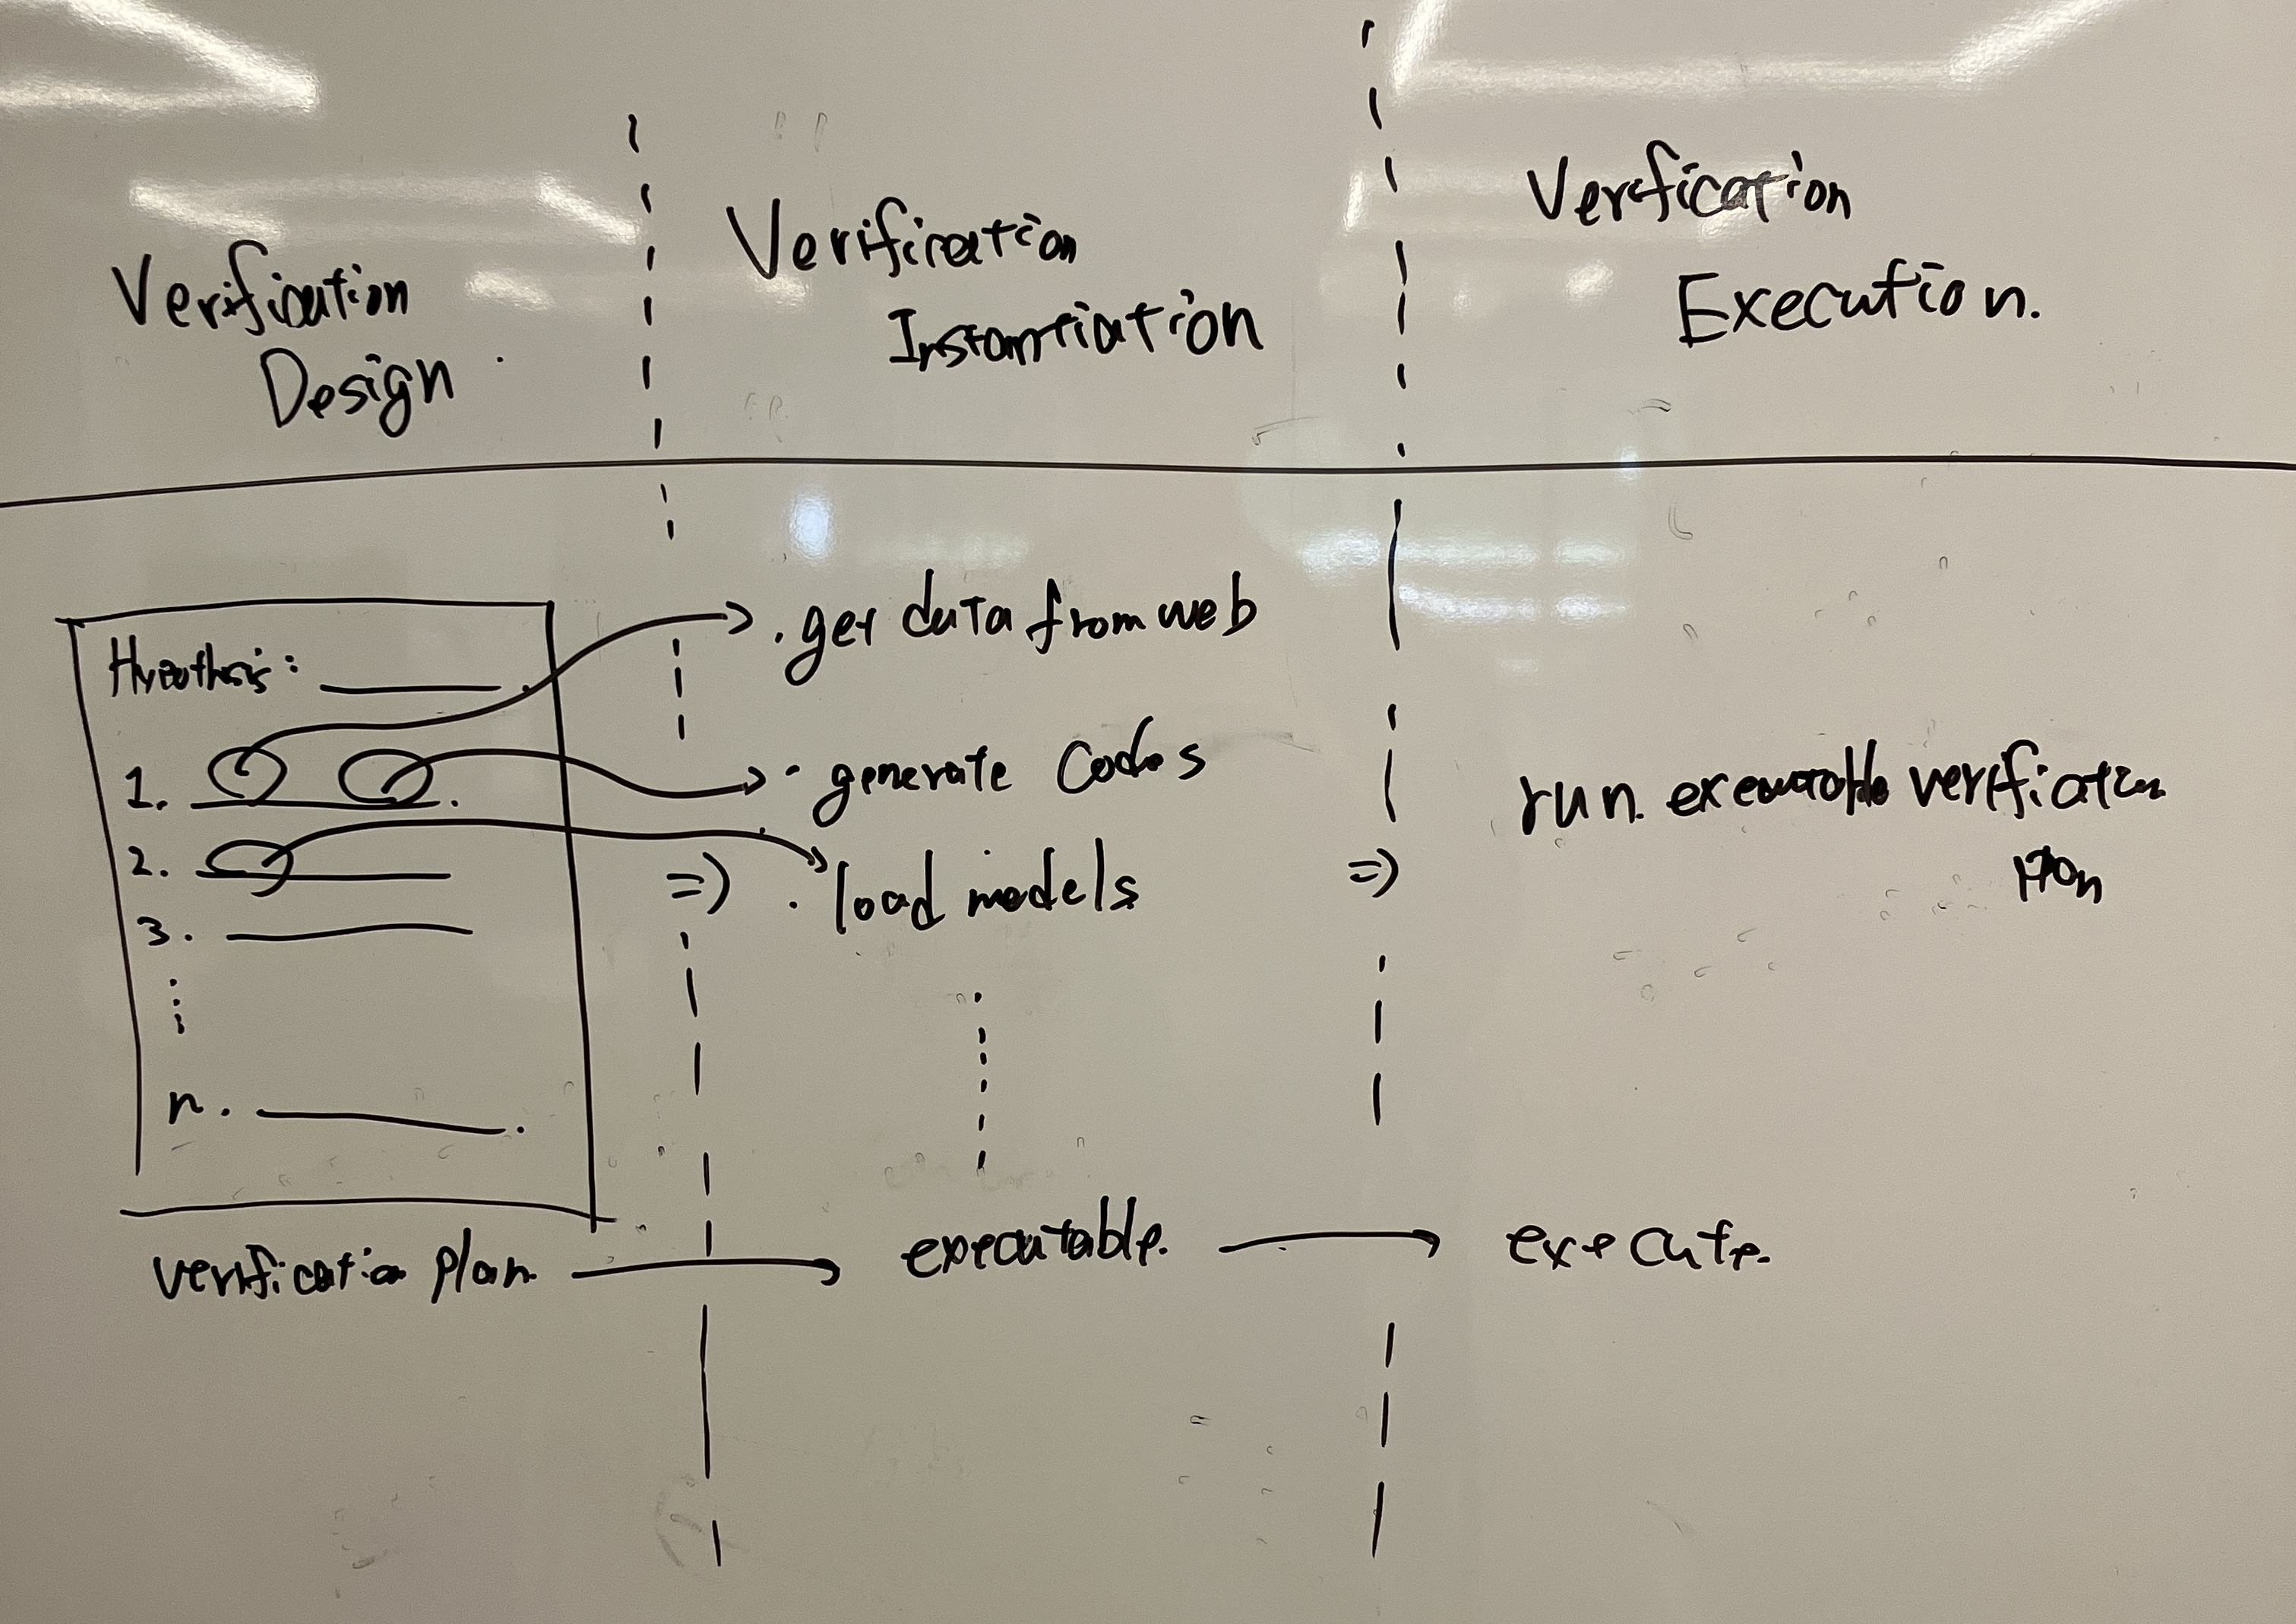
\includegraphics[width=\textwidth]{figs/verification.jpg}
    \caption{Verification}
    \label{fig:verification}
\end{figure}

\subsubsection{Verification Design} 
In verification design, the agent will create a plan to execute the verification, which consists of hypotheses, verification criteria (criteria to determine if the output confirms or refutes the hypotheses), and the procedures for conducting the verification. The verification plan should be specific and detailed enough so that anyone faithfully executing it can reproduce the same verification process and result. For example, suppose I am considering an experiment to compare a proposed method with a baseline and validate the hypothesis that the proposed method performs better. In this case, the plan should describe in detail which model to use, what dataset to employ, and how to measure the performance. Thanks to this specification, I can separates the two functionally distinct stages of verification: the phase of considering what needs to be validated and the phase of actually executing the verification.

It is during the verification design stage that specific skills for hypothesis verification are required. This is because automating the preparation and execution of a plan involves the automation of more general intellectual tasks, not limited to research automation, while creating a verification plan demands an explicit understanding of what verification entails and what criteria constitute a successful verification. In aiming to automate this verification plan, the key lies in teaching machines how to understand the concept of verification.\footnote{
Even humans may sometimes do verification without proper understanding of the method. For example, someone may conduct hypothesis testing just because ``everyone does it.'' While this may be an extreme example, it is not common for researchers to understand the epistemological implications of inductive reasoning and statistical inference and in what sense I can say I verify a hypothesis. In that sense, the requirement for machines to understand verification may be somewhat challenging. However, if the aim is to truly enable AI to autonomously conduct research, it appears crucial for the AI to have a proper understanding of what constitutes verification.
}

% Multiple abilities are needed to create a verification plan, but based on the discussion so far, it is evident that at least two abilities are required.


% At this stage, I contemplate how to validate the hypotheses and proceed to formulate a verification plan. In a verification plan, the agent writes about the hypotheses, verification criteria (what will be considered as evidence for verification), and the procedures for conducting the verification. These plans should be as much detailed as possible. The Fig. provides an example in the context of machine learning. The idea is to create a blueprint for a pipeline where verification is automatically executed by faithfully following the plan.

% Furthermore, for artificial intelligence to perform autonomous verification, it seems essential that the AI not only adopts certain verification criteria but also be able to explain the meaning behind them and how they contribute to the verification process. Even humans may sometimes engage in this without conscious awareness, such as conducting hypothesis testing because ``everyone does it.'' In that sense, this requirement may be somewhat challenging. However, if the aim is to truly enable AI to autonomously conduct research, it appears crucial for the AI to have a proper understanding of what constitutes verification and be able to design it itself or, at the very least, explain it adequately.

There are several abilities that a machine must possess in the context of verification planning, but based on the discussion so far, it is evident that at least two abilities are required: understanding what verification is and planning to achieve objectives.

Let's first discuss the ability to understand verification. As mentioned in the sections on question construction and hypothesis generation, this is an extremely crucial ability in the overall automation of the research process. As before, the extent to which ``understanding'' is required depends on how much autonomy is expected in the automation of verification. If that is used as a verification tool for humans, what machines to do is just using human verification methods properly. On the other hand, if they were required to understand the concept of verification from scratch, I would face a lot of challenges as I just described in this chapter. 

If you aim to achieve the former, one of the initial steps could be creating a dataset specifically tailored for verification. By gathering research papers that utilize widely used verification methods like statistical hypothesis testing, you can train a model to construct verification methods from these hypotheses. One naive approach could be to start by generating method descriptions in research papers from the given hypotheses. 

If you were to achieve the latter, you might want to begin by contemplating what beliefs mean for machines. Alternatively, placing agents in situations where verification becomes necessary could implicitly help them acquire the concept of verification. In this case, addressing the issue of generalization across environments, such as enabling machines to explicitly reuse the concept of verification, will be crucial. Eventually, as repeatedly emphasized, discussing how to resolve the alignment problem will be necessary.

% If artificial intelligence is used as a tool for human research, it is sufficient for artificial intelligence to faithfully reproduce what humans do as verification. For example, it would be great if it could use basic concepts such as hypothesis testing, controlled experiments, and interventions and automatically create experimental plans based on them. In this case, it is not necessary for the machine to strictly know why it constitutes verification, as long as it can learn from numerous examples of human verification and use it appropriately. In other words, in this case, the required understanding can be described as indirect and practical understanding through examples of human usage. Furthermore, if it can understand the concepts of hypothesis testing and controlled experiments from first principles, it would be a significant achievement in terms of automatic verification.

% On the other hand, if artificial intelligence itself is allowed to conduct research for its own knowledge generation, it seems that artificial intelligence needs to understand what verification is, whether explicitly or implicitly. And similar to the unknown nature of the answer to a problem, it seems to be an ability that cannot be acquired just by observing examples of human verification. This is because verification involves updating the beliefs of the members of a society, which depends on the nature of the beliefs of the machine group itself. Whether the knowledge generated by such agents is understandable by humans or can say something about nature is not obvious, but this will be discussed in detail in later chapters.

Let us move on the second ability: planning. Understanding verification is a necessary condition for setting verification criteria by considering what can be tested against a given hypothesis. When conducting actual verification, under the assumption of a hypothesis and verification criteria, one must devise procedures for carrying out the verification. For example, in experimental research, let's say a hypothesis A is formulated, and a verification criterion is established that considers the hypothesis valid if it meets certain criteria through statistical hypothesis testing. To actually perform this verification, it is necessary to generate data to be used for verification, and if there is no apparatus to generate the data, one may need to create it. Thus, in a verification plan, one must develop a plan to fulfill the purpose of executing the verification.

Creating a plan is known to be a challenging task, not limited to verification plans. To achieve a goal, one must understand what is necessary and comprehend the appropriate sequence of steps to achieve the goal. As mentioned earlier in the section on constructing questions, when creating a plan, it is essential to consider feasibility, taking into account the complex external factors such as current financial capabilities and accessible resources. Understanding and incorporating these constraints appropriately can be a highly challenging task, as they are intricately linked to various external factors.

While there are already a difficult task, the particular challenge in creating verification plans for research lies in the fact that one may need to create things necessary for verification if they do not already exist. This is an extremely high-level difficulty problem. To carry this out, one must first accurately identify what is currently lacking. After recognizing the deficiencies, one must consider how to create what does not exist. Once the method is known, materials for creating it must be prepared, and it must be actually built. And even if it is created, one must investigate whether they function properly. This is an unbelievably complex task, and it seems highly unlikely to simultaneously expect the creation of such intermediate products by directly generating a verification plan from the verification itself. Therefore, in aiming for true automation of verification, it is crucial to seriously consider how to solve this problem.


Finally, once the necessary elements for verification are understood, they need to be represented as something that can be understood by other researchers. This is not a requirement of a verification plan but a necessary condition for knowledge to become knowledge for society. In order to generate knowledge for society, it is necessary not only to verify hypotheses but also for the verification procedures to be understandable to other members of society and judged as valid.\footnote{
While it is desirable for the question generation process and hypothesis generation process to be publicly available, it is of utmost importance that the verification process is disclosed. 
} Also, as discussed in the section on hypothesis generation, verification must ensure that the causes behind the verification results are traceable as much as possible. While this is not an inherent requirement of the act of verification a hypothesis, it is a crucial characteristic needed for proper interpretation of verification results and for better knowledge production through hypothesis testing. As mentioned earlier, it is impossible to enumerate all potential assumptions, so it becomes necessary to explicitly state assumptions as comprehensively and in as much detail as possible to make the process realistic. Recognizing the underlying assumptions, including those behind the scenes, and selecting which assumptions to prioritize as potential causes of the results, is indeed a challenging task.



\subsubsection{Verification Instantiation} 
At this stage, the research plan that has been developed is translated into an executable instance. For example, if the research plan states, ``Train the model B with the dataset A...'' the necessary steps would involve acquiring dataset A from the appropriate source, formatting it to be compatible with the model's input requirements, and preparing the data for training, etc. Similarly, if the plan states, ``When a rat presses the switch B, food is dispensed...'' the agent has to prepare rats, food, and create a machine that dispenses food upon pressing the switch, and so on. This process involves translating the plan into physical or computational instance for execution.

\begin{figure}[htb]
    \centering
    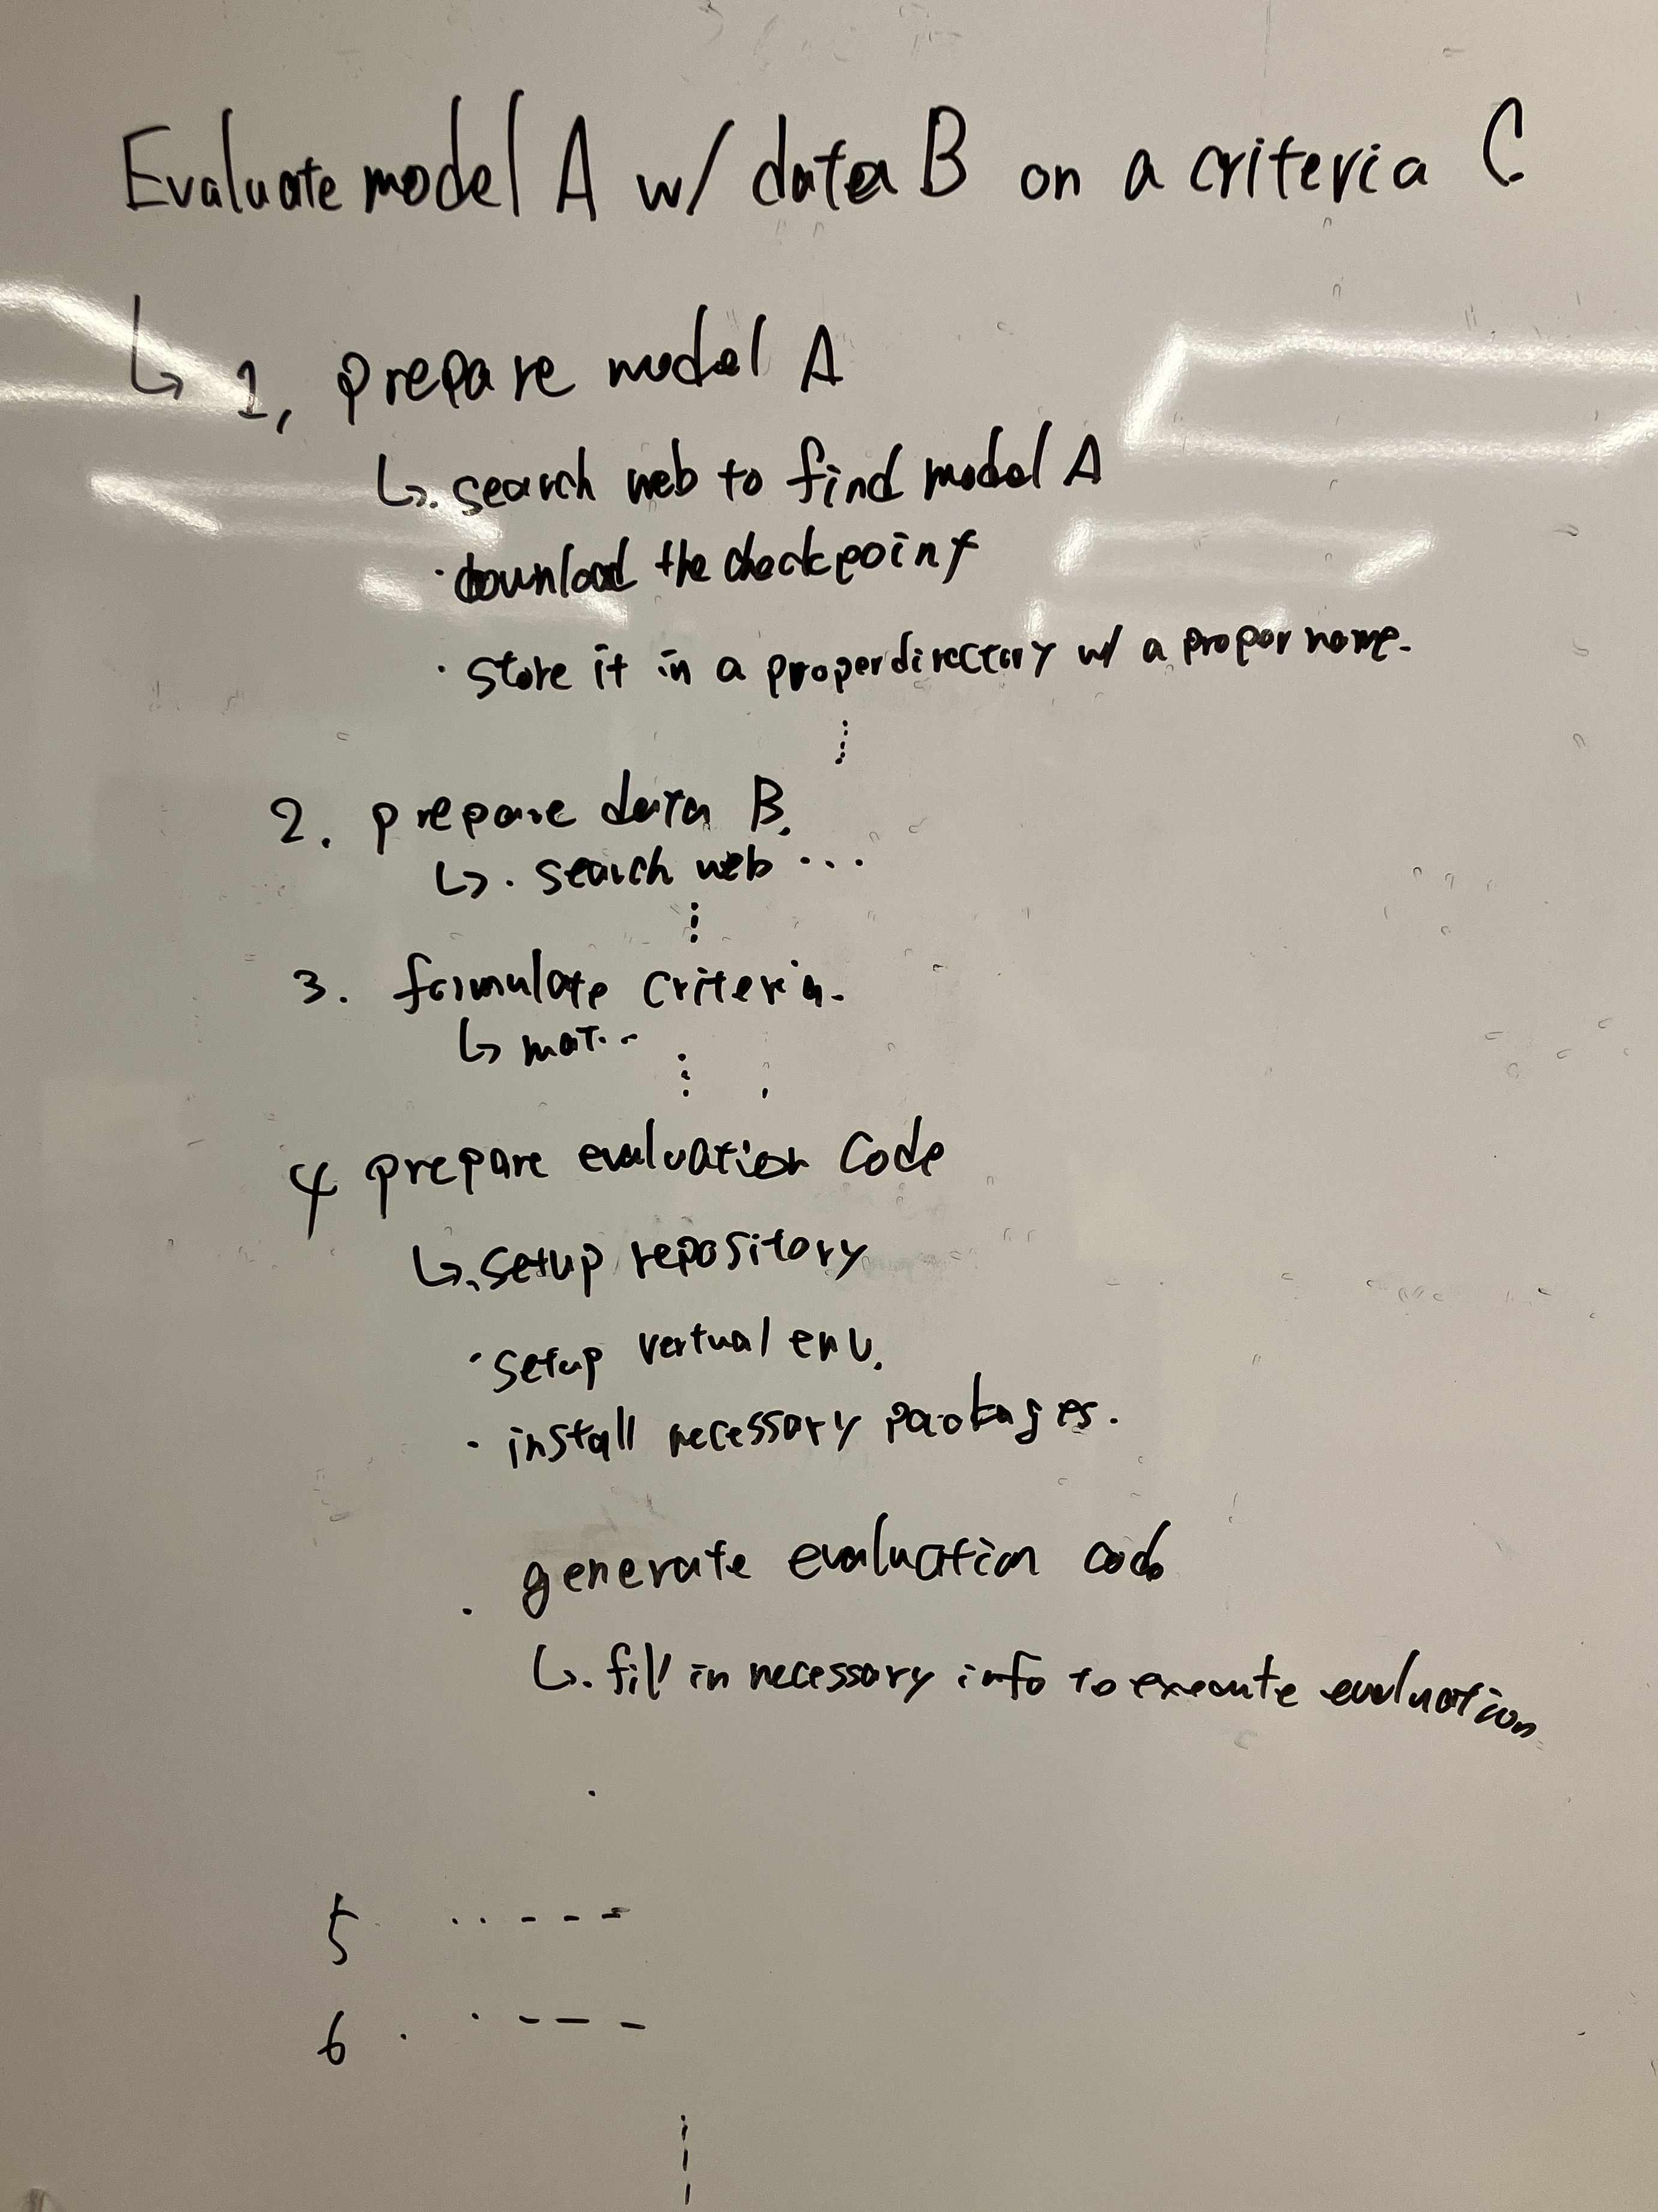
\includegraphics[width=0.5\textwidth]{figs/verification_instantiation.jpg}
    \caption{Verification Instantiation}
    \label{fig:verification_instantiation}
\end{figure}

As evident upon reading, this process is highly challenging to automate. Even research confined to the realm of computers, such as research of computer science, requires accomplishing a vast number of complex tasks. For research that necessitates physical realization in the real world, the development of robotics and embodied agents are necessary. Regarding the question of where and how to tackle these problems, I will provide my perspective in the later chapter. However, it is important to note that unless the research is constrained by questions and hypotheses, aiming for true automation will inevitably require overcoming these challenges

To reiterate, this process can be accomplished through the automation of actions, and it does not necessarily require unique technological developments for research automation. For instance, in studies that are entirely computer-based, automating all actions within the computer system would suffice. In recent times, attempts have been made to have language models operate computers, and the progress in such research corresponds to the advancement of automation in this process. If the research involves activities in the physical world, achieving full automation of human movements (or their equivalents) would make this process feasible. Therefore, research focused on developing humanoid robots that can move like humans will contribute to the automation of this process.

% Once a hypothesis has been established, a verification plan is created to determine how to verify it. The specific method of verification depends on the subject being investigated, making this aspect of research difficult to structurize and automate in a unified way.

% However, in many empirical sciences, the likelihood of a hypothesis is evaluated based on statistical significance. This is done by \textit{hypothesis testing} in practice. As this is a hypothesis test, it can only reject the null hypothesis, rather than directly determining the correctness of the hypothesis. Therefore, it can only be said that the hypothesis has survived for the time being. The belief that the surviving hypothesis is more likely to be valid is the basis for decision-making.

% In any case, humans seem to use statistics or probability as the basis for assessing the validity of a hypothesis. In other words, I seem to concede to consider a hypothesis as plausible if something that cannot happen by chance, such as observing the same number repeatedly. This is based on the assumption of the ``principle of confirmation,`` which assumes that if the number of observations increases, it can be considered more reliable, and the ``principle of uniformity,`` which assumes that things will continue to proceed as they have been if the conditions remain the saus. These beliefs ultimately serve as the basis for verification and scientific knowledge production. 

% I will not delve into the validity of these beliefs here. What matters is that my research activity follow a practice that ``when a hypothesis is present, and a certain criterion and procedure are prepared, and the hypothesis is considered valid according to that procedure, I consider it valid.''

% In theoretical research, sometimes there is no verification plan. Theory is a hypothesis, and its validity is determined separately through verification (not in the sense of whether it is mathematically valid, but for example whether it explains physical phenomena or not). However, in complex modern science, theorists propose a theory, and experimentalists verify it.

% Therefore, it is understood that in current research practice, shared knowledge in the form of papers may not necessarily provide a complete answer to a given question. This is similar to research on negative data. Negative data cannot solve the unknown initially declared, but it can reduce a certain degree of uncertainty towards it. This is because the validity of the presented hypothesis may have decreased somewhat. If this is the case, each research shared in the form of a paper may be more appropriate to describe as "reducing uncertainty towards the unknown," rather than "making the unknown known." This can become complicated when scrutinized strictly, so let's put this aside for now and continue to discuss how "producing new knowledge" is research.

% In reality, conducting research is expected to be done with limited resources (time, funding, computing resources, people, etc.). Therefore, it is necessary to consider these resources when determining the verification approach. After a research design is determined at an abstract level, the feasibility of the research plan is roughly evaluated through a simple problem setting. This is known as a pilot study.



\subsubsection{Verification Execution}
Finally, the instantiated research plan is executed according to the prescribed procedures. In verification design, I am crafting the essence of the verification, and during verification instantiation, I am preparing it to be executed in a concrete and feasible manner. Therefore, there are almost no tasks to be done in this process. The preparation for verification, being distinct from the actual execution of verification, is not a verification in itself. With this understanding, I have adopted this formal classification for the current context.
\footnote{
Typically,``experiments'' refers to the data generation process and subsequent analysis and interpretation are conducted separately. However, since I am discussing a verification plan in this context, all of them are in the same single plan. Therefore, please note that what emerges from executing the verification plan is not data but the verification results.

In many empirical studies, the data generated from experiments is often used not only for the verification of hypotheses but also for generating new hypotheses or giving some insights. However, as hypothesis generation and hypothesis verification play different roles in knowledge production, I do not assume any uses of the generated data beyond verification in this context. Of course, please note that this does not imply that such actions are prohibited in practice. Data analysis will be discussed in a separate section.
}

\subsubsection{Starting from Verification Design}

As mentioned above, I believe that the verification process can be divided into three stages: formulating a verification plan, preparing for the execution of the verification plan, and executing the verification plan. Among these stages, the execution of the verification plan and the preparation for it require interaction with the physical world in many fields. For example, in certain fields, you may need to purchase and raise rats for training, while in others, you may need to observe physical objects directly. On the other hand, formulating a verification plan is a process that is purely confined to the human mind in a wide range of fields. Therefore, it can be a good idea starting from automating verification design process.

% As mentioned earlier, in the case of empirical sciences, testing is often performed. Therefore, data is first generated, processed, and finally verified using the processed data. If I summarize the process of generating and processing raw data as data generation, this process can be broadly divided into data generation and judgment based on verification criteria. It may be rather said that the act of research itself is a process of repeatedly generating data and performing some kind of processing on it.

% I separated the verification plan from the verification because I want to separate the description and execution of the process. The verification plan is analogous to coding, while the verification is more similar to executing the code.

% The output of this process is usually wrtitten in the result section in the paper.

% \section{Conclusion}
% In this chapter, I discussed what research is. Research is the act of producing new knowledge for a community of constituents capable of forming shared beliefs. I characterized the production of new knowledge as the process of posing unanswered questions, generating hypotheses in response to those questions, and verifying them. Additionally, starting from the standpoint that knowledge is belief, I also presented the depiction of research as belief updating.
% \textcolor{red}{TODO}


% \chapter{Challenges and Ideas}
% In Chapter 2, we examined the definition of research and its implications, and in Chapter 3, we provided an overview of past efforts related to the automation of research. In this chapter, based on these, we will reorganize the challenges towards realizing an autonomous and general artificial intelligence capable of conducting research.



\section{Challenges}

 \subsection{General and Autonomous Question Construction, Hypothesis Generation, and Hypothesis Verification}

 In Chapter 2, we explained that in order to create an AI capable of conducting any research, it is deemed necessary to realize the formulation of questions, generation of hypotheses, and validation of these hypotheses as a combination of universal skills applicable to all research. In this section, we will revisit and organize the potential challenges in achieving an AI that can conduct each of these processes.

 \subsubsection{Common Challenges}
One of the major challenges that can be a common issue for any process, as pointed out in prior research \cite{coley2020autonomousII}, is how to execute these tasks in open-ended situations. For instance, in the automation of experiments, robots use experimental equipment selected, prepared, and set up by humans. However, humans do these tasks from scratch with their own hands. Humans do not use a given corpus of papers; instead, they search for and use them on their own. Candidates for hypotheses are not explicitly provided; humans begin by identifying potential hypotheses. Even when formulating questions that serve a particular goal, humans set that goal themselves. 

In many cases in research automation, these elements are pre-determined by humans. How to let machines autonomously perform these tasks starting only with the same initial information given to humans is crucial in realizing an autonomous artificial researcher. Moreover, having this kind of freedom is essential to achieving a general artificial researcher as well. This is because if we impose constraints on AI to research only within specific research questions or hypothesis spaces defined by humans, it cannot become an AI capable of conducting arbitrary research. Therefore, a significant challenge is how to make AI acquire complex foundational skills and fundamental reasoning abilities to realize these capacities.

\subsubsection{Question Construction}

The first issue discussed in Chapter 2 is the problem of determining the unknown nature of the answer to a question. Given that research is an endeavor to produce new knowledge, it is necessary for the answer to the question to be unknown. Therefore, there is a need to generate such questions or later verify that the answer to the question is indeed unknown.

The second challenge is the issue of how to make a machine generate a ``good'' question. Firstly, what researchers consider as a ``good'' question is not always consistently agreed upon among them. Furthermore, we pointed out that the ``goodness'' of a question is inherently a concept relative to the individual or society. Hence, there seems to be a need to clearly define what constitutes a good question and think about how to effectively integrate these definitions.

The third challenge is that as we demand more autonomy from AI, the automation of question formulation becomes more difficult. Inherently, questions are constructed based on various motivations, such as pure intellectual curiosity or for specific objectives. It is very challenging to automate the construction of questions without defining which of these motivations should be the source. Moreover, as mentioned in Chapter 2, the construction of questions encounters the problem of infinite regression when pursued with strict autonomy. Even if not taken to that extreme, setting higher-order objectives behind questions for AI is an exceptionally difficult task.

It seems that the automation of question formulation has received relatively less attention compared to other processes. Since the formulation of questions is an essential element in conducting research, it would be desirable for more focus to be directed towards the research on automating this process.z

% Realizing AI that construct a ``good'' question in a generic way is challenging. As discussed in Section \ref{section:the-relativity-of-knowledge-production-to-society}, research is relative to society and different criteria can be considered for what makes a ``good'' question. Thus, some human perspective on the ``goodness'' of a question must be incorporated. We need to discuss what we consider good, what we should prioritize, and how to incorporate the value to AI.

% \textcolor{red}{TODO}

% Moreover, determining inputs to the question construction module is not trivial. In hypothesis generation, the question is the primary input, whereas in verification, it's the hypothesis. However, question formation take any input. Once you seriously try to identify the origin of question, you will encounter infinite regress. This is a unique problem that arises when aiming for a general-purpose and autonomous artificial researcher. This is because the issue revolves around how much input can be assumed while still being considered autonomous, given that it can potentially take any input.

% \cite{wang2023skillqg}

% neural question generation \cite{pan2019recent}


\subsubsection{Hypothesis Generation}

One challenge in creating an intelligence capable of hypothesis generation, not just as a tool for humans, is the need to empower the machine itself to form plausible hypotheses for questions to which even the machine doesn't know the answer. Current machine learning models have been criticized for potentially not knowing what they don't know \footnote{
In our discussion with Wataru Kumagai, we were reminded once again of the importance of self-awareness in creating an AI capable of conducting research.
}. 
Moreover, they are known to confidently provide answers or fabricate falsehoods about topics they are ignorant of. Therefore, it seems essential to first accurately recognize what is unknown, either for oneself or the world at large, as told in sections of question construction. Upon facing an unknown subject, there's a need to reduce uncertainty and approach understanding. As mentioned in Chapter 2, humans attempt to understand uncertain subjects by gathering information from papers, experiments, or by reframing questions. While it may not be necessary to adopt the exact same approach, it seems essential to enable machines to autonomously adopt strategies to reduce uncertainties.

% Outputs from machine learning models are essentially inferences tinged with uncertainty. From this perspective, one could posit that these models are already inherently generating hypotheses. Indeed, they are already employed for hypothesis generation in numerous scientific investigations.

% However, while these hypotheses might be hypotheses in the sense that the answers are unknown to humans, they might be self-evident to the machine learning model. When we talk about AI generating hypotheses in the context of AI conducting research, the ultimate expectation is for the AI to provide plausible answers to what is unknown to AI itself. This remains an unresolved issue.

As one of the promising approaches for tacking unknowns, it seems crucial for AI to acquire systematic thinking to realize this, as humans developed systems like language and mathematics, allowing them to infer about subjects beyond their experience. Systematic thinking is not only important for out-of-distribution generalization but is also valued for interpretability, causal inference, logical reasoning, mathematical processing, and planning.

\textcolor{red}{TODO}

\subsubsection{Hypothesis Verification}

In Chapter 2, we highlighted several challenges in realizing an AI capable of verification. First and foremost, the AI itself needs to understand what verification is, and by what criteria a sequence of actions qualifies as verification. Ideally, it would be preferable for the AI to contemplate and understand from scratch what verification is. However, many humans don't do this either, and as discussed in Chapter 2, the philosophical debate on precisely defining verification is still unresolved. Therefore, it's harsh to demand this of a machine. At the very least, the machine needs to thoroughly understand and proficiently use verification concepts that humans employ, such as statistical hypothesis testing, from first principles.


Second, the AI must be able to formulate detailed and complex plans to verify a hypothesis. With the advancements in language models in recent years, we are now much more capable of formulating superior plans than before. However, devising detailed plans remains a challenging issue.

Third, it has to be prepared to carry out these plans and execute the plan with the combination of human-like complex actions.As mentioned in Chapter 2, to achieve this, the AI must be able to search for, create, purchase, and manipulate equipment with almost the same degree of freedom as humans, requiring it to exhibit extremely sophisticated and complex behaviors. This is an immensely challenging issue, and it might even be fair to say it's one of the biggest bottlenecks in realizing an intelligence capable of generic and autonomous research. Laboratory automation have attempted to address this challenge in real world by developing robots. We will discuss the case within the computer below.

For AI to execute research on a computer, it must perform any operation within the computer. For instance, machine learning research entails, setting an environment, preparing datasets and models, and writing and executing codes. To allow AI to prepare these without human intervention, the AI itself must be able to autonomously search the web, select data, download it, and so on. Furthermore, once the AI generates code for verification, it must operate the shell to execute it.

There are ongoing initiatives to enable language models to operate browsers \cite{nakano2021webgpt,act1}. While full browser operations might seem ambitious, there are already endeavors to allow language models to conduct searches \cite{mialon2023augmented}. If we achieve browser automation, it will greatly advance research automation involving web operations. Moreover, efforts like the open interpreter \cite{openinterpreter} aim to automate any computer action. This direction holds promise for automating all research confined within a computer. Although these studies are gaining traction in the machine learning domain, they're not always linked to research automation. We advocate recognizing this as a pivotal challenge in the realm of research automation.

In the field of machine learning, it seems that the discussion on automated validation has not garnered much attention until now. However, recently, the need for verification is recognized in the machine learning community beyond outside of the context of research automation. Studies like \textit{scientific claim verification}, which received much attention during the COVID-20 pandemic \cite{wadden2020fact}, or attempts to minimize hallucination \cite{dhuliawala2023chain} are examples of them. These are not attempts to automate validation in research. Therefore, these findings cannot be directly applied to the automation of research validation. However, we expect that these studies will provide useful insights for the future development of artificial intelligence capable of understanding validation.

% Creating AI that autonomously verifies hypotheses is challenging. While current models can mimic human verification, truly understanding the verification strategy demands more work. Sometimes, they even need to devise the verification measure themselves.

% The biggest challenge for autonomous verification is the need to freely move around in the real world or within a computer, and to manipulate objects within that world at will. We believe this to be one of the greatest barriers to full research automation. Laboratory automation have attempted to address this challenge in real world by developing robots. We will discuss the case within the computer in Section \ref{section:behaviour-inside-the-computer}.

% \subsubsection{AI Capable of Peer Review}

% Given the difficulty of these challenges, automating peer review could be a strategic starting point. This is because peer review is a universal process across diverse research fields and it assesses the validity and quality of problems, hypotheses, and verification methods, which is easier than generating them. Despite some progress, full automation is still elusive \cite{yuan2022can,schulz2022future}.


% \subsection{Behaviour inside the Computer}
% \label{section:behaviour-inside-the-computer}


% Lab Notebook?
% \subsection{Dataset of Research Process}
% It is important to establish the necessary infrastructure for research automation. The two pillars of research automation are the development of basic models that incorporate academic knowledge and the construction of data sets. The development of an infrastructure model that incorporates scientific knowledge has already been proposed in many places and is actually under development, so I will not emphasize its necessity here again. Also, regarding data sets, the construction of data sets for the acquisition of scientific knowledge has been done in various places as well, so I will not emphasize that here either.

% Instead, we propose here to construct a research process dataset. A research process dataset is behavioral log data that incorporates all possible tasks throughout the entire process of the study, from start to finish. Ideally, individual tasks should be labeled as to whether they correspond to question construction, hypothesis generation, or hypothesis testing. We believe that building such a data set is important because, as explained in the Literacy section of Chapter 2, the current paper is not a data log of the entire research process. This makes it difficult to be data-driven and end-to-end learning how to do research itself. I believe that building a research process will help solve these problems and increase the likelihood of more flexible intelligent agents.

% However, building a dataset of the research process seems daunting. This is because researchers who do not currently keep research logs would have to go to the trouble of recording their research process.\footnote{
% In an experimental laboratory in the natural sciences, it is common to take research notes, so it may not be that difficult to record more detailed processes as an extension of this practice. However, in the machine learning field, the culture of taking research notes does not seem to be that common. (We think it is common to keep logs of experiments, but it seems to be rare to describe the details, for example, where and how the data was obtained.) 
% } Therefore, it seems necessary to devise a way to make it easier for researchers to keep logs. It may be to manage the research process on GitHub, or to take research notes as in natural science research, but it is important to discuss how to achieve these things.

% Being able to construct a dataset of the research process would be ideal, but may not be immediately feasible. As an alternative, it seems important to create a dataset designed to automate question construction, hypothesis generation, and hypothesis testing. At its simplest, one might start by building a dataset of papers labeled with the parts that correspond to the question, hypothesis, and test, respectively. This would be a relatively simple but important step in achieving a generic artificial researcher.

% Alternatively, instruction tuning could be done by viewing question construction, hypothesis generation, and hypothesis testing as tasks, respectively. This would produce a language model that can execute question construction, hypothesis generation, and hypothesis testing with greater fidelity. This could be the foundation for a general-purpose, autonomous artificial researcher.



\subsection{Alignment}
As discussed in Section 2, when realizing an AI that autonomously conducts research, the issue of alignment arises. 

First and foremost, it is essential to consider ways to ensure that AI does not engage in research that could harm humans. However, this is a challenging issue. The problem of ensuring that AI does not harm humans is a difficult problem in AI Alignment. Furthermore, knowledge and technology produced by research are fundamentally value-neutral. That is, the knowledge can be used for good or ill. Therefore, even if AI were to research with harmful intentions, it would be challenging to judge from the actual research results.

The remaining two issues arise in the ultra-long term when AI becomes fully autonomous in conducting research. The second issue is that to enable meaningful knowledge production for humans, there needs to be an alignment between the knowledge systems of AI and humans. As mentioned in Chapter 2, if knowledge and verification are relative concepts to society, research conducted autonomously by AI may become meaningless to humans. On the other hand, if we were to correct AI to follow human methods entirely, we might unnecessarily limit the machine's potential capabilities. Deciding how much human methodology and values to incorporate and how much freedom to allow the machine, and finding ways to achieve this, will be a significant challenge in creating research-capable AI.

The third issue concerns the alignment between AI and nature, not between humans and AI. As mentioned in Chapter 2, the fact that humans have come to understand nature is likely not unrelated to our long history of interacting with nature. It seems there's no guarantee that artificial machines like AI, which lack such experiences, would lead to an understanding of nature through their autonomously generated knowledge.

The latter two issues are problems that only arise when demanding extreme autonomy from machines and are not immediately problematic. However, when discussing the limitations and possibilities of knowledge production and natural understanding by agents independent of humans, they seem to become relevant issues.

% In the medium to long term, it's essential to devise ways to ensure that AI doesn't engage in research that could be dangerous to humans. 

% In the long term, we must contemplate how to construct a knowledge system that are mutually translatable between human society and AI society. While these issues may not arise in the short term, it's crucial to engage in discussions now, looking towards the long-term future.

% \subsubsection{Understanding}

% Extensive discourse transpires concerning scientific discoveries. Yet, discussions pertaining to scientific comprehension remain relatively unexplored. Krenn et al. delve into the conundrum of what it entails for a machine learning agent to not only unearth scientific knowledge but also to comprehend it \cite{krenn2022scientific}. They adopt a human-centric stance, positing that an agent's ability to offer explanations comprehensible to human scientists signifies the existence of its scientific understanding.

sun-rise \cite{leslie2023does}

\section{Ideas for Elucidating Challenges}

\subsection{Prototyping General and Autonomous Artificial Researcher}

Realizing a general and autonomous AI capable of research is an exceptionally challenging issue that will likely take a long time. The challenges mentioned in the previous section are just the tip of the iceberg, and there are undoubtedly many more yet to be identified. Therefore, it seems crucial to start by identifying and addressing unknown challenges to reduce uncertainties. A good starting point might be to develop a prototype of a general and autonomous AI capable of research.

Let's discuss what this prototype might entail. As reiterated earlier, research, we believe, consists of constructing questions, generating hypotheses, and verifying these hypotheses. Thus, it seems appropriate for this prototype to consist of three main modules: question construction, hypothesis generation, and hypothesis verification. The question construction module takes any input and produces a question. The hypothesis generation module takes this question as input and produces a hypothesis. The hypothesis verification module takes the hypothesis as input and provides verification results.

For the prototype to be autonomous, human design, implementation, and intervention should be minimized. Consequently, each module, aside from receiving minimal inputs, should autonomously gather information from the world humans typically interact with. For instance, aside from the question input from the question construction module, the hypothesis generation module shouldn't have predetermined inputs. This module could have touchpoints with the physical world or the digital realm, acquiring necessary information and generating hypotheses as humans do.

Furthermore, for the system to be general, the internal workings of each module mustn't depend too much on specific research topics. For example, if the verification method is an algorithm planning and executing experiments for a specific physics research, it can't be used for psychological research. Also, if the verification method is an algorithm to plan and conduct experiments, it can't be used for deductive research. The inner workings of the hypothesis verification module should be as minimal as possible, limited to only what is necessary for hypothesis verification. 

This is akin to an abstract class of research. Creating a system that meets both autonomy and generality requirements while properly constructing questions, generating hypotheses, and verifying them only with this abstract system is too challenging, even in simpler scenarios. Hence, it might be necessary to impose some constraints on this abstract framework initially. Discussing the extent of these constraints, why they're needed, and how they can be eliminated will help elucidate the challenges in realizing a general and  autonomous AI researcher. By identifying these challenges and turning them into research themes, and then advancing foundational research, we believe we can more efficiently approach the goal. In the following, we will list up such potential constraints to provide a first step.

\subsubsection{Candidate Constraints in Prototyping}

% \subsubsection{Grand Goal is Given}
As we've emphasized repeatedly, constructing questions from open-ended situations is a challenging task where even a starting point for resolution is not visible. Therefore, it seems prudent to start by determining in advance what the input for constructing the question should be, separate from the unrestricted information sources that the module can access. For such input, it might be appropriate to consider the overarching goal we ultimately want to achieve as the minimal input. As stated in Chapter 2, not all research questions are necessarily constructed to achieve some grand goal. However, many studies build their questions by breaking down such objectives. Consequently, if research can be conducted to construct questions from overarching goals, then a vast majority of human-conducted research, and notably ``meaningful'' research, potentially becomes feasible.

% \subsubsection{Research is Completed Entirely within a Computer}
One of the biggest bottlenecks in realizing a fully general and autonomous artificial researcher is the necessity for complex actions in the preparation and execution of verification. Especially, developing a robot capable of acting freely in the physical world like humans is an extremely challenging task, and it carried difficulties beyond just AI research. Therefore, it seems reasonable to first consider research that is confined within a computer for prototyping purposes. Specifically, it means envisioning a world where AI can interact not in the physical realm but within the computer environment. Some computer science research falls under this category. Of course, realizing an AI that can freely operate within a computer is also a very challenging issue, but it seems more feasible than an agent freely operating in the physical world. The purpose of prototyping is to materialize the concept, even if it's rudimentary, and identify challenges. Therefore, it seems desirable for prototyping to first limit the target environment to within a computer and wait for the advancement of foundational research for the realization of free activity in the physical world.

% \subsubsection{Verification is Limited to Humans'}
The issue that allowing machines to conduct research entirely autonomously could result in constructing knowledge systems meaningless to humans arises when we try to let AI construct even verification from scratch. This is necessary if we want to truly say an AI can verify on its own. On the other hand, many people probably have no interest in generating knowledge that is meaningless to humanity. In the first place, even if such a thing were realized, humans might not be able to evaluate whether the AI has truly constructed a meaningful knowledge system for them. Also, I don't think human researchers always understand or construct verification from first principles. Therefore, it might seem harsh to demand these of AI. So, it seems preferable to first ensure that AI understands and can always use the verification methods that humans use. Specifically, we aim to make sure AI can always proficiently use experiments, statistical hypothesis testing, proofs, etc. By doing so, I believe there's a possibility to realize an AI that conducts highly generalized, autonomous research that is meaningful to humans.

\subsubsection{AI that Conducts Machine Learning Research}
Providing a grand goal or limiting the action space can restrict the targeted research field. We believe it might be beneficial to aim for the realization of AI that can conduct machine learning research as prototyping. Firstly, some machine learning research can be fully completed on a computer, meeting the aforementioned constraints. Furthermore, machine learning technology is essential for the realization of research-capable AI and currently serves as a foundational technology in many research fields. Thus, if machine learning research can be fully automated, it will not only advance the study of automating other research areas but also accelerate the automation across many disciplines. This suggests that starting with the automation of machine learning research might be a good approach to speed up the development of research-capable AI. Moreover, in machine learning, there are already efforts underway, such as AutoML and MLOps, to automate parts of the machine learning research workflow. These achievements will likely further assist in creating AI that can conduct machine learning research.

\subsubsection{Implementing Each Module with Large Language Models}

Considering the remarkable performance of recent language models and the necessity for general-purpose research, it seems reasonable to first represent each module as a large-scale language model. While there are increasing efforts to construct pipelines by connecting large-scale language models, we will prototype the overall research execution system by connecting language models in a similar manner. To ensure this system is open-ended and general-purpose, prompts given to these language models will consist only of general instructions that can be applied to many types of research. For instance, an instruction like "generate a hypothesis for the following question" is a command that can be given to a hypothesis-generating module in not just machine learning research but any field of research. Naturally, merely providing such instructions won't yield perfect results from the get-go, so there may initially be a need to provide additional auxiliary directions. However, even these instructions will be kept as general as possible.

For open-ended operations within a computer space, ideally, the system should only be given access to nearly all operations on the computer, akin to what an open interpreter does. Minimal access to web browsers, search engines, or shells might be acceptable, but provision of custom corpora or predefined hypothesis spaces should be avoided. If research can be autonomously conducted under such conditions, it would indeed signify that the system is capable of independent research.

I worked with a research group attempting to automate research, and together, we created a simple mock-up expressing such a concept \textcolor{red}{CITATION}. We assumed a given question and examined how much GPT-4 could generate and validate hypotheses using only the most general prompts possible. While this initiative is still in its early stages and is limited to very basic problem settings, based on our findings here, I hope to eventually develop a system that more closely resembles human research capabilities.

% We believe that automating machine learning research may be suitable to start with in terms of these decision axes. First, let's discuss bootstrapping. Many of the challenges to automating research will be how to get machines to acquire from experience what they are currently hardcoding and doing in the real world. Learning from experience is exactly what machine learning does, and in this sense, many of the challenges in realizing autonomous artificial researchers can be formulated as machine learning research challenges.

% Next, let us discuss feasibility. In the first place, many machine learning studies are conducted entirely on computers. As mentioned earlier, the greatest difficulty in achieving general automation lies in the interaction with the real world. Technologies related to real-world interaction are used for hypothesis verification rather than the verification itself. This requires advancements in robotics research. Therefore, to pursue the automation of the entire research process, it may be best to set aside fields that require interaction with the real world and initially focus on automating research that can be done solely on PCs. 

% Also, many attempts to automate machine learning processes have already been made. For example, in MLOps, various pipelines for automating tasks such as experiment management and training in machine learning have been proposed and put into practical use. AutoML, which is a field of machine learning research, has also produced numerous innovations in automating many of the tasks involved in machine learning. Moreover, the culture of machine learning and related engineering fields already has a wealth of knowledge and insights regarding automation. This means that we do not have to devote many resources to automating research domain-specific tasks. This allows us to focus on more essential questions in our quest to become general-purpose artificial researchers, such as ``How do we allow people to test hypotheses?'' Furthermore, many studies in machine learning and related research areas are open-source. Consequently, it is considered easier to retrieve information from papers compared to other fields. 

% Finally, we would like to discuss the impact on other sectors. As you are already aware, many research fields are currently using machine learning technologies. The AI for Science initiative, which aims to automate the scientific field, also uses machine learning technology. Therefore, the automation of machine learning research and better knowledge production will accelerate all of these efforts. For these reasons, we believe it is a good approach to start by automating a specific research project in the machine learning domain.

% \subsubsection{What Type of Research in Machine Learning Should We Start with and How?}
% There are many different types of machine learning research, but where should we start with automation? Even though we aim to automate the construction of questions, what types of research should we guide them to do?

% It seems that a example of the research appropriate as one a starting point is that on the zero-shot prompt proposal. First, the hypothesis (or proposal) in this study is the specific text of the prompt. This is much less expensive to implement, whereas many empirical machine learning proposals require composing an algorithm or architecture. Validation requires the automation of the task of preparing existing data and models, and this is certainly a difficult task. However, this is an extremely common task in machine learning research and is not unique to this research project. The ability to automate this task would benefit a significant amount of machine learning research. The validation criterion is also generic, as it is a typical validation criterion that compares the proposed group with the control group. We think we will first build a prototype by adjusting the LLM prompts, and the fact that there is no strict mathematical or logical manipulation, which language models are not good at, is another aspect that makes this research easy to do.

% With this in mind, one research project in which the author of this paper is participating is in the process of building a prototype of the pipeline of research for the prompt proposal \footnote{
% Link to the pipeline: \href{https://github.com/t46/mock-pipeline}{https://github.com/t46/mock-pipeline}
% }. It is currently still in the pilot stage and some parts are hard-coded, but will be updated as needed.

% What we have described here is just one example and a suggestion. We hope that more similar initiatives will emerge in other studies.


% We propose to start by building a research pipeline, connecting the modules of the knowledge production system. The research pipeline is a software system that takes input and generates knowledge as output, encompassing the sequence of processes involved in research. Since this process does not require human intervention, it can be considered as an autonomous research system. We propose this system to be composed of the sub-processes of ``question construction,'' ``hypothesis generation,'' and ``hypothesis verification.'' This creates a general system that is potentially applicable to any research. These sub-processes can be likened to abstract classes in programming. Each process automatically formulates appropriate questions, generates hypotheses, and performs verification based on the input. 

% Initially, we will assume a specific research problem, and this research problem can be a simple one. And the inner workings of detailed hypothesis testing and hypothesis generation can be guided (but not hard-coded) to achieve the desired results. Anyway, the high-level concept is to create the minimum necessary to automatically execute each process of question construction, hypothesis generation, and hypothesis testing. Then, by gradually making the contents of each module autonomous and gradually loosening the restrictions on the research problem, we will lead to a general-purpose and autonomous artificial researcher.

% \subsubsection{Guided but Not Hard-Coded}

% It is important to note, however, that even in the prototype stage, the internal implementation of question construction, hypothesis generation, hypothesis testing, etc., should be ``guided'' and not ``hard-coded'' as much as possible. In machine learning, induction is the process of adding words to the prompt that make it easier to output the expected answer, and hardcoding is the process of actually inserting the desired processing into the algorithm. For example, if a statistical hypothesis test is expected to be used as a means of testing a hypothesis, rather than having a human write a program that contains a process for performing a statistical hypothesis test, we would instead instruct to the machine learning model with prompting, ``Statistical hypothesis testing is one of the leading methods in verification. The hypothesis is A. Verify this.'' This is a very important point to emphasize.

% This is a very important point, so let me emphasize it. The reason this is important is that we do not want to automate a particular hypothesis testing process, but rather we want the machine to test the hypothesis itself. Only when you make sure that the machine decides on its own the appropriate verification method according to the hypothesis, will you be able to provide collateral evidence that the machine itself is able to verify the hypothesis. If this can be done not only in hypothesis testing, but also in all aspects of question construction and hypothesis generation, we can call it a prototype of a general-purpose, autonomous artificial researcher.

% \subsubsection{Why Pipeline?}

% There are two reasons why we think it is a good idea to start by building such a research process pipeline. The first is that this is one simplified representation of a generic and autonomous research system. Research is a very complex task, so when we try to automate validation, we inevitably focus on automating individual tasks. In addition, many research automation efforts are aimed at making things better, which often leads to a strong dependence on the domain, for example, in automating hypothesis generation. However, as emphasized above, what we want to achieve is not specific hypothesis generation or verification, but the ability to generate and verify hypotheses themselves. This system emphasizes that point, and once realized, it will be an example of what a general-purpose, autonomous artificial researcher could look like. The creation of such an example will serve as a guidepost for more people to become versatile and autonomous artificial researchers.

% Second, building on this would further clarify the challenges in achieving a general-purpose and autonomous artificial researcher. In this paper, we have discussed the challenges that would be necessary to realize a general-purpose, autonomous artificial researcher. However, we believe that this is a very difficult task and that there are many areas where we do not even know what the problems really are. Therefore, it is important to first identify what the problems are in the first place and where the uncertainties lie. When we move toward such a complex problem, we start with a simple example to understand the structure of the problem. For example, we build toy models in physics, concrete examples in mathematics, and prototypes in programming. The research process pipeline falls under such simple examples in autonomous artificial researchers. In the process of trying to achieve this, we will discover what are the bottlenecks and what are the essentials. In this way, I think it is important to build a research process pipeline in order to first increase the resolution of the problem and clarify the issues.

% \subsubsection{Where to Start?}
% It is advisable to start by representing a specific research as a pipeline. Initially, creating a concrete system helps clarify the actions involved in actual research and makes the specific challenges to be addressed more tangible. When dealing with projects with high uncertainty, it is crucial to concretize the problems to be solved. Specifically, the goal is to programmatically represent the actions that researchers perform as comprehensively as possible. It is acceptable to consider certain aspects as constants if their execution is too challenging to represent as a program. Then, running the system should reproduce the original research. The next step is to progressively automate the processes and constants provided by humans to enhance autonomy. Naturally, automating a specific research pipeline alone does not guarantee the development of an autonomous pipeline. However, this approach allows for the identification of research automation challenges and paves the way for their resolution through research and development. Importantly, it is essential to express individual tasks as components or sub-processes of question construction, hypothesis generation, or hypothesis verification. This is similar to inheriting an abstract class, ensuring that the automation of these processes is achieved as individual tasks are automated.

% In practice, it becomes evident that fully automating an entire research is highly challenging. Therefore, before automating specific research, it may be advantageous to start by creating simplified toy models and aiming to build systems that can execute them automatically. For example, certain parts that require obtaining and using a real dataset can be replaced with appropriately created sample datasets. The approach is similar to that of specific research pipelines, addressing research challenges while aiming to increase autonomy and generality.

% \textcolor{red}{Remarks about Autores PJ}

% \subsection{Which Field of Research to Start with?}
% We suggested that we might start by automating specific research areas and research tasks. So what research areas should we start with? As it turns out, we think it might be a good idea to start by automating machine learning research. There is, of course, a bias due to the fact that the authors of this paper are machine learning researchers and that we are writing this paper primarily for machine learning researchers, but aiming to automate machine learning research makes a lot more sense than that. To illustrate this, let me first introduce some of the perspectives involved in decision making in the area of research to be automated.

% \subsubsection{How to Choose Research Area}
% The first perspective is how much automation of that research area will help achieve a versatile and autonomous artificial researcher. We believe that it would be a good idea to automate research areas that would accelerate the automation of research. For example, if there is a problem to be solved in order to generate a hypothesis, the problem itself could be set as a research problem and automation of this research could be realized. If we can automate such a task, we have not only achieved our goal of automating the entire research process, but we have also solved the problem of research automation. Such bootstrapping will accelerate the automation of the research process and allow it to reach its goals more efficiently. \footnote{
% Inspired by the feedback from Hiroshi Yamakawa
% }

% The second aspect is feasibility. Since the objective of this project is to create a prototype, it is an important policy to start with the least difficult to realize. There are various levels of difficulty, but the most important is whether the level of difficulty is high, especially in areas other than those essential to the automation of a general-purpose research process. For example, it would be more feasible to generate hypotheses from papers now that language models have been developed than to actually construct and conduct a experiment and generate hypotheses from the observations, in the sense that it would be fully automated. Also, if we were to start with automation using a language model, it would be better not to include tasks that the language model is not good at. As emphasized above, it is better to start where it is as easy as possible here, because focusing on automation of the parts that depend on individual research tasks is not important for the goal of acquiring generalizable knowledge to achieve a general-purpose artificial researcher.

% The third aspect is whether the field has an impact on many studies. First of all, an area that has an impact on many studies is one that is used as an elemental technology in those studies. This would be appropriate as a research area to automate for general-purpose artificial researchers, in the sense that it is a general-purpose technology. And if areas that affect many studies can be automated, it will also accelerate the knowledge production of those studies. The efficiency of knowledge production for humanity as a whole will increase, and research automation projects will also benefit from the knowledge produced by them. It would also increase the population of people involved, which may lead more people to pay attention to research automation. This will spawn new flows of people, money, and knowledge, and as a result, projects are expected to move forward more quickly.


\subsection{Automating Peer Review as a First Step}
In order to identify challenges for realizing AI capable of conducting research, aiming to automate the peer review process of academic papers might also be a good initial step. There are several reasons why it may be suitable.

\subsubsection{Why Peer Review Automation }

First, automating peer review requires the automation of evaluations concerning the essential elements needed to realize AI capable of conducting research. For example, in peer review, the novelty of a hypothesis is evaluated. As mentioned in Chapter 2, being able to determine that a sufficient hypothesis does not yet exist for a given question is essential in constructing that question. Additionally, in peer review, the validity of the verification methods used in the research is assessed. As we have repeatedly stated, the ability to properly understand verification is a necessary skill in constructing questions, generating hypotheses, and verifying hypotheses.

Secondly, it is believed that automating the peer review process is relatively less challenging than realizing an AI capable of conducting research. To create an AI that can research, one must generate studies from scratch. In contrast, automating peer reviews involves automating the evaluation of already completed research. Typically, it is expected that generative tasks are easier to automate than classification or judgment tasks. As previously mentioned, understanding the essence of research is necessary for automating peer reviews. Hence, the challenges that arise during this automation process are expected to be beneficial for creating an AI capable of conducting research.

Thirdly, peer review is a widely practiced convention regardless of the research field. Therefore, the ability to automate peer reviews suggests that insights necessary to realize an AI capable of conducting research across a vast range of fields can be obtained. This seems valuable when aiming to achieve a general-purpose AI. To prototype, there is inevitably a need to initially limit the research domain. However, one of the significant advantages of this approach is that such limitation is not necessary.

% Third, peer review is a discipline-agnostic practice. Therefore, automating it is expected to be important in gaining insights to realize a general-purpose artificial researcher. 

% Fourthly, compared to the general automation of other processes such as constructing questions, there is already a substantial accumulation of prior research on the automation of peer reviews.

% Fourth, there is more prior research in automating peer review than in automating generic hypothesis testing or hypothesis generation. Therefore, it is an area where the hurdles for starting a new research project are relatively low. 

Fourthly, peer review is mostly completed through text manipulation alone. There is no need for interactions with the physical world or the computer realm that are necessary for autonomously conducting research. While searches to investigate prior research might be necessary, tasks like executing experiments are, at the very least, not performed. Thanks to the advancement of large language models, we are now capable of handling text at a significant level. Therefore, we can purely focus on challenges related to the evaluation of research. This is advantageous when identifying challenges to achieve our objective.

% Fifth, peer review is almost always completed by text manipulation. With the development of language models, the cost of doing this has come down considerably. 

Finally, peer review requires a judgment of  (non-epistemic) value. As mentioned above, alignment is one of the biggest barriers to ultimately achieving autonomous artificial researchers. To solve this problem in the long term, it is important to first understand how humans make value judgments in research. And peer review is a rare example where such non-epistemic values are explicitly expressed. Therefore, it seems to me that automating peer review is one way to start thinking about alignment solutions in earnest. Even without addressing larger issues up to alignment, peer review also evaluates aspects such as the ``importance"''of a question. Automating an evaluation of question ``importance'' similar to what humans do is vital in creating an artificial intelligence capable of producing research beneficial to humans. In this sense, starting with the automation of peer reviews seems to be a useful approach.

% One major barrier to automating peer review is the perceived lack of sufficient data for peer review. First, in many research fields, peer review is done in a closed manner and there is no access to peer review data. This makes it difficult to automate peer review in a data-driven way in those fields. However, at least in the field of machine learning, there are many peer-reviewed comments that are open to the public, so this is not so much of a problem in the machine learning field.

% Second, the quality of peer review comments varies. Especially in the machine learning field, the number of reviewers is insufficient for the number of conference submissions. As a result, reviewers sometimes have to review papers in fields in which they do not specialize. This undermines our credibility as the gold standard for peer review comments and evaluations. But even if there were no such circumstances, peer review would still vary from person to person in the first place. This is because there is no clear-cut correct answer to the non-epistemic value judgment of what constitutes ``importance'' and the epistemic value judgment of what constitutes ``validity'' of verification. Currently, each researcher merely makes subjective decisions according to his or her own axis of judgment. In fact, it is known that machine learning research has shown that peer review results vary.
% \textcolor{red}{(citation needed)}

% However, this second point is a difficulty that occurs inherently in the process of peer review, and it is a difficulty that must be resolved in order to realize automation of research. Rather, the main issue is how to make machines acquire the value judgments that are currently tacit knowledge. Therefore, it would be useful to first analyze and discuss these value judgments, at least among humans, and then proceed to form some kind of consensus. \textcolor{red}{TODO:(move to challenge)}

\section{Conclusion}
In this paper, we explored what needs to be done to create intelligence capable of autonomously conducting any research. Firstly, we examined the definition of what constitutes research. We then proposed the idea that research might be the act of producing new knowledge for a society and that producing knowledge might be updating the collective beliefs of a society. As a result, we discussed that the core of research lies in formulating questions, generating hypotheses, and verifying those hypotheses. We also discussed the implications provided by the relativity of the research subject to society. Next, we briefly introduced examples of initiatives trying to automate research. While there has been significant progress, we explained that there are still barriers to realizing a general-purpose and autonomous artificial researcher. Lastly, based on these discussions, we debated the challenges we believe are crucial in realizing a general-purpose and autonomous artificial researcher. As a first step, we proposed building a prototype of an autonomous research pipeline driven solely by general instructions.
\chapter{Landscape of Research Fields for Research Automation}
\label{chapter-literature-review}

% 本章では、研究の自動化を目指す試みを幅広く紹介します。特に、これまで同じ論文上やコミュニティ間で論じられることがなかった研究たちも含めて、「研究の自動化を目指す研究群」として統一的に紹介しようと思います。一つ一つの論文を丁寧に紹介することは現実的ではないため、あくまで本論文では各分野や研究の取り組み全体をごく簡単に紹介することに注力します。各分野での研究成果についての詳細な説明については、すでにいくつもの素晴らしいレビュー論文が出版されていますので、そちらをご参照ください。ただし、近年の言語モデルを用いた取り組みについては個別の事例も扱いながら紹介しようと思います。

% 各分野を紹介した後で、汎用的で自律的な人工研究者という観点から、それらを分類する二つの軸を提案します。一つ目が汎用性の軸で、これは各研究の自動化の取り組みが、どれぐらい広い研究領域に対して汎用的なタスクを自動化するものであるかというものです。例えば、科学研究全てで必要となるようなタスクの自動化はある特定の研究課題を自動化するようなものよりも汎用的であると言えます。二つ目が研究過程のどの部分を自動化しているか、という軸です、これは自律性の軸に対応します。例えば、ある研究は仮説生成全体を自動化しているかもしれませんし、別の研究は仮説検証の特定の過程のみを自動化しているかもしれません。全ての研究過程の作業が自動化されている場合、これは自律性が高いと言えます。

% 最後に、研究分野の紹介と軸の提案を踏まえて、研究の自動化に関するパースペクティブ論文・レビュー論文のうちいくつかについて論じます。特に、紹介されている個別の研究よりも、それらの研究がどのようにして既存研究を整理しているか、どのような提案をしているかを見ていきます。これによって、本論文による整理の位置付けを改めて明確にし、次章以降の議論に繋げていきます。

\section{Existing Discussion on Research Automation}

Attempts to automate research began soon after the advent of computers. Until then, humans had developed science by describing experiences (primary science) and by making predictions through the construction of theories (secondary science). With the advent of computers came simulation science (third science), which uses computers to automate complex scientific computations, and data-driven science (fourth science), which automates the discovery of laws from large-scale data \cite{hey2009fourth}. Within the individual academic discipline ``X,'' the third science gave rise to the field of \textit{Computational-X} and the fourth science gave rise to the field of \textit{X-infomatics}, leading to the automation of entire academic disciplines.

\subsubsection{AI for Science}

Automation of scientific research with AI, including logical AI, has been an area of interest since the advent of AI \cite{langley1987scientific}. In the early stages of research, researchers created logic AIs that mimics the problem-solving process of researchers \cite{lindsay1993dendral}.

The remarkable performance of deep neural networks has now made almost all scientific fields more or less influenced by AI. The term \textit{AI for Science}, which automates scientific research with machine learning, has appeared due to the remarkable development of machine learning technology since the 2010s. 

AI for Science is a concept that encompasses a very wide range of initiatives. All attempts to solve problems in any process within science using machine learning or to develop the foundational technologies for them can be considered within the scope of AI for Science. Indeed, a vast number of machine learning application studies have been generated in numerous scientific fields \cite{xu2021artificial}, such as AI for Material Science and AI for Medical Science, named few.
\footnote{In this paper, it is not possible to introduce each of these individually, so we will omit the introduction of application studies in each research area of AI here. There are several excellent review papers available, so if you are interested, please refer to those.}

Wang et al. \cite{wang2023scientific} have excellently summarized these activities, we will introduce existing automation efforts while borrowing the view of their work. They categorize and organize various initiatives in AI for Science by focusing on which scientific processes they are related to: data handling, hypothesis generation, and simulation and experimentation \cite{wang2023scientific}. This is based on the view that the essence of science lies in the collection, transformation, and understanding of data.

The group of studies that incorporate biases to handle scientific data on AI, giving it information about the governing physical rule, is called \textit{physics-informed machine learning} \cite{karniadakis2021physics}. The incorporated biases include the ability to handle partial differential equations (PDE), symmetry, and intuitive physics \cite{hao2022physics}. Karniadakis et al. \cite{karniadakis2021physics} and Hao et al. \cite{hao2022physics} systematically and clearly summarize existing research from the perspective of which elements of machine learning are modulated by which biases and how they are incorporated. % TODO

The ability to handle PDEs gives us the basis for both the simulation of physical models and the discovery of the law from data, which we will discuss later. Studies that aim for better inductive biases and architectures in deep learning by treating symmetry as a first principle are called \textit{geometric deep learning} \cite{bronstein2021geometric}. Given the importance of symmetry in natural sciences, this group of research also plays a significant role in AI for Science. Zhang et al.  organize existing research in AI for Science across different research domains, focusing on symmetry as one of the common foundational pillars \cite{zhang2023artificial}.

The methods for generating hypotheses vary significantly depending on the subject, so there exists a wide range of approaches to automate this process. For example, attempts to generate hypotheses from articles or from scientific data are being undertaken in all research fields. 

One long-standing approach to hypothesis generation by AI is the research focused on discovering symbolic equations that describe scientific laws from data (\textit{equation discovery}). Among the earliest pioneering studies in this area, the BACON system by Langley et al. \cite{langley1987scientific}, and subsequent studies based on it, are well-known. In particular, the research on equation discovery that is mainly studied in the machine learning community is known as \textit{symbolic regression}, which originally started from research that used genetic programming approaches to discover symbolic equations.
 Kramer provides a comprehensive overview of the history of equation discovery research, including early studies that did not utilize machine learning \cite{kramer2023automated}. Famous deep learning approaches include AI Feynman \cite{udrescu2020ai,udrescu2020ai2}, which transformed the problem itself into a simple form and discovered the fundamental physical laws selected from Feynman's physics lectures.

% Symbolic regression is a problem of exploring a combinatorial hypothesis space among hypothesis generation \cite{wang2023scientific}. 
In science, exploration plays a crucial role, as exemplified by the search for hypothesis spaces and experimental conditions mentioned later. Therefore, methodologies for better automated exploration by machines have been sought, using techniques such as active learning. There is a perspective paper of research automation by Kitano \cite{kitano2021nobel} that focuses on the importance of machine-driven exploration of hypothesis spaces. Kitano points out that current hypothesis selection is value-driven, based on human value criteria, and argues that we should aim for hypothesis generation through exhaustive machine-driven exploration that is not dependent on such human value criteria. He points out that some of the Nobel Prize-winning research is actually the result of such exhaustive exploration, emphasizing the importance of this approach.
% \subsubsection{Symbolic Regression / Equation Discovery}
% % \subsubsection{Symbolic Regression} 
% Scientists have constructed models in the form of mathematical equations that explain them from observational data. This has enabled us to go beyond observational data to understand and predict underlying phenomena. That is to say, formulating a mathematical representation that elucidates the phenomenon behind the data is an extremely critical step in science. 

% One attempt to automate this endeavor is \textit{symbolic regression} \cite{makke2022interpretable}, or \textit{equation discovery}. These are attempts to infer from the data a formula that explains it. While classical approaches to symbolic regression have traditionally employed methods such as evolutionary computation, recent years have seen the emergence of strategies utilizing deep neural networks \cite{petersen2019deep,udrescu2020ai,udrescu2020ai2,cranmer2020discovering,kamienny2022end,d2022deep}. Some researchers have proposed the frameworks \cite{landajuela2022unified,keren2023computational} and benchmarks \cite{matsubara2022rethinking} for symbolic regression. You can find a literature review of symbolic regression in \cite{makke2022interpretable}, and that of the early studies in \cite{kramer2023automated}.

Once a hypothesis is formed, it is tested through experimentation. An experiment is the act of generating observational data through a set of predefined procedures. In modern science, simulations are used to generate data that resembles observational data. To create better simulations, knowledge of scientific computing is essential. The attempt to automate the generation and analysis of scientific data by combining scientific computing and machine learning is known as \textit{Scientific Machine Learning (SciML)} \cite{baker2019basic}. In physical simulations, numerical solutions to differential equations often come into play, so physics-Informed Machine Learning is also frequently discussed in this context. Experiments and numerical calculations come with uncertainties, so there is a long history of research on quantifying these uncertainties (\textit{uncertainty quantification}). This is also an important topic of study in SciML.

There is also a long history of research applying machine learning to experimental design. In particular, research on the efficient search for experimental conditions using active learning, including Bayesian optimization (\textit{Bayesian experimental design}), has been attempted in various application fields.

% 特に科学技術計算と機械学習を組み合わせて科学データの解析を自動化する試みは Scientific Machine Learning (SciML) と呼ばれています。(シミュレーション)

% 機械学習において科学データを扱えるような帰納的バイアスを組み込む研究群は Physics-informed machine learning と呼ばれています。組み込まれるものとしては、直観物理、微分方程式を扱う能力、対称性を抽出する能力などがあります。微分方程式の取り扱いは科学計算がずっと扱ってきたものですので、微分方程式を扱う研究は SciML の文脈で議論されることも多いです。また、対称性は幾何学的構造の保存なので、これらは geometric machine learning の一つとして議論されています。

% データからそのデータの背後の法則を記述するシンボリックな方程式を推定する試みも行われてきた。機械学習を用いてデータから方程式を推論する、symbolic regression がある。方程式を発見するシステムの先駆けとして BACON がある。2000年代には単位による制約から数学的に可能な方程式を同定する研究も行われた。これらは equation discovery という名前で研究されてきました。

\subsubsection{Workflows for Automation}
Some studies have attempted to represent scientific research pipelines as sequences of process of calculations and the flow of data, termed \textit{workflow}. By designing and running this workflow, they have automated tasks in scientific research. 

A representative concept of these efforts is \textit{scientific workflow} \cite{ludascher2009scientific}. The work of \cite{gil2022will} expresses an insightful perspective for research automation from the point of this scientific workflow community. She introduced the idea of workflows for automated scientific data analysis and continuous generation, verification, and update of hypotheses. 

In recent years, a more encompassing concept has been proposed, which refers to the entire effort to automate research process tasks using computation, laboratory automation, and tools from AI as an \textit{automated research workflow} \cite{national2022automated}. 

\subsubsection{Laboratory Automation}
\textit{Laboratory automation} is a program that seeks to automate empirical research involving scientific experiments that involve interaction with the physical world.

What makes this effort unique compared to other efforts to automate research is that it seeks to automate even manual labor of humans in experimentation by developing robots for experiments to automate the entire process of experimentation. A notable example includes pioneering research in genetics by Ross King, who fully automated the cycle of hypothesis generation, verification, and discovery of new hypotheses with Adam \cite{king2004functional}. Another example is A.I. Cooper, which enabled the use of the same experimental equipment as humans through autonomous robots \cite{burger2020mobile}. Many attempts at laboratory automation are specialized for specific experiments. However, efforts are underway to develop humanoid robots capable of conducting experiments \cite{yachie2017robotic}, as well as initiatives to automate the low-level behaviors of robots, towards more general automation.

% A few examples include ``Mahoro'', a general humanoid robot that can conduct various experiments \cite{yachie2017robotic}. The robot could automatically conducted cell culture tasks using \cite{ochiai2021variable}


\subsubsection{Automating Mathematics}
The automation of mathematical proof, \textit{automated theorem proving} (ATP) , has been studied for a long tius. Recently several effort has come up to improve ATP by using machine learning, and especially deep learning. The early seminal work is led by Schulz \cite{schulz2001learning} and Urban \cite{urban2004mptp,urban2008malarea}. The first work applying deep learning to ATP is \cite{irving2016deepmath}. Subsequently, numerous studies have emerged on Automated Theorem Proving (ATP) using deep learning \cite{bansal2019holist}. Recent studies on this topic are well organized in the following paper, so we recommend reading it if interested \cite{rabe2021towards}.
% TODO: more organized literature review

While research has been accumulated on ATP, there is still not much research done on the automated theorem discovery with a few exceptions \cite{gao2014systematic}. In recent years, attempts have been made to help humans to find mathematical conjectures \cite{davies2021advancing} and
automatically generate mathematical conjectures \cite{raayoni2021generating}  using machine learning.

\subsubsection{Automating Machine Learning}
The attempt to automate various tasks related to machine learning is called \textit{AutoML}. This includes hyperparameter optimization, neural architecture search (NAS), and automation of various pre- and post-processing steps in machine learning. The following website \cite{automlorg} provides a very active overview of AutoML. For literature review, the book \cite{hutter2019automated} explained well about the AutoML by 2019, the paper \cite{bischl2023hyperparameter} and \cite{lindauer2020best,white2023neural} summarizes comprehensively the current state of hyperparameter selection and NAS, respectively. Recently, research has emerged that allows machine learning tasks to be executed with text-based instructions alone \cite{vijay2023prompt}.

Additionally, there is an initiative called MLOps (Machine Learning Operations) that aims to to streamline and automate operations related to machine learning primarily in the business context. This includes automating tasks such as model deployment and continuous training, as well as experiment management. MLOps have tried to automate the laborous tasks that need to be automated to aim for the full automation, such as experiment management, versioning, and deployment. The paper \cite{kreuzberger2023machine} is a good scientific review paper on MLOps.

\subsubsection{Scholarly Document Processing}
One of the attempts at automating generic tasks is the research on automating tasks related to research paper. We refer to this as \textit{scholarly document processing} \footnote{
This term is taken from the Workshop on Scholarly Document Processing \cite{wssdp}.
}. This covers automation in areas like paper search, recommendation, information extraction, text generation, and more. While various studies have existed, the advent of large scale language models has shifted the focus primarily to approaches using these models. With the advent of models like the GPT series \cite{openai2023gpt} and ChatGPT, there's a growing trend of using them for paper processing \cite{elicit,scispace} and generation \cite{transformer2022can}.

\subsubsection{Scientific Language Models/Foundation Models}
In order for us to do scientific research, we must have learned prior knowledge about science. Therefore, research has been done to teach or incorporate such scientific knowledge and assumptions into machine learning models.

One of the most popular approaches today is to create foundational models in science. A foundational model is a pre-trained model that can be adapted to extremely generic downstream tasks. In particular, because language is an extremely general-purpose interface and because language models have developed by leaps and bounds, large-scale language models are now predominantly trained on vast amounts of textual data.

In science, scientific large-scale language models have also been developed by training huge amounts of scientific texts, including textbooks and papers \cite{taylor2022galactica}.
% \cite{beltagy2019scibert,singh2022scirepeval,nadkarni2021scientific,cohan2020specter,gupta2022matscibert,taylor2022galactica}.

% \subsubsection{Scientific Language Models}

Whether engaging in reading or writing, the presence of a system that comprehends natural language is indispensable. In recent years, large-scale language models, trained on extensive textual data, have achieved significant success. Concurrently, numerous language models, specifically tailored to scientific documents, have also been proposed \cite{beltagy2019scibert,singh2022scirepeval,nadkarni2021scientific,cohan2020specter,gupta2022matscibert,taylor2022galactica}.

% \textcolor{red}{TODO: table for scientific lm}

% \subsubsection{Scientific Understandings of GPTs}

\subsubsection{Automating Peer-Review}
There are also attempts to automate the peer-review process. Researchers have tried to automate review generation \cite{yuan2022can}, paper screening \cite{schulz2022future}, research paper assessment \cite{kousha2022artificial}, reviewer assignment \cite{zhao2022reviewer}, and more. As in other fields, recent years have seen research on the automation of peer review using large-scale language models. For traditional research on the automation of peer review, \cite{kousha2022artificial} and \cite{lin2021automated1} have conducted comprehensive literature reviews. In particular, Kousha et al. cover a wide range of topics related to the automation of various aspects of peer review.

% Many studies have tried to automate peer review generation \cite{thelwall2019artificial,li2019generating,schulz2022future,yuan2022can,yuan2022kid,lin2021automated1,lin2021automated2,kumar2022investigations,bharti2022can,uban2021generating,wang2020reviewrobot}. While not generating peer reviews directly, studies focused on automating research paper assessment  can be said to be related to the peer review automation. \cite{kousha2022artificial,li2020multi,huang2018deep}. These studies have proposed the method to assess the quality \cite{thelwall2022predicting,thelwall2022can}, novelty \cite{pelletier2022novelpy,amplayo2019evaluating,shibayama2020measuring}, soundness \cite{cabanac2022decontamination}, and significance \cite{zong2022citation,xia2023review,soni2022predicting,manghi2021new,soni2021follow,van2020schubert,mckeown2016predicting}.

% These investigations concern the automation of processes occurring subsequent to a manuscript's arrival at the hands of reviewers. Conversely, researchers also have investigated the automation before that process, such as determining the appropriate journal for submission \cite{michail2023journal} and assigning the reviewers \cite{zhao2022reviewer}.

% While not centered on automation, certain studies engage in the scientific analysis of the review process \cite{shah2022challenges,verma2021attend,bharti2022confident,bharti2022betterpr,verma2022lack,kennard2022disapere}. These investigations serve to enhance our understanding of the nature of peer review and, in turn, provide valuable insights for the design of more effective automated review methodologies. 

% 数学の定理の証明を自動化する研究は古くから、Automated Theorem Proving (ATP) という名前で研究されています。証明を変換された定理たちをノードにもつ木の探索問題に帰着させるのが基本的なアプローチです。

% より最適な実験条件の決定を自動で行う試みもあります。有名なものはベイズ最適化を用いたベイズ実験計画と呼ばれているものです。

% 学術論文の取得からの情報抽出までを自動化しようという試みも長い研究があります。Scholarly document processing などと呼ばれます。これらはもともと自然言語処理やテキストマイニング、情報検索などのコミュニティで研究されてきました。近年は大規模言語モデルの登場により、多くの課題が解決されました。

% 人間が手作業で行ってきた実験をロボットの力を借りて自動化しようという試みもあります。これらは laboratory automation と呼ばれています。

% 科学における計算の処理とデータの流れを一つのパイプラインとして表現し、それらの処理を自動化しようという研究もあります。これらの研究ではこのようなパイプラインを Scientific Workflow あるいは Automated Research Workflow と呼んでいます。

% 機械学習自体を自動化しようという試みは AutoML として知られています。ハイパーパラメータの探索やアーキテクチャの探索の最適化と自動化などが主に研究されています。また、主にビジネスにおいて機械学習に関連する諸タスクの実行を自動化する取り組みの総体は、MLOps と呼ばれています。

% Peer review を自動化しようという研究も存在します。

% 機械学習の中でも科学研究への応用の文脈でよく言及される分野があります。例えば、active learning, explainable AI, uncertainty quantification, out-of-distribution generalization, exploration、などはこれらの例の一部です。

% 記号的なAIの分野でも早くから研究の自動化の取り組みが行われてきました。例えば、DENDRAL は科学者の思考を自動化したものや、アブダクションなどの推論によって知識発見を自動化しようという試みもある。これらの取り組みは広義には Knowledge Representation and Reasoning という分野の中で盛んに研究が行われてきた。

% While there have been some excellent review articles and perspective papers on previous efforts to automate research, there have not yet been many reviews that deal with these research automation efforts in a shallow or even conservative manner. Therefore, this chapter provides the most comprehensive review possible of research on research automation to date.

% The field related to research automation is vast. While it is not possible to cover all of them, we aim to present as comprehensive an introduction as possible. For this reason, the review of each individual field will be limited to a brief overview. We will introduce survey papers and other literature in those fields, and those who wish to understand more advanced discussions should refer to those references.

% In the following, we will present the past efforts of mankind related to research automation, paying attention to what level of general ``task'' each research automation is oriented toward. This is because efforts to automate research can be interpreted as automating a set of tasks in the research process, or acquiring the ability to do so. Note that the level of generality treated here is naturally not absolute, but is set for convenience. Also, please keep in mind that this classification is for classifying human research activities, so humans are only assumed as the subject of the research. After introducing each effort, we will position these efforts in light of the formulation of the knowledge production process that this paper has dealt with.

% \textcolor{red}{CAUTION: We have not read all of the literature in detail and it may contain errors. We will continue to update this paper, but if you find errors, please contact us or throw us a pull request.}

\subsection{Reviews and Perspectives}
So far, we have introduced each of the areas related to research automation. In this section, we will introduce review papers and perspective papers on research related to research automation. Note that the number of review papers on automation in individual research fields is too large to cover them all, so we have only selected review papers that covers wide range of research fields.

\subsubsection{Survey and Reviews}

Wang et al. \cite{wang2023scientific} have organized existing research on AI for Science by focusing on which phase of the research process they relate to, whether it's data collection, hypothesis generation, or hypothesis verification.

Zhang et al. \cite{zhang2023artificial} classify existing research based on the temporal and spatial scales of the subjects they address. Additionally, they emphasize that symmetry is a universally important element across these different scales and characterize the research from the perspective of symmetry.

Xu et al. \cite{xu2021artificial} surveyed the applications of machine learning in eight scientific domains, information science (informatics), mathematics, medical science,
materials science, geoscience, life science, physics, and chemistry. 

The committee of the National Academies of Sciences, Engineering, and Medicine has proposed the concept of ``automated research workflow'' (ARW) as a general term for the movement to automate all aspects of the research process \cite{national2022automated}. They discuss the challenges and potential of ARW while introducing examples of it.
% \subsubsection{Scientific Workflow}
% Gill presents an extremely exciting idea of conducting automated research by turning the entire scientific process into compositional and modular software with the literature review of her and her colleagues' work. \cite{gil2022will}. For example, Gill et al. have created a software of the semantic workflow of scientific data analysis and computation process  \cite{gil2011semantic}. 
% Each step of this workflow modularizes the procedures in research. Not only can these make analysis more efficient, but they also allow for the analysis of the research process itself. Furthermore, common workflows can be identified from multiple workflows, enabling abstraction of cross-domain knowledge about research process. Additionally, Gill and her team have proposed DISK, a systematic framework for hypothesis testing and data analysis. DISK can automatically cycle through a series of processes, including the generation of hypotheses, the determination of data and methods to test them, the acquisition of data from shared repositories, the analysis of that data, and the modification of hypotheses. Furthermore, each hypothesis is associated with information on confidence level and analysis details, which significantly indicates the plausibility of the hypothesis. Additionally, as the hypothesis and its confidence level and analysis are continuously updated and the revision history is retained, it enables the continuous maintenance and update of scientific findings.

\subsubsection{Perspectives}

Kitano \cite{kitano2021nobel} has proposed as a grand challenge the creation of an AI that autonomously conducts research producing scientific discoveries worthy of a Nobel Prize by 2050. While pointing out that Nobel Prize-caliber research has often resulted from exhaustive exploration, he emphasizes the importance of having AI conduct comprehensive hypothesis searches without relying on subjective human evaluation. In this paper, ideas such as the continuous updating of hypotheses, automation of high-throughput experiments, and the gradual enhancement of autonomy are also presented.
% \subsubsection{Nobel Turing Challenge}
% Kitano also harbors an ambition to automate the entirety of the research process \cite{kitano2021nobel}. This is a thought-provoking paper that is meticulously contemplated. Kitano underscores the ability of AI in automating science to execute exhaustive and thorough exploration as a significant strength. We, as humans, aim to generate hypotheses that yield impactful results (Kitano refers to this as a value-driven approach). However, the importance of research findings is context-dependent, and research that we humans deemed unimportant may become crucial if the presuppositions or the context alter. Kitano proposes to eschew this value-driven approach and implement an alternative, exploration-driven methodology to science, aiming for novel scientific discoveries that were unattainable by human capabilities. Besides, Kitano with many examples and detailed consideration, presents a plethora of stimulating ideas, such as the continuous hypothesis network update, a roadmap to achieve autonomous artificial scientists, and proposition of the Nobel Turing Challenge as a Grand Challenge to substantially advance these endeavors. We highly encourage those interested to delve into this fascinating read.

Zenil et al. \cite{zenil2023} highlight the importance of creating embodied AI that can autonomously conduct experiments for the automation of science. Additionally, they advocate for the establishment of AI/Robotics experimental laboratory research centers and propose milestones and guidelines to realize fully automated self-driving labs.

Hope et al. \cite{hope2022computational} propose a human-focused approach agenda related to research automation, termed ``task-guided scientific knowledge retrieval''. In this concept, AI aids researchers by sifting through vast amounts of research data, selecting information specific to the research tasks. They view research as an interplay between a researcher's internal cognition and the external scientific environment, highlighting the importance of creating algorithms that resonate with the cognitive processes of human researchers and representing and retrieving information that aligns with the inner cognitive world.
% Hope et al. \cite{hope2022computational} introduce a human-centric agenda related to research automation, where AI helps humans overcome their cognitive limit by efficiently extracting relevant information from the ever-expanding body of research data, tailored specifically to the tasks researchers are engaged in - a framework they term \textit{task-guided scientific knowledge retrieval}. They start by conceptualizing the act of research as an interaction between a researcher's \textit{inner cognitive world} and the \textit{outer world}, or \textit{scientific ecosystem}. Building on this, they underscore the vital role of representing and retrieving information that aligns with the inner cognitive world of researchers, deftly transforming the cognitive functions used in human research into algorithmic processes.
% \subsubsection{Task-guided Scientific Knowledge Retrieval}
% Hope et al. have written a captivating perspective paper on the automation of research, presenting a fresh and exciting viewpoint \cite{hope2022computational}. They introduce a human-centric idea aimed at efficiently extracting relevant information from the ever-expanding body of research data, tailored specifically to the tasks researchers are engaged in - a framework they term \textit{task-guided scientific knowledge retrieval}. They start by conceptualizing the act of research as an interaction between a researcher's \textit{inner cognitive world} and the \textit{outer world}, or \textit{scientific ecosystem}. Building on this, they underscore the vital role of representing and retrieving information that aligns with the inner cognitive world of researchers, deftly transforming the cognitive functions used in human research into algorithmic processes.


Extensive discourse transpires concerning scientific discoveries. Yet, discussions pertaining to scientific comprehension remain relatively unexplored. Krenn et al. delve into the conundrum of what it entails for a machine learning agent to not only unearth scientific knowledge but also to comprehend it \cite{krenn2022scientific}. They adopt a human-centric stance, positing that an agent's ability to offer explanations comprehensible to human scientists signifies the existence of its scientific understanding.

\section{Organizing Related Works}
In this section, we will organize the existing research from various perspectives. Firstly, we will categorize based on which part of the research process the attempts aim to automate. As we explained in Chapter 2, the research process consists of formulating questions, generating hypotheses, and verifying hypotheses. We will discuss which specific phase each automation effort targets. Following that, we will sort the attempts at research automation from the perspectives of both generality and autonomy.

\subsection{Which Processes are Automated?}

\subsubsection{Question Construction}

In research automation studies, questions are often given. An exception is research that automatically discovers questions and issues from the academic literature. For example, Lahav et al. have proposed a methodology for automating the discovery of prevailing challenges within the research community, as well as the emerging hypotheses to address them \cite{lahav2022search}.

\subsubsection{Hypothesis Generation}
It is probably fair to say that hypothesis generation is one of the most common processes studied in research automation. Prediction of 3D structures from amino acid sequences, prediction of material structures from desired physical properties, and prediction of newly applicable disease candidates from existing drugs, just to name a few, are examples of automated hypothesis generation. In the example given in the previous section, symbolic regression is another example of hypothesis generation. These studies are often aimed at automation and optimization to solve bottlenecks in problems specific to each research area.

One study of automated hypothesis generation that is generic to a wide range of fields is the automatic generation of hypotheses from scholarly literature. In recent years, several researchers have presented studies on automating scientific analogical reasoning for identifying the relationship between problems and their corresponding solutions \cite{kang2022augmenting,chan2018solvent}, which is hypothesis.

% \subsubsection{Hypothesis Generation from Scientific Papers}

One study of automated hypothesis generation that is generic to a wide range of fields is the automatic generation of hypotheses from scholarly literature. In recent years, several researchers have presented studies on automating scientific analogical reasoning for identifying the relationship between problems and their corresponding solutions \cite{kang2022augmenting,chan2018solvent}, which is hypothesis.

% For example Portenoy proposed a system that recommend researchers who are pursuing analogous research objectives via divergent approaches \cite{portenoy2022bursting}.el techniques.

% \subsubsection{Others} 

Some methods have been proposed that don't generate hypotheses directly, but rather assist humans in generating hypotheses from experimental data 
 \cite{friederich2021scientific}.

\subsubsection{Hypothesis Verification}
Attempts to automate the verification of hypotheses include Bayesian experimental design, laboratory automation, and automated theorem proving, if theorems are viewed as hypotheses, as mentioned above. For example, some researchers have tried to automate experimental design for quantum physics \cite{ruiz2022digital} or proposed to design workflow of scientific research as a software \cite{goble2020fair}. Others have proposed machine learning algorithms for formulating and executing experimental designs in a more abstract and simple manner \cite{herrmann2022learning}. 

Compared to question construction and hypothesis generation, there are few attempts to automate hypothesis verification related tasks from the academic literature. Somewhat related is the field of \textit{scientific claim verification} \cite{li2019scientific,wadden2020fact,wadden2022scifact,wadden2022multivers}, which determines the validity of a scientific claim through analysis of research paper. This is not the planning or execution of validation, but it is related to the automation of validation in the sense that it seeks to understand the validity of scientific claims. Since it is an assessment of the validity of a study, the findings of this study may have implications for the automation of peer-review.

\subsubsection{Entire Process}
Most research on research automation automates some tasks in the research process. In contrast, there are attempts to automate the entire research process from start to finish.

A seminal early works are Adam \cite{king2004functional}, and Eve \cite{williams2015cheaper}. These are closed-loop scientific discovery systems that autonomously execute everything from hypothesis generation to research planning. These systems have logic AI at their foundation. The author of the paper of Adam call these system \textit{robot scientists}, \textit{self-driving labs}, \textit{autonomous discovery}, or \textit{laboratory automation}.

Additionally, the concept of a \textit{scientific workflow}, which represents data and computational processing pipelines in research as software, emerged in the early 2000s. The developments and advances in research related to scientific workflows are consolidated in this literature \cite{barker2008scientific,atkinson2017scientific}. Additionally, these papers \cite{deelman2019role,nouri2021exploring} discusses how machine learning contributes to streamline the each step in the scientific workflow. These are important initiatives in terms of softwareizing the research process \cite{deelman2015pegasus,gil2011semantic}.

\subsection{Generality and Autonomy}

\subsubsection{Generality}
The first and most versatile ability is the ability to perform any task a human being can perform. This includes, for example, the ability to think, to manipulate language, and to act. Second, there are abilities that are required for any research. These include the ability to ask questions, generate hypotheses, and test hypotheses, as explained in Chapter 2. The ability to manipulate the scholarly literature and to search for information are also included in these abilities. This is because research is the activity of producing knowledge from arbitrary inputs, and information retrieval is essential for obtaining inputs, and manipulation of the academic literature is essential for processing and outputting these inputs. So far, this is the capability required for all research.

Next, there are fields of study that involve some form of quantity in order to do the research. If there are basic quantities involved, whether in the natural or social sciences, then this is the field. These research fields require the ability to manipulate mathematics in some form. In those fields that require the use of empirical methods, which are research methods for generating and analyzing data, you need to be able to use statistics and data analysis.

And there are abilities that are universally needed within each discipline, such as natural sciences, social sciences, and humanities. For example, in the natural sciences, the ability to perform experiments that interact with the physical world is an essential skill in a very broad range of natural sciences.

Below that, the generality of tasks and the ability to acquire them gradually narrows down to abilities that are widely needed within each discipline as a whole, such as physics, chemistry, biology, and medicine, and then to abilities needed in even smaller disciplines, such as condensed matter physics, organic chemistry, and molecular biology, and so on.

Fig. \ref{fig:generality_level} represents the hierarchical structure of generality of tasks we have discussed above. Of course, in actual research, the disciplines are closely related to each other, and such a hierarchical structure is not perfect. What we want to emphasize here is that there are differences in the degree of generality of the technologies to be automated and the capabilities to acquire them, and that each automation effort can be considered distinct in terms of its degree of generality. In the following, we will review the automation efforts of previous studies, focusing on these differences. To emphasize again, this chapter will focus on automation efforts in research related to science in the narrow sense, i.e., the natural sciences.


\begin{figure}[htb]
    \centering
    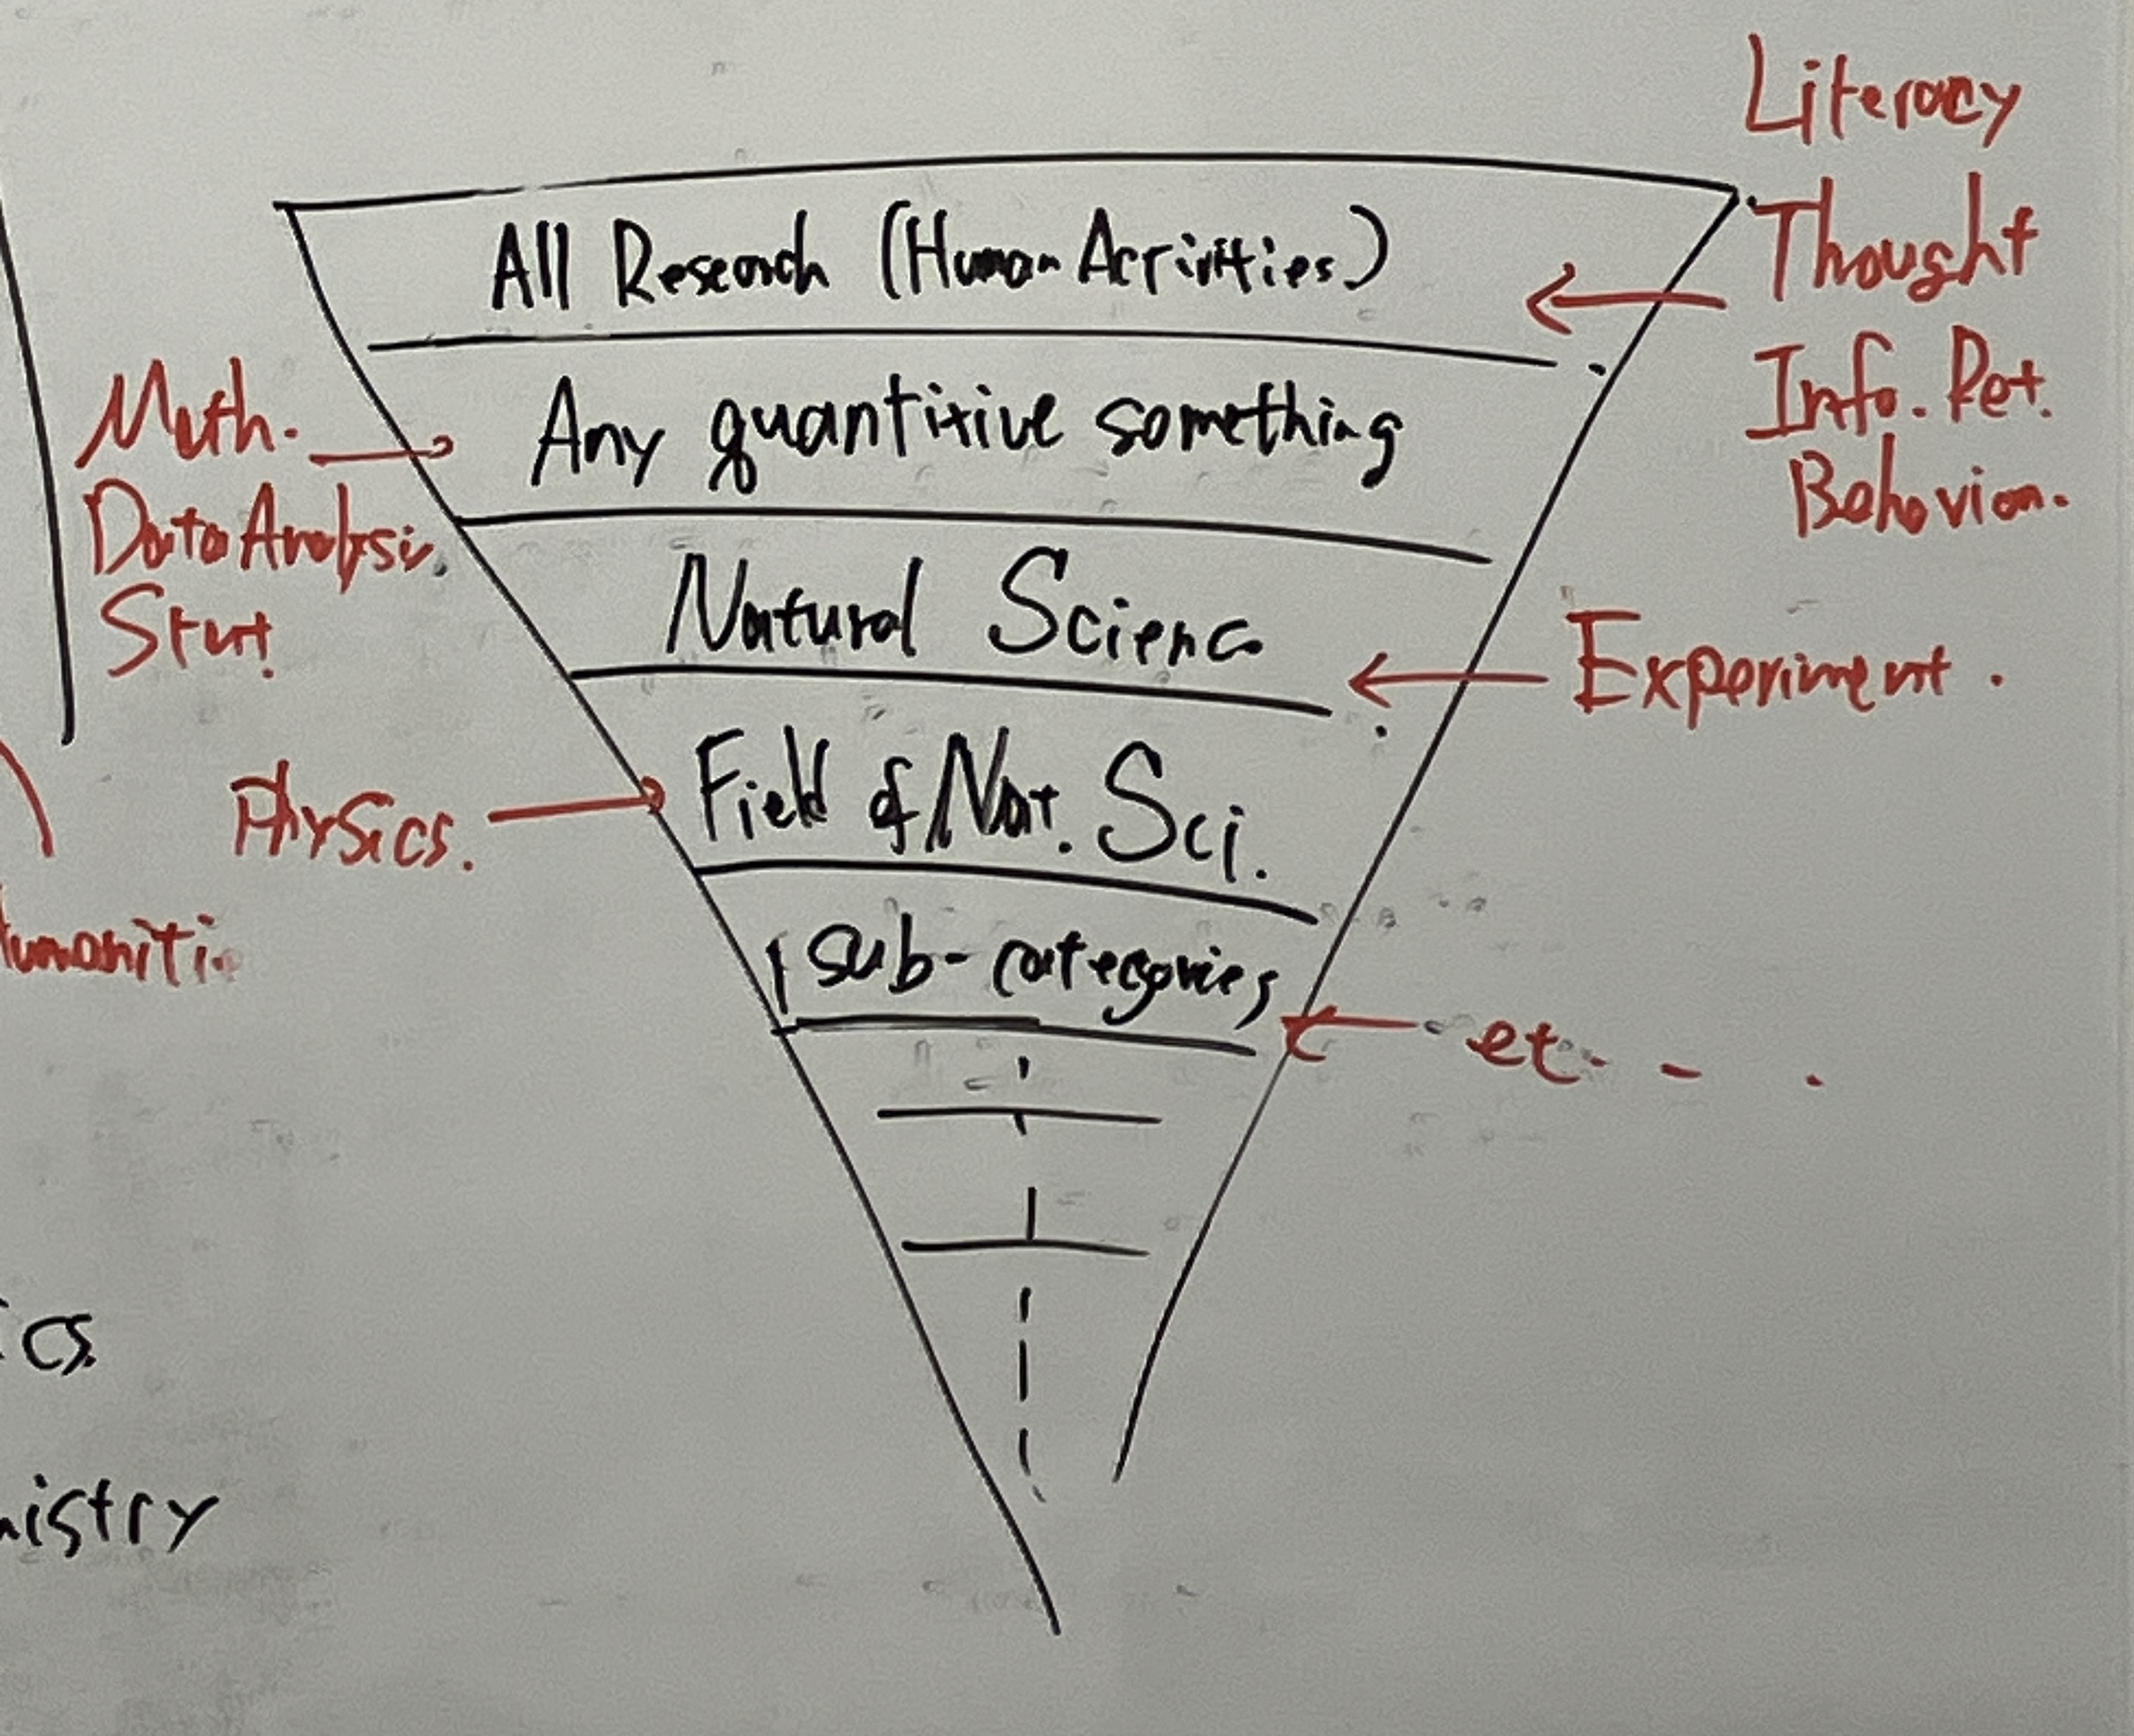
\includegraphics[width=\linewidth]{figs/generality_level.jpg}
    \caption{Caption}
    \label{fig:generality_level}
\end{figure}

% \section{Automation of Tasks for Diverse Field of Research}

% \subsection{Scholarly Document Processing}
% \textit{Scholarly document processing} is a general term for research on automated processing related to scholarly articles and has been studied as part of natural language processing, text mining, and information retrieval.

% \textcolor{red}{TODO: Skip for now. Need reconstruction because many of the issue discussed below are no more issue for research automation. Most of these will moved to Appendix}

% \subsection{Peer Review}
% Many studies have tried to automate peer review generation \cite{thelwall2019artificial,li2019generating,schulz2022future,yuan2022can,yuan2022kid,lin2021automated1,lin2021automated2,kumar2022investigations,bharti2022can,uban2021generating,wang2020reviewrobot}. While not generating peer reviews directly, studies focused on automating research paper assessment  can be said to be related to the peer review automation. \cite{kousha2022artificial,li2020multi,huang2018deep}. These studies have proposed the method to assess the quality \cite{thelwall2022predicting,thelwall2022can}, novelty \cite{pelletier2022novelpy,amplayo2019evaluating,shibayama2020measuring}, soundness \cite{cabanac2022decontamination}, and significance \cite{zong2022citation,xia2023review,soni2022predicting,manghi2021new,soni2021follow,van2020schubert,mckeown2016predicting}.

% These investigations concern the automation of processes occurring subsequent to a manuscript's arrival at the hands of reviewers. Conversely, researchers also have investigated the automation before that process, such as determining the appropriate journal for submission \cite{michail2023journal} and assigning the reviewers \cite{zhao2022reviewer}.

% While not centered on automation, certain studies engage in the scientific analysis of the review process \cite{shah2022challenges,verma2021attend,bharti2022confident,bharti2022betterpr,verma2022lack,kennard2022disapere}. These investigations serve to enhance our understanding of the nature of peer review and, in turn, provide valuable insights for the design of more effective automated review methodologies. 

% \subsection{Cognitive }

% \section{Automation of Tasks for Diverse Fields of Science}
% % There are prerequisite competencies and knowledge required to conduct scientific research. And the question of how to acquire such abilities has been one of the major concerns of AI research for science. Therefore, we will first introduce these research areas. In particular, we will present research on processing scientific literature and understanding scientific knowledge.

% % \subsection{Automated Theorem Proving}



% % \subsection{Understanding Scientific Knowledge}

% % \subsection{AI for Science}

% TODO

% \textcolor{red}{TODO: table for case studies to test the scientific understanding of chatgpt and gpt-4 }

% \subsection{Scientific Machine Learning: Inserting Inductive Bias for Scientific Understanding}
% Another prominent approach to incorporating such scientific knowledge into artificial intelligence is to incorporate inductive biases that help scientific understanding. This area has been studied typically under names such as \textit{scientific machine learning (SciML)} and \textit{physics-informed machine learning}.

% Whereas methods to learn scientific knowledge from the literature are generic methods that learn scientific knowledge through the generic interface of language, in this approach, humans add biases to either the model, the data, or the optimization method that are assumptions of scientific understanding. The constraints that have been studied include the abilities to handle (differential) equations, symmetry, intuitionistic physics, and so on \cite{hao2022physics}. 

% For differential equations, Physics-Informed Neural Networks \cite{raissi2019physics} and Neural Operators \cite{kovachki2021neural} are well known examples of this line of studies. These are methods that enable data-driven simulation of differential equations from data (forward problems) and differential equation discovery (inverse problems). Deep neural networks that can handle symmetry are studied under the name \textit{geometric deep learning} \cite{bronstein2021geometric}. The following survey is comprehensive in this area and should be referred to by those interested \cite{hao2022physics}.

% \subsection{For Empirical Studies}
% Research methods in science can be empirical or non-empirical. Empirical research is research that involves the generation of data, one of the crucial elements in science. Here, we present an effort to automate research on tasks related to scientific data. Machine learning is used in these areas in a variety of ways, including variable selection and model selection, but this section will focus specifically on those areas that have names.

% \subsubsection{Laboratory Automation}
% \textit{Laboratory automation} is a program that seeks to automate empirical research involving scientific experiments that involve interaction with the physical world.

% What makes this effort unique compared to other efforts to automate research is that it seeks to automate the entire process of validation, and it seeks to automate even the manual labor of humans in experimentation. Specifically, they automate human tasks by creating robots that can conduct research. A few examples include ``Mahoro'', a general humanoid robot that can conduct various experiments \cite{yachie2017robotic}. The robot could automatically conducted cell culture tasks using \cite{ochiai2021variable}

% \subsubsection{Bayesian Experimental Design}
% In order to conduct an efficient experiment, it is necessary to properly determine which experimental. \textit{Experimental design}, which involves devising efficient methods for conducting appropriate experiments, has long been studied. \textit{Bayesian experimental design} is an attempt to optimize and automate this experimental design by using Bayesian optimization \cite{chaloner1995bayesian,shahriari2015taking}. Bayesian experimental design has been incorporated from a relatively early stage and has been used in materials science and other fields.


% \subsubsection{Symbolic Regression / Equation Discovery}
% % \subsubsection{Symbolic Regression} 
% Scientists have constructed models in the form of mathematical equations that explain them from observational data. This has enabled us to go beyond observational data to understand and predict underlying phenomena. That is to say, formulating a mathematical representation that elucidates the phenomenon behind the data is an extremely critical step in science. 

% % Modern science is composed of a cycle of observation, hypothesis generation, and hypothesis testing. In many fields, including physics, chemistry, and biology, mathematical models are often constructed as hypotheses from observational data. 

% One attempt to automate this endeavor is \textit{symbolic regression} \cite{makke2022interpretable}, or \textit{equation discovery}. These are attempts to infer from the data a formula that explains it. While classical approaches to symbolic regression have traditionally employed methods such as evolutionary computation, recent years have seen the emergence of strategies utilizing deep neural networks \cite{petersen2019deep,udrescu2020ai,udrescu2020ai2,cranmer2020discovering,kamienny2022end,d2022deep}. Some researchers have proposed the frameworks \cite{landajuela2022unified,keren2023computational} and benchmarks \cite{matsubara2022rethinking} for symbolic regression. You can find a literature review of symbolic regression in \cite{makke2022interpretable}, and that of the early studies in \cite{kramer2023automated}.

% % \subsection{Knowledge Representation and Reasoning}

% \section{Automation of Tasks in Each Research Field}

% It has become commonplace to streamline domain-specific tasks in scientific research using machine learning, resulting in a vast number of published papers. Even just to mention a few that come to mind, there are studies on molecular biology \cite{jumper2021highly,senior2020improved}, material science \cite{ramprasad2017machine}, medical science \cite{vamathevan2019applications,shorten2021deep}, quantum mechanics \cite{carleo2017solving}, cosmology \cite{carleo2019machine}, genetics \cite{libbrecht2015machine}, and nuclear physics \cite{degrave2022magnetic}. It is impossible to cover all of these applied studies of research automation of science. Therefore, in this paper, we will not go into detail about each of these studies. Instead, we will present research on automation of elements that can be applied in various fields of science. For the literature survey of domain specific automation, please refer to \cite{xu2021artificial}. \textcolor{red}{TODO: Add application studies}

% \subsection{Automating Machine Learning}

% \subsubsection{AutoML}
% AutoML is an attempt to automate all tasks associated with machine learning. This includes hyperparameter optimization, model selection, and automation of various pre- and post-processing steps. The following website \cite{automlorg} provides a very active overview of AutoML. The book \cite{hutter2019automated} for an overview of AutoML through 2019, the paper \cite{bischl2023hyperparameter} for hyperparameter selection, and \cite{lindauer2020best,white2023neural} for the current state of the NAS are very helpful to catch up to this field.

% \subsubsection{MLOps}
% MLOps (Machine Learning Operations) is a general term for efforts to streamline and automate operations related to machine learning in industry. For example, it includes automating tasks such as model deployment and continuous training, as well as experiment management. To be sure, many MLOps solve problems in industry, and not all of them are related to research automation. However, when actually conducting research, we are involved in experiment management, versioning, and other tasks. While research on research automation has left out automation of these tasks, MLOps is accumulating knowledge on automation of these tasks as well.  The paper \cite{kreuzberger2023machine} is a good scientific review paper on MLOps.

% 
\tikzstyle{my-box}=[
    rectangle,
    draw=red,
    rounded corners,
    text opacity=1,
    minimum height=1.5em,
    minimum width=5em,
    inner sep=2pt,
    align=center,
    fill opacity=.5,
]
\tikzstyle{leaf}=[my-box, minimum height=1.5em,
    fill=orange!20, text=black, align=left,font=\scriptsize,
    inner xsep=2pt,
    inner ysep=4pt,
]
\begin{figure*}[tp]
    \centering
    \resizebox{\textwidth}{!}{
        \begin{forest}
            forked edges,
            for tree={
                grow=east,
                reversed=true,
                anchor=base west,
                parent anchor=east,
                child anchor=west,
                base=left,
                font=\small,
                rectangle,
                draw=red,
                rounded corners,
                align=left,
                minimum width=4em,
                edge+={darkgray, line width=1pt},
                s sep=3pt,
                inner xsep=2pt,
                inner ysep=3pt,
                ver/.style={rotate=90, child anchor=north, parent anchor=south, anchor=center},
            },
            where level=1{text width=5.6em,font=\scriptsize,}{},
            where level=2{text width=5.6em,font=\scriptsize,}{},
            where level=3{text width=5.5em,font=\scriptsize,}{},
            where level=4{text width=6.1em,font=\scriptsize,}{},
            [
                AI for Research, ver
                [
                    Natural Science, ver 
                    [
                            \cite{zhang2023artificial}{,}
                            \cite{xu2021artificial}{,}
                            , leaf, text width=46.8em
                    ]
                    [
                        Physics
                        [
                            \cite{carleo2017solving}{,}
                            \cite{carleo2019machine}{,}
                            , leaf, text width=39.7em
                        ]
                    ]
                    [
                        Chemistry
                        [
                            \cite{coley2020autonomous}{,}
                            , leaf, text width=39.7em
                        ]
                    ]
                    [
                        Biology
                        [
                            \cite{libbrecht2015machine}{,}
                            , leaf, text width=39.7em
                        ]
                    ]
                    [
                        Med. Science
                        [
                            \cite{vamathevan2019applications}{,}
                            \cite{shorten2021deep}{,}
                            , leaf, text width=39.7em
                        ]
                    ]
                ]
                [
                    Formal Science, ver
                    [
                        Mathematics
                        [
                            \cite{rabe2021towards}{,}
                            , leaf, text width=39.7em
                        ]
                    ]
                    [
                        Comp. Science
                        [
                            Contrastive~\cite{chalmers2013thing}{,}
                            POTTER~\cite{chalmers2013thing}{,}
                            CoT~\cite{chalmers2013thing}{,}
                            MCR~\cite{yoran2023answering}
                            , leaf, text width=39.7em
                        ]
                    ]
                ]
            ]
        \end{forest}
    }
    \caption{Review Paper of AI for Resear}
    \label{fig:categorization_of_reasoning_big}
\end{figure*}


% % \section{Another Axis: Research Process}
% % We have presented the idea that attempts to automate research could be classified hierarchically according to how broadly they could affect research. In addition to this, we believe that these efforts can also be categorized from another angle. That is, from the perspective of what part of the research process is being automated. For example, one effort might automate only the hypothesis generation part of a broad scientific study, while another effort might automate the entire research process instead of focusing on a specific research question. Also, for example, within an effort to automate validation, one effort might automate experimentation, another might automate proofs, and yet another might automate both of these. Thus, the second axis is what part of the research process is being automated and to what degree of generality.

% % Along this second axis, we will review our efforts in research automation. However, since there are a vast number of examples of research automation even in one sub-process, e.g., hypothesis generation, we will not go into individual details, but rather give priority to conveying the big picture.

% % % \textcolor{red}{NOTE: touch briefly do not go too specific, just show interpretation}
% % % \section{Knowledge Production}
% % % The Process of Creating New Knowledge

% % % Modern research is constructed from three main phases: observation, hypothesis generation, and hypothesis verification <- not line but cycle

% % \subsection{Question Construction}
% % In research automation studies, questions are often given. An exception is research that automatically discovers questions and issues from the academic literature. For example, Lahav et al. have proposed a methodology for automating the discovery of prevailing challenges within the research community, as well as the emerging hypotheses to address them \cite{lahav2022search}.

% % \subsection{Hypothesis Generation}
% % It is probably fair to say that hypothesis generation is one of the most common processes studied in research automation. Prediction of 3D structures from amino acid sequences, prediction of material structures from desired physical properties, and prediction of newly applicable disease candidates from existing drugs, just to name a few, are examples of automated hypothesis generation. In the example given in the previous section, symbolic regression is another example of hypothesis generation. These studies are often aimed at automation and optimization to solve bottlenecks in problems specific to each research area.

% % \subsubsection{Hypothesis Generation from Scientific Papers}

% % One study of automated hypothesis generation that is generic to a wide range of fields is the automatic generation of hypotheses from scholarly literature. In recent years, several researchers have presented studies on automating scientific analogical reasoning for identifying the relationship between problems and their corresponding solutions \cite{kang2022augmenting,chan2018solvent}, which is hypothesis.

% % % For example Portenoy proposed a system that recommend researchers who are pursuing analogous research objectives via divergent approaches \cite{portenoy2022bursting}.el techniques.

% % % \subsubsection{Others} 

% % Some methods have been proposed that don't generate hypotheses directly, but rather assist humans in generating hypotheses from experimental data 
% %  \cite{friederich2021scientific}.

% % \subsection{Hypothesis Verification}
% % Attempts to automate the verification of hypotheses include Bayesian experimental design, laboratory automation, and automated theorem proving, if theorems are viewed as hypotheses, as mentioned above. For example, some researchers have tried to automate experimental design for quantum physics \cite{ruiz2022digital} or proposed to design workflow of scientific research as a software \cite{goble2020fair}. Others have proposed machine learning algorithms for formulating and executing experimental designs in a more abstract and simple manner \cite{herrmann2022learning}. 

% % % \subsubsection{Verification Design}

% % % Once a hypothesis is formulated, a plan is developed to test its validity. The design of this verification plan is far more flexible than that of hypothesis generation, making it more difficult to handle uniformly. To be more precise, while many sciences have standardized methods such as statistical tests for verification, there is a wide variety of methods for generating the data used for the verification. One study may require a huge machine to collide elementary particles, while another may use rats for behavioral experiments. Some studies may require the use of chemicals, while others can be simulated on a computer. Furthermore, even with standardized statistical tests, as mentioned earlier, automating their creation from scratch proves exceedingly challenging. It is readily apparent that devising standardized methodologies like statistical tests is difficult when one must not merely employ them as tools but also contemplate the very nature of what it means to verify, as well as the rationale behind adopting specific assumptions. Therefore, it may not be an overstatement to say that this aspect represents the biggest obstacle towards achieving complete automation of research in a unified manner.

% % % \subsubsection{Verification Execution}

% % % Once a verification plan has been devised, the process proceeds in accordance with it. As previously mentioned, the approach may vary considerably. However, in many scientific methodologies, statistical techniques are employed. In these instances, the verification process can be broadly divided into two stages: 1. data generation and 2. analysis of the generated data for verification.

% % % As previously mentioned, data generation methods span a wide range. Among these, attempts have been made to automate the work of researchers within laboratories, an endeavor known as Laboratory Automation. For instance, 
% % % some studies focus on automating cell culture tasks using humanoid robots \cite{ochiai2021variable},
% % % TODO: add more

% % % TODO: may differentiate the analysis for hypothesis generation from that for verification
% % % we interpret data processed according to a certain criterion, assessing the validity of our inferences. Here, we make an explicit distinction between analysis for verification and analysis for hypothesis generation. Modern science is composed of a cycle of observation, hypothesis generation, and hypothesis testing. It's common to generate the next hypothesis to be tested from data produced for verification. However, this merely signifies that we conduct both hypothesis generation and testing through a somewhat inductive reasoning based on data. Therefore, in this context, we will focus on data analysis for hypothesis testing, while data analysis for hypothesis generation will be included in the hypothesis generation section introduced earlier.

% % To validate the plausibility of assertions, we currently employ statistical methods. There is research that automate the hypothesis testing \cite{gil2016automated}. 

% % Some researchers have engaged on automating data visualization and analysis \cite{bavishi2021vizsmith,bavishi2022tools}.

% % \subsubsection{Scientific Claim Verification}

% % Compared to question construction and hypothesis generation, there are few attempts to automate hypothesis verification related tasks from the academic literature. Somewhat related is the field of \textit{scientific claim verification} \cite{li2019scientific,wadden2020fact,wadden2022scifact,wadden2022multivers}, which determines the validity of a scientific claim through analysis of research paper. This is not the planning or execution of validation, but it is related to the automation of validation in the sense that it seeks to understand the validity of scientific claims. Since it is an assessment of the validity of a study, the findings of this study may have implications for the automation of peer-review.

% % \subsection{Pipeline (All Process)}
% % Most research on research automation automates some tasks in the research process. In contrast, there are attempts to automate the entire research process from start to finish.

% % \subsubsection{Self-Driving Labs}

% % A seminal early works are Adam \cite{king2004functional}, and Eve \cite{williams2015cheaper}. These are closed-loop scientific discovery systems that autonomously execute everything from hypothesis generation to research planning. These systems have logic AI at their foundation. The author of the paper of Adam call these system \textit{robot scientists}, \textit{self-driving labs}, \textit{autonomous discovery}, or \textit{laboratory automation}.

% % \subsubsection{Scientific Workflow}

% % Additionally, the concept of a \textit{scientific workflow}, which represents data and computational processing pipelines in research as software, emerged in the early 2000s. The developments and advances in research related to scientific workflows are consolidated in this literature \cite{barker2008scientific,atkinson2017scientific}. Additionally, these papers \cite{deelman2019role,nouri2021exploring} discusses how machine learning contributes to streamline the each step in the scientific workflow. These are important initiatives in terms of softwareizing the research process \cite{deelman2015pegasus,gil2011semantic}.

\subsubsection{Autonomy}

\subsubsection{General and Autonomous AI}

So far we have introduced the idea that we can look at research automation from two axes: the ``research field'' axis and the ``research process'' axis. We will try to paint a conceptual picture of how research automation can be viewed from these two axes.

\begin{figure}[htb]
    \centering
    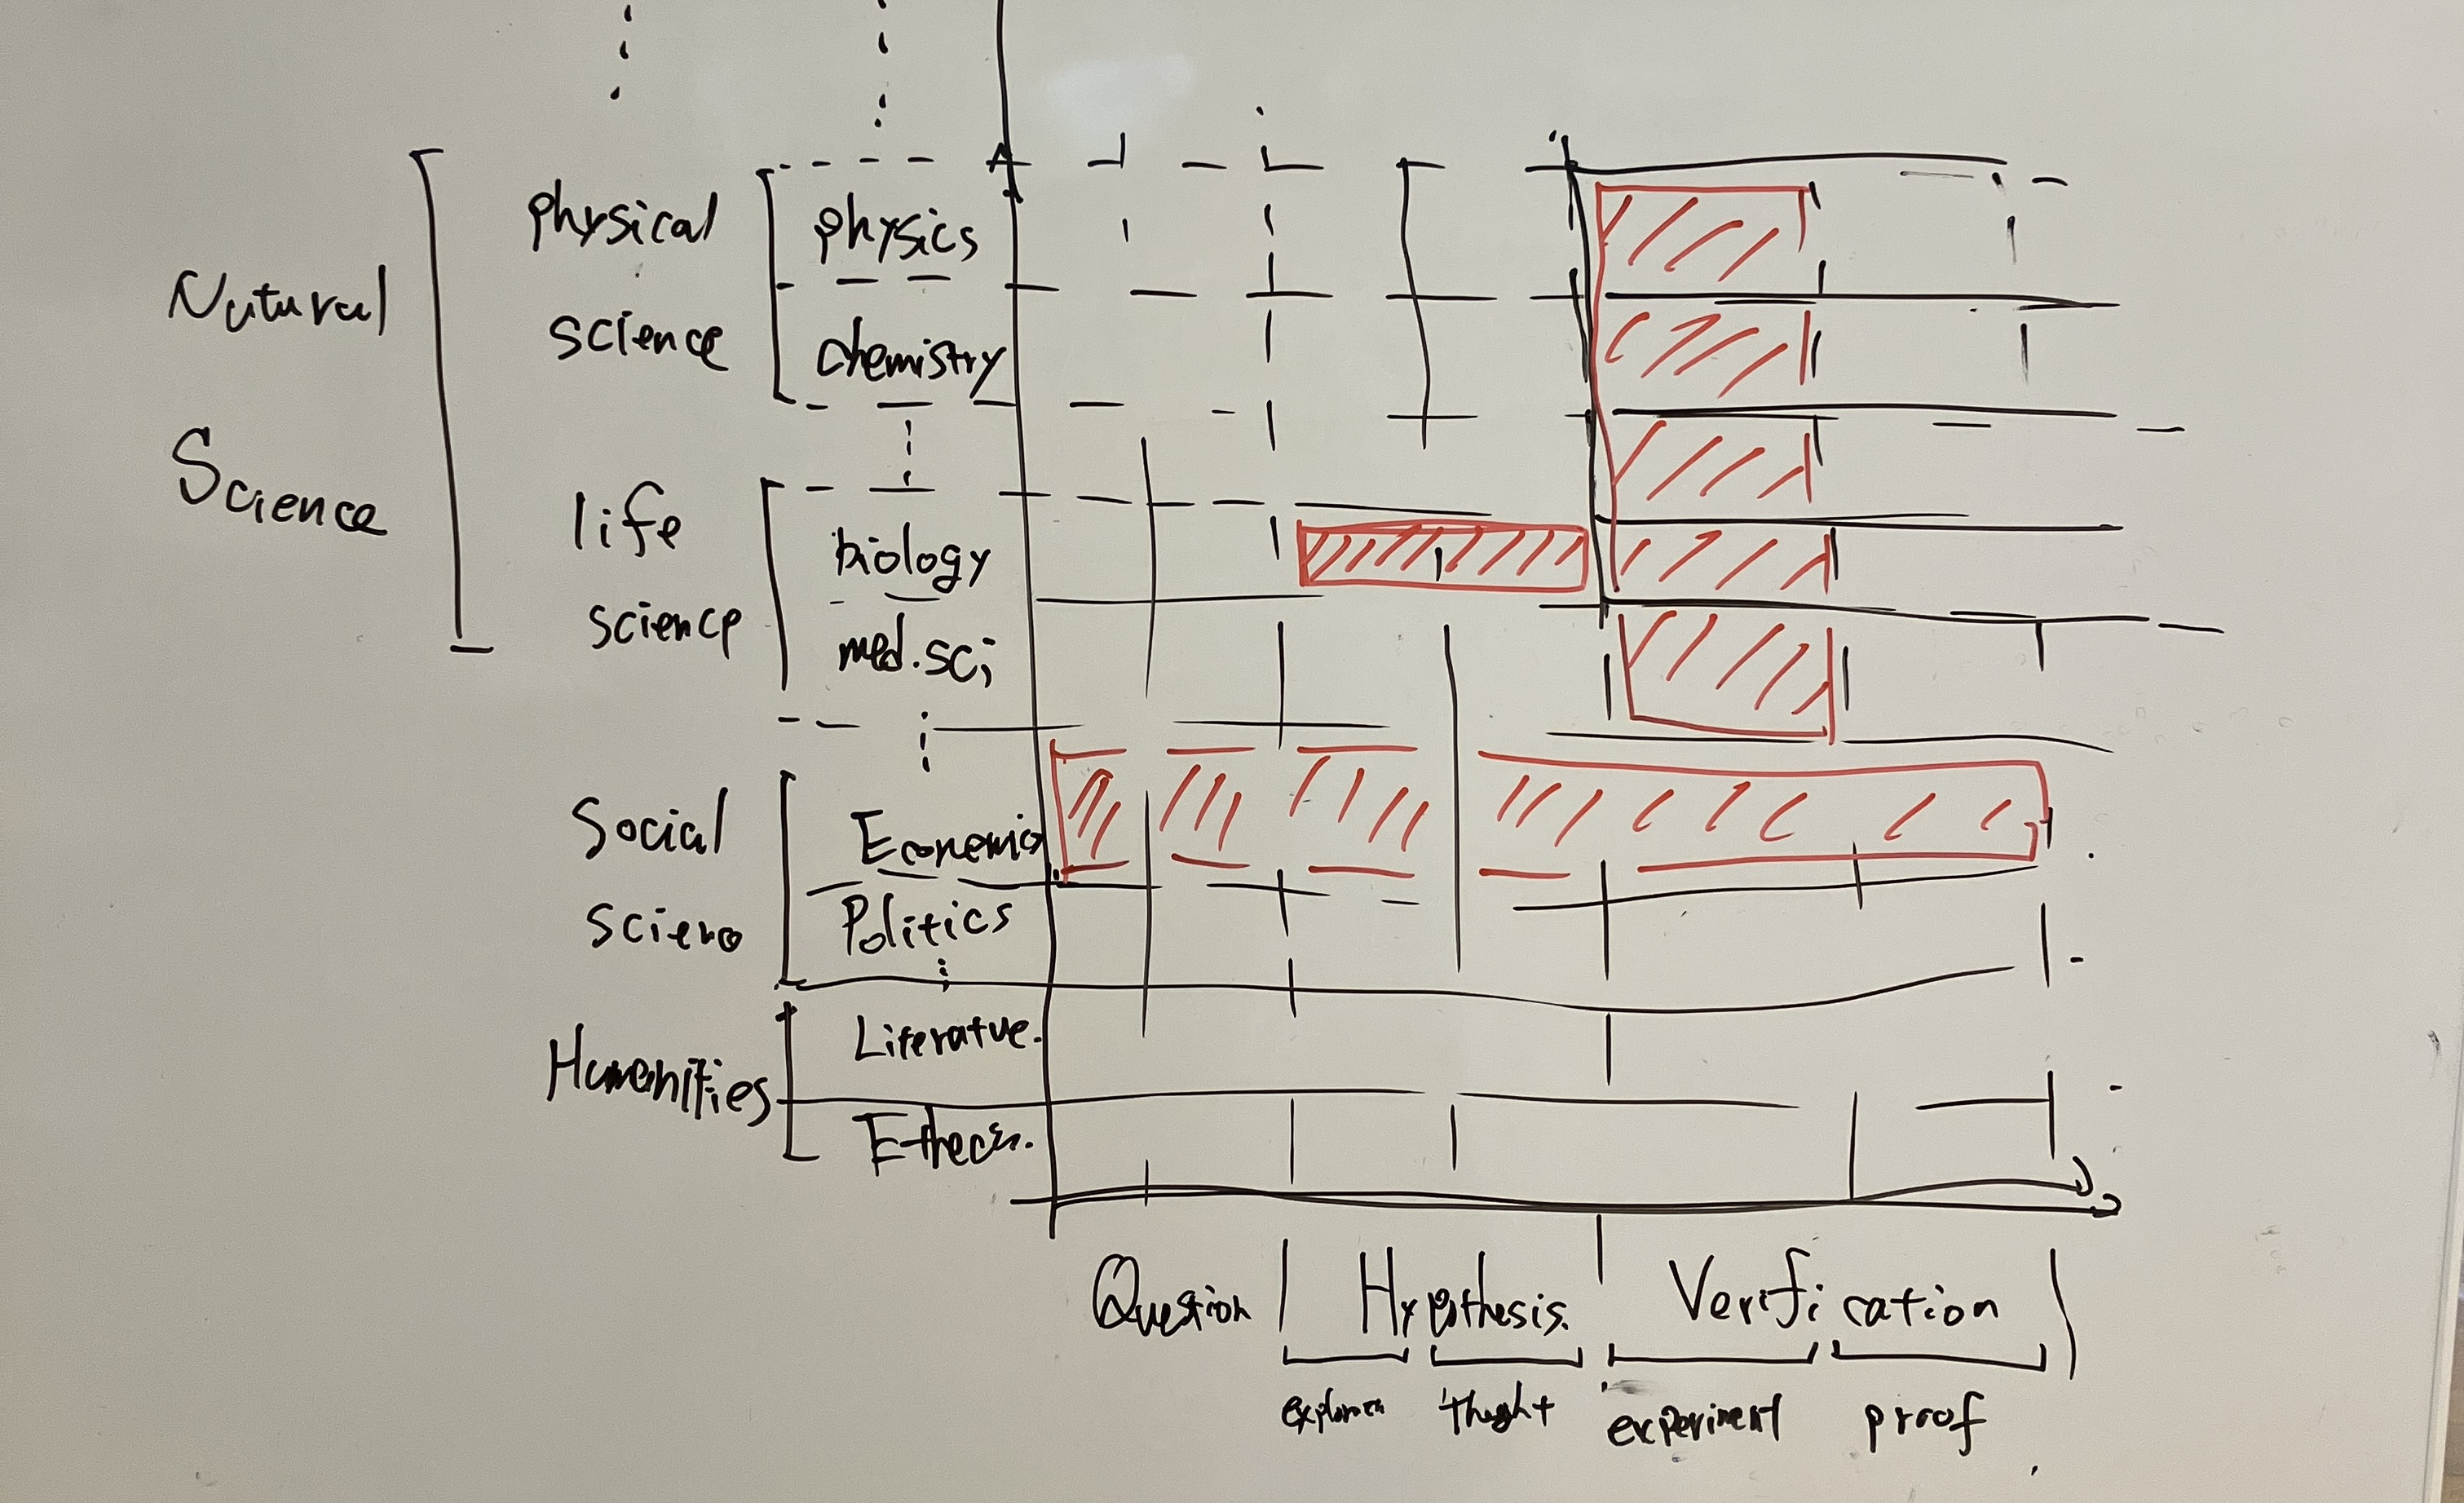
\includegraphics[width=\linewidth]{figs/generality_matrix.jpg}
    \caption{Caption}
    \label{fig:generality_matrix}
\end{figure}

Fig. \ref{fig:generality_matrix} conceptually illustrates the position of automation according to the axes of research field and research process. The vertical axis is the research field axis and the horizontal axis is the research process axis. Closer to the vertical axis corresponds to more specific research areas, and farther away from the vertical axis corresponds to a broader range of research areas. The horizontal axis corresponds to question construction, hypothesis generation, and hypothesis testing, from left to right, and is further divided within each category into more detailed e.g. empirical and non-empirical methods. Note that this is only a conceptual diagram and not an exact classification.

As a example, the automation of protein structure prediction \cite{jumper2021highly} can be seen as the automation of a certain hypothesis generation task in a certain molecular biology study. The work of robot scientist \cite{king2004functional} can also be understood as an attempt to automate many of the steps in the study of identifying the function of genes in genetics, from hypothesis generation, to testing, to generating new hypotheses. (Explanation of the figure).

Our goal of creating a versatile and autonomous artificial researcher is to automate everything on this two-dimensional surface. The area circled by the blue qualification in this figure corresponds to that. In other words, our goal is to realize an artificial intelligence that can autonomously execute any research or any process of research.



% \section{Others}

% Upon the completion of a study, the drafting of a manuscript, and its successful navigation of the peer-review process, the resulting findings are deemed to possess a degree of credibility as knowledge. Naturally, it would be hasty to assert that this alone births ``correct'' knowledge, as research demands iterative verification to confirm its validity. We convey such knowledge to others through various means, one of which is the presentation of research findings. To effectively communicate these outcomes, we create slides that elucidate our work. Studies also exist that strive to automate this aspect of the dissemination process \cite{sefid2019automatic}.

\section{Conclusion}
\chapter{Challenges and Propositions}
In Chapter 2, we examined the definition of research and its implications, and in Chapter 3, we provided an overview of past efforts related to the automation of research. In this chapter, based on these, we will reorganize the challenges towards realizing an autonomous and general artificial intelligence capable of conducting research.



\section{Challenges}

 \subsection{General and Autonomous Question Construction, Hypothesis Generation, and Hypothesis Verification}

 In Chapter 2, we explained that in order to create an AI capable of conducting any research, it is deemed necessary to realize the formulation of questions, generation of hypotheses, and validation of these hypotheses as a combination of universal skills applicable to all research. In this section, we will revisit and organize the potential challenges in achieving an AI that can conduct each of these processes.

 \subsubsection{Common Challenges}
One of the major challenges that can be a common issue for any process, as pointed out in prior research \cite{coley2020autonomousII}, is how to execute these tasks in open-ended situations. For instance, in the automation of experiments, robots use experimental equipment selected, prepared, and set up by humans. However, humans do these tasks from scratch with their own hands. Humans do not use a given corpus of papers; instead, they search for and use them on their own. Candidates for hypotheses are not explicitly provided; humans begin by identifying potential hypotheses. Even when formulating questions that serve a particular goal, humans set that goal themselves. 

In many cases in research automation, these elements are pre-determined by humans. How to let machines autonomously perform these tasks starting only with the same initial information given to humans is crucial in realizing an autonomous artificial researcher. Moreover, having this kind of freedom is essential to achieving a general artificial researcher as well. This is because if we impose constraints on AI to research only within specific research questions or hypothesis spaces defined by humans, it cannot become an AI capable of conducting arbitrary research. Therefore, a significant challenge is how to make AI acquire complex foundational skills and fundamental reasoning abilities to realize these capacities.

\subsubsection{Question Construction}

The first issue discussed in Chapter 2 is the problem of determining the unknown nature of the answer to a question. Given that research is an endeavor to produce new knowledge, it is necessary for the answer to the question to be unknown. Therefore, there is a need to generate such questions or later verify that the answer to the question is indeed unknown.

The second challenge is the issue of how to make a machine generate a ``good'' question. Firstly, what researchers consider as a ``good'' question is not always consistently agreed upon among them. Furthermore, we pointed out that the ``goodness'' of a question is inherently a concept relative to the individual or society. Hence, there seems to be a need to clearly define what constitutes a good question and think about how to effectively integrate these definitions.

The third challenge is that as we demand more autonomy from AI, the automation of question formulation becomes more difficult. Inherently, questions are constructed based on various motivations, such as pure intellectual curiosity or for specific objectives. It is very challenging to automate the construction of questions without defining which of these motivations should be the source. Moreover, as mentioned in Chapter 2, the construction of questions encounters the problem of infinite regression when pursued with strict autonomy. Even if not taken to that extreme, setting higher-order objectives behind questions for AI is an exceptionally difficult task.

It seems that the automation of question formulation has received relatively less attention compared to other processes. Since the formulation of questions is an essential element in conducting research, it would be desirable for more focus to be directed towards the research on automating this process.z

% Realizing AI that construct a ``good'' question in a generic way is challenging. As discussed in Section \ref{section:the-relativity-of-knowledge-production-to-society}, research is relative to society and different criteria can be considered for what makes a ``good'' question. Thus, some human perspective on the ``goodness'' of a question must be incorporated. We need to discuss what we consider good, what we should prioritize, and how to incorporate the value to AI.

% \textcolor{red}{TODO}

% Moreover, determining inputs to the question construction module is not trivial. In hypothesis generation, the question is the primary input, whereas in verification, it's the hypothesis. However, question formation take any input. Once you seriously try to identify the origin of question, you will encounter infinite regress. This is a unique problem that arises when aiming for a general-purpose and autonomous artificial researcher. This is because the issue revolves around how much input can be assumed while still being considered autonomous, given that it can potentially take any input.

% \cite{wang2023skillqg}

% neural question generation \cite{pan2019recent}


\subsubsection{Hypothesis Generation}

One challenge in creating an intelligence capable of hypothesis generation, not just as a tool for humans, is the need to empower the machine itself to form plausible hypotheses for questions to which even the machine doesn't know the answer. Current machine learning models have been criticized for potentially not knowing what they don't know \footnote{
In our discussion with Wataru Kumagai, we were reminded once again of the importance of self-awareness in creating an AI capable of conducting research.
}. 
Moreover, they are known to confidently provide answers or fabricate falsehoods about topics they are ignorant of. Therefore, it seems essential to first accurately recognize what is unknown, either for oneself or the world at large, as told in sections of question construction. Upon facing an unknown subject, there's a need to reduce uncertainty and approach understanding. As mentioned in Chapter 2, humans attempt to understand uncertain subjects by gathering information from papers, experiments, or by reframing questions. While it may not be necessary to adopt the exact same approach, it seems essential to enable machines to autonomously adopt strategies to reduce uncertainties.

% Outputs from machine learning models are essentially inferences tinged with uncertainty. From this perspective, one could posit that these models are already inherently generating hypotheses. Indeed, they are already employed for hypothesis generation in numerous scientific investigations.

% However, while these hypotheses might be hypotheses in the sense that the answers are unknown to humans, they might be self-evident to the machine learning model. When we talk about AI generating hypotheses in the context of AI conducting research, the ultimate expectation is for the AI to provide plausible answers to what is unknown to AI itself. This remains an unresolved issue.

As one of the promising approaches for tacking unknowns, it seems crucial for AI to acquire systematic thinking to realize this, as humans developed systems like language and mathematics, allowing them to infer about subjects beyond their experience. Systematic thinking is not only important for out-of-distribution generalization but is also valued for interpretability, causal inference, logical reasoning, mathematical processing, and planning.

\textcolor{red}{TODO}

\subsubsection{Hypothesis Verification}

In Chapter 2, we highlighted several challenges in realizing an AI capable of verification. First and foremost, the AI itself needs to understand what verification is, and by what criteria a sequence of actions qualifies as verification. Ideally, it would be preferable for the AI to contemplate and understand from scratch what verification is. However, many humans don't do this either, and as discussed in Chapter 2, the philosophical debate on precisely defining verification is still unresolved. Therefore, it's harsh to demand this of a machine. At the very least, the machine needs to thoroughly understand and proficiently use verification concepts that humans employ, such as statistical hypothesis testing, from first principles.


Second, the AI must be able to formulate detailed and complex plans to verify a hypothesis. With the advancements in language models in recent years, we are now much more capable of formulating superior plans than before. However, devising detailed plans remains a challenging issue.

Third, it has to be prepared to carry out these plans and execute the plan with the combination of human-like complex actions.As mentioned in Chapter 2, to achieve this, the AI must be able to search for, create, purchase, and manipulate equipment with almost the same degree of freedom as humans, requiring it to exhibit extremely sophisticated and complex behaviors. This is an immensely challenging issue, and it might even be fair to say it's one of the biggest bottlenecks in realizing an intelligence capable of generic and autonomous research. Laboratory automation have attempted to address this challenge in real world by developing robots. We will discuss the case within the computer below.

For AI to execute research on a computer, it must perform any operation within the computer. For instance, machine learning research entails, setting an environment, preparing datasets and models, and writing and executing codes. To allow AI to prepare these without human intervention, the AI itself must be able to autonomously search the web, select data, download it, and so on. Furthermore, once the AI generates code for verification, it must operate the shell to execute it.

There are ongoing initiatives to enable language models to operate browsers \cite{nakano2021webgpt,act1}. While full browser operations might seem ambitious, there are already endeavors to allow language models to conduct searches \cite{mialon2023augmented}. If we achieve browser automation, it will greatly advance research automation involving web operations. Moreover, efforts like the open interpreter \cite{openinterpreter} aim to automate any computer action. This direction holds promise for automating all research confined within a computer. Although these studies are gaining traction in the machine learning domain, they're not always linked to research automation. We advocate recognizing this as a pivotal challenge in the realm of research automation.

In the field of machine learning, it seems that the discussion on automated validation has not garnered much attention until now. However, recently, the need for verification is recognized in the machine learning community beyond outside of the context of research automation. Studies like \textit{scientific claim verification}, which received much attention during the COVID-20 pandemic \cite{wadden2020fact}, or attempts to minimize hallucination \cite{dhuliawala2023chain} are examples of them. These are not attempts to automate validation in research. Therefore, these findings cannot be directly applied to the automation of research validation. However, we expect that these studies will provide useful insights for the future development of artificial intelligence capable of understanding validation.

% Creating AI that autonomously verifies hypotheses is challenging. While current models can mimic human verification, truly understanding the verification strategy demands more work. Sometimes, they even need to devise the verification measure themselves.

% The biggest challenge for autonomous verification is the need to freely move around in the real world or within a computer, and to manipulate objects within that world at will. We believe this to be one of the greatest barriers to full research automation. Laboratory automation have attempted to address this challenge in real world by developing robots. We will discuss the case within the computer in Section \ref{section:behaviour-inside-the-computer}.

% \subsubsection{AI Capable of Peer Review}

% Given the difficulty of these challenges, automating peer review could be a strategic starting point. This is because peer review is a universal process across diverse research fields and it assesses the validity and quality of problems, hypotheses, and verification methods, which is easier than generating them. Despite some progress, full automation is still elusive \cite{yuan2022can,schulz2022future}.


% \subsection{Behaviour inside the Computer}
% \label{section:behaviour-inside-the-computer}


% Lab Notebook?
% \subsection{Dataset of Research Process}
% It is important to establish the necessary infrastructure for research automation. The two pillars of research automation are the development of basic models that incorporate academic knowledge and the construction of data sets. The development of an infrastructure model that incorporates scientific knowledge has already been proposed in many places and is actually under development, so I will not emphasize its necessity here again. Also, regarding data sets, the construction of data sets for the acquisition of scientific knowledge has been done in various places as well, so I will not emphasize that here either.

% Instead, we propose here to construct a research process dataset. A research process dataset is behavioral log data that incorporates all possible tasks throughout the entire process of the study, from start to finish. Ideally, individual tasks should be labeled as to whether they correspond to question construction, hypothesis generation, or hypothesis testing. We believe that building such a data set is important because, as explained in the Literacy section of Chapter 2, the current paper is not a data log of the entire research process. This makes it difficult to be data-driven and end-to-end learning how to do research itself. I believe that building a research process will help solve these problems and increase the likelihood of more flexible intelligent agents.

% However, building a dataset of the research process seems daunting. This is because researchers who do not currently keep research logs would have to go to the trouble of recording their research process.\footnote{
% In an experimental laboratory in the natural sciences, it is common to take research notes, so it may not be that difficult to record more detailed processes as an extension of this practice. However, in the machine learning field, the culture of taking research notes does not seem to be that common. (We think it is common to keep logs of experiments, but it seems to be rare to describe the details, for example, where and how the data was obtained.) 
% } Therefore, it seems necessary to devise a way to make it easier for researchers to keep logs. It may be to manage the research process on GitHub, or to take research notes as in natural science research, but it is important to discuss how to achieve these things.

% Being able to construct a dataset of the research process would be ideal, but may not be immediately feasible. As an alternative, it seems important to create a dataset designed to automate question construction, hypothesis generation, and hypothesis testing. At its simplest, one might start by building a dataset of papers labeled with the parts that correspond to the question, hypothesis, and test, respectively. This would be a relatively simple but important step in achieving a generic artificial researcher.

% Alternatively, instruction tuning could be done by viewing question construction, hypothesis generation, and hypothesis testing as tasks, respectively. This would produce a language model that can execute question construction, hypothesis generation, and hypothesis testing with greater fidelity. This could be the foundation for a general-purpose, autonomous artificial researcher.



\subsection{Alignment}
As discussed in Section 2, when realizing an AI that autonomously conducts research, the issue of alignment arises. 

First and foremost, it is essential to consider ways to ensure that AI does not engage in research that could harm humans. However, this is a challenging issue. The problem of ensuring that AI does not harm humans is a difficult problem in AI Alignment. Furthermore, knowledge and technology produced by research are fundamentally value-neutral. That is, the knowledge can be used for good or ill. Therefore, even if AI were to research with harmful intentions, it would be challenging to judge from the actual research results.

The remaining two issues arise in the ultra-long term when AI becomes fully autonomous in conducting research. The second issue is that to enable meaningful knowledge production for humans, there needs to be an alignment between the knowledge systems of AI and humans. As mentioned in Chapter 2, if knowledge and verification are relative concepts to society, research conducted autonomously by AI may become meaningless to humans. On the other hand, if we were to correct AI to follow human methods entirely, we might unnecessarily limit the machine's potential capabilities. Deciding how much human methodology and values to incorporate and how much freedom to allow the machine, and finding ways to achieve this, will be a significant challenge in creating research-capable AI.

The third issue concerns the alignment between AI and nature, not between humans and AI. As mentioned in Chapter 2, the fact that humans have come to understand nature is likely not unrelated to our long history of interacting with nature. It seems there's no guarantee that artificial machines like AI, which lack such experiences, would lead to an understanding of nature through their autonomously generated knowledge.

The latter two issues are problems that only arise when demanding extreme autonomy from machines and are not immediately problematic. However, when discussing the limitations and possibilities of knowledge production and natural understanding by agents independent of humans, they seem to become relevant issues.

% In the medium to long term, it's essential to devise ways to ensure that AI doesn't engage in research that could be dangerous to humans. 

% In the long term, we must contemplate how to construct a knowledge system that are mutually translatable between human society and AI society. While these issues may not arise in the short term, it's crucial to engage in discussions now, looking towards the long-term future.

% \subsubsection{Understanding}

% Extensive discourse transpires concerning scientific discoveries. Yet, discussions pertaining to scientific comprehension remain relatively unexplored. Krenn et al. delve into the conundrum of what it entails for a machine learning agent to not only unearth scientific knowledge but also to comprehend it \cite{krenn2022scientific}. They adopt a human-centric stance, positing that an agent's ability to offer explanations comprehensible to human scientists signifies the existence of its scientific understanding.

sun-rise \cite{leslie2023does}

\section{Constructing Research Pipeline Prototypes}
We propose to start by building a research pipeline, connecting the modules of the knowledge production system. The research pipeline is a software system that takes input and generates knowledge as output, encompassing the sequence of processes involved in research. Since this process does not require human intervention, it can be considered as an autonomous research system. We propose this system to be composed of the sub-processes of ``question construction,'' ``hypothesis generation,'' and ``hypothesis verification.'' This creates a general system that is potentially applicable to any research. These sub-processes can be likened to abstract classes in programming. Each process automatically formulates appropriate questions, generates hypotheses, and performs verification based on the input. 

Initially, we will assume a specific research problem, and this research problem can be a simple one. And the inner workings of detailed hypothesis testing and hypothesis generation can be guided (but not hard-coded) to achieve the desired results. Anyway, the high-level concept is to create the minimum necessary to automatically execute each process of question construction, hypothesis generation, and hypothesis testing. Then, by gradually making the contents of each module autonomous and gradually loosening the restrictions on the research problem, we will lead to a general-purpose and autonomous artificial researcher.

\subsubsection{Guided but Not Hard-Coded}

It is important to note, however, that even in the prototype stage, the internal implementation of question construction, hypothesis generation, hypothesis testing, etc., should be ``guided'' and not ``hard-coded'' as much as possible. In machine learning, induction is the process of adding words to the prompt that make it easier to output the expected answer, and hardcoding is the process of actually inserting the desired processing into the algorithm. For example, if a statistical hypothesis test is expected to be used as a means of testing a hypothesis, rather than having a human write a program that contains a process for performing a statistical hypothesis test, we would instead instruct to the machine learning model with prompting, ``Statistical hypothesis testing is one of the leading methods in verification. The hypothesis is A. Verify this.'' This is a very important point to emphasize.

This is a very important point, so let me emphasize it. The reason this is important is that we do not want to automate a particular hypothesis testing process, but rather we want the machine to test the hypothesis itself. Only when you make sure that the machine decides on its own the appropriate verification method according to the hypothesis, will you be able to provide collateral evidence that the machine itself is able to verify the hypothesis. If this can be done not only in hypothesis testing, but also in all aspects of question construction and hypothesis generation, we can call it a prototype of a general-purpose, autonomous artificial researcher.

\subsubsection{Why Pipeline?}

There are two reasons why we think it is a good idea to start by building such a research process pipeline. The first is that this is one simplified representation of a generic and autonomous research system. Research is a very complex task, so when we try to automate validation, we inevitably focus on automating individual tasks. In addition, many research automation efforts are aimed at making things better, which often leads to a strong dependence on the domain, for example, in automating hypothesis generation. However, as emphasized above, what we want to achieve is not specific hypothesis generation or verification, but the ability to generate and verify hypotheses themselves. This system emphasizes that point, and once realized, it will be an example of what a general-purpose, autonomous artificial researcher could look like. The creation of such an example will serve as a guidepost for more people to become versatile and autonomous artificial researchers.

Second, building on this would further clarify the challenges in achieving a general-purpose and autonomous artificial researcher. In this paper, we have discussed the challenges that would be necessary to realize a general-purpose, autonomous artificial researcher. However, we believe that this is a very difficult task and that there are many areas where we do not even know what the problems really are. Therefore, it is important to first identify what the problems are in the first place and where the uncertainties lie. When we move toward such a complex problem, we start with a simple example to understand the structure of the problem. For example, we build toy models in physics, concrete examples in mathematics, and prototypes in programming. The research process pipeline falls under such simple examples in autonomous artificial researchers. In the process of trying to achieve this, we will discover what are the bottlenecks and what are the essentials. In this way, I think it is important to build a research process pipeline in order to first increase the resolution of the problem and clarify the issues.

\subsubsection{Where to Start?}
It is advisable to start by representing a specific research as a pipeline. Initially, creating a concrete system helps clarify the actions involved in actual research and makes the specific challenges to be addressed more tangible. When dealing with projects with high uncertainty, it is crucial to concretize the problems to be solved. Specifically, the goal is to programmatically represent the actions that researchers perform as comprehensively as possible. It is acceptable to consider certain aspects as constants if their execution is too challenging to represent as a program. Then, running the system should reproduce the original research. The next step is to progressively automate the processes and constants provided by humans to enhance autonomy. Naturally, automating a specific research pipeline alone does not guarantee the development of an autonomous pipeline. However, this approach allows for the identification of research automation challenges and paves the way for their resolution through research and development. Importantly, it is essential to express individual tasks as components or sub-processes of question construction, hypothesis generation, or hypothesis verification. This is similar to inheriting an abstract class, ensuring that the automation of these processes is achieved as individual tasks are automated.

In practice, it becomes evident that fully automating an entire research is highly challenging. Therefore, before automating specific research, it may be advantageous to start by creating simplified toy models and aiming to build systems that can execute them automatically. For example, certain parts that require obtaining and using a real dataset can be replaced with appropriately created sample datasets. The approach is similar to that of specific research pipelines, addressing research challenges while aiming to increase autonomy and generality.

\textcolor{red}{Remarks about Autores PJ}

\subsection{Which Field of Research to Start with?}
We suggested that we might start by automating specific research areas and research tasks. So what research areas should we start with? As it turns out, we think it might be a good idea to start by automating machine learning research. There is, of course, a bias due to the fact that the authors of this paper are machine learning researchers and that we are writing this paper primarily for machine learning researchers, but aiming to automate machine learning research makes a lot more sense than that. To illustrate this, let me first introduce some of the perspectives involved in decision making in the area of research to be automated.

\subsubsection{How to Choose Research Area}
The first perspective is how much automation of that research area will help achieve a versatile and autonomous artificial researcher. We believe that it would be a good idea to automate research areas that would accelerate the automation of research. For example, if there is a problem to be solved in order to generate a hypothesis, the problem itself could be set as a research problem and automation of this research could be realized. If we can automate such a task, we have not only achieved our goal of automating the entire research process, but we have also solved the problem of research automation. Such bootstrapping will accelerate the automation of the research process and allow it to reach its goals more efficiently. \footnote{
Inspired by the feedback from Hiroshi Yamakawa
}

The second aspect is feasibility. Since the objective of this project is to create a prototype, it is an important policy to start with the least difficult to realize. There are various levels of difficulty, but the most important is whether the level of difficulty is high, especially in areas other than those essential to the automation of a general-purpose research process. For example, it would be more feasible to generate hypotheses from papers now that language models have been developed than to actually construct and conduct a experiment and generate hypotheses from the observations, in the sense that it would be fully automated. Also, if we were to start with automation using a language model, it would be better not to include tasks that the language model is not good at. As emphasized above, it is better to start where it is as easy as possible here, because focusing on automation of the parts that depend on individual research tasks is not important for the goal of acquiring generalizable knowledge to achieve a general-purpose artificial researcher.

The third aspect is whether the field has an impact on many studies. First of all, an area that has an impact on many studies is one that is used as an elemental technology in those studies. This would be appropriate as a research area to automate for general-purpose artificial researchers, in the sense that it is a general-purpose technology. And if areas that affect many studies can be automated, it will also accelerate the knowledge production of those studies. The efficiency of knowledge production for humanity as a whole will increase, and research automation projects will also benefit from the knowledge produced by them. It would also increase the population of people involved, which may lead more people to pay attention to research automation. This will spawn new flows of people, money, and knowledge, and as a result, projects are expected to move forward more quickly.

\subsubsection{Automating ML Research}
We believe that automating machine learning research may be suitable to start with in terms of these decision axes. First, let's discuss bootstrapping. Many of the challenges to automating research will be how to get machines to acquire from experience what they are currently hardcoding and doing in the real world. Learning from experience is exactly what machine learning does, and in this sense, many of the challenges in realizing autonomous artificial researchers can be formulated as machine learning research challenges.

Next, let us discuss feasibility. In the first place, many machine learning studies are conducted entirely on computers. As mentioned earlier, the greatest difficulty in achieving general automation lies in the interaction with the real world. Technologies related to real-world interaction are used for hypothesis verification rather than the verification itself. This requires advancements in robotics research. Therefore, to pursue the automation of the entire research process, it may be best to set aside fields that require interaction with the real world and initially focus on automating research that can be done solely on PCs. 

Also, many attempts to automate machine learning processes have already been made. For example, in MLOps, various pipelines for automating tasks such as experiment management and training in machine learning have been proposed and put into practical use. AutoML, which is a field of machine learning research, has also produced numerous innovations in automating many of the tasks involved in machine learning. Moreover, the culture of machine learning and related engineering fields already has a wealth of knowledge and insights regarding automation. This means that we do not have to devote many resources to automating research domain-specific tasks. This allows us to focus on more essential questions in our quest to become general-purpose artificial researchers, such as ``How do we allow people to test hypotheses?'' Furthermore, many studies in machine learning and related research areas are open-source. Consequently, it is considered easier to retrieve information from papers compared to other fields. 

Finally, we would like to discuss the impact on other sectors. As you are already aware, many research fields are currently using machine learning technologies. The AI for Science initiative, which aims to automate the scientific field, also uses machine learning technology. Therefore, the automation of machine learning research and better knowledge production will accelerate all of these efforts. For these reasons, we believe it is a good approach to start by automating a specific research project in the machine learning domain.

\subsubsection{What Type of Research in Machine Learning Should We Start with and How?}
There are many different types of machine learning research, but where should we start with automation? Even though we aim to automate the construction of questions, what types of research should we guide them to do?

It seems that a example of the research appropriate as one a starting point is that on the zero-shot prompt proposal. First, the hypothesis (or proposal) in this study is the specific text of the prompt. This is much less expensive to implement, whereas many empirical machine learning proposals require composing an algorithm or architecture. Validation requires the automation of the task of preparing existing data and models, and this is certainly a difficult task. However, this is an extremely common task in machine learning research and is not unique to this research project. The ability to automate this task would benefit a significant amount of machine learning research. The validation criterion is also generic, as it is a typical validation criterion that compares the proposed group with the control group. We think we will first build a prototype by adjusting the LLM prompts, and the fact that there is no strict mathematical or logical manipulation, which language models are not good at, is another aspect that makes this research easy to do.

With this in mind, one research project in which the author of this paper is participating is in the process of building a prototype of the pipeline of research for the prompt proposal \footnote{
Link to the pipeline: \href{https://github.com/t46/mock-pipeline}{https://github.com/t46/mock-pipeline}
}. It is currently still in the pilot stage and some parts are hard-coded, but will be updated as needed.

What we have described here is just one example and a suggestion. We hope that more similar initiatives will emerge in other studies.

\subsection{Automating Peer-Review}
From a slightly different perspective than building a research pipeline, as mentioned above, automation of peer review may also be a suitable first step toward a versatile and autonomous artificial researcher. First, peer review requires judgments about novelty and validity of validation, which are necessary elements for research automation. Thus, the more automated peer review can be, the clearer the need for automation of the entire research process becomes. Second, peer review is identification, not generation, of these elements. Since identification is generally easier than generation, it seems like a good first step in terms of starting small. Third, peer review is a discipline-agnostic practice. Therefore, automating it is expected to be important in gaining insights to realize a general-purpose artificial researcher. Fourth, there is more prior research in automating peer review than in automating generic hypothesis testing or hypothesis generation. Therefore, it is an area where the hurdles for starting a new research project are relatively low. Fifth, peer review is almost always completed by text manipulation. With the development of language models, the cost of doing this has come down considerably. Finally, peer review requires a judgment of value (non-epistemic value). As mentioned above, alignment is one of the biggest barriers to ultimately achieving autonomous artificial researchers. To solve this problem in the long term, it is important to first understand how humans make value judgments in research and to collect data on value judgments. And peer review is a rare example where such non-epistemic values are explicitly expressed. Therefore, it seems to me that automating peer review is one way to start thinking about alignment solutions in earnest. For these reasons, I think it is effective to start with the automation of peer review.

One major barrier to automating peer review is the perceived lack of sufficient data for peer review. First, in many research fields, peer review is done in a closed manner and there is no access to peer review data. This makes it difficult to automate peer review in a data-driven way in those fields. However, at least in the field of machine learning, there are many peer-reviewed comments that are open to the public, so this is not so much of a problem in the machine learning field.

Second, the quality of peer review comments varies. Especially in the machine learning field, the number of reviewers is insufficient for the number of conference submissions. As a result, reviewers sometimes have to review papers in fields in which they do not specialize. This undermines our credibility as the gold standard for peer review comments and evaluations. But even if there were no such circumstances, peer review would still vary from person to person in the first place. This is because there is no clear-cut correct answer to the non-epistemic value judgment of what constitutes ``importance'' and the epistemic value judgment of what constitutes ``validity'' of verification. Currently, each researcher merely makes subjective decisions according to his or her own axis of judgment. In fact, it is known that machine learning research has shown that peer review results vary.
\textcolor{red}{(citation needed)}

However, this second point is a difficulty that occurs inherently in the process of peer review, and it is a difficulty that must be resolved in order to realize automation of research. Rather, the main issue is how to make machines acquire the value judgments that are currently tacit knowledge. Therefore, it would be useful to first analyze and discuss these value judgments, at least among humans, and then proceed to form some kind of consensus.
\textcolor{red}{TODO:(move to challenge)}
\chapter{Proposal}
\label{chapter-proposal}
In this chapter, we will present our proposal to realize general and autonomous artificial researcher.

% discuss what should be done and how to achieve the realization of autonomous artificial researchers. Firstly, we will provide an overview of Chapter 1 and Chapter 2. Building upon that, we will propose sub-goals to aim for in order to achieve autonomous artificial researchers. Subsequently, for each sub-goal, we will organize subtasks and propose a general approach and strategy for how to pursue these intermediate goals.

% As we have reiterated multiple times, the ultimate goal is to create an artificial intelligence that can autonomously conduct research. Therefore, in order to clarify the objectives, it is necessary to define what it means for an AI to be able to conduct research and what it means for it to be autonomous. Let's first discuss these aspects. 

\section{Constructing a Research Pipeline}
We propose to start by building a research pipeline, connecting the modules of the knowledge production system. The research pipeline is a software system that takes input and generates knowledge as output, encompassing the sequence of processes involved in research. Since this process does not require human intervention, it can be considered as an autonomous research system. We propose this system to be composed of the sub-processes of ``question construction,'' ``hypothesis generation,'' and ``hypothesis verification.'' This creates a general system that is potentially applicable to any research. These sub-processes can be likened to abstract classes in programming. Each process automatically formulates appropriate questions, generates hypotheses, and performs verification based on the input. 

Initially, we will assume a specific research problem, and this research problem can be a simple one. And the inner workings of detailed hypothesis testing and hypothesis generation can be guided (but not hard-coded) to achieve the desired results. Anyway, the high-level concept is to create the minimum necessary to automatically execute each process of question construction, hypothesis generation, and hypothesis testing. Then, by gradually making the contents of each module autonomous and gradually loosening the restrictions on the research problem, we will lead to a general-purpose and autonomous artificial researcher.

\subsubsection{Guided but Not Hard-Coded}

It is important to note, however, that even in the prototype stage, the internal implementation of question construction, hypothesis generation, hypothesis testing, etc., should be ``guided'' and not ``hard-coded'' as much as possible. In machine learning, induction is the process of adding words to the prompt that make it easier to output the expected answer, and hardcoding is the process of actually inserting the desired processing into the algorithm. For example, if a statistical hypothesis test is expected to be used as a means of testing a hypothesis, rather than having a human write a program that contains a process for performing a statistical hypothesis test, we would instead instruct to the machine learning model with prompting, ``Statistical hypothesis testing is one of the leading methods in verification. The hypothesis is A. Verify this.'' This is a very important point to emphasize.

This is a very important point, so let me emphasize it. The reason this is important is that we do not want to automate a particular hypothesis testing process, but rather we want the machine to test the hypothesis itself. Only when you make sure that the machine decides on its own the appropriate verification method according to the hypothesis, will you be able to provide collateral evidence that the machine itself is able to verify the hypothesis. If this can be done not only in hypothesis testing, but also in all aspects of question construction and hypothesis generation, we can call it a prototype of a general-purpose, autonomous artificial researcher.

\subsubsection{Why Pipeline?}

There are two reasons why we think it is a good idea to start by building such a research process pipeline. The first is that this is one simplified representation of a generic and autonomous research system. Research is a very complex task, so when we try to automate validation, we inevitably focus on automating individual tasks. In addition, many research automation efforts are aimed at making things better, which often leads to a strong dependence on the domain, for example, in automating hypothesis generation. However, as emphasized above, what we want to achieve is not specific hypothesis generation or verification, but the ability to generate and verify hypotheses themselves. This system emphasizes that point, and once realized, it will be an example of what a general-purpose, autonomous artificial researcher could look like. The creation of such an example will serve as a guidepost for more people to become versatile and autonomous artificial researchers.

Second, building on this would further clarify the challenges in achieving a general-purpose and autonomous artificial researcher. In this paper, we have discussed the challenges that would be necessary to realize a general-purpose, autonomous artificial researcher. However, we believe that this is a very difficult task and that there are many areas where we do not even know what the problems really are. Therefore, it is important to first identify what the problems are in the first place and where the uncertainties lie. When we move toward such a complex problem, we start with a simple example to understand the structure of the problem. For example, we build toy models in physics, concrete examples in mathematics, and prototypes in programming. The research process pipeline falls under such simple examples in autonomous artificial researchers. In the process of trying to achieve this, we will discover what are the bottlenecks and what are the essentials. In this way, I think it is important to build a research process pipeline in order to first increase the resolution of the problem and clarify the issues.

\subsubsection{Where to Start?}
It is advisable to start by representing a specific research as a pipeline. Initially, creating a concrete system helps clarify the actions involved in actual research and makes the specific challenges to be addressed more tangible. When dealing with projects with high uncertainty, it is crucial to concretize the problems to be solved. Specifically, the goal is to programmatically represent the actions that researchers perform as comprehensively as possible. It is acceptable to consider certain aspects as constants if their execution is too challenging to represent as a program. Then, running the system should reproduce the original research. The next step is to progressively automate the processes and constants provided by humans to enhance autonomy. Naturally, automating a specific research pipeline alone does not guarantee the development of an autonomous pipeline. However, this approach allows for the identification of research automation challenges and paves the way for their resolution through research and development. Importantly, it is essential to express individual tasks as components or sub-processes of question construction, hypothesis generation, or hypothesis verification. This is similar to inheriting an abstract class, ensuring that the automation of these processes is achieved as individual tasks are automated.

In practice, it becomes evident that fully automating an entire research is highly challenging. Therefore, before automating specific research, it may be advantageous to start by creating simplified toy models and aiming to build systems that can execute them automatically. For example, certain parts that require obtaining and using a real dataset can be replaced with appropriately created sample datasets. The approach is similar to that of specific research pipelines, addressing research challenges while aiming to increase autonomy and generality.

\textcolor{red}{Remarks about Autores PJ}

\subsection{Which Field of Research to Start with?}
We suggested that we might start by automating specific research areas and research tasks. So what research areas should we start with? As it turns out, we think it might be a good idea to start by automating machine learning research. There is, of course, a bias due to the fact that the authors of this paper are machine learning researchers and that we are writing this paper primarily for machine learning researchers, but aiming to automate machine learning research makes a lot more sense than that. To illustrate this, let me first introduce some of the perspectives involved in decision making in the area of research to be automated.

\subsubsection{How to Choose Research Area}
The first perspective is how much automation of that research area will help achieve a versatile and autonomous artificial researcher. We believe that it would be a good idea to automate research areas that would accelerate the automation of research. For example, if there is a problem to be solved in order to generate a hypothesis, the problem itself could be set as a research problem and automation of this research could be realized. If we can automate such a task, we have not only achieved our goal of automating the entire research process, but we have also solved the problem of research automation. Such bootstrapping will accelerate the automation of the research process and allow it to reach its goals more efficiently. \footnote{
Inspired by the feedback from Hiroshi Yamakawa
}

The second aspect is feasibility. Since the objective of this project is to create a prototype, it is an important policy to start with the least difficult to realize. There are various levels of difficulty, but the most important is whether the level of difficulty is high, especially in areas other than those essential to the automation of a general-purpose research process. For example, it would be more feasible to generate hypotheses from papers now that language models have been developed than to actually construct and conduct a experiment and generate hypotheses from the observations, in the sense that it would be fully automated. Also, if we were to start with automation using a language model, it would be better not to include tasks that the language model is not good at. As emphasized above, it is better to start where it is as easy as possible here, because focusing on automation of the parts that depend on individual research tasks is not important for the goal of acquiring generalizable knowledge to achieve a general-purpose artificial researcher.

The third aspect is whether the field has an impact on many studies. First of all, an area that has an impact on many studies is one that is used as an elemental technology in those studies. This would be appropriate as a research area to automate for general-purpose artificial researchers, in the sense that it is a general-purpose technology. And if areas that affect many studies can be automated, it will also accelerate the knowledge production of those studies. The efficiency of knowledge production for humanity as a whole will increase, and research automation projects will also benefit from the knowledge produced by them. It would also increase the population of people involved, which may lead more people to pay attention to research automation. This will spawn new flows of people, money, and knowledge, and as a result, projects are expected to move forward more quickly.

\subsubsection{Automating ML Research}
We believe that automating machine learning research may be suitable to start with in terms of these decision axes. First, let's discuss bootstrapping. Many of the challenges to automating research will be how to get machines to acquire from experience what they are currently hardcoding and doing in the real world. Learning from experience is exactly what machine learning does, and in this sense, many of the challenges in realizing autonomous artificial researchers can be formulated as machine learning research challenges.

Next, let us discuss feasibility. In the first place, many machine learning studies are conducted entirely on computers. As mentioned earlier, the greatest difficulty in achieving general automation lies in the interaction with the real world. Technologies related to real-world interaction are used for hypothesis verification rather than the verification itself. This requires advancements in robotics research. Therefore, to pursue the automation of the entire research process, it may be best to set aside fields that require interaction with the real world and initially focus on automating research that can be done solely on PCs. 

Also, many attempts to automate machine learning processes have already been made. For example, in MLOps, various pipelines for automating tasks such as experiment management and training in machine learning have been proposed and put into practical use. AutoML, which is a field of machine learning research, has also produced numerous innovations in automating many of the tasks involved in machine learning. Moreover, the culture of machine learning and related engineering fields already has a wealth of knowledge and insights regarding automation. This means that we do not have to devote many resources to automating research domain-specific tasks. This allows us to focus on more essential questions in our quest to become general-purpose artificial researchers, such as ``How do we allow people to test hypotheses?'' Furthermore, many studies in machine learning and related research areas are open-source. Consequently, it is considered easier to retrieve information from papers compared to other fields. 

Finally, we would like to discuss the impact on other sectors. As you are already aware, many research fields are currently using machine learning technologies. The AI for Science initiative, which aims to automate the scientific field, also uses machine learning technology. Therefore, the automation of machine learning research and better knowledge production will accelerate all of these efforts. For these reasons, we believe it is a good approach to start by automating a specific research project in the machine learning domain.

\subsubsection{What Type of Research in Machine Learning Should We Start with and How?}
There are many different types of machine learning research, but where should we start with automation? Even though we aim to automate the construction of questions, what types of research should we guide them to do?

It seems that a example of the research appropriate as one a starting point is that on the zero-shot prompt proposal. First, the hypothesis (or proposal) in this study is the specific text of the prompt. This is much less expensive to implement, whereas many empirical machine learning proposals require composing an algorithm or architecture. Validation requires the automation of the task of preparing existing data and models, and this is certainly a difficult task. However, this is an extremely common task in machine learning research and is not unique to this research project. The ability to automate this task would benefit a significant amount of machine learning research. The validation criterion is also generic, as it is a typical validation criterion that compares the proposed group with the control group. We think we will first build a prototype by adjusting the LLM prompts, and the fact that there is no strict mathematical or logical manipulation, which language models are not good at, is another aspect that makes this research easy to do.

With this in mind, one research project in which the author of this paper is participating is in the process of building a prototype of the pipeline of research for the prompt proposal \footnote{
Link to the pipeline: \href{https://github.com/t46/mock-pipeline}{https://github.com/t46/mock-pipeline}
}. It is currently still in the pilot stage and some parts are hard-coded, but will be updated as needed.

What we have described here is just one example and a suggestion. We hope that more similar initiatives will emerge in other studies.

\subsection{Automating Peer-Review}
From a slightly different perspective than building a research pipeline, as mentioned above, automation of peer review may also be a suitable first step toward a versatile and autonomous artificial researcher. First, peer review requires judgments about novelty and validity of validation, which are necessary elements for research automation. Thus, the more automated peer review can be, the clearer the need for automation of the entire research process becomes. Second, peer review is identification, not generation, of these elements. Since identification is generally easier than generation, it seems like a good first step in terms of starting small. Third, peer review is a discipline-agnostic practice. Therefore, automating it is expected to be important in gaining insights to realize a general-purpose artificial researcher. Fourth, there is more prior research in automating peer review than in automating generic hypothesis testing or hypothesis generation. Therefore, it is an area where the hurdles for starting a new research project are relatively low. Fifth, peer review is almost always completed by text manipulation. With the development of language models, the cost of doing this has come down considerably. Finally, peer review requires a judgment of value (non-epistemic value). As mentioned above, alignment is one of the biggest barriers to ultimately achieving autonomous artificial researchers. To solve this problem in the long term, it is important to first understand how humans make value judgments in research and to collect data on value judgments. And peer review is a rare example where such non-epistemic values are explicitly expressed. Therefore, it seems to me that automating peer review is one way to start thinking about alignment solutions in earnest. For these reasons, I think it is effective to start with the automation of peer review.

One major barrier to automating peer review is the perceived lack of sufficient data for peer review. First, in many research fields, peer review is done in a closed manner and there is no access to peer review data. This makes it difficult to automate peer review in a data-driven way in those fields. However, at least in the field of machine learning, there are many peer-reviewed comments that are open to the public, so this is not so much of a problem in the machine learning field.

Second, the quality of peer review comments varies. Especially in the machine learning field, the number of reviewers is insufficient for the number of conference submissions. As a result, reviewers sometimes have to review papers in fields in which they do not specialize. This undermines our credibility as the gold standard for peer review comments and evaluations. But even if there were no such circumstances, peer review would still vary from person to person in the first place. This is because there is no clear-cut correct answer to the non-epistemic value judgment of what constitutes ``importance'' and the epistemic value judgment of what constitutes ``validity'' of verification. Currently, each researcher merely makes subjective decisions according to his or her own axis of judgment. In fact, it is known that machine learning research has shown that peer review results vary.
\textcolor{red}{(citation needed)}

However, this second point is a difficulty that occurs inherently in the process of peer review, and it is a difficulty that must be resolved in order to realize automation of research. Rather, the main issue is how to make machines acquire the value judgments that are currently tacit knowledge. Therefore, it would be useful to first analyze and discuss these value judgments, at least among humans, and then proceed to form some kind of consensus.
\textcolor{red}{TODO:(move to challenge)}

\section{Promote Wider Involvement in Automating Research}
In order to achieve the major goal of automating research, it is important to have the help of as many people as possible.

% \section{How to Approach the Goal}

\subsection{Call for Information Accumulation}

\subsubsection{Call for Review/Perspective Papers}

We believe that writing review and perspective papers is extremely valuable in that it lowers the cost of acquiring information for all those involved in the field.

% It is necessary to collectively create a perspective paper that includes these automation-related aspects and others. For example, while reading and writing papers are essential skills in research, I am not aware of many recent perspective papers that consider these topics. Furthermore, due to my own lack of knowledge, I do not have a comprehensive understanding of perspective papers on the automation of specific individual studies. I believe many people, not just myself, may be unaware of perspective papers on the automation of research in other fields. Therefore, I suggest creating a space where insights into research automation can be accumulated, and I encourage domain experts to contribute their expertise in areas that may be lacking. This way, I believe the entire endeavor of research automation can accelerate.

\subsubsection{Call for Resource Accumulation}
As with review papers, it is important to have a place to aggregate information on research automation so that those involved in automating research can focus on more substantive issues.

Zhang et al. summarizes various resources on AI for Science in a chapter titled ``Learning, Education, and Beyond.'' \cite{zhang2023artificial} The compilation of not only papers but also books and tutorials will be very helpful in getting a general overview of the field. This is an open collaboration project, so if you know of a resource that is not listed, you can send feedback on the project page or send a pull request on GitHub to further brush up on this list. You can send feedback on the project page or send a pull request on GitHub to further refine the list.\footnote{
Link to the project page: \href{https://www.air4.science/}{https://www.air4.science/}
}  

\subsection{Call for Open Collaboration}
We believe that research automation projects should be as open as possible. Firstly, by conducting open research, more people can participate in research automation projects. This leads to an increase in the amount of human resources devoted to the project, enabling faster progress towards achieving the objective. Secondly, sharing knowledge eliminates the need for reinventing the wheel. This reduces wasteful utilization of resources and promotes more efficient progress towards the objective. Thirdly, it removes barriers between individuals sharing the common goal of research automation. Currently, it seems that there is insufficient information sharing between different fields related to the same objective of research automation. For example, research on automating physical property prediction and research on information retrieval from papers seem to exist within different communities. By sharing information, valuable insights that are beneficial to one's own project may be obtained, potentially accelerating the project.

Below is a list of open collaboration projects related to research automation, and we encourage you to participate in the projects that interest you. However, this list is by no means complete. If you know of other open collaboration projects, please let us know.


\begin{longtable}{|l|p{8cm}|}
    \hline
    Name & About \\
    \hline
    \endfirsthead
    \hline
    Name & About \\
    \hline
    \endhead
    \href{https://www.air4.science/}{AIRS} & AIRS is a collection of open-source software tools, datasets, and benchmarks associated with our paper entitled “Artificial Intelligence for Science in Quantum, Atomistic, and Continuum Systems”.  \\
    \hline
    \href{http://www.example.com/projectB}{Project B} & About \\
    \hline
    \href{http://www.example.com/projectC}{Project C} & About \\
    \hline
\end{longtable}




% Firstly, I believe that research and development for creating a universal and autonomous artificial researcher should be carried out in an open manner. Furthermore, I think that all research automation projects should strive to share knowledge as much as possible. Firstly, by conducting open research, more people can participate in research automation projects. This leads to an increase in the amount of human resources devoted to the project, enabling faster progress towards achieving the objective. Secondly, sharing knowledge eliminates the need for reinventing the wheel. This reduces wasteful utilization of resources and promotes more efficient progress towards the objective. Thirdly, it removes barriers between individuals sharing the common goal of research automation. Currently, it seems that there is insufficient information sharing between different fields related to the same objective of research automation. For example, research on automating physical property prediction and research on information retrieval from papers seem to exist within different communities. By sharing information, valuable insights that are beneficial to one's own project may be obtained, potentially accelerating the project.


% \section{Others}
% When classifying efforts in research automation based on two axes: generality and autonomy, they can be categorized as follows:

% To reiterate, the proposition put forward in this paper is to strive for the realization of autonomous intelligent systems that can conduct research. This is because I believe it holds the potential to liberate research from the cognitive, historical, and social constraints that surround humans. Furthermore, I think it can lead to a future where better knowledge production occurs, ultimately enabling a broader and deeper understanding of the universe and nature.

% I believe that more people should engage in efforts aimed at developing artificial intelligence that autonomously conducts research on universal subjects. This is because there currently seems to be a limited number of such endeavors. Firstly, I think efforts in research automation can be classified along the axes of universality and autonomy. Universality refers to how many research fields a single automated research system can handle. For example, a system capable of conducting research in both physics and history would have higher universality compared to a system limited to either one. This can be understood as the ability to tackle universal questions. Next, autonomy refers to the level of human intervention involved. For instance, a system that requires humans to explicitly provide a set of hypotheses has lower autonomy compared to one that allows the machine to discover them on its own. From this perspective, previous endeavors in research automation can be organized as illustrated in the following diagram. (Diagram description). Thus, it can be said that there are still relatively few efforts focused on constructing highly universal and autonomous automated research systems.

% \textcolor{red}{TODO: Add Fig}

% Of course, efforts to automate research at all levels are important. For example, initiatives to automate a specific experiment in physics are valuable in their own right, as they aim to achieve the specific objective of enabling more efficient research. Therefore, the endeavors mentioned in this paper differ in their original goals, and it is not a matter of determining which is better or more important. Additionally, insights gained from these endeavors related to the construction of highly universal and autonomous systems are crucial. As achieving such systems involves high uncertainty, it is beneficial to start by creating concrete systems to increase problem resolution. This process will involve considering which aspects of a specific system can be abstracted to achieve universality and autonomy. Hence, the most important aspect is that all initiatives aspiring towards research automation gain momentum.

% \subsection{Goal and Research}
% First, let's discuss what it means for an AI to be able to conduct research. We delved into this topic in detail in Chapter 2. Research is the act of producing new knowledge for a community of constituents capable of forming shared beliefs. Producing new knowledge involves posing unanswered questions, formulating hypotheses in response to those questions, and verifying those hypotheses to update beliefs. Therefore, creating an intelligent system capable of conducting research means creating a system that can perform these tasks.

% \textcolor{red}{TODO: revision}

% \subsection{Goal and Autonomy}
% The ultimate goal is to create an artificial intelligence that can produce knowledge. In other words, the aim is to develop a function that can autonomously generate some form of knowledge when given any input. Therefore, any attempt to achieve the realization of an artificial researcher should strive to create such a function, regardless of its specific form. As we have reiterated, if the knowledge generated through research is a shared belief in a justified and true society, then the goal can be rephrased as aiming to generate a belief in response to any input and justify it to the extent that it becomes a shared belief in a society.

% \textcolor{red}{TODO: revision}

% \section{What to Do to Achieve the Objective}

% To create a universal artificial researcher, I believe it is necessary to automate the construction of questions, generation of hypotheses, and verification of hypotheses. This is because, as seen in Chapter 1, these functions appear to be essential in all research. In other words, by automating these functions as much as possible without relying on human intervention, we can move closer to the realization of an autonomous and universal artificial researcher.

% \subsection{question construction}
% The construction of a question is the act of seeking information \cite{watson2015ask}. Specifically, in the context of research, we consider information as knowledge. The act of seeking knowledge involves two steps: 1. Recognizing the lack of knowledge and 2. Attempting to fill that knowledge gap. In this discussion, we assume that intelligence is designed to consistently generate questions when given input. Therefore, we temporarily set aside the aspect of "triggering action" related to the second step of attempting to fill the knowledge gap.

% The recognition of a knowledge gap occurs when we expect to have certain knowledge and, upon referencing our accessible knowledge, we find that it is not available. For example, when running a program and encountering an error that we cannot resolve on our own, we recognize that we lack the necessary knowledge.

% The reasons for expecting the existence of certain knowledge can vary and are arbitrary. In this case, we assume that a purpose given by a third party creates an expectation of certain knowledge. For example, in the case of humans, we first consider what we need to do to achieve a certain purpose. We then anticipate the necessary knowledge to accomplish those tasks, and when we find that it is not present within our existing knowledge, we recognize the knowledge gap.

% Lastly, in this discussion, knowledge refers to the collective body of research findings, particularly academic papers. In actual research, a researcher may personally have a question and then investigate previous studies to confirm that it is indeed unknown before formulating it as a research question. However, what is important in the construction of a research question is that it is unknown to other entities. Therefore, for simplicity, we directly refer to the entirety of academic papers without including the step of comparing personal knowledge.

% To summarize, to create an intelligence capable of constructing questions in this setting, we need to design it to expect the necessary knowledge to achieve a given purpose provided by a third party, search for that knowledge in academic papers, assess whether the papers contain sufficient knowledge to achieve the purpose, and express any knowledge gaps as questions.

% In this case, we excluded the discussion of triggering action by design. However, when considering increasing autonomy, it is important to discuss how to incorporate this aspect into learning and acquisition. The question of "why do we seek information" has been extensively discussed in the context of curiosity.

% Furthermore, in this case, we defined the expectation of knowledge as aiming to achieve a given purpose. However, as mentioned earlier, this does not affect the formulation of questions. For example, let's consider the case of a child asking, ``Why is the sky blue?'' In this case, the child may already have prior knowledge of the concept of ``sky'' and ``blue.'' Additionally, they may possess a naive concept of causality, believing that ``A is B, so there must be a reason for it.'' Thus, they may have expected to have the knowledge that ``the sky is blue because of B.'' However, when they reference their internal knowledge, they find that it does not contain the corresponding knowledge. Therefore, they may have asked the question ``Why is the sky blue?'' to evoke the knowledge they were lacking.

% In this way, the reasons for expecting the existence of certain knowledge can vary, and what, why, and how we seek information (knowledge) are not constrained by specific conditions. Therefore, when attempting to create an intelligence capable of constructing questions in the future, it is feasible to develop a more flexible intelligence.

% Additionally, in this case, we assumed that the given purpose and its achievement are predefined goals. However, humans naturally set their own goals. When considering the design of a more autonomous intelligence, it is conceivable to aim for automation in this aspect as well. However, as mentioned earlier, the question of what we seek knowledge about is not specific to research. Therefore

% , we temporarily set it aside for now. If we were to pursue this direction further, it would ultimately lead to an infinite regress, raising the question of how much information to consider as given.

% \begin{figure}[htb]
%     \centering
%     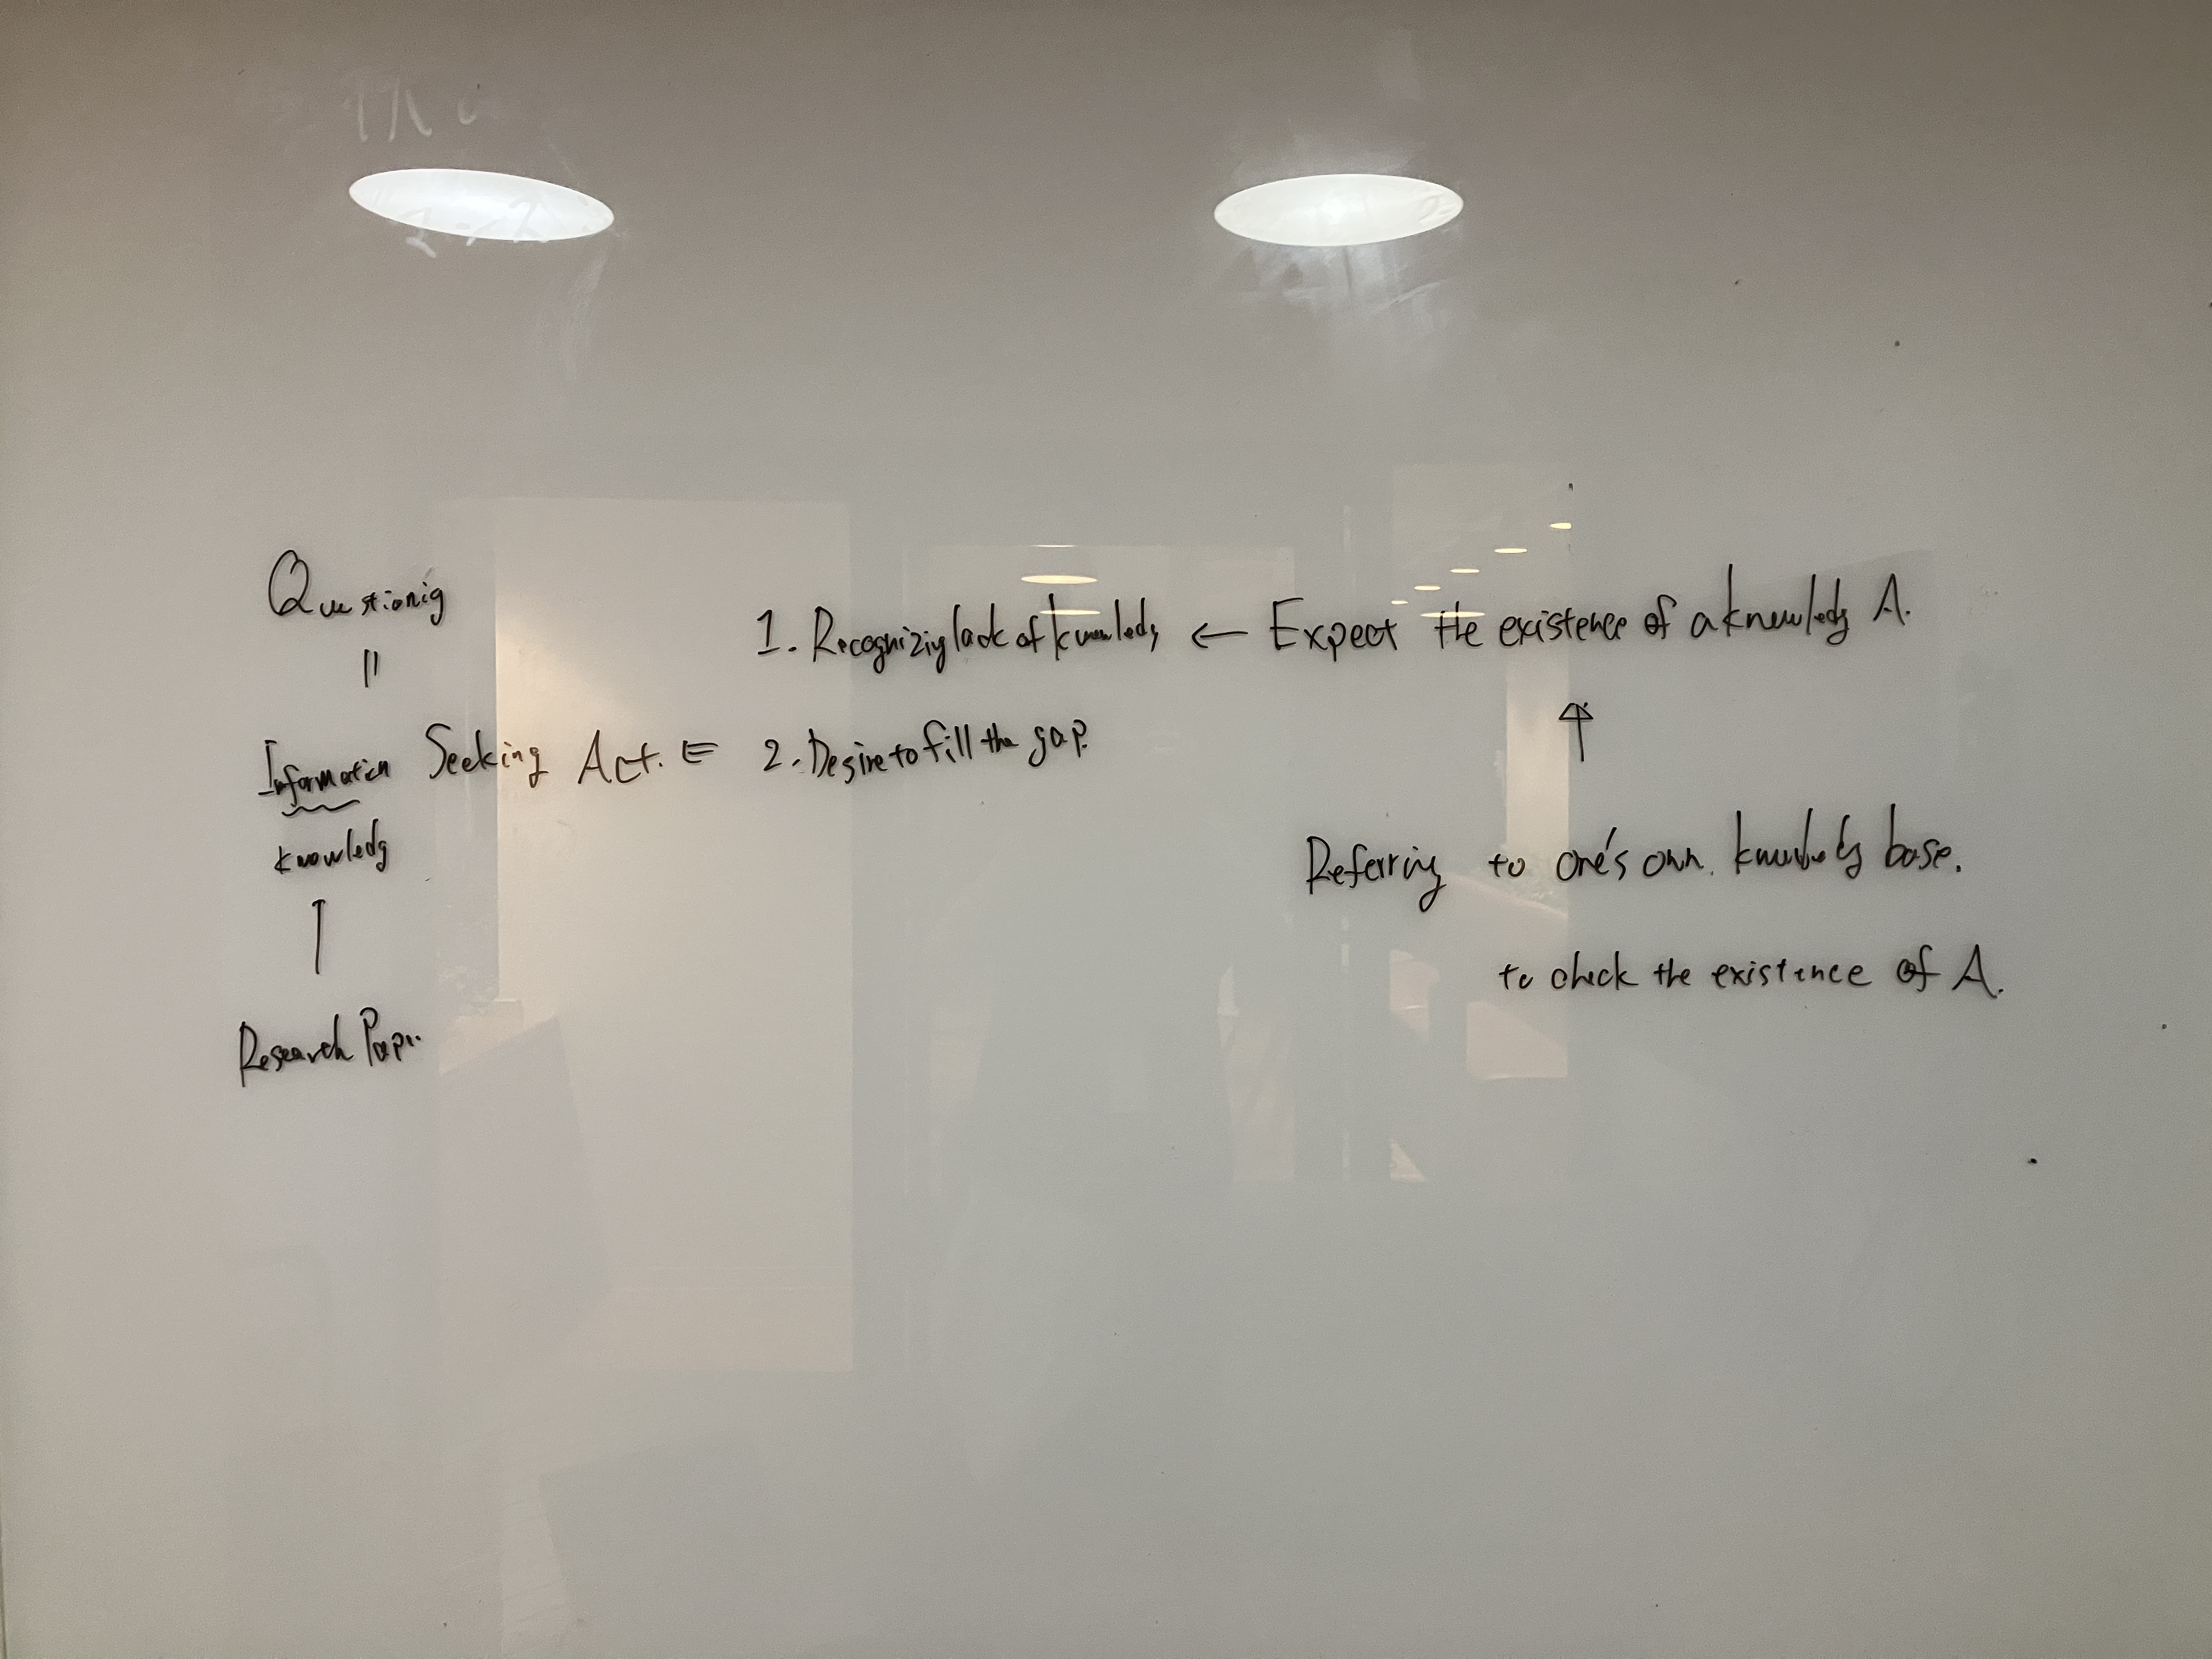
\includegraphics[width=\textwidth]{figs/question_formulation.jpg}
%     \caption{question construction}
%     \label{fig:enter-label}
% \end{figure}

% \subsubsection{How to Identify the Necessary Knowledge for Achieving a Goal?}
% In this situation, we need to consider how to identify the knowledge required to achieve our objectives. Typically, when given a goal, we start by listing the necessary elements to accomplish it. For example, to achieve general artificial intelligence, we may think that it requires the ability to handle language, understand the real world, be proficient in mathematics, and align with human values. To understand the real world, for instance, we may need the capability for interacting with the physical world, processing visual information, and so on. These requirements can be further broken down into multiple necessary elements. By repeating this process, we can narrow down the specific tasks that can be directly addressed. Then, the required knowledge to accomplish those tasks is demanded, and that's where it directly connects to the research question.

% Several things are happening here. Firstly, listing the elements necessary for achieving the goal means generating sub-goals from the main goal. However, it's always a challenging problem to evaluate how a particular sub-goal contributes to the achievement of a given goal. Especially in the case of research, the target might be an too general and ambitious vision that nobody has achieved before, so we need to think about what needs to be done to break it down into appropriate sub-problems. In other words, it is necessary to construct a tree with nodes representing sub-goals.

% Secondly, it is necessary to identify the most important sub-goal from the selected candidate sub-goals. Since only one question can be addressed in the end, it is necessary to select a single sub-goal using some evaluation criteria. This may not be a problem if the sub-goals can be judged on the same evaluation criteria, but in many cases, unrelated sub-goals may arise. For example, to create general artificial intelligence, the development of machine learning theory may be equally important as the advancement of semiconductor technology. However, it may be difficult to compare their importance on the same evaluation axis.

% Thirdly, the question to ultimately arrive at must be verifiable. If the question is not specific, meaningful verification cannot be performed. Overly broad or ambiguous questions can result in countless or trivial answers, or they may be too unclear to provide practical answers. Increasing the specificity of the question corresponds to deepening the depth of the sub-goal tree, so it may be important to construct a sufficiently deep tree and find an efficient way to navigate it. The verifiability is constrained by the knowledge, resources, such as funding and technology, that we currently have. Therefore, when conducting verification in reality, it is necessary to consider such feasibility. Whether to tackle a question with high feasibility or to further divide it into more subtasks for its realization is a matter of judgment. In any case, it is necessary to appropriately evaluate such feasibility. The scope of feasibility is vast, so it is a challenging problem to determine how to consider it in creating intelligent systems.

% Here, we discussed what needs to be done to construct questions that generate the necessary knowledge to achieve the goal. We believe that research that can generate knowledge that is expected to contribute to the achievement of the goal, and that has not been revealed in previous studies, can be considered as ``important'' research. In that sense, it may be important to consider how to achieve the automation of research in this direction.

% In this discussion, we have only touched upon a limited number of points that we personally consider important. However, we believe that there are other important points that should be considered. By seriously reflecting on ``how questions are currently being constructed,'' these points are expected to become clearer.

% Also, in this discussion, we considered the method of outputting questions from the goal through the construction and exploration of a tree structure. However, as mentioned by the predecessors, if an end-to-end approach ultimately becomes a powerful method, it may be more desirable to consider a direction in which questions are directly output from the goal. In particular, even when performing multi-step reasoning, it seems more natural to improve reasoning abilities using the recently developed approaches to multi-step logical reasoning, rather than explicitly considering tree structures. While the development of methods for multi-step reasoning is undoubtedly important in pursuing this direction, this is not a point that needs to be emphasized here as it is being addressed not only in the context of research automation but also more generally. As a discussion focused on the automation of research, it may be worth considering the construction of higher-quality datasets for goals and research questions. For example, it may be possible to construct a dataset by extracting only the ultimate goal and the research questions actually solved from the introductions of papers.

% However, an important point to note here is that the research questions created by humans so far are not necessarily optimal for achieving research goals. Firstly, machines may be capable of maximizing the objective better than humans due to cognitive constraints. Secondly, not all human research has been conducted by working backward from a clear goal. Some studies were conducted simply because they seemed interesting while reading papers. Additionally, as mentioned earlier, abstraction has significantly advanced science, but there are cases where the study of abstraction itself is the

%  objective rather than abstraction in some specific cases. In this regard, simply learning from human data without imitation may constrain the potential capabilities that machines can possess. Therefore, it becomes important to consider how to formulate the maximization of the probability of achieving research goals as a problem, rather than naive learning from human data.

% \subsubsection{How to Search Necessary Knowledge and Recognize the Lack of Knowledge?}
% There are various methods to determine whether the desired knowledge already exists. Typically, it is considered that candidates can be narrowed down in two steps. First, since research papers are composed of questions and their corresponding answers, one can search for papers that have similar questions and answers to the desired knowledge. Once these papers are found, the validity of their verification methods is evaluated. If it is determined that sufficient verification has not been conducted, it can be concluded that the knowledge does not exist.

% In this case, the knowledge itself was considered as the research paper database, so the process involved searching and individually assessing the papers as described above. However, for example, if the knowledge is represented by the distributed representation of a machine itself, the need for the search step may be eliminated. Nevertheless, even in this case, the reliability of the machine's judgment can only be trusted if it has appropriately assessed the effectiveness of its own verification. Therefore, the ability to understand and evaluate verification seems essential in determining the novelty of research.

% \textcolor{red}{TODO: Is question construction information retrieval??}

% \subsubsection{Multiple Reasons for Unknownness}
% new, unimportant, difficult, unnoticed, ... etc.

% \subsubsection{Finding ``Important'' but Unnoticed Questions}

% \subsubsection{Conclusion}
% In summary, the following abilities are required to generate research questions for achieving a specific goal:

% \begin{enumerate}
%     \item Predicting the necessary knowledge from the goal:
%     \begin{enumerate}
%         \item Solving prediction and reasoning problems with long-range relationships.
%         \item Refining knowledge by appropriately incorporating ``good'' qualities such as importance, concreteness, ethics, etc.
%     \end{enumerate}
%     \item Determing the existence of expected knowledge:
%     \begin{enumerate}
%         \item Searching for knowledge directly related to the expected knowledge.
%         \item Determining whether the knowledge has been properly validated.
%     \end{enumerate}
% \end{enumerate}

% 1.a is related to research on improving the reasoning capabilities of machine learning models and on generating intermediate goals in reinforcement learning. If these research fields produce significant results, they can be directly applied. In this sense, it might be beneficial to seek cooperation from those who are actively conducting research in these areas. One of the unique aspects of long-distance inference problems that we think is interesting is the fact that the goal is something that has never been achieved before. This means that you cannot naively learn from data and need to generalize outside of the distribution. Therefore, it's essential to acquire skills not just to recognize patterns but to properly trace the path of reasoning. Moreover, because the goal has not been realized, sub-goals and the paths that connect them are ultimately based on the accumulation of hypothesis generation. In this sense, it can be said that this is a highly uncertain inference. This implies that the choice of which node to select is far from self-evident compared to other logical inference problems. Furthermore, there is the issue of the complexity of the distance between the goal and the question, which is far more intricate than, for example, games or planning everyday trips. For instance, to truly achieve the goal, it may be necessary to build large-scale apparatus like particle accelerators from scratch. This also means that the temporal distance between the goal and the current location is very long. Therefore, it becomes a problem that feedback on how much solving the question contributed to the goal is significantly delayed. While I've only listed a few examples here, there may be other unique challenges and issues that become more serious in research. It will be necessary to work on refining these technical challenges into specific research tasks through discussions with researchers in reasoning and planning.

% 1.b is specific to the automation of research. We first need to be aware that these "good" aspects do not occur naturally. As mentioned before, these are non-epistemic values, so the more autonomy the agent has, the more these must be consciously incorporated. To create an intelligence that constructs ``good'' questions, we first need to understand what we consider a ``good'' question. Also, it's important to turn our attention to things that are not currently considered ``good,'' but should be deemed as ``good'' in essence. Only then can we discuss how to align that value with the agent. Therefore, we think we should start by listing the criteria for determining the ``goodness'' of a question. For this, discussions in the philosophy of science and meta-sciences like the Science of Science may be referenced. Alternatively, large-scale surveys of researchers engaged in actual research could also be important. Once the value is clarified, we might be able to think about creating an intelligence equipped with these values using the value alignment techniques that are currently being developed.

% 2.a is a discussion of Information Retrieval itself. As previously mentioned, research is a process of searching for information from various sources and utilizing it to produce knowledge. Therefore, information retrieval technology is essential, not just for constructing questions. So, it's crucial how much we can get information retrieval researchers involved in this. One of the things strongly related to the automation of research within information retrieval is the search for papers. We will discuss this in the section on information retrieval.

% 2.b is a unique discussion about the automation of research. However, this greatly overlaps with the content to be discussed in the chapter on hypothesis testing. Specifically, what's needed here is the evaluation of testing, whereas what's required for the automation of hypothesis testing is the generation of testing. In this sense, the latter discussion includes the discussion here. Therefore, we will refrain from discussing this here and touch on it later.

% we have listed what we believe are important elements in the construction of questions. However, these are considered important under the assumptions mentioned earlier. For instance, if the goal is not to acquire knowledge necessary for achieving an objective, but to generate knowledge that an individual finds interesting, the necessary elements in question construction (particularly in parts 1.a and 1.b) would change. As previously mentioned, the value of knowledge is determined in relation to context and there's a high degree of uncertainty about how the value of knowledge will evolve in the future. This makes it fundamentally important to have a diverse range of ways to generate questions. The object achievement is highly prevalent and is expected to produce ``important'' knowledge, which is why it is discussed here. However, it is important to discuss what other ways of formulating questions could exist and how they can be implemented.


% \subsection{Hypothesis Verification}
% verification of hypotheses allows for any action to be considered as long as it is subject to verification, meaning that it updates an individual's beliefs. In this sense, it is believed to be extremely difficult to fully automate the act of verification universally and unconditionally. To achieve complete automation, the realization of physical robots capable of movements at least equivalent to humans in the real world would be necessary, which goes beyond the scope of developing intelligence.

% Therefore, to automate this process, it is necessary to proceed with automation gradually, starting from what can be automated. Two directions can be considered as ways to mitigate this problem. The first direction is to break down the verification process and gradually automate parts that are relatively feasible for automation using machine learning. The second direction is to prioritize the automation of research domains where verification is relatively easy. 

% \subsubsection{Start from Verification Design}

% First, let's explain the former direction. As mentioned earlier, we believe that the verification process can be divided into three stages: formulating a verification plan, preparing for the execution of the verification plan, and executing the verification plan. Among these stages, the execution of the verification plan and the preparation for it require interaction with the physical world in many fields. For example, in certain fields, you may need to purchase and raise rats for training, while in others, you may need to observe physical objects directly. On the other hand, formulating a verification plan is a process that is purely confined to the human mind in a wide range of fields. Of course, in many cases, interacting directly with the physical world can lead to better verification plans, but it is important to note that it is not an absolute requirement. Therefore, to automate the execution and preparation of verification, it is suggested that the power of robotics researchers be leveraged, while machine learning researchers should focus on automating the formulation of verification plans. 

% \subsubsection{Narrowing Down the Domain}

% Next, let's discuss the second direction, which is to prioritize the automation of verification in research domains where it is relatively easy. As mentioned earlier, the greatest challenge for machine learning researchers in the unified automation of hypothesis verification is the fact that some fields require interaction with the physical world for the execution of verification preparation. Therefore, the second direction is to focus on narrowing down the domains where the execution and preparation of verification take place solely within the computer world and aim for complete automation in these domains.

% Many machine learning research and information-related research fall into this domain. However, it remains challenging, but the problem has shifted from reproducing arbitrary movements in physical space to realizing arbitrary operations on a computer, which can be seen as a relaxation of the problem. Research on tool usage using language models that has gained momentum in recent years and research on browser automation are directly related to the automation of this process. If arbitrary operations on a computer can be automated as an extension of these studies, it becomes more realistic for many information-related research fields, fields that can be reduced to pure symbolic operations, and fields where all the resources required for research exist on the web to be fully automated.

% From this explanation, it is also clear that in this part of the verification process, which requires execution and preparation, even understanding what verification is may not be necessary as long as the verification plan is perfectly created. The only point at issue is the realization of arbitrary actions within the target space. In other words, as mentioned earlier, these two directions can be pursued in parallel.

% Based on the above, we propose that the automation of fields requiring interaction with the physical world be left to capable robotics researchers, and machine learning researchers should initially aim for complete automation of research confined to the computer space. Regarding the autonomy of automating verification plans, it is advisable to first create intelligence that can understand the verification concepts that humans perform. 

% Although we can proceed them in parallel, we believe that we should prioritize the automation of verification plan development. This is because, as mentioned repeatedly, the execution and preparation of verification do not require verification-specific capabilities. It aims to acquire more general abilities, and many individuals who are not pursuing research automation are also working towards achieving this. However, the realization of verification plan capabilities is a point of particular interest for those pursuing research automation, and it has not received sufficient attention nor progress unless driven by individuals aiming for research automation. Therefore, we believe that prioritizing the automation in this area would be beneficial.


% The ultimate goal is to create an artificial intelligence capable of conducting research autonomously. Therefore, in addition to automating individual modules of research, it is necessary to create a system that can autonomously carry out the entire research process from start to finish. Building such a research process pipeline is one of the sub-goals we aim for.

% This is similar to the pipelines discussed in MLOps in the context of machine learning or scientific workflows mentioned in previous studies. However, unlike those, we envision a system that does not include processing that is heavily dependent on specific research domains or tasks. Instead, we formalize it as a pipeline consisting of modules for question construction, hypothesis generation, and planning and execution of verification, as discussed in Chapter 2. This system autonomously constructs and validates hypotheses for any given question with an unknown answer.


% \section{Others}



\chapter{Conclusion}


% \bibliographystyle{unsrt}
\bibliographystyle{apalike}
\bibliography{ref}

\appendix

\chapter{Additional Literature Review}

\chapter{Alignment}
Understanding is subjective, so there is a need to consider alignment. Even if the process of hypothesis generation is incomprehensible to humans, as long as the verification is connected to fundamental human beliefs, it can be said to be knowledge based on a common foundation with humans.

\chapter{Research Optimization}

\chapter{Research as Social Activity}
In this paper, we will discuss automation focused on the unique elements of knowledge production as mentioned above. However, research is a social endeavor. And that society has various levels, such as research labs, universities, and research ecosystems. Therefore, if we think about optimizing the whole activity of research, we need to think about optimizing these wholes. Although it is out of the scope of this paper and therefore not discussed this time, we would like to discuss this in the future.

\chapter{Research as Belief Update}

From the perspective that research is belief updating, the roles of question construction, hypothesis generation, and hypothesis verification can be represented in the following Fig. \ref{fig:beliefupdate}. 
\begin{figure}[htb]
    \centering
    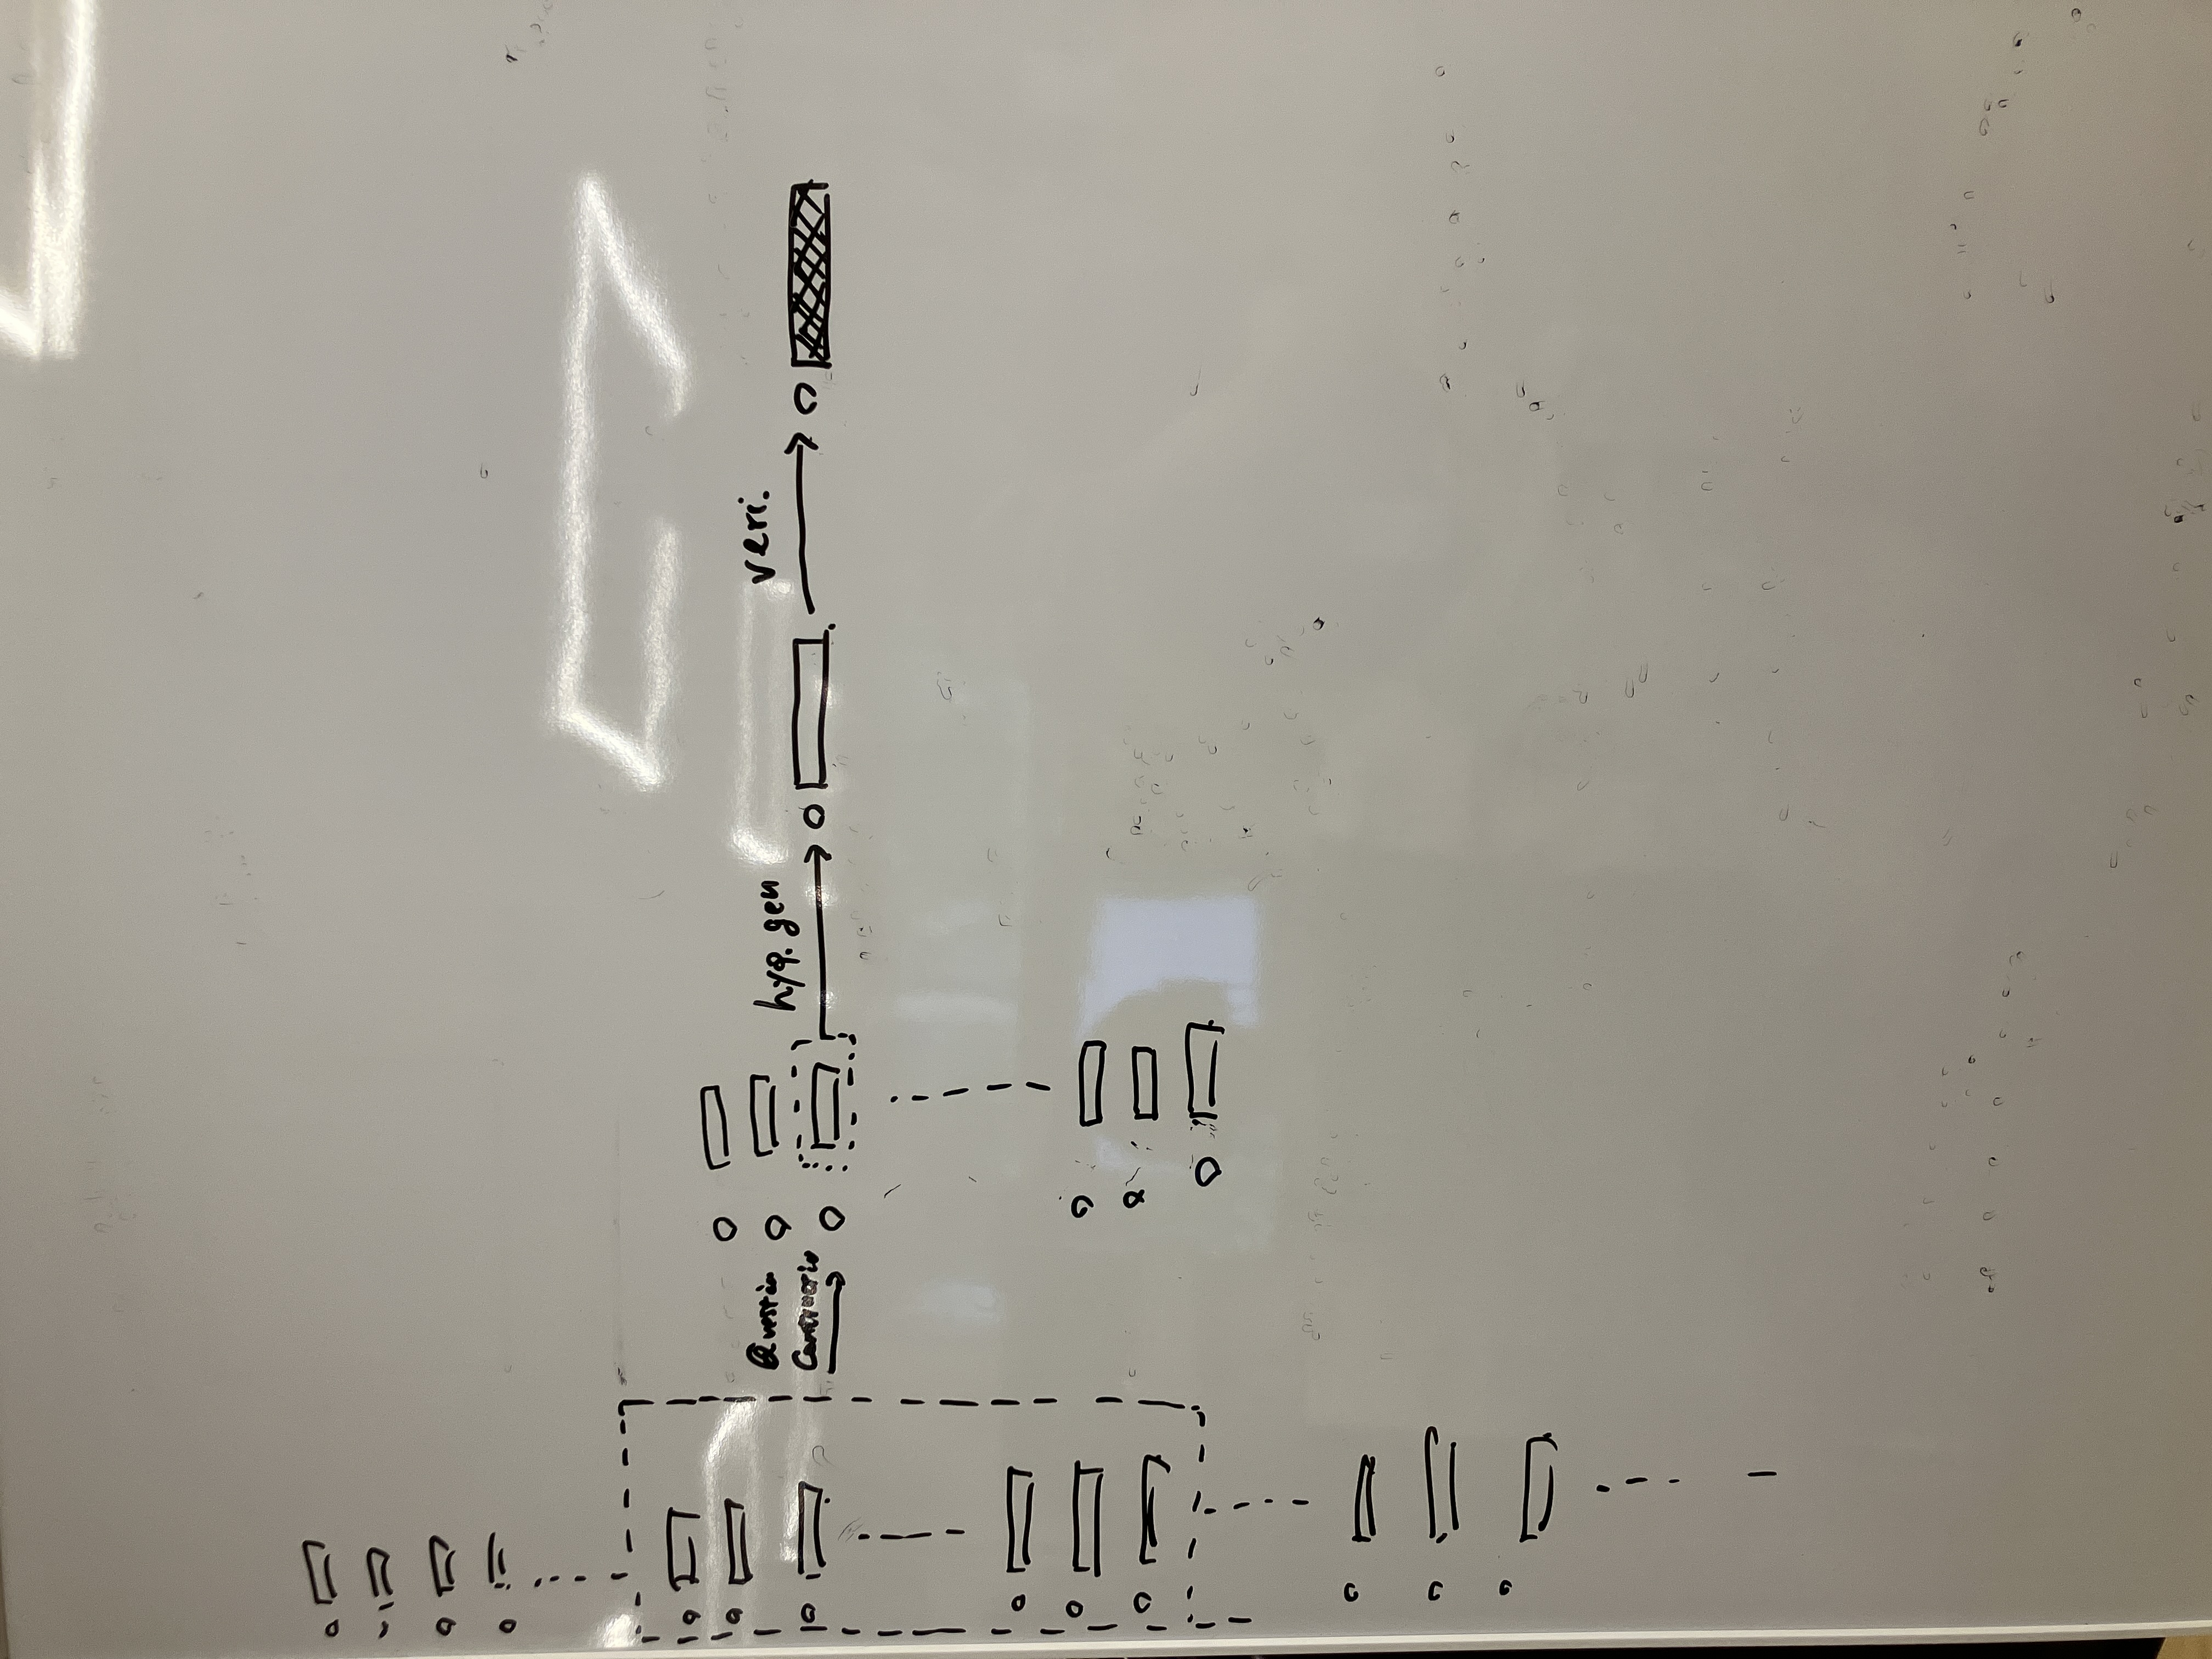
\includegraphics[width=\textwidth]{figs/beliefupdate.jpg}
    \caption{Research Process as Belief Update}
    \label{fig:beliefupdate}
\end{figure}
In the diagram, circles represent statements, and squares represent beliefs in response to those statements. Note that while circles were described as statements, they are not limited to textual representations as long as they are associated with beliefs. Beliefs are determined by the subject holding the belief (in this case, an agent) and the object of the belief (the statement), but please note that we are assuming a fixed agent in this context.

Firstly, in this world, there exist countless pairs of statements and corresponding beliefs (or latent beliefs). Posing a question corresponds to extracting a subset of unknown statements from this pool. More precisely, an unknown statement refers to a statement for which the agent is unsure whether to assign a strong or weak belief. Choosing corresponds to implicitly determining a function that assigns beliefs to each statement. For example, let's consider posing the question ``When did the universe begin?'' This answer to this question is unknown to humanity. By posing this question, the range of possible answers is narrowed down. However, it is not realistically possible for an agent to be aware of all statements and potential answers that could exist. Therefore, while we mentioned pairs of beliefs and statements, please consider that most of these beliefs are latent and potential.

Next, generating a hypothesis involves selecting one pair of a claim and a belief from among the potential claims that could serve as potential answers to the question. It is at this point, by choosing a hypothesis or considering multiple candidate hypotheses, that discourse becomes consciously acknowledged, and beliefs are substantively assigned. Finally, as we discussed in Chapter 2, verification involves gaining evidence for the belief in the chosen hypothesis, resulting in the updating of the belief state. The updated beliefs are represented in black in the diagram.


\end{document}